%% The Sigma_1 theory of non-structural subtyping is decidable.
%% LIPIcs format; build with `make` (latexmk -pdf main.tex). Sections live in sections/,
%% figures in figures/. Add the class option `anonymous' for a double-blind copy.
\documentclass[a4paper,USenglish,cleveref,thm-restate,numberwithinsect]{lipics-v2021}
%% Packages -----------------------------------------------------------------
\usepackage{mathtools}
\usepackage{booktabs}
\usepackage{longtable}
\usepackage{array}
\usepackage{enumitem}
\usepackage{xurl}
\usepackage{tikz}
\usetikzlibrary{automata,positioning,arrows.meta,decorations.pathreplacing,calc,fit,backgrounds,shapes.geometric,patterns}


%% Lean identifiers: typewriter, with URL-style line breaking.
%% Breaks are allowed only after a dot or an underscore (xurl would break anywhere).
\DeclareUrlCommand\lean{\urlstyle{tt}\def\UrlBreaks{\do\.\do\_}\def\UrlBigBreaks{}\def\UrlNoBreaks{}}

%% Long formulas: allow slightly looser lines instead of overfull boxes.
\setlength{\emergencystretch}{2em}

%% Signature, trees and the order --------------------------------------------
\newcommand{\Bot}{\bot}
\newcommand{\Top}{\top}
\newcommand{\BF}{\{\Bot,f\}}
\newcommand{\BFT}{\{\Bot,f,\Top\}}
\newcommand{\Dir}{[n]}                          % argument positions 1..n
\newcommand{\pol}{\operatorname{pol}}           % polarity of a path
\newcommand{\dom}{\operatorname{dom}}
\newcommand{\Trees}{\mathcal{T}}                % all trees
\newcommand{\TreesReg}{\mathcal{T}_{\mathrm{reg}}}
\newcommand{\TreesFin}{\mathcal{T}_{\mathrm{fin}}}
\newcommand{\Cls}{\mathcal{C}}                  % a class of trees
\newcommand{\fall}{f^{\omega}}                  % the tree with f at every path
\newcommand{\eps}{\varepsilon}
\newcommand{\entails}{\models}

%% Words ----------------------------------------------------------------------
\newcommand{\len}[1]{\lvert #1\rvert}
\newcommand{\wsub}[3]{#1[#2{:}#3]}             % factor w[i:j]
\newcommand{\wpre}[2]{#1[{:}#2]}               % prefix w[:i]
\newcommand{\wsuf}[2]{#1[#2{:}]}               % suffix w[i:]
\newcommand{\pre}{\preceq}                     % prefix order on words
\newcommand{\Alp}{A}                           % alphabet of a reader
\newcommand{\lcsuf}{\operatorname{lcs}}        % length of the longest common suffix (in blocks)

%% Cones, atoms and derivations -------------------------------------------
\newcommand{\Cone}[2]{C^{#1}(#2)}              % cone of sign #1 of the tree #2
\newcommand{\sgp}{{+}}
\newcommand{\sgm}{{-}}
\newcommand{\flip}[1]{\overline{#1}}           % opposite sign
\newcommand{\SV}{V^{\pm}}                      % signed variables
\newcommand{\Atoms}{\mathcal{A}}
\newcommand{\der}{\vdash}                      % derivation by rules
\newcommand{\mv}{\Rightarrow}                  % derivation by moves
\newcommand{\LC}{\mathrm{LC}}                  % least closure
\newcommand{\Hull}{\mathrm{Hull}}
\newcommand{\NegV}{\mathsf{Neg}}               % signed variables with a forbidden root
\newcommand{\FctV}{\mathsf{Fct}}               % signed variables reachable from facts
\newcommand{\Up}{\mathsf{U}}                   % upper run
\newcommand{\Dn}{\mathsf{D}}                   % lower run
\newcommand{\stepU}{\delta^{\uparrow}}
\newcommand{\stepD}{\delta^{\downarrow}}

%% Readers and holes ----------------------------------------------------------
\newcommand{\Rej}{\mathsf{Rej}}
\newcommand{\Adm}{\mathsf{Adm}}
\newcommand{\dead}{\dagger}
\newcommand{\Chan}{\mathsf{Ch}}                % channel
\newcommand{\Vis}{\mathsf{Vis}}                % visited states
\newcommand{\tot}[1]{\lVert #1\rVert}          % total length of a tuple
\newcommand{\dominates}{\sqsubseteq}
\newcommand{\Hole}{\mathsf{H}}                 % small-hole bound
\newcommand{\TailB}{\Lambda}                   % rejected-tail bound
\newcommand{\FreshB}{\mathsf{J}}               % fresh-tuple bound
\newcommand{\expo}{\operatorname{exp}}         % iterated exponential
\newcommand{\cov}{\widehat}                    % cover of a hole

%% Fresh tuples ---------------------------------------------------------------
\newcommand{\mk}[2]{\sigma^{#1}_{#2}}          % marker of level #1 of coordinate #2
\newcommand{\Act}{\mathrm{Act}}
\newcommand{\Anc}{\mathrm{Anc}}
\newcommand{\dcut}{\operatorname{cut}}
\newcommand{\lab}{\operatorname{lab}}
\newcommand{\Marg}{\mathsf{m}}                 % deletion margin

%% Rejected tails ---------------------------------------------------------------
\newcommand{\onset}{\operatorname{on}}
\newcommand{\per}{\operatorname{per}}
\newcommand{\Dict}{\mathcal{D}}
\newcommand{\node}{\operatorname{node}}
\newcommand{\gap}{\operatorname{gap}}
\newcommand{\Lb}{\mathsf{L}}                   % search length for closed factors
\newcommand{\Wb}{\mathsf{B}}                   % window envelope
\newcommand{\Fb}{\Phi}                         % factor length bound
\newcommand{\Qc}{\mathsf{Q}}                   % number of periodic factors: 4+2(k-1)(N-1)
\newcommand{\cmap}{\operatorname{im}}          % cut map (image of a retained cut) of a deletion of positions
\newcommand{\proj}{\operatorname{pr}}          % projection of the cover of a hole

%% Hyperlink targets of numbered statements -----------------------------------
%% The class numbers theorems within sections, but the hyperref anchors use only
%% the number inside the section (definition.1 in Sections 2 and 4, ...), so links
%% to later statements jumped to earlier ones. Include the section in the anchor.
\makeatletter
\@for\pf@env:={theorem,lemma,corollary,proposition,exercise,definition,conjecture,%
  observation,example,note,remark,claim}\do{%
  \@ifundefined{theH\pf@env}{}{%
    \expandafter\def\csname theH\pf@env\endcsname{\theHsection.\arabic{theorem}}}}
\makeatother

%% Lists of references without a serial comma, as in the rest of the text.
\renewcommand{\creflastconjunction}{ and\nobreakspace}

\hideLIPIcs
\nolinenumbers

\bibliographystyle{plainurl}

\title{The \texorpdfstring{$\Sigma_1$}{Sigma-1} Theory of Non-Structural Subtyping Is Decidable}
\titlerunning{The \texorpdfstring{$\Sigma_1$}{Sigma-1} Theory of Non-Structural Subtyping Is Decidable}

\author{Yaoyu Zhao}{EPFL, Switzerland}{yaoyu.zhao@epfl.ch}{}{}
\authorrunning{Y. Zhao}
\Copyright{Yaoyu Zhao}

\ccsdesc[500]{Theory of computation~Type theory}
\ccsdesc[500]{Theory of computation~Logic and verification}
\ccsdesc[300]{Theory of computation~Formal languages and automata theory}

\keywords{subtyping, subtype constraints, entailment, first-order theory, decidability,
combinatorics on words, automata, mechanized proof}

\supplement{The Lean development: \url{https://github.com/noti0na1/deci-sigma1}}

\begin{document}
\maketitle

\begin{abstract}
%% abstract -- body only; input inside the abstract environment of main.tex.
Subtype constraints are inequalities $s\le t$ between type expressions with
unknowns. With a least type $\Bot$ and a greatest type $\Top$, the subtype order
is non-structural: it relates trees of different shapes. For a binary
covariant constructor, the first-order theory of this order is undecidable, already for
sentences with the quantifier prefix $\exists\forall\exists$, whereas satisfiability of a conjunction of constraints
is decidable in polynomial time and entailment between constraints was shown
decidable only recently. We determine the $\Sigma_1$ level of the quantifier
hierarchy: it is decidable whether a Boolean combination of existential
($\Sigma_1$) and universal ($\Pi_1$) sentences over subtype constraints is true.
The result holds for the signature $\BFT$ with one constructor $f$ of any arity
and any variance, in particular for function types, over arbitrary, regular and
finite trees, and for the signature $\BF$ with a covariant constructor.
Satisfiability and entailment are special cases, and so is the entailment of a
disjunction of $k$ inequalities, to which every sentence reduces. A disjunction can
be entailed although none of its disjuncts is, so the $k$ failures of a
countermodel have to be realized by one solution.

We reduce a countermodel to a \emph{hole} of a finite automaton with $k$ start
states: a tuple of $k$ words, one witness path for each failed inequality, such
that no forbidden pair of states occurs where the rest of one word is a prefix
of the rest of another word. The central technical theorem bounds the total
length of a shortest hole. Its proof has two parts. Words that can be continued forever are
replaced by ultimately periodic continuations whose mutual constraints form a
system of difference constraints, and their periodic stretches are then compressed.
The remaining tuples are shortened by deleting repeated blocks of a hierarchy
of markers in all words at once. The bound is elementary: four iterated
exponentials of a number that is polynomial in the size of the automaton for
a fixed number of queries, and five iterated exponentials of a polynomial in
the size of the sentence, while the problem is PSPACE-hard. The decision procedures, their
correctness and the elementary bound are mechanized in Lean~4.

\end{abstract}

\section{Introduction}
\label{sec:intro}

Type inference with subtyping collects the typing requirements of a program as
\emph{subtype constraints} $s\le t$ between type expressions with unknowns
\cite{Mitchell91,FuhMishra90,AikenWimmers93,EifrigSmithTrifonov95,Pottier98}.
Types are finite or infinite trees. When the type language has a least type
$\Bot$ and a greatest type $\Top$, the subtype order is \emph{non-structural}:
$\Bot\le t\le\Top$ holds for every tree $t$, so the order relates trees of
different shapes. For instance, with a binary constructor $f$ that is covariant
in both arguments,
\[
  f(\Bot,\,f(\Bot,\Bot))\;\le\;f(f(\Top,\Bot),\,\Top),
\]
although the two trees have no common shape.

Three questions about a \emph{constraint} $\Gamma$, a finite set of such
inequalities read as their conjunction, have been studied for this order. \emph{Satisfiability} asks whether $\Gamma$ has a solution; it
is decidable in polynomial time
\cite{KozenPalsbergSchwartzbach94,PalsbergWandOKeefe97}. \emph{Entailment}
asks whether every solution of $\Gamma$ satisfies a further inequality
$x\le y$; it is the basis of constraint simplification
\cite{Pottier96,TrifonovSmith96,Rehof97,Pottier01}. Its decidability, posed
by Rehof in 1996 as Problem~16 of the TLCA list of open problems
\cite{Rehof96TLCA}, was studied by Niehren and Priesnitz with automata
\cite{NiehrenPriesnitz99,NiehrenPriesnitz03} and settled positively only
recently \cite{Zhao26}. Finally, the full \emph{first-order theory} of the
order is undecidable \cite{SuAikenNiehrenPriesnitzTreinen02}, and for a
binary covariant constructor, with or without $\Top$, this already holds for
sentences with the quantifier prefix $\exists\forall\exists$
\cite{Zhao26U}.

Satisfiability is an existential ($\Sigma_1$) sentence
$\exists\bar x.\,\bigwedge\Gamma$ in which no negation occurs, and entailment
is a universal ($\Pi_1$) sentence
$\forall\bar x.\,\neg\bigwedge\Gamma\vee x\le y$ of a special form: its
quantifier-free part has a single positive inequality. This paper decides the
whole first level of the quantifier hierarchy.

\begin{theorem}[Main theorem]\label{thm:main}
Let $f$ be a constructor of arity $n\ge0$, each of whose arguments is covariant
or contravariant. It is decidable whether a Boolean combination of $\Sigma_1$
and $\Pi_1$ sentences over subtype constraints with the signature $\BFT$ is
true, over arbitrary trees, over regular trees, and over finite trees. A
sentence is true over the regular trees exactly when it is true over all
trees. The same holds for the signature $\BF$ when $f$ is covariant. The
decision procedures are uniform in the arity and the variance.
\end{theorem}

The function type constructor is the case $n=2$ with a contravariant first
argument. Since a $\Pi_1$ sentence is the negation of a $\Sigma_1$ sentence,
the sentences of the theorem are the Boolean combinations of $\Sigma_1$
sentences; we call the set of the true ones the \emph{$\Sigma_1$ theory}.
Truth over finite trees can differ from truth over all trees: for a unary
constructor, $\exists x.\,x\le f(x)\wedge f(x)\le x$ is true over regular
trees, with the infinite tree $f(f(\cdots))$ as witness, and false over finite
trees.

\subparagraph*{Disjunctive entailment.}
A $\Sigma_1$ sentence is true exactly when some clause of a disjunctive normal
form of its quantifier-free part has a solution. After every compound subterm
is named by a variable, such a clause has the form
\begin{equation}\label{eq:intro-clause}
  \Gamma\;\wedge\;\neg(x_1\le y_1)\;\wedge\;\dots\;\wedge\;\neg(x_k\le y_k),
\end{equation}
where $\Gamma$ is a constraint, a conjunction of inequalities, and
$x_1,y_1,\dots,x_k,y_k$ are variables. It has a solution exactly when
$\Gamma$ does \emph{not} entail the disjunction
$x_1\le y_1\vee\dots\vee x_k\le y_k$. So the theorem is equivalent to the
decidability of \emph{disjunctive entailment}
\[
  \Gamma\;\entails\;x_1\le y_1\vee\dots\vee x_k\le y_k,
\]
uniformly in the number $k$ of \emph{queries}. Plain entailment is the case
$k=1$ and satisfiability the case $k=0$.

Disjunctive entailment does not reduce to plain entailment in any direct way,
because a disjunction can be entailed although none of its disjuncts is. For
the function type constructor every tree is $\Bot$ or lies above the least
function type $f(\Top,\Bot)$, so $\forall x.\;x\le\Bot\vee f(\Top,\Bot)\le
x$ is true, but neither disjunct holds for all $x$. A countermodel of a
disjunction must refute all disjuncts with a single solution
(\cref{sec:sent-nonreduction}).

\subparagraph*{From countermodels to holes.}
A failed inequality $x\le y$ has a \emph{witness}: a path at which the labels
of the values of $x$ and $y$ are in the wrong order. For $k$ queries we obtain
$k$ witness paths $w_1,\dots,w_k$, which are words over the argument positions
$\{1,\dots,n\}$. We show that a tuple of words is the tuple of witnesses of
some countermodel exactly when it is a \emph{hole} of a finite automaton
compiled from $\Gamma$ and the queries, a \emph{structural reader}
(\cref{sec:readers}). The reader has one start state for each query. It reads
$w_i$ from the $i$th start state, and the tuple is a hole if every run stays
alive and ends in a \emph{rejected} state, and no \emph{admitted} pair of
states occurs at a \emph{comparison}: a pair of cuts, one in a word $w_i$ and
one in a word $w_j$, such that the rest of $w_j$ after its cut is a prefix of
the rest of $w_i$ after its cut. The words $w_i$ and $w_j$ may be the same
word or different ones. The pairs of states at the comparisons between $w_i$
and $w_j$ form the \emph{channel} between the two words. A comparison is a
place where a subtree that one witness forces into the solution meets a
subtree that another witness must keep out of it. Here a state is rejected
when the reader has rejected every way in which the constraint could refute
the witness, so rejected states are the good ones.

Whether a reader has a hole is not a regular property of the tuple of words,
since comparisons relate unboundedly long suffixes at unboundedly distant
cuts. Decidability follows from a bound on the length of a shortest hole. We
write $\expo_0(x)=x$ and $\expo_{h+1}(x)=2^{\expo_h(x)}$ for iterated
exponentials.

\begin{theorem}[Small holes]\label{thm:intro-small}
There is a computable function $\Hole$ such that every structural reader with
$N$ states and $k$ start states that has a hole has a hole of total length at
most $\Hole(k,N)$, whatever the size of its alphabet, and
\[
  \Hole(k,N)\;\le\;\expo_4\bigl((k+N+20)^{2k+6}\bigr).
\]
\end{theorem}

For a fixed number $k$ of queries the bound is four iterated exponentials
of a polynomial in $N$. A reader compiled from a constraint with $v$
variables has at most $2^{4v}+1$ states, so the witnesses of a countermodel can be chosen of length
at most five iterated exponentials of a polynomial in the size of the
sentence, and the $\Sigma_1$ theory is decidable in elementary space
(\cref{sec:complexity}). The problem is PSPACE-hard, because plain entailment
is \cite{HengleinRehof98}. The procedures establish decidability and an
elementary upper bound; they are not practical algorithms.

\subparagraph*{Why several queries are harder than one.}
The decision procedure for plain entailment \cite{Zhao26} also reduces a
countermodel to a hole and bounds a shortest hole, for readers with one start
state. Its argument does not extend to several words, for three reasons, which
are summarized in \cref{tab:intro-compare}.

\emph{Several witnesses in one solution.} With $k$ queries a hole is a tuple
of words, and there are comparisons between different words. Each
query can fail in two ways, at a path where the smaller side is too large or
at a path where the larger side is too small, so there is one reader for each
of the $2^k$ vectors of \emph{modes}.

\emph{Rejected tails.} A run enters the rejected states at some cut and then
stays in them. With one word, no admitted pair can involve a cut of the
\emph{rejected tail}, the part of the word after that cut, so a hole can be
cut off shortly after it. With several words, a cut in the rejected tail of
one word can still be the host of an admitted comparison with another word.
If the run can be continued forever, the tail may have to be long in order to
avoid the other words, and its length must be bounded independently of their
lengths. This is the largest part of the proof (\cref{sec:tails}). We replace
such tails by ultimately periodic words, \emph{rays}; we show that rays can be
chosen so that the constraints between their lengths form a solvable system
of difference constraints; and we compress the periodic stretches of the
resulting hole without creating an admitted pair on any channel.

\emph{Shortening all words together.} Deleting a block from one word of a
tuple can create a comparison with another word. The shortening of
\cref{sec:fresh} therefore follows one hierarchy of \emph{markers} for the
whole tuple and deletes the same repeated blocks from all words at the same
time.

\begin{table}[t]
\caption{Plain entailment and disjunctive entailment.}
\label{tab:intro-compare}
\small\setlength{\tabcolsep}{4pt}
\begin{tabular}{@{}>{\raggedright\arraybackslash}p{0.21\linewidth}>{\raggedright\arraybackslash}p{0.33\linewidth}>{\raggedright\arraybackslash}p{0.40\linewidth}@{}}
\toprule
 & Plain entailment \cite{Zhao26} & Disjunctive entailment (this paper) \\
\midrule
witness of a countermodel & one path & one path per query, all realized by one solution \\
\addlinespace
readers & one per failure side, with one start state & one per mode vector, $2^k$ in all, with $k$ start states \\
\addlinespace
comparisons & within one word & within and between the words of a tuple \\
\addlinespace
after the first rejection & no admitted pair; short tails & tails can still be hosts; bounded by rays and compression \\
\addlinespace
shortening & hierarchy of one word & one marker hierarchy, the same blocks deleted in all words \\
\bottomrule
\end{tabular}
\end{table}

\subparagraph*{Contributions.}
\Cref{fig:overview} shows the structure of the proof.
\begin{itemize}
\item We prove that the $\Sigma_1$ theory of non-structural subtyping is
  decidable for one constructor of any arity and variance with $\Bot$ and
  $\Top$, over arbitrary, regular and finite trees, and for a covariant
  constructor with $\Bot$ only (\cref{thm:main}, proved in
  \cref{sec:decision}).
\item We give an exact reduction of the countermodels of a disjunctive
  entailment to the holes of structural readers with $k$ start states
  (\cref{thm:reduction}).
\item We prove the small-hole theorem for structural readers
  (\cref{thm:small-hole}) from two results of independent interest in
  combinatorics on words with automata: a bound on rejected tails
  (\cref{thm:tails}) and a bound on minimal tuples of fresh words
  (\cref{thm:fresh}).
\item We show that the bound is elementary (\cref{thm:elementary}), discuss
  the gap to the PSPACE lower bound, and give families of sentences whose
  shortest witnesses are long (\cref{sec:complexity}).
\item The decision procedures, their correctness, the small-hole theorem and
  its elementary bound are mechanized in Lean~4 with Mathlib
  (\cref{sec:mechanization}).
\end{itemize}

%% overview -- the proof chain.
\begin{figure}[t]
\centering
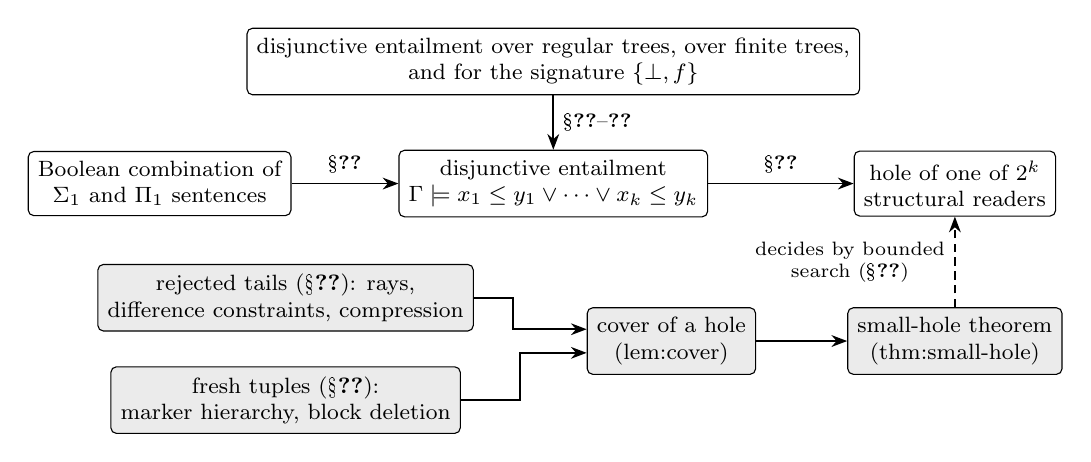
\begin{tikzpicture}[
  font=\footnotesize,
  box/.style={draw, rounded corners=2pt, align=center, inner sep=3.5pt, minimum height=8mm},
  thm/.style={box, fill=black!8},
  arr/.style={-{Stealth[length=2mm]}, semithick},
  lbl/.style={font=\scriptsize, align=center}]
%% first row: the reductions
\node[box] (sent) at (0,0) {Boolean combination of\\ $\Sigma_1$ and $\Pi_1$ sentences};
\node[box] (disj) at (5.0,0) {disjunctive entailment\\ $\Gamma\entails x_1\le y_1\vee\dots\vee x_k\le y_k$};
\node[box] (hole) at (10.1,0) {hole of one of $2^k$\\ structural readers};
\draw[arr] (sent) -- node[lbl, above] {\S\ref{sec:sentences}} (disj);
\draw[arr] (disj) -- node[lbl, above] {\S\ref{sec:readers}} (hole);
%% second row: the small-hole theorem and its two halves
\node[thm] (small) at (10.1,-2.0) {small-hole theorem\\ (\cref{thm:small-hole})};
\draw[arr, densely dashed] (small) -- node[lbl, left] {decides by bounded\\ search (\S\ref{sec:decision-arbitrary})} (hole);
\node[thm] (cover) at (6.5,-2.0) {cover of a hole\\ (\cref{lem:cover})};
\draw[arr] (cover) -- (small);
\node[thm] (tail) at (1.6,-1.45) {rejected tails (\S\ref{sec:tails}): rays,\\ difference constraints, compression};
\node[thm] (fresh) at (1.6,-2.75) {fresh tuples (\S\ref{sec:fresh}):\\ marker hierarchy, block deletion};
\draw[arr] (tail.east) -- ++(0.5,0) |- ([yshift=1.5mm]cover.west);
\draw[arr] (fresh.east) -- ++(0.75,0) |- ([yshift=-1.5mm]cover.west);
%% third row: classes of trees
\node[box] (cls) at (5.0,1.55) {disjunctive entailment over regular trees, over finite trees,\\
  and for the signature $\BF$};
\draw[arr] (cls) -- node[lbl, right] {\S\ref{sec:decision-regular}--\ref{sec:decision-bf}} (disj);
\end{tikzpicture}
\caption{The proof chain. Solid arrows between white boxes are reductions:
a sentence is reduced to disjunctive entailments (naming of subterms), and a
failed entailment over arbitrary trees with the signature $\BFT$ to a hole
of a finite reader (witnesses and modes); the other classes of trees and the
signature $\BF$ are reduced to this case. The gray boxes are the small-hole
theorem and the results it follows from. It bounds the length of a shortest
hole, so a bounded search decides the entailment (dashed arrow). Its proof
bounds the rejected tails of a hole and then the hole itself, read as a
tuple of fresh words in a larger automaton, its cover.}
\label{fig:overview}
\end{figure}


\Cref{sec:prelim} fixes trees, the order and sentences. \Cref{sec:sentences}
reduces sentences to disjunctive entailment, and \cref{sec:readers} reduces
disjunctive entailment to holes. \Cref{sec:overview} states the two bounds
and composes them. \Cref{sec:fresh,sec:tails} explain their proofs, with the
longer arguments in the appendices. \Cref{sec:decision} gives the decision
procedures, including regular and finite trees and the signature $\BF$, and
\cref{sec:complexity} the complexity bounds. \Cref{sec:mechanization}
describes the mechanization, \cref{sec:related} discusses related work, and
\cref{sec:future,sec:conclusion} discuss future work and conclude. The
notation is collected in \cref{app:notation}.

\section{Preliminaries}
\label{sec:prelim}

\subsection{Words}\label{sec:prelim-words}

Words are finite sequences of letters over a finite alphabet; $\eps$ is the
empty word and $\len{w}$ the length of $w$. A \emph{cut} of $w$ is a number
$a$ with $0\le a\le\len w$; it separates the prefix $\wpre wa$ of length $a$
from the suffix $\wsuf wa$, the \emph{rest} of $w$ after $a$. For cuts
$a\le b$, $\wsub wab$ is the factor between them, and the \emph{positions} of
$w$ are $0,\dots,\len w-1$, with the letter $w[p]$ at position $p$. We write
$u\pre v$ if $u$ is a prefix of $v$. Two words are \emph{comparable} if one is
a prefix of the other. A word $u$ \emph{ends at the cut} $e$ of $w$ if $u$ is
a suffix of $\wpre we$, and \emph{occurs at} $a$ if $u\pre\wsuf wa$. For
example, the cut $2$ of $w=0110$ separates $\wpre w2=01$ from the rest
$\wsuf w2=10$; the word $1$ occurs at the cuts $1$ and $2$ and ends at the
cuts $2$ and $3$; and the rest $10$ is comparable with $1$ and with $100$,
but not with $11$.

\subsection{Trees and the Subtype Order}\label{sec:prelim-trees}

We fix a constructor $f$ of arity $n\ge0$ and write $\Dir=\{1,\dots,n\}$ for
its argument positions. A \emph{path} is a word over $\Dir$.

\begin{definition}[Trees]\label{def:trees}
A \emph{tree} over $\BFT$ is a partial function $t$ from paths to
$\{\Bot,f,\Top\}$ whose domain $\dom t$ contains $\eps$ and is closed under
prefixes, such that for every $\pi\in\dom t$: if $t(\pi)=f$ then $\pi
i\in\dom t$ for every $i\in\Dir$, and otherwise $\pi i\notin\dom t$ for every
$i$. The elements of $\dom t$ are the \emph{positions} of $t$, and the
positions labeled $\Bot$ or $\Top$ are its \emph{leaves}. The \emph{subtree}
of $t$ at a position $\pi$ is the tree $\sigma\mapsto t(\pi\sigma)$.
\end{definition}

We write $\Bot$ and $\Top$ for the trees with the single position $\eps$,
and $f(t_1,\dots,t_n)$ for the tree with label $f$ at $\eps$ and subtree
$t_i$ at the position $i$. Trees may be infinite; for $n\ge1$ the tree
$\fall$ with $f$ at every path is an example. A tree is \emph{finite} if it
has finitely many positions and \emph{regular} if it has finitely many
distinct subtrees. We write $\Trees$, $\TreesReg$ and $\TreesFin$ for the
classes of all, regular and finite trees; $\TreesFin\subseteq\TreesReg
\subseteq\Trees$.

Each argument position is \emph{covariant} or \emph{contravariant}; the
\emph{variance} is a map $c\colon\Dir\to\{0,1\}$ with $c(i)=1$ for the
contravariant positions. The \emph{polarity} of a path
$\pi=i_1\cdots i_m$ is $\pol(\pi)=c(i_1)+\dots+c(i_m)\bmod 2$, the parity of
the number of contravariant steps. The labels are ordered $\Bot<f<\Top$.

\begin{definition}[Subtype order]\label{def:order}
For trees $s$ and $t$, $s\le t$ holds if for every path
$\pi\in\dom s\cap\dom t$,
\[
  s(\pi)\le t(\pi)\ \text{ if }\pol(\pi)=0,\qquad
  t(\pi)\le s(\pi)\ \text{ if }\pol(\pi)=1.
\]
\end{definition}

The order depends on the variance, which we keep fixed and do not write. It
is a partial order on trees (antisymmetry follows from \cref{thm:cones}),
and it is characterized on constructor trees by
the usual rules:
\begin{equation}\label{eq:order-rules}
\begin{aligned}
 &\Bot\le t\le\Top\quad\text{for every tree }t,\\
 &f(s_1,\dots,s_n)\le f(t_1,\dots,t_n)\iff
  \begin{cases}
    s_i\le t_i&\text{for every covariant }i,\\
    t_i\le s_i&\text{for every contravariant }i.
  \end{cases}
\end{aligned}
\end{equation}
Indeed $\Bot$ and $\Top$ have the single position $\eps$, of polarity $0$,
and the common paths of two constructor trees are $\eps$ and the paths
$i\pi$ with $\pi$ a common path of $s_i$ and $t_i$, where
$\pol(i\pi)=c(i)+\pol(\pi)$. The order is called \emph{non-structural}
because trees with different domains can be comparable; in the
\emph{structural} order, comparable trees have the same domain.

\begin{example}[Function types]\label{ex:arrows}
For function types, $n=2$, $f(a,b)$ is written $a\to b$, and $c(1)=1$,
$c(2)=0$. By \eqref{eq:order-rules}, $\Top\to\Bot\le a\to b\le\Bot\to\Top$
for all trees $a$ and $b$: the least function type accepts every argument
and returns the least type. So every tree other than $\Bot$ lies above
$\Top\to\Bot$. The types $\Bot\to\Bot$ and $\Top\to\Top$ are incomparable:
at the path $1$, of polarity $1$, the labels $\Bot$ and $\Top$ would have to
be in decreasing order for $\Bot\to\Bot\le\Top\to\Top$, and at the path $2$,
of polarity $0$, the labels $\Top$ and $\Bot$ would have to be in increasing
order for $\Top\to\Top\le\Bot\to\Bot$.
\end{example}

\subsection{Sentences}\label{sec:prelim-sentences}

Terms and quantifier-free formulas are built from variables $x,y,\dots$:
\[
  s,t ::= x\mid\Bot\mid\Top\mid f(t_1,\dots,t_n)
  \qquad\qquad
  \varphi,\psi ::= s\le t\mid\neg\varphi\mid\varphi\wedge\psi\mid\varphi\vee\psi,
\]
and $s=t$ abbreviates $s\le t\wedge t\le s$. Given an assignment $\rho$ of
trees to the variables, a term denotes a tree and a formula is true or false,
with $\le$ interpreted by the subtype order. A \emph{$\Sigma_1$ sentence} is
$\exists x_1\dots x_m.\,\varphi$ and a \emph{$\Pi_1$ sentence} is $\forall
x_1\dots x_m.\,\varphi$, where $\varphi$ is a quantifier-free formula with
variables among $x_1,\dots,x_m$.

A sentence is evaluated over a class $\Cls$ of trees: the quantifiers range
over the trees of $\Cls$. We consider the three classes $\Trees$, $\TreesReg$
and $\TreesFin$. Each of them contains $\Bot$ and $\Top$ and is closed under
the constructor, so every term denotes a tree of the class when its variables
do. A \emph{Boolean combination} of $\Sigma_1$ and $\Pi_1$ sentences is built
from such sentences with $\neg$, $\wedge$ and $\vee$; its truth over $\Cls$ is
defined from the truth of its component sentences.

\subsection{Constraints and Disjunctive Entailment}\label{sec:prelim-constraints}

The proof works with constraints in a flat form.

\begin{definition}[Flat constraints]\label{def:flat}
Let $V$ be a finite set of variables. A \emph{flat literal} over $V$ is one of
\[
  x\le y,\qquad f(x_1,\dots,x_n)\le y,\qquad y\le f(x_1,\dots,x_n),\qquad
  x=\Bot,\qquad x=\Top,
\]
with $x,y,x_1,\dots,x_n\in V$. A \emph{constraint} $\Gamma$ is a finite set
of flat literals, read as their conjunction. A \emph{solution} of $\Gamma$ in
a class $\Cls$ is an assignment $\rho\colon V\to\Cls$ that satisfies every
literal of $\Gamma$, and $\Gamma$ is \emph{satisfiable in $\Cls$} if it has a
solution in $\Cls$.
\end{definition}

\begin{definition}[Disjunctive entailment]\label{def:disj}
Let $\Gamma$ be a constraint over $V$, and let $(x_1,y_1)$, \dots, $(x_k,y_k)$ be
pairs of variables of $V$, the \emph{queries}; $k=0$ is allowed and queries
may repeat. Then $\Gamma$ \emph{entails} $x_1\le y_1\vee\dots\vee x_k\le
y_k$ over $\Cls$, written
\[
  \Gamma\entails_{\Cls}x_1\le y_1\vee\dots\vee x_k\le y_k,
\]
if every solution $\rho$ of $\Gamma$ in $\Cls$ satisfies $\rho(x_i)\le
\rho(y_i)$ for some $i$. A \emph{countermodel} in $\Cls$ is a solution of
$\Gamma$ in $\Cls$ with $\rho(x_i)\not\le\rho(y_i)$ for every $i$.
\end{definition}

The entailment holds exactly when there is no countermodel. For $k=0$ the
disjunction is empty, and the entailment holds exactly when $\Gamma$ is
unsatisfiable in $\Cls$. For $k=1$ this is \emph{plain} entailment
$\Gamma\entails_{\Cls}x\le y$, non-structural subtype entailment. With
$\bar x$ the variables of $\Gamma$, the classical problems are sentences of
our fragment:
\begin{center}
\small
\begin{tabular}{@{}ll@{}}
\toprule
Problem & Sentence \\
\midrule
$\Gamma$ is satisfiable & $\exists\bar x.\ \bigwedge\Gamma$ \\
$\Gamma$ entails $x\le y$ & $\forall\bar x.\ \neg\bigwedge\Gamma\vee x\le y$ \\
$\Gamma$ entails $x_1\le y_1\vee\dots\vee x_k\le y_k$ &
  $\forall\bar x.\ \neg\bigwedge\Gamma\vee x_1\le y_1\vee\dots\vee x_k\le y_k$ \\
\bottomrule
\end{tabular}
\end{center}
Here a literal $x=\Bot$ is the inequality $x\le\Bot$, and $x=\Top$ is
$\Top\le x$. \emph{Existential entailment} $\Gamma\entails\exists\bar z.\,
\Gamma'$, with further variables in the consequence, is a $\Pi_2$ sentence
and lies outside the $\Sigma_1$ theory; it is decided in \cite{Zhao26E}.

\begin{example}[A disjunction that no disjunct explains]\label{ex:unary}
Let $n=1$. Every tree is $f^m(\Bot)$, $f^m(\Top)$ or $\fall$, and any two
trees are comparable, whatever the variance. So the empty constraint entails
$x\le y\vee y\le x$ over each class, but it entails neither $x\le y$ nor
$y\le x$. For a binary covariant constructor the disjunction is not entailed:
$x=f(f(\Bot,\Bot),\Bot)$ and $y=f(\Bot,f(\Bot,\Bot))$ are incomparable. We
return to this example in \cref{ex:reader-unary}.
\end{example}

\subparagraph*{The signature $\BF$.}
A tree over $\BF$ is a tree in which $\Top$ does not occur. For this
signature we assume $f$ covariant, so the order is the inclusion of the sets
of positions labeled $f$. Terms have no $\Top$, flat constraints have no
literal $x=\Top$, and the variables range over the trees without $\Top$ of
the class. \Cref{sec:decision-bf} reduces this signature to $\BFT$.

\section{From Sentences to Disjunctive Entailment}
\label{sec:sentences}

This section reduces the truth of a sentence to finitely many disjunctive
entailments between flat constraints. The reduction is the same for every
class of trees that contains $\Bot$ and $\Top$ and is closed under the
constructor; we fix such a class $\Cls$.

\subsection{Normal Forms}\label{sec:sent-nf}

The truth value of a Boolean combination is computed from the truth values of
its component sentences, and a $\Pi_1$ sentence $\forall\bar x.\,\varphi$ is
true exactly when the $\Sigma_1$ sentence $\exists\bar x.\,\neg\varphi$ is
false. It therefore suffices to decide $\Sigma_1$ sentences.

A \emph{clause} is a conjunction of inequalities $s\le t$ and negated
inequalities $\neg(s\le t)$ between terms. Pushing negations inward and
distributing conjunctions over disjunctions turns a quantifier-free formula
$\varphi$ into an equivalent disjunction of clauses, a disjunctive normal form
of $\varphi$. Hence $\exists\bar x.\,\varphi$ is true over $\Cls$ exactly
when some clause of the normal form is \emph{realizable} in $\Cls$: some
assignment of trees of $\Cls$ to $\bar x$ makes all its conjuncts true.

\subsection{Naming Subterms}\label{sec:sent-flat}

Let $K$ be a clause. We introduce a variable $v_t$ for every term $t$ that
occurs in $K$, as a side of an inequality or as a subterm of one, with
$v_x=x$ for a variable $x$. The \emph{flat constraint} $\Gamma_K$ consists of
\begin{itemize}
\item $v_t=\Bot$ for $t=\Bot$, and $v_t=\Top$ for $t=\Top$, if these terms
  occur;
\item $f(v_{t_1},\dots,v_{t_n})\le v_t$ and $v_t\le f(v_{t_1},\dots,v_{t_n})$
  for every occurring term $t=f(t_1,\dots,t_n)$;
\item $v_s\le v_t$ for every inequality $s\le t$ of $K$.
\end{itemize}
The \emph{queries} of $K$ are the pairs $(v_s,v_t)$ for the negated
inequalities $\neg(s\le t)$ of $K$.

\begin{lemma}[Clauses]\label{lem:clause}
A clause $K$ with queries $(x_1,y_1),\dots,(x_k,y_k)$ is realizable in $\Cls$
if and only if $\Gamma_K\not\entails_{\Cls}x_1\le y_1\vee\dots\vee x_k\le
y_k$.
\end{lemma}

\begin{proof}
Let $\rho$ be an assignment in $\Cls$ of the variables of $K$ that realizes
$K$. Extend it by giving $v_t$ the value of the term $t$ under $\rho$; this
value lies in $\Cls$ because $\Cls$ contains $\Bot$ and $\Top$ and is closed
under the constructor. The first two groups of literals of $\Gamma_K$ hold
because the order is reflexive, the third because $\rho$ satisfies the
inequalities of $K$, and every query fails because $\rho$ satisfies the
negated inequalities. So the extension is a countermodel. Conversely, let
$\rho$ be a countermodel in $\Cls$. Since the order is antisymmetric, the two
literals for $t=f(t_1,\dots,t_n)$ give
$\rho(v_t)=f(\rho(v_{t_1}),\dots,\rho(v_{t_n}))$, so by induction on terms
$\rho(v_t)$ is the value of $t$ under the restriction of $\rho$ to the
variables of $K$. This restriction then satisfies every inequality of $K$,
by the third group, and no inequality $s\le t$ that is negated in $K$,
because $\rho$ refutes the query $(v_s,v_t)$.
\end{proof}

\begin{example}\label{ex:clause}
The sentence $\forall x.\;x\le\Bot\vee f(\Top,\Bot)\le x$ is the negation of
$\exists x.\;\neg(x\le\Bot)\wedge\neg(f(\Top,\Bot)\le x)$, whose body is a
single clause. Its flat constraint over the variables $x,b,t,a$ is
\[
  \Gamma=\{\,b=\Bot,\quad t=\Top,\quad f(t,b)\le a,\quad a\le f(t,b)\,\},
\]
with the queries $(x,b)$ and $(a,x)$. By \cref{lem:clause} the sentence is
true over $\Cls$ if and only if $\Gamma\entails_{\Cls}x\le b\vee a\le x$.
\end{example}

\begin{proposition}[Reduction to disjunctive entailment]\label{prop:sentences}
Suppose disjunctive entailment between flat constraints over $\Cls$ is
decidable, uniformly in the number of queries. Then it is decidable whether a
Boolean combination of $\Sigma_1$ and $\Pi_1$ sentences is true over $\Cls$.
Moreover, if two classes give every disjunctive entailment the same truth
value, they give every such sentence the same truth value.
\end{proposition}

\begin{proof}
By \cref{sec:sent-nf} it suffices to treat a $\Sigma_1$ sentence, which is
true exactly when one of the finitely many clauses of a normal form of its
body is realizable. By \cref{lem:clause} this is the failure of a disjunctive
entailment that is computed from the clause. The second statement follows
because the reduction does not depend on the class.
\end{proof}

The number of queries is the number of negated inequalities of a clause, so
the reduction needs disjunctive entailment for every $k$, and a single
decision procedure that takes $k$ as part of its input.

\subsection{Disjunctive Entailment Does Not Reduce to Plain Entailment}
\label{sec:sent-nonreduction}

Consider function types (\cref{ex:arrows}) and the entailment of
\cref{ex:clause},
\begin{equation}\label{eq:arrow-disj}
  \Gamma\;\entails\;x\le b\;\vee\;a\le x
  \qquad\text{with }b=\Bot\text{ and }a=\Top\to\Bot\text{ in every solution.}
\end{equation}
It holds, since every tree is $\Bot$ or lies above the least function type.
But $\Gamma$ entails neither $x\le b$, refuted by $x=\Top\to\Bot$, nor $a\le
x$, refuted by $x=\Bot$. For a covariant constructor, $f(\Bot,\dots,\Bot)$
plays the role of $\Top\to\Bot$. So deciding the disjuncts one at a time is
not enough, and countermodels of the single disjuncts do not help: a
countermodel of the disjunction must refute every disjunct with one
solution, and the two refuting values of $x$ above do not combine into one.
Moving negated disjuncts into the constraint takes us outside plain
entailment as well: $\Gamma\entails\varphi_1\vee\varphi_2$ holds if and only
if $\Gamma\wedge\neg\varphi_1\entails\varphi_2$, but $\neg\varphi_1$ is not
a constraint, and plain entailment allows only constraints on the left.
The $k$ failures therefore have to be decided jointly. The next section
describes what it means for $k$ failures to be realized by one solution.

\section{Witnesses, Modes and Readers}
\label{sec:readers}

This section characterizes the countermodels of a disjunctive entailment over
arbitrary trees by the holes of finite automata. We first represent trees by
two sets of paths, in which the order becomes inclusion and a constraint
becomes a set of implications between atoms
(\cref{sec:readers-cones,sec:readers-atoms}). A failed query then has a
witness path, in one of two modes (\cref{sec:readers-modes}), and a family of
witnesses belongs to one solution exactly under three conditions on
derivations (\cref{sec:readers-realization}). Finite automata follow these
derivations along the witness paths (\cref{sec:readers-runs}), which gives
the readers and the reduction
(\cref{sec:readers-def,sec:readers-reduction}). The representation by leaf
cones is that of \cite{Zhao26E}; proofs omitted here are in
\cref{app:reduction}. Throughout, trees are trees over $\BFT$ and
assignments range over all trees.

\subsection{Leaf Cones}\label{sec:readers-cones}

\begin{definition}[Signs and cones]\label{def:cones}
The \emph{sign} of a leaf $v$ of a tree $t$ is $\sgp$ if $t(v)=\Top$ and
$\pol(v)=0$, or $t(v)=\Bot$ and $\pol(v)=1$; otherwise it is $\sgm$. For a
sign $s\in\{\sgp,\sgm\}$, the \emph{cone} of sign $s$ of $t$ is
\[
  \Cone st=\{\,w\in\Dir^*\mid\text{some prefix of $w$ is a leaf of $t$ of sign $s$}\,\}.
\]
We write $\flip s$ for the opposite sign.
\end{definition}

For a covariant constructor all polarities are $0$, so $\Cone{\sgp}t$ is the
set of paths along which $t$ reaches $\Top$ and $\Cone{\sgm}t$ the set of
paths along which it reaches $\Bot$; \cref{fig:tree-witness} shows an
example. With contravariant arguments the two labels exchange their roles at
paths of polarity $1$. A path has at most one prefix that is a leaf, and it
has none exactly when it is a position labeled $f$. A set $L$ of paths is
\emph{extension closed} if $w\in L$ implies $wi\in L$ for every $i\in\Dir$.

\begin{theorem}[Leaf representation]\label{thm:cones}
\begin{enumerate}
\item\label{it:cones-pair} For every tree $t$, the cones $\Cone{\sgp}t$ and
  $\Cone{\sgm}t$ are disjoint and extension closed. Conversely, every pair of
  disjoint extension-closed sets of paths is the pair of cones of exactly one
  tree.
\item\label{it:cones-order} For all trees $t$ and $u$:\quad
  $t\le u\iff\Cone{\sgp}t\subseteq\Cone{\sgp}u$ and
  $\Cone{\sgm}u\subseteq\Cone{\sgm}t$.
\item\label{it:cones-node} $\eps\in\Cone{\sgp}t$ iff $t=\Top$, and
  $\eps\in\Cone{\sgm}t$ iff $t=\Bot$. If $t=f(t_1,\dots,t_n)$, then for every
  $i\in\Dir$, path $w$ and sign $s$: $iw\in\Cone st$ iff
  $w\in\Cone{s}{t_i}$ when $i$ is covariant, and iff
  $w\in\Cone{\flip s}{t_i}$ when $i$ is contravariant.
\end{enumerate}
\end{theorem}

So going up in the order adds leaves of sign $\sgp$ and removes leaves of
sign $\sgm$. The variance enters only through the signs of the leaves; there
are two cones for each tree, whatever the arity.

%% tree-witness -- two trees and the witness path of a failed inequality.
\begin{figure}[t]
\centering
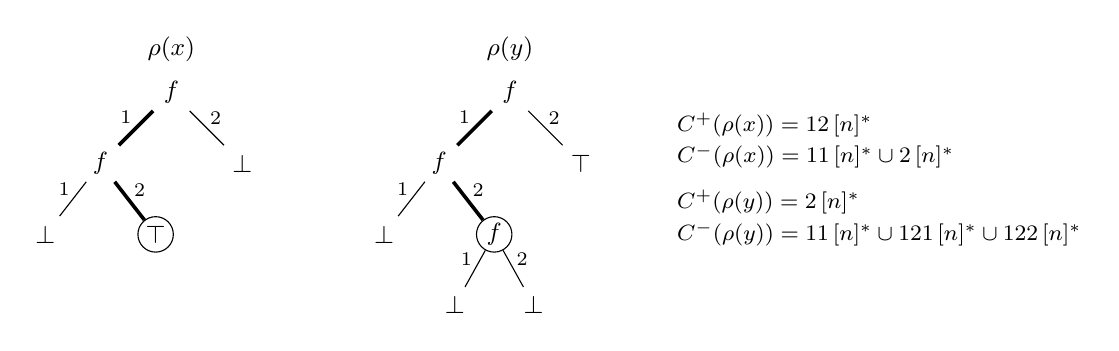
\begin{tikzpicture}[
  font=\small,
  nd/.style={inner sep=1.5pt, minimum size=4.5mm},
  mkd/.style={nd, draw, circle, inner sep=0.5pt},
  ed/.style={thin},
  wit/.style={line width=1.3pt},
  lb/.style={font=\scriptsize, inner sep=1pt}]
%% the tree of x
\begin{scope}
  \node[nd] (r) at (0,0) {$f$};
  \node[nd] (a) at (-0.9,-0.9) {$f$};
  \node[nd] (b) at (0.9,-0.9) {$\Bot$};
  \node[nd] (aa) at (-1.6,-1.8) {$\Bot$};
  \node[mkd] (ab) at (-0.2,-1.8) {$\Top$};
  \draw[wit] (r) -- node[lb, above left] {$1$} (a);
  \draw[ed] (r) -- node[lb, above right] {$2$} (b);
  \draw[ed] (a) -- node[lb, above left] {$1$} (aa);
  \draw[wit] (a) -- node[lb, above right] {$2$} (ab);
  \node at (0,0.55) {$\rho(x)$};
\end{scope}
%% the tree of y
\begin{scope}[xshift=4.3cm]
  \node[nd] (r) at (0,0) {$f$};
  \node[nd] (a) at (-0.9,-0.9) {$f$};
  \node[nd] (b) at (0.9,-0.9) {$\Top$};
  \node[nd] (aa) at (-1.6,-1.8) {$\Bot$};
  \node[mkd] (ab) at (-0.2,-1.8) {$f$};
  \node[nd] (aba) at (-0.7,-2.7) {$\Bot$};
  \node[nd] (abb) at (0.3,-2.7) {$\Bot$};
  \draw[wit] (r) -- node[lb, above left] {$1$} (a);
  \draw[ed] (r) -- node[lb, above right] {$2$} (b);
  \draw[ed] (a) -- node[lb, above left] {$1$} (aa);
  \draw[wit] (a) -- node[lb, above right] {$2$} (ab);
  \draw[ed] (ab) -- node[lb, above left] {$1$} (aba);
  \draw[ed] (ab) -- node[lb, above right] {$2$} (abb);
  \node at (0,0.55) {$\rho(y)$};
\end{scope}
\node[align=left, font=\footnotesize, anchor=west] at (6.3,-1.1)
  {$\Cone{\sgp}{\rho(x)}=12\,\Dir^*$\\[2pt]
   $\Cone{\sgm}{\rho(x)}=11\,\Dir^*\cup 2\,\Dir^*$\\[7pt]
   $\Cone{\sgp}{\rho(y)}=2\,\Dir^*$\\[2pt]
   $\Cone{\sgm}{\rho(y)}=11\,\Dir^*\cup121\,\Dir^*\cup122\,\Dir^*$};
\end{tikzpicture}
\caption{A witness of $\rho(x)\not\le\rho(y)$ for a binary covariant
constructor. Along the path $w=12$ (thick) the tree $\rho(x)$ reaches $\Top$
and $\rho(y)$ does not: $w\in\Cone{\sgp}{\rho(x)}\setminus\Cone{\sgp}{\rho(y)}$.
In the terms of \cref{sec:readers-modes} the query $(x,y)$ fails in mode
$\Top$ at $w$, with the seed $(x^{\sgp},w)$ and the exclusion
$(y^{\sgp},w)$.}
\label{fig:tree-witness}
\end{figure}


\subsection{Solutions as Closed Sets of Atoms}\label{sec:readers-atoms}

Let $\Gamma$ be a constraint over $V$. A \emph{signed variable} is a pair
$x^s$ of a variable and a sign; $\SV$ is the set of signed variables and
$\flip{x^s}=x^{\flip s}$. An \emph{atom} is a pair $(p,w)$ of a signed
variable and a path, and $\flip{(p,w)}=(\flip p,w)$ is its \emph{opposite}.
An assignment $\rho$ determines the set of atoms
\[
  S_\rho=\{\,(x^s,w)\mid w\in\Cone s{\rho(x)}\,\}.
\]
For an argument position $i$ we write $x^{[i]}$ for $x^{\sgp}$ if $i$ is
covariant and for $x^{\sgm}$ if $i$ is contravariant. \Cref{tab:clauses}
associates with every literal of $\Gamma$ a set of \emph{moves}, implications
between two atoms, together with \emph{facts}, atoms that must hold, and
\emph{forbidden atoms}, which must not. The \emph{rules} of $\Gamma$ are
its moves and the \emph{extensions} $(p,w)\to(p,wi)$, for all atoms $(p,w)$
and all $i\in\Dir$.

\begin{table}[t]
\caption{The rule form of the flat literals, for all paths $w$ and all
$i\in\Dir$.}
\label{tab:clauses}
\centering\small
\begin{tabular}{@{}llll@{}}
\toprule
Literal & Moves & Facts & Forbidden atoms \\
\midrule
$x\le y$ & $(x^{\sgp},w)\to(y^{\sgp},w)$,\quad $(y^{\sgm},w)\to(x^{\sgm},w)$ & & \\[2pt]
$f(x_1,\dots,x_n)\le y$ & $(x_i^{[i]},w)\to(y^{\sgp},iw)$,\quad
   $(y^{\sgm},iw)\to(\flip{x_i^{[i]}},w)$ & & $(y^{\sgm},\eps)$ \\[2pt]
$y\le f(x_1,\dots,x_n)$ & $(y^{\sgp},iw)\to(x_i^{[i]},w)$,\quad
   $(\flip{x_i^{[i]}},w)\to(y^{\sgm},iw)$ & & $(y^{\sgp},\eps)$ \\[2pt]
$x=\Bot$ & & $(x^{\sgm},\eps)$ & \\
$x=\Top$ & & $(x^{\sgp},\eps)$ & \\
\bottomrule
\end{tabular}
\end{table}

A set $S$ of atoms is \emph{closed} if it is closed under the rules,
\emph{consistent} if it contains no atom together with its opposite, and a
\emph{solution set} of $\Gamma$ if it is closed and consistent, contains the
facts and contains no forbidden atom.

\begin{lemma}[Rule form]\label{lem:clause-form}
The map $\rho\mapsto S_\rho$ is a bijection from the solutions of $\Gamma$
onto the solution sets of $\Gamma$.
\end{lemma}

The proof translates each literal with \cref{thm:cones}: for instance,
$f(x_1,\dots,x_n)\le y$ says that the cone of sign $\sgp$ of the constructor
tree, which consists of the paths $iw$ with $w$ in a cone of $\rho(x_i)$, is
contained in that of $\rho(y)$, and that the cone of sign $\sgm$ of
$\rho(y)$ is contained in that of the constructor tree, which does not
contain $\eps$.

We write $a\der b$ if the atom $b$ is \emph{derivable} from the atom $a$ by
finitely many rules, and $a\mv b$ if it is derivable by moves only. The
\emph{least closure} $\LC$ of $\Gamma$ is the set of atoms derivable from
facts. It is closed and contained in every solution set, so $\Gamma$ is
satisfiable if and only if $\LC$ is consistent and contains no forbidden
atom, and then $\LC$ is the least solution set.

The moves read the path of an atom as a stack whose top is its first letter:
a move replaces the signed variable and pops or pushes one letter at the top,
or leaves the path unchanged. Extensions add letters at the bottom. Two
properties of the moves are used throughout.

\begin{lemma}[Duality and normal form]\label{lem:duality}
\begin{enumerate}
\item\label{it:dual} If $a\to b$ is a move, so is $\flip b\to\flip a$. Hence
  $a\mv b$ implies $\flip b\mv\flip a$.
\item\label{it:ext-first} $(p,u)\der(q,v)$ if and only if
  $(p,u\sigma)\mv(q,v)$ for some path $\sigma$.
\end{enumerate}
\end{lemma}

Two finite sets of signed variables record where the forbidden atoms and the
facts enter. Both kinds of atoms have the empty path, and we let
\begin{equation}\label{eq:neg-fct}
\begin{aligned}
  \NegV&=\{\,r\in\SV\mid(r,\eps)\text{ is a forbidden atom of }\Gamma\,\},\\
  \FctV&=\{\,r\in\SV\mid(p,\eps)\mv(r,\eps)\text{ for some fact }(p,\eps)
  \text{ of }\Gamma\,\}.
\end{aligned}
\end{equation}
An atom whose derivations reach a signed variable of $\NegV$ with the empty
path cannot belong to a solution set, and an atom that is reached from a
signed variable of $\FctV$ with the empty path belongs to every solution
set.

\begin{example}[Rules of a small constraint]\label{ex:guard-rules}
Let $f$ be binary and covariant, and let
\[
  \Gamma=\{\,u\le f(u,u),\quad x\le u,\quad y=\Bot\,\}
\]
over the variables $x,y,u$. The inequality $u\le f(u,u)$ ensures that
$\Top$ does not occur in $u$ (this is the guard of
\cref{sec:decision-bf}); since $x\le u$, $\Top$ does not occur in $x$
either, and $y$ is $\Bot$. By \cref{tab:clauses} the moves are, for all paths $w$ and
$i\in\{1,2\}$,
\begin{align*}
  (u^{\sgp},iw)&\to(u^{\sgp},w), & (u^{\sgm},w)&\to(u^{\sgm},iw)
    &&\text{from }u\le f(u,u),\\
  (x^{\sgp},w)&\to(u^{\sgp},w), & (u^{\sgm},w)&\to(x^{\sgm},w)
    &&\text{from }x\le u.
\end{align*}
The first pops a letter, the second pushes one, and the last two keep the
path; in each row the second move is the dual of the first. The only forbidden atom is $(u^{\sgp},\eps)$ and the only fact is
$(y^{\sgm},\eps)$, so $\NegV=\{u^{\sgp}\}$ and $\FctV=\{y^{\sgm}\}$. The
least closure consists of the atoms $(y^{\sgm},w)$, which are derived from
the fact by extensions: it describes the solution with the least set of
atoms, $y=\Bot$ and $x=u=\fall$. The derivation
\[
  (x^{\sgp},12)\to(u^{\sgp},12)\to(u^{\sgp},2)\to(u^{\sgp},\eps)
\]
pops the path $12$ and ends in a forbidden atom. So no solution set contains
$(x^{\sgp},12)$: the tree of $x$ cannot reach $\Top$ along the path $12$,
nor along any other path, because every path can be popped in this way.
\end{example}

\subsection{Witnesses and Modes}\label{sec:readers-modes}

By \cref{thm:cones}\eqref{it:cones-order}, an inequality fails in one of two
ways.

\begin{lemma}[Witnesses]\label{lem:witness}
Let $\rho$ be an assignment and $(x,y)$ a query. Then $\rho(x)\not\le\rho(y)$
if and only if there are a path $w$ and a \emph{mode} $\mu\in\{\Top,\Bot\}$
such that
\begin{itemize}
\item $\mu=\Top$,\quad $(x^{\sgp},w)\in S_\rho$ and $(y^{\sgp},w)\notin
  S_\rho$;\quad or
\item $\mu=\Bot$,\quad $(y^{\sgm},w)\in S_\rho$ and $(x^{\sgm},w)\notin
  S_\rho$.
\end{itemize}
\end{lemma}

In mode $\Top$ the smaller side is too large along $w$: it has a leaf of
sign $\sgp$ that the larger side lacks. In mode $\Bot$ the larger side is too
small. We call the atom that must belong to $S_\rho$ the \emph{seed} of the
witness and the atom that must not belong to it the \emph{exclusion}; both
have the path $w$. For queries $(x_1,y_1),\dots,(x_k,y_k)$, a vector of modes
$\bar\mu=(\mu_1,\dots,\mu_k)$ and a tuple of paths $W=(w_1,\dots,w_k)$, we
write $A_i=(p_i,w_i)$ for the seed and $B_i=(p'_i,w_i)$ for the exclusion
of query $i$, so that
\begin{equation}\label{eq:seeds}
  (p_i,p'_i)=(x_i^{\sgp},y_i^{\sgp})\ \text{ if }\mu_i=\Top,\qquad
  (p_i,p'_i)=(y_i^{\sgm},x_i^{\sgm})\ \text{ if }\mu_i=\Bot.
\end{equation}
A solution $\rho$ of $\Gamma$ is a countermodel if and only if, for some
$\bar\mu$ and $W$, the set $S_\rho$ contains every $A_i$ and no $B_i$. The
signed variables $p_i,p'_i$ depend only on the queries and the modes; the
tuple $W$ is what the decision procedure has to find. In
\cref{fig:tree-witness}, for instance, the query $(x,y)$ fails in mode
$\Top$ with the witness $12$.

\subsection{Realization}\label{sec:readers-realization}

\begin{theorem}[Realization]\label{thm:realization}
Let $\Gamma$ be satisfiable over $\Trees$, and let $A_1,\dots,A_k$ and
$B_1,\dots,B_k$ be atoms. Some solution set of $\Gamma$ contains every $A_i$
and no $B_i$ if and only if
\begin{enumerate}[label=\textup{(R\arabic*)}]
\item\label{it:R1} no $A_i$ derives a forbidden atom;
\item\label{it:R2} $B_i\notin\LC$ and $\flip{A_i}\notin\LC$, for every $i$;
\item\label{it:R3} $A_j\not\der B_i$ and $A_j\not\der\flip{A_i}$, for all
  $i$ and $j$, including $i=j$.
\end{enumerate}
In this case the \emph{hull} $\LC\cup\{b\mid A_j\der b\text{ for some }j\}$
is the least such solution set.
\end{theorem}

The conditions are clearly necessary: a solution set is closed, so it
contains the hull, and it is consistent and contains no forbidden atom. For
the converse one has to show that the hull is consistent. If it contained an
atom $b$ derived from $A_j$ together with $\flip b$ derived from $A_i$, the
duality of \cref{lem:duality} would turn the second derivation around and
compose it with the first into a derivation from $A_j$ toward
$\flip{A_i}$. The extensions, which have no dual, are handled by
\ref{it:R1}.

Condition \ref{it:R3} is where the $k$ witnesses interact. It involves pairs
of queries, and also a single query with itself: a seed must not derive its
own exclusion or its own opposite.

\subsection{Runs along a Path}\label{sec:readers-runs}

The conditions of \cref{thm:realization} are conditions on derivations
between atoms whose paths are the unknown words $w_i$. Two families of
finite sets summarize the derivations by moves along a path.

\begin{definition}[Upper and lower runs]\label{def:runs}
For a signed variable $p$ and a path $w$,
\[
  \Up(p,w)=\{\,r\in\SV\mid(p,w)\mv(r,\eps)\,\},\qquad
  \Dn(p,w)=\{\,r\in\SV\mid(r,\eps)\mv(p,w)\,\}.
\]
\end{definition}

The \emph{upper run} $\Up(p,w)$ collects the signed variables reached from
$(p,w)$ when the whole path has been popped, and the \emph{lower run}
$\Dn(p,w)$ those from which $(p,w)$ is built by pushing the whole path. Since
moves only see the top of the stack, $r\in\Up(p,w)$ also means that
$(p,w\sigma)\mv(r,\sigma)$ for every $\sigma$ by moves that never pop a
letter of $\sigma$, and similarly for $\Dn$. By duality,
$\Dn(p,w)=\{\flip r\mid r\in\Up(\flip p,w)\}$.

\begin{lemma}[Runs are deterministic]\label{lem:runs-det}
There are computable functions $\stepU,\stepD\colon 2^{\SV}\times\Dir\to
2^{\SV}$ such that $\Up(p,wi)=\stepU(\Up(p,w),i)$ and
$\Dn(p,wi)=\stepD(\Dn(p,w),i)$ for all $p$, $w$ and $i$. Moreover
$\stepU(P,i)=\varnothing$ whenever $P\cap\NegV=\varnothing$.
\end{lemma}

So both runs are computed by reading $w$ from the root, with two
deterministic automata whose states are sets of signed variables. The last
statement holds because a letter can be popped only from an atom
$(y^{\sgp},iw)$ with a literal $y\le f(\dots)$, or from $(y^{\sgm},iw)$ with a
literal $f(\dots)\le y$, and in both cases the signed variable lies in
$\NegV$.

\begin{lemma}[Derivations through cuts]\label{lem:cuts}
Let $(p,u)$ and $(q,v)$ be atoms with $\Up(p,u)\cap\NegV=\varnothing$. Then
$(p,u)\der(q,v)$ if and only if there are cuts $a$ of $u$ and $b$ of $v$
such that
\[
  \wsuf ua\pre\wsuf vb\qquad\text{and}\qquad
  \Up(p,\wpre ua)\cap\Dn(q,\wpre vb)\ne\varnothing.
\]
Moreover, $(p,u)$ derives a forbidden atom if and only if
$\Up(p,u)\cap\NegV\ne\varnothing$.
\end{lemma}

A derivation from $(p,u)$ first extends $u$, then pops a prefix of the path
down to a lowest point and pushes a prefix of $v$. The hypothesis says that
the pops do not go beyond $u$, so the lowest point is a cut $a$ of $u$, and
the rest $\wsuf ua$ is never touched: it survives as a prefix of the rest of
$v$. This is the origin of the comparisons ``the rest of one word is a prefix
of the rest of another word'' in the definition of holes. In
\cref{ex:guard-rules}, the atom $(u^{\sgm},2)$ derives $(x^{\sgm},12)$ by
pushing the letter $1$ and moving to $x^{\sgm}$. The cuts of the lemma are
$0$ in the path $2$ and $1$ in the path $12$: the rest $2$ is not touched,
and $\Up(u^{\sgm},\eps)=\{u^{\sgm},x^{\sgm}\}$ meets
$\Dn(x^{\sgm},1)=\{u^{\sgm}\}$. The same analysis,
applied to derivations from facts, shows that $(q,v)\in\LC$ if and only if
$\Dn(q,\wpre vb)$ meets the set $\FctV$ of \eqref{eq:neg-fct} for some cut
$b$ of $v$; this uses that $\Gamma$ is satisfiable.

\subsection{Structural Readers and Holes}\label{sec:readers-def}

We now define the automata and their holes abstractly. The alphabet is an
arbitrary finite set $\Alp$; in the reduction it is $\Dir$.

\begin{definition}[Structural reader]\label{def:reader}
A \emph{structural reader} with $k$ \emph{starts} over $\Alp$ consists of a
finite set $S$ of states, a transition function $\delta\colon S\times\Alp\to
S$, $k$ start states $s_1,\dots,s_k\in S$, which need not be distinct, a
\emph{dead}
state $\dead\in S$ with $\delta(\dead,c)=\dead$ for every letter $c$, a set
$\Rej\subseteq S\setminus\{\dead\}$ of \emph{rejected} states and a relation
$\Adm\subseteq S\times S$ of \emph{admitted} pairs, such that for every
$q\in\Rej$ and every letter $c$ with $\delta(q,c)\ne\dead$:
\begin{enumerate}[label=\textup{(S\arabic*)}]
\item\label{it:S1} $\delta(q,c)\in\Rej$;
\item\label{it:S2} $(q',\delta(q,c))\notin\Adm$ for every state $q'$.
\end{enumerate}
Its \emph{size} is $N=\len S$.
\end{definition}

The names anticipate the reduction of \cref{sec:readers-reduction}, where a
reader follows the derivations from the seed of a witness. A run is
\emph{dead} when the constraint alone already contradicts the witness. A
state is \emph{rejected} when the seed can no longer derive a forbidden
atom: the reader has rejected every way of refuting the witness by a
forbidden atom. So a rejected state is what a witness has to reach, although
the word may suggest the opposite. Condition \ref{it:S1} says that rejection
is permanent, and \ref{it:S2} that a state reached after a rejected state is
never the second component of an admitted pair. A pair of states is
\emph{admitted} when it shows a derivation from the seed of one witness
that contradicts a witness, the same one or another; such pairs matter only
at the places defined next.

Let $W=(w_1,\dots,w_k)$ be a tuple of words. The word $w_i$ is read from
$s_i$; we write $q_i(a)=\delta^*(s_i,\wpre{w_i}a)$ for the state of
coordinate $i$ at the cut $a$, and $q_i(\len{w_i})$ is its \emph{endpoint}.
The \emph{total length} of $W$ is $\tot W=\len{w_1}+\dots+\len{w_k}$.

\begin{definition}[Comparisons, channels and holes]\label{def:hole}
Let $i$ and $j$ be coordinates, possibly equal. A \emph{comparison} from the
\emph{host} $i$ to the \emph{target} $j$ is a pair $(a,b)$ of a cut $a$ of
$w_i$ and a cut $b$ of $w_j$ such that $\wsuf{w_j}b\pre\wsuf{w_i}a$: the
rest of the target is a prefix of the rest of the host. The pair of states
$(q_i(a),q_j(b))$ is the \emph{channel pair} at this comparison, and the
\emph{channel} from $i$ to $j$ is the set of all channel pairs,
\[
  \Chan_{ij}(W)=\{\,(q_i(a),q_j(b))\mid a\text{ a cut of }w_i,\ b\text{ a cut
  of }w_j,\ \wsuf{w_j}b\pre\wsuf{w_i}a\,\}.
\]
Coordinate $i$ is \emph{eligible} if $q_i(a)\ne\dead$ for every cut $a$ and
its endpoint is rejected. The tuple $W$ is a \emph{hole} if every coordinate
is eligible and $\Chan_{ij}(W)\cap\Adm=\varnothing$ for all $i$ and $j$.
\end{definition}

All cuts are included, also the two ends: at $b=\len{w_j}$ the rest of the
target is empty, so $(a,b)$ is a comparison for every cut $a$ of the host.
For example, in the tuple $(0110,\,10)$ the comparisons from the host $1$ to
the target $2$ are $(2,0)$, since $10$ is the rest of $0110$ after the cut
$2$, then $(0,1)$ and $(3,1)$, since the rest $0$ of the target is a prefix
of the rests $0110$ and $0$, and $(a,2)$ for the five cuts $a$ of the host.
In a pair $(q,q')\in\Adm$ the first component is the state of a host and the
second the state of a target; the relation need not be symmetric.
\Cref{fig:reader-hole}(a) shows a comparison and its channel pair.

For an eligible coordinate, \ref{it:S1} gives a \emph{first rejected cut}
$J_i$: the states $q_i(a)$ are rejected exactly for $a\ge J_i$. The prefix
$\wpre{w_i}{J_i}$ is the \emph{head} of $w_i$ and the suffix
$\wsuf{w_i}{J_i}$ its \emph{rejected tail}. By \ref{it:S2}, the target cut of
an admitted channel pair is at most $J_j$. So the tail of a word is never
involved as a target, but it can be involved as a host, and for $i=j$ a
channel pair has $a\le b$.

%% reader-hole -- a channel between two words of a tuple, and the reader of the worked example.
\begin{figure}[t]
\centering
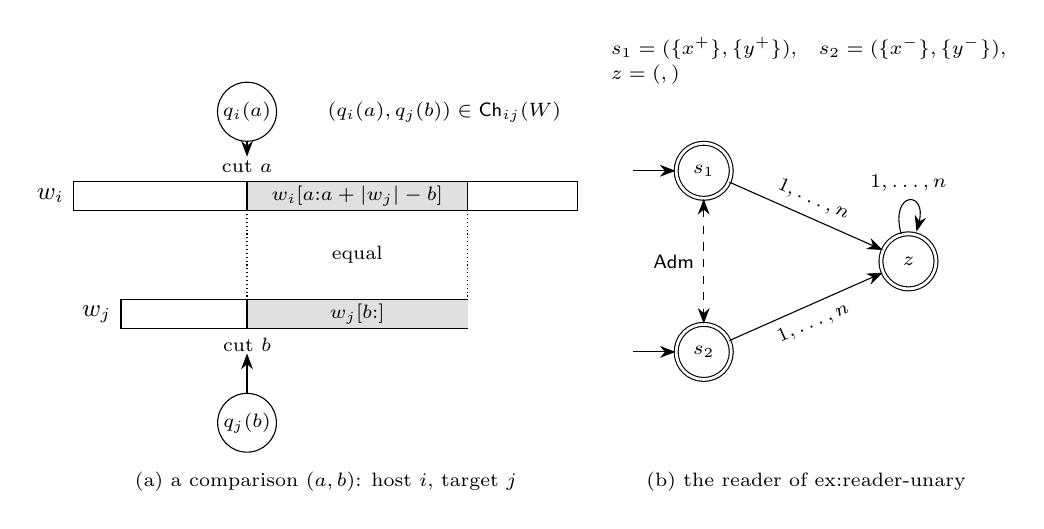
\begin{tikzpicture}[font=\small, >={Stealth[length=2mm]}]
%% Left: a channel between a host word and a target word.
\begin{scope}
  \def\h{0.36}
  % host word
  \draw (0,0) rectangle (6.4,\h);
  \fill[black!12] (2.2,0) rectangle (5.0,\h);
  \draw (2.2,0) -- (2.2,\h);
  \draw (5.0,0) -- (5.0,\h);
  \node[left] at (0,0.5*\h) {$w_i$};
  \node[above, font=\scriptsize] at (2.2,\h) {cut $a$};
  \node[font=\scriptsize] at (3.6,0.5*\h) {$\wsub{w_i}{a}{a+\len{w_j}-b}$};
  % target word
  \draw (0.6,-1.5) rectangle (5.0,-1.5+\h);
  \fill[black!12] (2.2,-1.5) rectangle (5.0,-1.5+\h);
  \draw (2.2,-1.5) -- (2.2,-1.5+\h);
  \node[left] at (0.6,-1.5+0.5*\h) {$w_j$};
  \node[below, font=\scriptsize] at (2.2,-1.5) {cut $b$};
  \node[font=\scriptsize] at (3.6,-1.5+0.5*\h) {$\wsuf{w_j}{b}$};
  \draw[densely dotted] (2.2,0) -- (2.2,-1.5+\h);
  \draw[densely dotted] (5.0,0) -- (5.0,-1.5+\h);
  \node[font=\scriptsize] at (3.6,-0.57) {equal};
  % states
  \node[circle, draw, inner sep=1pt, font=\scriptsize] (qa) at (2.2,1.25) {$q_i(a)$};
  \node[circle, draw, inner sep=1pt, font=\scriptsize] (qb) at (2.2,-2.7) {$q_j(b)$};
  \draw[->] (qa) -- (2.2,\h+0.32);
  \draw[->] (qb) -- (2.2,-1.5-0.32);
  \node[font=\scriptsize, align=left, anchor=west] at (3.1,1.25)
    {$(q_i(a),q_j(b))\in\Chan_{ij}(W)$};
  \node[font=\scriptsize, align=center] at (3.2,-3.45) {(a) a comparison $(a,b)$: host $i$, target $j$};
\end{scope}
%% Right: the reader of the worked example.
\begin{scope}[xshift=8.0cm, yshift=-0.2cm,
    st/.style={draw, circle, double, double distance=1pt, minimum size=7mm, inner sep=0pt, font=\scriptsize}]
  \node[st] (s1) at (0,0.7) {$s_1$};
  \node[st] (s2) at (0,-1.6) {$s_2$};
  \node[st] (z) at (2.6,-0.45) {$z$};
  \draw[<-] (s1) -- ++(-0.9,0);
  \draw[<-] (s2) -- ++(-0.9,0);
  \draw[->] (s1) -- node[above, sloped, font=\scriptsize] {$1,\dots,n$} (z);
  \draw[->] (s2) -- node[below, sloped, font=\scriptsize] {$1,\dots,n$} (z);
  \draw[->] (z) edge[loop above] node[font=\scriptsize] {$1,\dots,n$} (z);
  \draw[dashed, <->] (s1) -- node[left, font=\scriptsize] {$\Adm$} (s2);
  \node[font=\scriptsize, align=left, anchor=west] at (-1.3,2.1)
    {$s_1=(\{x^{\sgp}\},\{y^{\sgp}\})$,\quad $s_2=(\{x^{\sgm}\},\{y^{\sgm}\})$,\\[1pt] $z=(\varnothing,\varnothing)$};
  \node[font=\scriptsize, align=center] at (1.3,-3.25) {(b) the reader of \cref{ex:reader-unary}};
\end{scope}
\end{tikzpicture}
\caption{(a) A comparison of a tuple $W$ and its channel pair: the rest of
the target word $w_j$ after the cut $b$ is a prefix of the rest of the host
word $w_i$ after the cut $a$, and the pair of the states at the two cuts
belongs to the channel from $i$ to $j$. The tuple is a hole only if no such
pair is admitted, for all $i$ and $j$, including $i=j$. (b) The reader of
the empty constraint with the queries $(x,y)$ and $(y,x)$ in the mode vector
$(\Top,\Bot)$. All three states are rejected (double circles), the dead
state is not shown, and the admitted pairs are $(s_1,s_2)$ and
$(s_2,s_1)$.}
\label{fig:reader-hole}
\end{figure}


\subsection{The Reader of a Mode and the Reduction}\label{sec:readers-reduction}

Fix a satisfiable constraint $\Gamma$, queries $(x_1,y_1),\dots,(x_k,y_k)$
and a vector of modes $\bar\mu$, with the signed variables $p_i,p'_i$ of
\eqref{eq:seeds} and the sets $\NegV$ and $\FctV$ of \eqref{eq:neg-fct}.

\begin{definition}[The reader $M_{\bar\mu}$]\label{def:compile}
The states of $M_{\bar\mu}$ are the pairs $(P,Q)$ of sets of signed variables
with $(Q\cup\flip P)\cap\FctV=\varnothing$, where $\flip P=\{\flip r\mid r\in
P\}$, and a dead state $\dead$. The transition on a letter $i$ takes $(P,Q)$
to $(\stepU(P,i),\stepD(Q,i))$ if this pair is a state, and to $\dead$
otherwise. The $i$th start state is $(\Up(p_i,\eps),\Dn(p'_i,\eps))$ if this
pair is a state, and $\dead$ otherwise. Moreover
\begin{align*}
  (P,Q)\in\Rej&\iff P\cap\NegV=\varnothing,\\
  ((P_h,Q_h),(P_t,Q_t))\in\Adm&\iff P_t\cap(Q_h\cup\flip{P_h})\ne\varnothing.
\end{align*}
\end{definition}

Coordinate $i$ follows the upper run of its seed, in the \emph{upper
component} $P$, and the lower run of its exclusion, in the \emph{lower
component} $Q$. It dies when a prefix of
the path shows that the exclusion or the opposite of the seed lies in the
least closure, so that every solution contradicts the witness. It is
rejected when its seed derives no forbidden atom. A pair is admitted when
the seed of the target derives the exclusion of the host or the opposite of
the seed of the host, at a comparison of the two paths as in
\cref{lem:cuts}. With these readings the three conditions of
\cref{thm:realization} are exactly the conditions of a hole: \ref{it:R2} says
that no run dies, \ref{it:R1} that every endpoint is rejected, and
\ref{it:R3} that no channel contains an admitted pair.

%% guard-reader -- the two readers of the worked example with a nonempty constraint.
\begin{figure}[t]
\centering
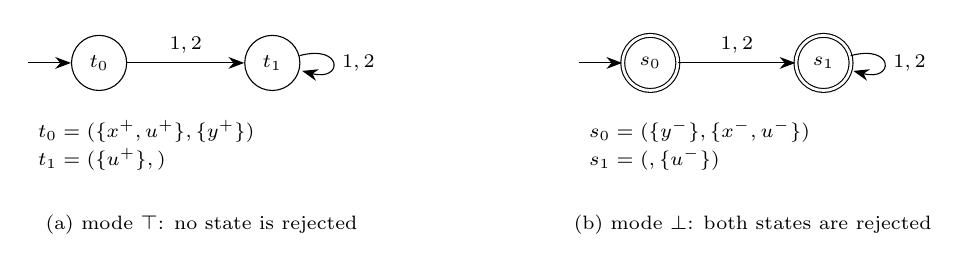
\begin{tikzpicture}[font=\scriptsize, >={Stealth[length=2mm]},
    st/.style={draw, circle, minimum size=7mm, inner sep=0pt},
    rj/.style={st, double, double distance=1pt}]
%% mode top
\begin{scope}
  \node[st] (t0) at (0,0) {$t_0$};
  \node[st] (t1) at (2.2,0) {$t_1$};
  \draw[<-] (t0) -- ++(-0.9,0);
  \draw[->] (t0) -- node[above] {$1,2$} (t1);
  \draw[->] (t1) edge[loop right] node {$1,2$} (t1);
  \node[anchor=west, align=left] at (-0.9,-1.05)
    {$t_0=(\{x^{\sgp},u^{\sgp}\},\{y^{\sgp}\})$\\[1pt] $t_1=(\{u^{\sgp}\},\varnothing)$};
  \node at (1.3,-2.05) {(a) mode $\Top$: no state is rejected};
\end{scope}
%% mode bot
\begin{scope}[xshift=7.0cm]
  \node[rj] (s0) at (0,0) {$s_0$};
  \node[rj] (s1) at (2.2,0) {$s_1$};
  \draw[<-] (s0) -- ++(-0.9,0);
  \draw[->] (s0) -- node[above] {$1,2$} (s1);
  \draw[->] (s1) edge[loop right] node {$1,2$} (s1);
  \node[anchor=west, align=left] at (-0.9,-1.05)
    {$s_0=(\{y^{\sgm}\},\{x^{\sgm},u^{\sgm}\})$\\[1pt] $s_1=(\varnothing,\{u^{\sgm}\})$};
  \node at (1.3,-2.05) {(b) mode $\Bot$: both states are rejected};
\end{scope}
\end{tikzpicture}
\caption{The readers of $\Gamma=\{u\le f(u,u),\ x\le u,\ y=\Bot\}$ and the
query $(x,y)$ (\cref{ex:guard-reader}). A state is the pair of the upper run
of the seed and the lower run of the exclusion; rejected states are drawn
with a double circle, and the dead state, which is not reachable here, is
not shown. (a) In mode $\Top$ the upper component always contains
$u^{\sgp}\in\NegV$, so there is no hole. (b) In mode $\Bot$ every word is a
hole, since no pair of states is admitted.}
\label{fig:guard-reader}
\end{figure}


\begin{theorem}[Reduction]\label{thm:reduction}
$M_{\bar\mu}$ is a structural reader over $\Dir$ with $k$ starts and at most
$2^{4\len V}+1$ states, computable from $\Gamma$, the queries and $\bar\mu$.
A tuple $W$ of paths is a hole of $M_{\bar\mu}$ if and only if some solution
of $\Gamma$ contains the seeds and none of the exclusions of $(\bar\mu,W)$.
Consequently, for a constraint $\Gamma$ that is satisfiable over $\Trees$,
\[
  \Gamma\not\entails_{\Trees}x_1\le y_1\vee\dots\vee x_k\le y_k
  \iff
  \text{$M_{\bar\mu}$ has a hole for some $\bar\mu\in\{\Top,\Bot\}^k$.}
\]
\end{theorem}

\begin{proof}[Proof sketch]
By \cref{lem:runs-det}, the state of an eligible coordinate $i$ at a cut $a$
is the pair $(\Up(p_i,\wpre{w_i}a),\Dn(p'_i,\wpre{w_i}a))$. Once $P\cap\NegV$ is empty,
the next upper set is empty, which gives \ref{it:S1} and \ref{it:S2}. A run
stays alive exactly when no prefix puts $B_i$ or $\flip{A_i}$ into the least
closure, which is \ref{it:R2}, and its endpoint is rejected exactly when
\ref{it:R1} holds. Under \ref{it:R1}, \cref{lem:cuts} states that $A_j\der
B_i$ or $A_j\der\flip{A_i}$ if and only if there are cuts $b$ of $w_j$ and
$a$ of $w_i$ with $\wsuf{w_j}b\pre\wsuf{w_i}a$ and
$\Up(p_j,\wpre{w_j}b)\cap(\Dn(p'_i,\wpre{w_i}a)\cup\Dn(\flip{p_i},\wpre{w_i}a))
\ne\varnothing$, that is, an admitted pair on the channel from $i$ to $j$.
The last statement follows with \cref{lem:witness}.
\end{proof}

\begin{example}[One query: the reader of a small constraint]\label{ex:guard-reader}
Consider the constraint $\Gamma=\{u\le f(u,u),\ x\le u,\ y=\Bot\}$ of
\cref{ex:guard-rules}, with $\NegV=\{u^{\sgp}\}$ and $\FctV=\{y^{\sgm}\}$,
and the query $(x,y)$. \Cref{fig:guard-reader} shows the two readers.

\emph{Mode $\Top$.} The seed is $(x^{\sgp},w)$ and the exclusion
$(y^{\sgp},w)$: the tree of $x$ should reach $\Top$ along $w$. The upper run
of the seed is $\Up(x^{\sgp},\eps)=\{x^{\sgp},u^{\sgp}\}$ and
$\Up(x^{\sgp},w)=\{u^{\sgp}\}$ for $w\ne\eps$, because the only way to pop
the path of the seed is to move to $u^{\sgp}$ and to pop there. No move ends
in $(y^{\sgp},w)$, so the lower run of the exclusion is $\{y^{\sgp}\}$ at
$\eps$ and empty afterwards. The upper component always contains
$u^{\sgp}\in\NegV$, so no state of the run is rejected, and the reader has
no hole: the seed always derives the forbidden atom $(u^{\sgp},\eps)$, as in
\cref{ex:guard-rules}.

\emph{Mode $\Bot$.} The seed is $(y^{\sgm},w)$ and the exclusion
$(x^{\sgm},w)$: the tree of $y$ should reach $\Bot$ along $w$ and the tree
of $x$ should not. No move starts from $y^{\sgm}$, so the upper run is
$\{y^{\sgm}\}$ at $\eps$ and empty afterwards. The lower run of the
exclusion is $\Dn(x^{\sgm},\eps)=\{x^{\sgm},u^{\sgm}\}$ and
$\Dn(x^{\sgm},w)=\{u^{\sgm}\}$ for $w\ne\eps$, since $(x^{\sgm},w)$ is
built from $(u^{\sgm},\eps)$ by pushing $w$ at $u^{\sgm}$ and moving to
$x^{\sgm}$. Both states are rejected, neither is dead, because
$y^{\sgm}\in\FctV$ belongs neither to the lower components nor to the
flipped upper components, and no pair is admitted: for the only nonempty
upper component, $\{y^{\sgm}\}\cap(\{x^{\sgm},u^{\sgm}\}\cup\{y^{\sgp}\})=
\varnothing$. So every word is a hole, in particular $w=\eps$. The hull of
its seed $(y^{\sgm},\eps)$ is the least closure, the solution $y=\Bot$,
$x=u=\fall$, and indeed $\fall\not\le\Bot$: the entailment
$\Gamma\entails x\le y$ fails.

\emph{A dead run.} For the reversed query $(y,x)$, the start state of mode
$\Top$ would be $(\{y^{\sgp}\},\{x^{\sgp}\})$, whose flipped upper component
contains the fact $y^{\sgm}$; and the start state of mode $\Bot$ would be
$(\{x^{\sgm}\},\{y^{\sgm}\})$, whose lower component contains it. So both
readers start in $\dead$ and have no hole: $\Gamma$ entails $y\le x$, as it
must, since $y=\Bot$ in every solution.
\end{example}

\begin{example}[Two queries, unary and binary]\label{ex:reader-unary}
Take the empty constraint and the queries $(x,y)$ and $(y,x)$ of
\cref{ex:unary}. There are no moves, no facts and no forbidden atoms, so
$\Up(p,\eps)=\Dn(p,\eps)=\{p\}$, both sets are empty for nonempty paths,
nothing is dead and every state is rejected. In the mode vector $(\Top,\Bot)$
the seeds are $(x^{\sgp},w_1)$ and $(x^{\sgm},w_2)$ and the exclusions
$(y^{\sgp},w_1)$ and $(y^{\sgm},w_2)$: the tree of $x$ should have a leaf of
sign $\sgp$ on $w_1$ and a leaf of sign $\sgm$ on $w_2$. The reader is shown
in \cref{fig:reader-hole}(b). The pair $(s_1,s_2)$ is admitted because the
upper component $\{x^{\sgm}\}$ of the target $s_2$ meets the flipped upper
component $\flip{\{x^{\sgp}\}}=\{x^{\sgm}\}$ of the host $s_1$, and
symmetrically for $(s_2,s_1)$.

A channel pair $(s_1,s_2)$ arises from the comparison $(0,0)$, which exists
when $w_2\pre w_1$, and $(s_2,s_1)$ when $w_1\pre w_2$. So $(w_1,w_2)$ is a hole if and only if
$w_1$ and $w_2$ are incomparable: two leaves of opposite signs cannot lie on
one path. For $n=1$ any two words are comparable and there is no hole; the
other three mode vectors give the same reader up to renaming, so the
entailment holds. For $n=2$ the tuple $(1,2)$ is a hole. The hull of its
seeds is the solution $x=f(\Top,\Bot)$, $y=\fall$ for a covariant
constructor, a countermodel.
\end{example}

\section{Small Holes: Overview}
\label{sec:overview}

By \cref{thm:reduction}, deciding a disjunctive entailment amounts to
deciding whether a structural reader has a hole. The rest of the proof is
about readers and words; it uses no property of trees or constraints, and
the alphabet $\Alp$ is arbitrary. We fix a structural reader
$M=(S,\delta,(s_i)_i,\dead,\Rej,\Adm)$ with $k$ starts and $N$ states.

\begin{theorem}[Small holes]\label{thm:small-hole}
There is a computable function $\Hole$ such that every structural reader with
$k$ starts and $N$ states that has a hole has a hole of total length at most
$\Hole(k,N)$.
\end{theorem}

The definition of $\Hole$ is given in \cref{eq:hole-bound} below, and its
growth is estimated in \cref{sec:complexity}. This section introduces the
notions that organize the proof and reduces the theorem to two bounds.

\subsection{Domination, Fresh Words and Immortal States}
\label{sec:overview-notions}

A \emph{table} with $k$ starts is the part $(S,\delta,(s_i)_i)$ of a reader:
a complete deterministic automaton with $k$ start states. Runs, endpoints and
channels of a tuple are defined for tables as in \cref{sec:readers-def}. We
write $\Vis_i(W)=\{q_i(a)\mid 0\le a\le\len{w_i}\}$ for the states that
coordinate $i$ visits.

\begin{definition}[Domination]\label{def:domination}
A tuple $U$ \emph{dominates} a tuple $W$ in a table, written $U\dominates W$,
if for all coordinates $i$ and $j$: the endpoints of coordinate $i$ in $U$
and in $W$ are equal, $\Vis_i(U)\subseteq\Vis_i(W)$, and
$\Chan_{ij}(U)\subseteq\Chan_{ij}(W)$.
\end{definition}

Domination is reflexive and transitive. A dominating tuple does nothing that
the dominated tuple does not do: it ends in the same states, passes only
through states that were already visited, and compares only pairs of states
that were already compared. Since the definition of a hole only forbids
things, we obtain:

\begin{lemma}[Holes under domination]\label{lem:hole-dominates}
If $W$ is a hole of a structural reader and $U\dominates W$ in its table,
then $U$ is a hole with the same endpoints.
\end{lemma}

\begin{proof}
The run of $u_i$ visits only states of $\Vis_i(W)$, none of which is dead,
and its endpoint is that of $w_i$, which is rejected. No pair of
$\Chan_{ij}(U)\subseteq\Chan_{ij}(W)$ is admitted.
\end{proof}

So a hole may be replaced by any tuple that dominates it, and the task is to
find short dominating tuples. The block deletions of \cref{sec:fresh} and
the compression of periodic stretches in \cref{sec:tails-compression} delete factors from the
words of a tuple in such a way that the result dominates it. The
replacement of rejected tails by rays in \cref{sec:tails-choice} is of a
different kind: it can lengthen words and change endpoints, and it only
preserves the existence of a hole. Deleting a factor between two cuts with the same state preserves endpoints
and visited states; the difficulty is always the channels, where a deletion
can bring two cuts into a comparison that did not exist before.

\begin{definition}[Fresh words]\label{def:fresh}
Coordinate $i$ of a tuple $W$ is \emph{fresh} in a table if its endpoint is
not visited earlier: $q_i(a)\ne q_i(\len{w_i})$ for every $a<\len{w_i}$. A
tuple is \emph{fresh} if all its coordinates are. A tuple $U$ \emph{freshly
dominates} $W$ if $U$ is fresh and $U\dominates W$. A fresh tuple is
\emph{minimal} if no tuple that freshly dominates it has a smaller total
length.
\end{definition}

The empty word is fresh. Since domination is transitive, every fresh tuple is
freshly dominated by a minimal fresh tuple: a fresh dominator of least total
length.

\begin{definition}[Immortal states]\label{def:immortal}
A state $q$ of a structural reader is \emph{immortal} if for every $m$ some
word of length $m$ can be read from $q$ without reaching $\dead$, and
\emph{mortal} otherwise.
\end{definition}

A state is immortal exactly when a cycle of states other than $\dead$ is
reachable from it without passing through $\dead$. Freshness comes for free
when the endpoint is mortal, and it yields the basic counting principle of
the whole proof: \emph{cuts at which comparable rests begin carry different
states}.

\begin{lemma}[Distinct states]\label{lem:distinct}
Let $W$ be a tuple and $a<b$ cuts of $w_i$ such that
$\wsuf{w_i}b\pre\wsuf{w_i}a$.
\begin{enumerate}
\item\label{it:distinct-fresh} If coordinate $i$ is fresh, then
  $q_i(a)\ne q_i(b)$.
\item\label{it:distinct-mortal} If coordinate $i$ is eligible with a mortal
  endpoint, then it is fresh.
\item\label{it:distinct-head} If coordinate $i$ is eligible and
  $b\le J_i$, then $q_i(a)\ne q_i(b)$.
\end{enumerate}
\end{lemma}

\begin{proof}
(1) If $q_i(a)=q_i(b)$, reading $\wsuf{w_i}b$ from the cut $a$ leads to the
endpoint, at the cut $a+\len{w_i}-b<\len{w_i}$. (2) If the endpoint occurs at
a cut $a<\len{w_i}$, the run from $a$ to the end is a cycle of states other
than $\dead$, so the endpoint is immortal. (3) If $q_i(a)=q_i(b)$, reading
$\wsub{w_i}b{J_i}$ from the cut $a$ leads to the rejected state $q_i(J_i)$ at
the cut $a+J_i-b<J_i$, before the first rejected cut.
\end{proof}

In particular, a fixed text has fewer than $N$ nonempty rests of one fresh
word as prefixes, since these rests are comparable.

\subsection{The Two Bounds}\label{sec:overview-bounds}

The first bound concerns the coordinates with immortal endpoints. Recall that
the rejected tail of an eligible coordinate is the part of its word after
the first rejected cut.

\begin{theorem}[Rejected tails]\label{thm:tails}
There is a computable function $\TailB$ such that every structural reader
with $k$ starts and $N$ states that has a hole has a hole in which the
rejected tail of every coordinate with an immortal endpoint has length at
most $\TailB(k,N)$.
\end{theorem}

The second bound is a statement about tables, which have no rejected states,
no dead state and no admitted pairs.

\begin{theorem}[Fresh tuples]\label{thm:fresh}
There is a computable function $\FreshB$ such that every minimal fresh tuple
of a table with $k$ starts and $N$ states has total length at most
$\FreshB(k,N)$. Hence every fresh tuple is freshly dominated by a tuple of
total length at most $\FreshB(k,N)$.
\end{theorem}

Neither bound depends on the size of the alphabet. \Cref{thm:fresh} is proved
in \cref{sec:fresh} and \cref{thm:tails} in \cref{sec:tails}.

Why two bounds? A hole need not be fresh: a coordinate with an immortal
endpoint may run through its endpoint many times. Deleting such a loop is
tempting, but it changes the rests of the word after all earlier cuts, and
with them the channels in which this coordinate is the host. For a
coordinate with a mortal endpoint the situation is rigid, by
\cref{lem:distinct}. \Cref{thm:tails} is the tool that brings immortal
coordinates under control: once the rejected tail is short, the coordinate
can be made fresh in a larger table that counts the letters of the tail.

\subsection{The Cover of a Hole}\label{sec:overview-cover}

%% cover -- the cover of a hole on a tracked coordinate.
\begin{figure}[t]
\centering
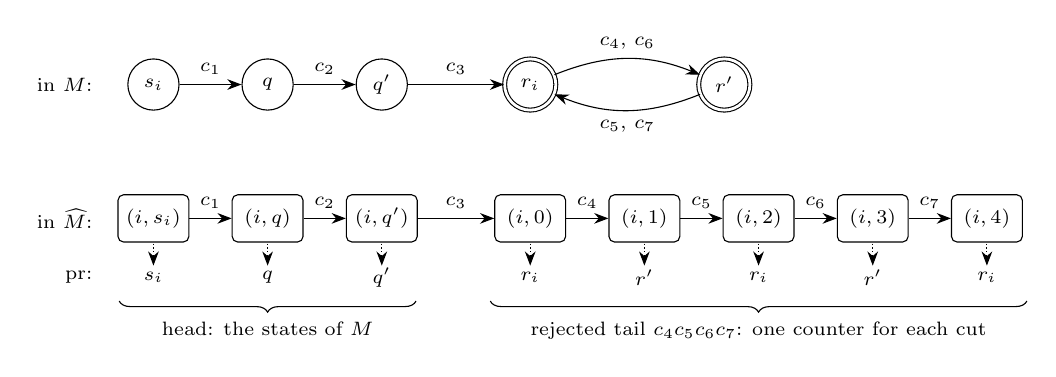
\begin{tikzpicture}[font=\scriptsize, >={Stealth[length=1.8mm]}, x=1.45cm, y=1cm,
    st/.style={draw, circle, minimum size=6.5mm, inner sep=0pt},
    rj/.style={st, double, double distance=1pt},
    cv/.style={draw, rounded corners=2pt, minimum height=6mm, minimum width=9mm, inner sep=1.5pt}]
%% the run in M
\node[st] (m0) at (0,0) {$s_i$};
\node[st] (m1) at (1,0) {$q$};
\node[st] (m2) at (2,0) {$q'$};
\node[rj] (m3) at (3.3,0) {$r_i$};
\node[rj] (m4) at (5.0,0) {$r'$};
\draw[->] (m0) -- node[above] {$c_1$} (m1);
\draw[->] (m1) -- node[above] {$c_2$} (m2);
\draw[->] (m2) -- node[above] {$c_3$} (m3);
\draw[->] (m3) to[bend left=22] node[above] {$c_4,\,c_6$} (m4);
\draw[->] (m4) to[bend left=22] node[below] {$c_5,\,c_7$} (m3);
\node[left] at (-0.45,0) {in $M$:};
%% the run in the cover
\node[cv] (c0) at (0,-1.7) {$(i,s_i)$};
\node[cv] (c1) at (1,-1.7) {$(i,q)$};
\node[cv] (c2) at (2,-1.7) {$(i,q')$};
\node[cv] (c3) at (3.3,-1.7) {$(i,0)$};
\node[cv] (c4) at (4.3,-1.7) {$(i,1)$};
\node[cv] (c5) at (5.3,-1.7) {$(i,2)$};
\node[cv] (c6) at (6.3,-1.7) {$(i,3)$};
\node[cv] (c7) at (7.3,-1.7) {$(i,4)$};
\draw[->] (c0) -- node[above] {$c_1$} (c1);
\draw[->] (c1) -- node[above] {$c_2$} (c2);
\draw[->] (c2) -- node[above] {$c_3$} (c3);
\draw[->] (c3) -- node[above] {$c_4$} (c4);
\draw[->] (c4) -- node[above] {$c_5$} (c5);
\draw[->] (c5) -- node[above] {$c_6$} (c6);
\draw[->] (c6) -- node[above] {$c_7$} (c7);
\node[left] at (-0.45,-1.7) {in $\cov M$:};
%% projection
\node[left] at (-0.45,-2.45) {$\proj$:};
\foreach \x/\l in {0/s_i,1/q,2/q',3.3/r_i,4.3/r',5.3/r_i,6.3/r',7.3/r_i} { \node at (\x,-2.45) {$\l$}; }
\foreach \x in {0,1,2,3.3,4.3,5.3,6.3,7.3} { \draw[densely dotted, ->] (\x,-2.02) -- (\x,-2.3); }
\draw[decorate, decoration={brace, mirror, amplitude=4pt}] (-0.3,-2.75) -- (2.3,-2.75)
  node[midway, below=4pt] {head: the states of $M$};
\draw[decorate, decoration={brace, mirror, amplitude=4pt}] (2.95,-2.75) -- (7.65,-2.75)
  node[midway, below=4pt] {rejected tail $c_4c_5c_6c_7$: one counter for each cut};
\end{tikzpicture}
\caption{The cover on a tracked coordinate $i$ with $w_i=c_1\cdots c_7$,
$J_i=3$ and $\ell_i=4$. In $M$ the rejected tail runs twice through the
cycle of the rejected states $r_i$ and $r'$, so the endpoint $r_i$ is
visited three times and the word is not fresh. In the cover the tail is
spelled out by the counters $(i,0),\dots,(i,4)$, the endpoint $(i,4)$ is
visited once. From each displayed counter, every transition other than the
displayed next-letter transition leads to the absorbing state $o$, and all
transitions from $(i,4)$ lead to $o$; other transitions from copies of head
states follow \cref{def:cover-hole}. On the displayed run, the projection $\proj$
(last row) maps each state to the state of $M$ at the same cut.}
\label{fig:cover}
\end{figure}


A hole whose immortal tails are short is not yet fresh, but it becomes fresh
in a larger table that counts the letters of these tails
(\cref{fig:cover}). Let $W$ be a hole of $M$ and $L$ a number such that
every coordinate with an immortal endpoint has a rejected tail of length at
most $L$. Call a coordinate $i$ \emph{tracked} if its rejected tail has
length $\ell_i=\len{w_i}-J_i\le L$; the other coordinates have mortal
endpoints.

\begin{definition}[Cover of a hole]\label{def:cover-hole}
The \emph{cover} $\cov M$ of $W$ is the following table with $k$ starts. Its
states are an absorbing state $o$ and, for each coordinate $i$, the pairs
$(i,s)$ with $s\in S$ and the \emph{counters} $(i,m)$ with $0\le m\le L$,
all of them distinct.
\begin{itemize}
\item For an untracked coordinate $i$, the start is $(i,s_i)$ and a letter
  $c$ takes $(i,s)$ to $(i,\delta(s,c))$.
\item For a tracked coordinate $i$ with first rejected state
  $r_i=q_i(J_i)$, a letter $c$ takes $(i,s)$ with $s\notin\Rej$ to the
  counter $(i,0)$ if $\delta(s,c)=r_i$, to $(i,\delta(s,c))$ if
  $\delta(s,c)\notin\Rej$, and to $o$ otherwise. It takes a counter $(i,m)$
  with $m<\ell_i$ to $(i,m+1)$ if $c$ is the letter of $w_i$ at the
  position $J_i+m$, and to $o$ otherwise; since $\ell_i\le L$, the counter
  $(i,m+1)$ exists. The start is $(i,0)$ if $J_i=0$ and $(i,s_i)$
  otherwise.
\item All remaining transitions lead to $o$. In particular, so do all
  transitions from the counter $(i,\ell_i)$ of a tracked coordinate and
  from the counters of an untracked one.
\end{itemize}
The \emph{projection} $\proj$ maps $(i,s)$ to $s$, the counter $(i,m)$ of a
tracked coordinate with $m\le\ell_i$ to $q_i(J_i+m)$, and all other counters
and $o$ to $\dead$.
\end{definition}

So the cover follows $M$ on the head of a tracked word and then spells out
its rejected tail, letter by letter. It has $k(N+L+1)+1$ states.

\begin{lemma}[Cover]\label{lem:cover}
The tuple $W$ is fresh in its cover $\cov M$, and every tuple that dominates
$W$ in $\cov M$ is a hole of $M$ with the same endpoints as $W$.
\end{lemma}

\begin{proof}
On a tracked coordinate $i$, the run of $w_i$ in the cover is $(i,q_i(a))$
at the cuts $a<J_i$ and the counter $(i,a-J_i)$ at the cuts $a\ge J_i$; on an
untracked coordinate it is $(i,q_i(a))$. In the first case the endpoint is
the counter $(i,\ell_i)$, which occurs only at the last cut. In the
second case the endpoint of $w_i$ in $M$ is mortal, so coordinate $i$ is
fresh in $M$ by \cref{lem:distinct}, hence in the cover. So $W$ is fresh in
the cover, and its runs avoid $o$.

Whenever a transition of the cover from a state $z$ on a letter $c$ does not
lead to $o$, it leads to a state with projection $\delta(\proj(z),c)$; this is
checked case by case, and for a counter it holds because the letter read is
the letter of $w_i$. The starts project to the starts of $M$. Now let $U$
dominate $W$ in the cover. The runs of $U$ in the cover visit only states
visited by $W$, so they avoid $o$, and therefore the run of $U$ in $M$ is the
projection of its run in the cover. Applying $\proj$ to the three conditions of
domination in the cover gives $U\dominates W$ in the table of $M$, because
the run of $W$ in $M$ is also the projection of its run in the cover. By
\cref{lem:hole-dominates}, $U$ is a hole of $M$ with the endpoints of $W$.
\end{proof}

\begin{proof}[Proof of \cref{thm:small-hole} from
\cref{thm:tails,thm:fresh}]
Let $M$ have a hole. By \cref{thm:tails} it has a hole $W$ whose coordinates
with immortal endpoints have rejected tails of length at most
$L=\TailB(k,N)$. By \cref{lem:cover}, $W$ is fresh in its cover, a table with
$k$ starts and $k(N+L+1)+1$ states, so by \cref{thm:fresh} it is freshly
dominated there by a tuple $U$ of total length at most
\begin{equation}\label{eq:hole-bound}
  \Hole(k,N)=\FreshB\bigl(k,\;k\,(N+\TailB(k,N)+1)+1\bigr).
\end{equation}
By \cref{lem:cover} again, $U$ is a hole of $M$.
\end{proof}

The composition explains the shape of the final bound: the fresh-tuple bound
is applied to a table whose size is the rejected-tail bound. For each fixed
number $k$ of starts, both are doubly exponential in $N$
(\cref{thm:elementary}), which gives four iterated exponentials in $N$.

\section{Fresh Tuples}
\label{sec:fresh}

This section explains the proof of \cref{thm:fresh}: a minimal fresh tuple
of a table with $k$ starts and $N$ states has bounded total length. We fix
such a table and a fresh tuple $W=(w_1,\dots,w_k)$. Full proofs are in
\cref{app:fresh}.

\subsection{The Idea}\label{sec:fresh-idea}

To shorten $W$ we delete a factor between two cuts of one word that carry
the same state. This preserves endpoints and visited states, but in general
not the channels. A channel compares the rest of a target word with a factor
of a host word. If we delete a factor from the host in the middle of such a
comparison, the two sides no longer match; and after the deletion the rest
of some word may match a factor of the edited host that it did not match
before, at cuts whose states were never compared. Both effects disappear if
the deletion is \emph{invisible to every comparison}: whenever a comparison
runs over a deleted factor on one side, the same factor is deleted at the
corresponding place on the other side.

This suggests deleting a repeated factor at \emph{all} places that look
alike, in all words at once. The question is what ``look alike'' should
mean. Comparing bounded windows of letters is not enough, because a
comparison can run over arbitrarily long equal texts. We therefore cut all
words into blocks by a rule that depends only on the text, so that equal
texts are cut in the same way, up to a bounded number of blocks at their left
ends. The cutting rule is given by \emph{markers}, suffixes of the words
$w_i$ themselves, and it is iterated: the blocks of one level are grouped
into the blocks of the next level, until every word is a single block.
Deleting equal stretches of blocks at equal distances from the right ends of
equal block sequences is then invisible to comparisons, and a pigeonhole
argument finds such stretches whenever some block consists of too many
blocks of the level below.

\subsection{The Marker Hierarchy}\label{sec:fresh-hierarchy}

\begin{definition}[Markers and anchors]\label{def:markers}
For each \emph{level} $t\ge1$ we define a set $\Act_t$ of \emph{active}
coordinates and, for $l\in\Act_t$, a \emph{marker} $\mk tl$, a nonempty
suffix of $w_l$.
\begin{itemize}
\item $\Act_1$ consists of the coordinates with a nonempty word, and $\mk 1l$
  is the last letter of $w_l$.
\item A \emph{level-$t$ anchor} of a text $u$ is a cut $e\ge1$ of $u$ at
  which $\mk tm$ ends, for some $m\in\Act_t$. The level-$t$ anchors of the
  word $w_l$ are its anchors as a text together with its end $\len{w_l}$.
\item A coordinate $l\in\Act_t$ belongs to $\Act_{t+1}$ if $w_l$ has a
  level-$t$ anchor $e<\len{w_l}$. Let $e$ be the last such anchor and
  $\mk tm$ the longest level-$t$ marker that ends at $e$. Then
  $\mk{t+1}l=\wsuf{w_l}{e-\len{\mk tm}}$.
\end{itemize}
The \emph{level-$0$ anchors} of a text are all its cuts $e\ge1$. The
level-$t$ anchors cut each nonempty word into its \emph{level-$t$ blocks},
the factors between consecutive anchors, the first block beginning at the
cut $0$. The \emph{top level} is the largest $t$ with $\Act_t\ne\varnothing$,
and $0$ if all words are empty.
\end{definition}

%% markers -- the marker hierarchy of the running example.
\begin{figure}[t]
\centering
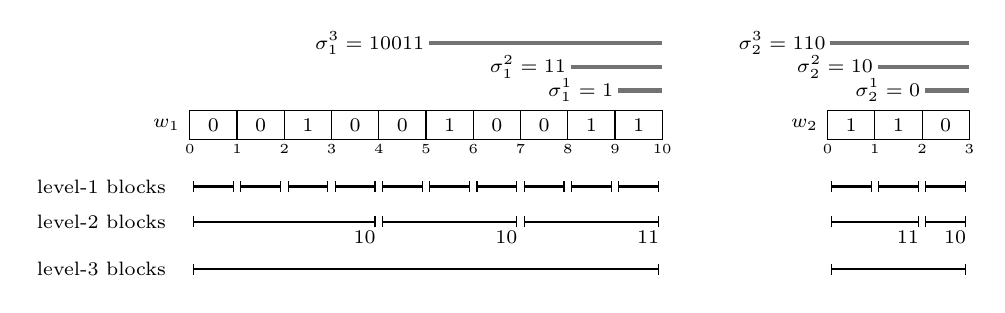
\begin{tikzpicture}[font=\scriptsize, x=0.6cm, y=1cm]
\def\h{0.36}
%% #1 x-offset, #2 list of letters
\newcommand{\letters}[2]{%
  \foreach \c [count=\i from 0] in {#2} {
    \draw (#1+\i,0) rectangle (#1+\i+1,\h);
    \node at (#1+\i+0.5,0.5*\h) {$\c$};
  }}
%% a block row: #1 y, #2 x-offset, #3 list of cuts a/b
\newcommand{\blockrow}[3]{%
  \foreach \a/\b in {#3} {
    \draw[line width=0.9pt] (#2+\a+0.08,#1) -- (#2+\b-0.08,#1);
    \draw (#2+\a+0.08,#1-0.07) -- (#2+\a+0.08,#1+0.07);
    \draw (#2+\b-0.08,#1-0.07) -- (#2+\b-0.08,#1+0.07);
  }}
%% a marker above the word: #1 height, #2 x-offset, #3 from, #4 to, #5 label
\newcommand{\marker}[5]{%
  \draw[line width=1.5pt, black!55] (#2+#3+0.06,#1) -- (#2+#4,#1);
  \node[left, inner sep=1.5pt] at (#2+#3+0.06,#1) {#5};}
%% w1
\letters{0}{0,0,1,0,0,1,0,0,1,1}
\node[left] at (0,0.5*\h) {$w_1$};
\foreach \i in {0,...,10} { \node[below, font=\tiny, inner sep=1pt] at (\i,-0.02) {$\i$}; }
\marker{0.62}{0}{9}{10}{$\mk11=1$}
\marker{0.92}{0}{8}{10}{$\mk21=11$}
\marker{1.22}{0}{5}{10}{$\mk31=10011$}
\blockrow{-0.6}{0}{0/1,1/2,2/3,3/4,4/5,5/6,6/7,7/8,8/9,9/10}
\blockrow{-1.05}{0}{0/4,4/7,7/10}
\blockrow{-1.65}{0}{0/10}
\node[left] at (-0.3,-0.6) {level-$1$ blocks};
\node[left] at (-0.3,-1.05) {level-$2$ blocks};
\node[left] at (-0.3,-1.65) {level-$3$ blocks};
\foreach \x/\m in {4/10,7/10,10/11} { \node[below, inner sep=1pt] at (\x-0.3,-1.12) {$\m$}; }
%% w2
\letters{13.5}{1,1,0}
\node[left] at (13.5,0.5*\h) {$w_2$};
\foreach \i in {0,...,3} { \node[below, font=\tiny, inner sep=1pt] at (13.5+\i,-0.02) {$\i$}; }
\marker{0.62}{13.5}{2}{3}{$\mk12=0$}
\marker{0.92}{13.5}{1}{3}{$\mk22=10$}
\marker{1.22}{13.5}{0}{3}{$\mk32=110$}
\blockrow{-0.6}{13.5}{0/1,1/2,2/3}
\blockrow{-1.05}{13.5}{0/2,2/3}
\blockrow{-1.65}{13.5}{0/3}
\foreach \x/\m in {2/11,3/10} { \node[below, inner sep=1pt] at (13.5+\x-0.3,-1.12) {$\m$}; }
\end{tikzpicture}
\caption{The marker hierarchy of \cref{ex:hierarchy}. Above each word: its
markers of the levels $1$, $2$, $3$, nested suffixes of the word. Below: the
blocks of each level; a block ends where a marker of that level ends, in any
of the words. Under each level-$2$ block the level-$2$ marker that ends
there is shown: $10$ ends at the cuts $4$ and $7$ of $w_1$ and at the end of
$w_2$, and $11$ ends at the end of $w_1$ and at the cut $2$ of $w_2$.}
\label{fig:markers}
\end{figure}


So the blocks of level $0$ are single letters, the blocks of level $1$ end
with the last letter of some word, and the marker of the next level consists
of the last block of the word together with the marker in front of it. A
coordinate stops being active when its word is a single block.

\begin{example}\label{ex:hierarchy}
Let $W=(w_1,w_2)$ with $w_1=0010010011$ and $w_2=110$
(\cref{fig:markers}). The level-$1$
markers are the letters $1$ and $0$, so every cut is a level-$1$ anchor and
the level-$1$ blocks are single letters. In $w_1$ the last anchor before the
end is the cut $9$, where the marker $1$ ends, so $\mk21=11$; in $w_2$ it is
the cut $2$, and $\mk22=10$. The level-$2$ anchors are the cuts at which $11$
or $10$ ends: the cuts $4$, $7$ and $10$ of $w_1$, and the cuts $2$ and $3$
of $w_2$. They cut the words into the level-$2$ blocks
\[
  w_1=0010\cdot010\cdot011,\qquad w_2=11\cdot0 .
\]
At level $3$ the markers are $\mk31=10\,011$ (the level-$2$ marker $10$ that
ends at the cut $7$, followed by the last block) and $\mk32=11\,0=w_2$.
Neither occurs at another place, so the level-$3$ blocks are the whole words,
no coordinate is active at level $4$, and the top level is $3$.
\end{example}

The hierarchy has three structural properties. The first is the reason why
blocks behave well under comparisons.

\begin{lemma}[Markers]\label{lem:markers}
For every level $t\ge1$:
\begin{enumerate}
\item\label{it:mk-anti} \emph{Factor antichain.} If $l,m\in\Act_t$ and
  $\mk tl$ is a factor of $\mk tm$, then $\mk tl=\mk tm$. Consequently, if an
  occurrence of an active level-$t$ marker in a text lies inside an
  occurrence of another one, the two occurrences coincide.
\item\label{it:mk-two} For $l\in\Act_{t+1}$, the marker $\mk tl$ is a proper
  suffix of $\mk{t+1}l$, and the text $\mk{t+1}l$ has exactly two level-$t$
  anchors: the end of the level-$t$ marker it begins with, and its own end.
\item\label{it:mk-nest} Every level-$(t+1)$ anchor of a text is a level-$t$
  anchor of it.
\end{enumerate}
\end{lemma}

By \eqref{it:mk-nest} the blocks of level $t+1$ are concatenations of blocks
of level $t$. The freshness of $W$ enters through \cref{lem:distinct}: a
fixed text has at most $N-1$ nonempty rests of one word $w_l$ as prefixes.

\begin{lemma}[Depth and span]\label{lem:depth-span}
\begin{enumerate}
\item\label{it:depth} The top level is at most $k(N-1)$.
\item\label{it:span} In every text, an occurrence $\wsub uab$ of a
  level-$(t+1)$ marker contains at most $k(N-1)+2$ level-$t$ anchors $e$ of
  $u$ with $a<e\le b$.
\end{enumerate}
\end{lemma}

For \eqref{it:depth}, a marker of level $t$ has at least $t$ prefixes that
are suffixes of words, namely the markers nested at its left end, and these
give rests of words that are prefixes of one text. For \eqref{it:span}, a
level-$t$ marker that ends inside the occurrence lies inside it, which
happens at two anchors by \cref{lem:markers}, or it begins to the left of
it, and then the part inside is a rest of a word and a prefix of the marker.

\subsection{Parses and the Reverse Trie}\label{sec:fresh-trie}

Fix a level $t$ between $0$ and the top level. We call the blocks of level
$t+1$ \emph{upper blocks} and those of level $t$ \emph{lower blocks}; at the
top level the upper blocks are the nonempty words. An \emph{upper occurrence}
is an upper block together with its place, a word and two cuts. Its
\emph{parse} is the sequence of its lower blocks, a word over the alphabet of
lower blocks, and for $d\ge0$ its \emph{cut at depth $d$} is the cut that
lies $d$ lower blocks to the left of its end.

Equal texts are parsed alike only up to their left ends: a marker that
begins before an upper block can end inside it and create an additional
anchor there. Different occurrences of one text can therefore have different
parses, but by \cref{lem:distinct} only at boundedly many places, all to the
left of the first anchor that the text has on its own
(\cref{lem:parse-local}). What matters is how parses end. For two parses $Z$
and $Y$ let $\lcsuf(Z,Y)$ be the number of lower blocks in their longest
common suffix.

\begin{definition}[Reverse trie]\label{def:trie}
The \emph{nodes} on the path of a parse $Z$ are $0$, the length of $Z$, and
the numbers $\lcsuf(Z,Y)$ for the parses $Y$ of all upper occurrences. An
\emph{edge} is a parse $Z$ with two consecutive nodes $a<b$ on its path. An
upper occurrence \emph{traverses} the edge if its parse $Y$ satisfies
$\lcsuf(Y,Z)\ge b$.
\end{definition}

This is the trie of all parses read from the right; an edge is a stretch of
a parse along which no other parse branches off. All upper occurrences that
traverse an edge end with the same $b$ lower blocks, and whether an
occurrence traverses the edge is decided by a bounded part of the text at
its right end (\cref{lem:traverse}).

\begin{example}\label{ex:trie}
In \cref{ex:hierarchy} take $t=1$. The lower blocks are the letters, and the
upper blocks are the level-$2$ blocks $0010$, $010$, $011$ of $w_1$ and
$11$, $0$ of $w_2$; the parse of an upper block is the sequence of its
letters. For $Z=0010$ we have $\lcsuf(Z,010)=3$, $\lcsuf(Z,0)=1$ and
$\lcsuf(Z,011)=\lcsuf(Z,11)=0$. So the nodes on the path of $Z$ are
$0,1,3,4$, and its edges are $(Z,0,1)$, $(Z,1,3)$ and $(Z,3,4)$
(\cref{fig:trie}). The edge $(Z,1,3)$ is traversed by the upper blocks
$0010$ and $010$ of $w_1$, which end with the same three lower blocks
$0,1,0$; the edge $(Z,0,1)$ is traversed by these two and by the upper block
$0$ of $w_2$. The upper block $010$ lies between the cuts $4$ and $7$ of
$w_1$, and its cuts at the depths $0,1,2,3$ are $7,6,5,4$.
\end{example}

%% trie -- the reverse trie of the running example at level 1.
\begin{figure}[t]
\centering
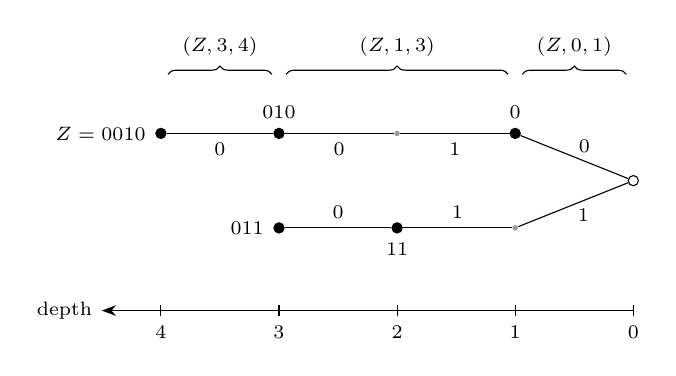
\begin{tikzpicture}[font=\scriptsize, x=1.5cm, y=1cm,
    nd/.style={circle, draw, fill=white, inner sep=1.3pt},
    en/.style={circle, draw, fill=black, inner sep=1.3pt},
    pt/.style={circle, fill=black!40, inner sep=0.7pt}]
%% depth d is drawn at x = -d; root at the right
\node[nd] (r) at (0,0) {};
%% branch ending with 0: parses 0, 010, 0010
\node[en] (a1) at (-1,0.6) {};
\node[pt] (a2) at (-2,0.6) {};
\node[en] (a3) at (-3,0.6) {};
\node[en] (a4) at (-4,0.6) {};
\draw (r) -- node[above right, inner sep=1.5pt] {$0$} (a1);
\draw (a1) -- node[below] {$1$} (a2);
\draw (a2) -- node[below] {$0$} (a3);
\draw (a3) -- node[below] {$0$} (a4);
\node[above=2pt] at (a1) {$0$};
\node[above=2pt] at (a3) {$010$};
\node[left=2pt] at (a4) {$Z=0010$};
%% branch ending with 1: parses 11, 011
\node[pt] (b1) at (-1,-0.6) {};
\node[en] (b2) at (-2,-0.6) {};
\node[en] (b3) at (-3,-0.6) {};
\draw (r) -- node[below right, inner sep=1.5pt] {$1$} (b1);
\draw (b1) -- node[above] {$1$} (b2);
\draw (b2) -- node[above] {$0$} (b3);
\node[below=2pt] at (b2) {$11$};
\node[left=2pt] at (b3) {$011$};
%% edges of the path of Z
\foreach \a/\b/\l in {0/1/{(Z,0,1)},1/3/{(Z,1,3)},3/4/{(Z,3,4)}} {
  \draw[decorate, decoration={brace, amplitude=3pt}] (-\b+0.06,1.35) -- (-\a-0.06,1.35)
    node[midway, above=3pt] {$\l$};
}
%% depth axis
\draw[->, >={Stealth[length=1.8mm]}] (0,-1.65) -- (-4.5,-1.65) node[left] {depth};
\foreach \d in {0,...,4} { \draw (-\d,-1.58) -- (-\d,-1.72) node[below] {$\d$}; }
\end{tikzpicture}
\caption{The reverse trie of \cref{ex:trie}: the parses of the five upper
blocks, read from the right; the edges of the drawing are labeled with
lower blocks, here letters. A black node is the end of the parse written
next to it. The path of
$Z=0010$ has the nodes $0,1,3,4$; nothing branches off at depth $2$, so
$(Z,1,3)$ is one edge, which is traversed by the upper blocks $0010$ and
$010$.}
\label{fig:trie}
\end{figure}


\subsection{Block Deletions}\label{sec:fresh-deletion}

For a cut $c$ of a word $w_l$, let $\tau_r(l,c)$ be the text of the
level-$r$ marker that ends at $c$, if there is one; it is unique by
\cref{lem:markers}. Let $\omega(l,c)$ be the largest length of these texts
for $1\le r\le t$, and $0$ if there are none. The \emph{label} of the cut is
\[
  \lab(l,c)=\bigl(\tau_1(l,c),\dots,\tau_t(l,c),\;q_l(c-\omega(l,c))\bigr):
\]
the markers of all levels up to $t$ that end at the cut, and the state
before the longest of them. Two cuts of one word with equal labels have the
same $\omega$ letters to their left and the same states at all distances up
to $\omega$, in particular the same state. In \cref{ex:hierarchy} with
$t=2$, the markers $0$ of level $1$ and $10$ of level $2$ end at the cut $7$
of $w_1$, so $\omega(1,7)=2$ and $\lab(1,7)=(0,\,10,\,q_1(5))$; likewise
$\lab(1,4)=(0,\,10,\,q_1(2))$. The two labels are equal exactly when
$q_1(2)=q_1(5)$, and then also $q_1(3)=q_1(6)$ and $q_1(4)=q_1(7)$, because
the same letters $1,0$ are read from equal states.

Deletions will be restricted to the interior of an edge. The \emph{margin}
\[
  \Marg=3kN-k+5
\]
is the number of lower blocks that are kept free at both ends of the edge.
At the end $b$, where the parses branch, the margin ensures that the markers
ending at the cuts in question lie inside the text that all traversing
occurrences share, so that their labels can be compared
(\cref{lem:labels-local}). At the end $a$ it leaves enough common lower
blocks to the right of a deleted factor to recognize, from the text alone,
every upper block that traverses the edge (\cref{lem:traverse}).

\begin{definition}[Block deletion]\label{def:block-deletion}
A \emph{block deletion} at level $t$ consists of an edge $(Z,a,b)$ and two
depths $i<j$ with $a+\Marg\le i$ and $j\le b-\Marg$ such that, in every upper
occurrence $o$ that traverses the edge, the cuts of $o$ at the depths $j$ and
$i$ have equal labels. It deletes, from every traversing upper occurrence,
the factor between its cuts at the depths $j$ and $i$.
\end{definition}

\Cref{fig:hierarchy} illustrates the definition. The deleted factors are
equal words, since traversing occurrences end with the same $b$ lower
blocks, and at least one factor is deleted. The words of the example are
far too short for a block deletion, since an edge must have more than
$2\Marg$ lower blocks; in general, deletions exist as soon as some edge is
long (\cref{sec:fresh-bound}).

%% hierarchy -- a block deletion along an edge of the reverse trie, before and after.
\begin{figure}[t]
\centering
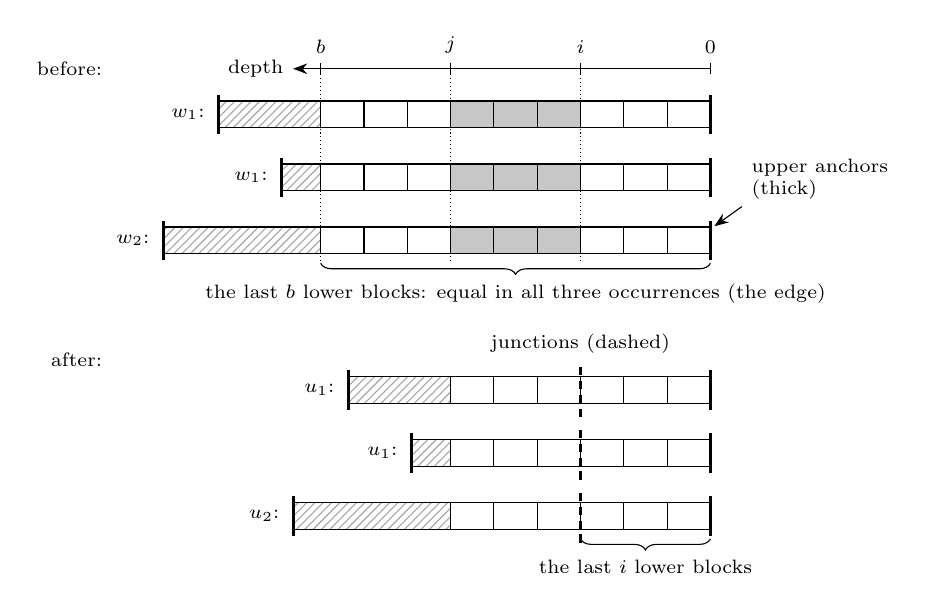
\begin{tikzpicture}[font=\scriptsize, >={Stealth[length=1.8mm]}]
\def\h{0.34}
%% draws an upper block ending at x=#1, y=#2, with a context-dependent left part of width #3
\newcommand{\upperblock}[4]{%
  % common suffix: blocks of depths 0..b-1 (b = 9 lower blocks of width .55)
  \foreach \d in {0,...,8} {
    \pgfmathsetmacro{\xr}{#1-0.55*\d}
    \pgfmathsetmacro{\xl}{#1-0.55*(\d+1)}
    \ifnum\d>2 \ifnum\d<6
      \fill[black!22] (\xl,#2) rectangle (\xr,#2+\h);
    \fi\fi
    \draw (\xl,#2) rectangle (\xr,#2+\h);
  }
  % the part above the edge, different in each occurrence
  \pgfmathsetmacro{\xe}{#1-0.55*9}
  \draw[pattern=north east lines, pattern color=black!35] (\xe-#3,#2) rectangle (\xe,#2+\h);
  \draw[line width=1.1pt] (#1,#2-0.08) -- (#1,#2+\h+0.08);
  \draw[line width=1.1pt] (\xe-#3,#2-0.08) -- (\xe-#3,#2+\h+0.08);
  \node[left] at (\xe-#3-0.05,#2+0.5*\h) {#4};
}
%% the same upper block after the deletion: 6 lower blocks of the edge remain
\newcommand{\upperblockafter}[4]{%
  \foreach \d in {0,...,5} {
    \pgfmathsetmacro{\xr}{#1-0.55*\d}
    \pgfmathsetmacro{\xl}{#1-0.55*(\d+1)}
    \draw (\xl,#2) rectangle (\xr,#2+\h);
  }
  \pgfmathsetmacro{\xe}{#1-0.55*6}
  \pgfmathsetmacro{\xj}{#1-0.55*3}
  \draw[pattern=north east lines, pattern color=black!35] (\xe-#3,#2) rectangle (\xe,#2+\h);
  \draw[line width=1.1pt] (#1,#2-0.08) -- (#1,#2+\h+0.08);
  \draw[line width=1.1pt] (\xe-#3,#2-0.08) -- (\xe-#3,#2+\h+0.08);
  \draw[line width=1.3pt, densely dashed] (\xj,#2-0.17) -- (\xj,#2+\h+0.17);
  \node[left] at (\xe-#3-0.05,#2+0.5*\h) {#4};
}
\upperblock{9.2}{2.0}{1.3}{$w_1$:}
\upperblock{9.2}{1.2}{0.5}{$w_1$:}
\upperblock{9.2}{0.4}{2.0}{$w_2$:}
%% depth scale
\draw[->] (9.2,2.75) -- (3.9,2.75) node[left] {depth};
\foreach \d/\l in {0/0,3/i,6/j,9/b} {
  \pgfmathsetmacro{\x}{9.2-0.55*\d}
  \draw (\x,2.68) -- (\x,2.82) node[above] {$\l$};
}
\draw[densely dotted] (9.2-0.55*3,2.68) -- (9.2-0.55*3,0.3);
\draw[densely dotted] (9.2-0.55*6,2.68) -- (9.2-0.55*6,0.3);
\draw[densely dotted] (9.2-0.55*9,2.68) -- (9.2-0.55*9,0.3);
\draw[decorate, decoration={brace, mirror, amplitude=4pt}] (9.2-0.55*9,0.28) -- (9.2,0.28)
  node[midway, below=4pt] {the last $b$ lower blocks: equal in all three occurrences (the edge)};
\node[align=left, anchor=west] at (9.6,1.35) {upper anchors\\ (thick)};
\draw[->] (9.6,1.0) -- (9.25,0.75);
\node[anchor=east] at (1.6,2.75) {before:};
%% after the deletion
\begin{scope}[yshift=-3.5cm]
\upperblockafter{9.2}{2.0}{1.3}{$u_1$:}
\upperblockafter{9.2}{1.2}{0.5}{$u_1$:}
\upperblockafter{9.2}{0.4}{2.0}{$u_2$:}
\draw[decorate, decoration={brace, mirror, amplitude=4pt}] (9.2-0.55*3,0.28) -- (9.2,0.28)
  node[midway, below=4pt] {the last $i$ lower blocks};
\node[above] at (9.2-0.55*3,2.0+\h+0.17) {junctions (dashed)};
\node[anchor=east] at (1.6,2.55) {after:};
\end{scope}
\end{tikzpicture}
\caption{A block deletion at level $t$, before and after. Three upper blocks
(blocks of level $t+1$), two in $w_1$ and one in $w_2$, are cut into lower
blocks (blocks of level $t$) by the anchors of level $t$. Their parses end
with the same $b$ lower blocks, so all three traverse the same edge of the
reverse trie; they differ above it (hatched). If the cuts at the depths $j$
and $i$ carry equal labels in every traversing upper block, the lower blocks
between these two depths (gray) are deleted in all of them at once. In the
result $(u_1,u_2)$ the edited upper blocks still end with equal texts: every
junction, the place where a factor was removed, is followed by the same $i$
lower blocks.}
\label{fig:hierarchy}
\end{figure}


\begin{theorem}[Block deletions]\label{thm:block-deletion}
If $W$ is a fresh tuple, the result of a block deletion is a strictly
shorter tuple that freshly dominates $W$. Hence a minimal fresh tuple admits
no block deletion, at any level.
\end{theorem}

The proof has three steps (\cref{app:fresh-deletion}). First, the equal
labels make every deleted factor a loop of the run, so endpoints are
preserved, no new state is visited and the result is fresh. Second, the
deletion \emph{preserves the anchors} of all levels up to $t+1$: a marker
occurrence of the edited words that runs over a deletion site has only a
short part to the left of the site, because of the antichain property and of
\cref{lem:markers}\eqref{it:mk-two}, and this part lies in the window that
the equal labels make identical on both sides of the deleted factor. So the
edited words are cut into the same blocks. Third, the channels: consider a
comparison of the edited tuple that runs over a deletion site of the host.
The $i$ lower blocks between the site and the end of its upper block survive
in the host, and they are copied into the target as long as the comparison
continues. If it continues to the end of the upper block, the target has an
upper block ending with the same text, which therefore traverses the same
edge, and so the target has a deletion site at the corresponding cut; the
deleted factor can be put back on both sides. If the comparison ends earlier,
the target is a short rest of its word, and the equal labels provide a
comparison of the original words with the same states. The place of a word
of the result where a factor was removed is called a \emph{junction}.

\subsection{The Bound}\label{sec:fresh-bound}

On an edge, the label of the cut at a depth $d$ is the same function of the
state at the top of the edge in every traversing occurrence, when $d$ is at
least $\Marg$ below the top: by \cref{lem:depth-span} the markers that end
at this cut lie in the common text of the edge. There are at most
$(k+1)^tN^N$ such functions. So an edge of more than
\[
  E=(k+1)^{kN+1}N^N+2\Marg+1
\]
lower blocks has two depths with the same function between its margins, and
admits a block deletion. In a minimal fresh tuple every edge is therefore
shorter. This bounds the number of lower blocks of an upper block by the
number of nodes on its path times $E$, hence by the number of parses. The
number of parses is at most $2^{k(N-1)}$ times the number of distinct texts
of upper blocks, and each text of a lower block is the text of an upper
block one level below. Starting from the top level, where there are at most
$k$ upper blocks, this gives a bound for every level.

\begin{theorem}[Fresh tuples, with the bound]\label{thm:fresh-bound}
Let $F=2^{k(N-1)}$, $\nu_0=k+1$ and $\nu_{d+1}=\nu_d+\nu_dF(\nu_dF+2)E$,
and let $X=(\nu_{kN}F+2)E$. Every minimal fresh tuple of a table with $k$
starts and $N$ states has total length at most
\[
  \FreshB(k,N)=k\,X^{kN+1}\;\le\;\expo_2\bigl((k+N+16)^4\bigr).
\]
\end{theorem}

Here $\nu_d$ bounds the number of distinct texts of upper blocks $d$
levels below the top level. In a minimal fresh tuple every upper block has
at most $X$ lower blocks at every level, there are at most $kN+1$ levels,
and the blocks of level $0$ are letters; this gives $k\,X^{kN+1}$.

\section{Rejected Tails}
\label{sec:tails}

This section explains the proof of \cref{thm:tails}: a reader with a hole
has a hole whose coordinates with immortal endpoints have short rejected
tails. If $k=0$, the empty tuple is a hole without tails, and
\cref{thm:tails} holds with $\TailB(0,N)=0$. So let $k\ge1$. We fix a
structural reader $M$ with $k$ starts and $N$ states and a hole
$W=(w_1,\dots,w_k)$, with first rejected cuts $J_i$. The endpoint of $w_1$
is a rejected state, which differs from $\dead$, so $N\ge2$. Full proofs are
in \cref{app:tails,app:compression}.

\subsection{The Problem and the Plan}\label{sec:tails-plan}

Let $i$ be a coordinate with an immortal endpoint. After the cut $J_i$ its
run stays in rejected states, and no cut of the tail is the target of an
admitted pair. With one word this makes the tail useless, and it can be cut
off near $J_i$. With several words the tail still matters in the channels
where $i$ is the \emph{host}: the rest of another word $w_j$ after a cut
$b\le J_j$ may be a prefix of the rest of $w_i$ after a cut $a$ with an
admitted pair of states, unless $w_i$ ends too early or its text deviates.
The tail of $w_i$ may be exactly what makes the texts deviate. Cutting it
off, or deleting a loop from it, can therefore create an admitted pair, and
how long the tail must be can depend on the other words, whose lengths are
not bounded at this stage.

The plan is to make the tails \emph{periodic} first, and to shorten them
afterwards.
\begin{enumerate}
\item \emph{Rays.} We replace the tail of $w_i$, from a cut $c_i\ge J_i$ on,
  by a periodic continuation $\tau_i^\omega$, where $\tau_i$ is a factor of
  $w_i$ that is a loop of the run. The infinite word
  $\wpre{w_i}{c_i}\tau_i^\omega$ is a \emph{ray}
  (\cref{sec:tails-rays}).
\item \emph{No new comparisons with the other words.} The factor $\tau_i$ is
  chosen so that repeating it creates no comparison with the words that are
  not replaced (\cref{sec:tails-closed}). Which words are replaced is
  decided by measuring how far each tail is from being periodic, at a
  suitable scale (\cref{sec:tails-levels}).
\item \emph{Compatible rays.} Two rays can agree forever from some cuts on.
  Whether the corresponding pair of states is compared then depends only on
  the lengths at which the rays are cut off, through a difference constraint.
  We choose the rays so that these constraints have a solution
  (\cref{sec:tails-choice}). This yields a hole whose immortal tails consist
  of a bounded number of periodic stretches and a bounded number of other
  letters.
\item \emph{Compression.} Long periodic stretches are shortened by deleting
  blocks of periods, in all stretches with the same period pattern at once
  (\cref{sec:tails-compression}).
\end{enumerate}

\subsection{Rays and Difference Constraints}\label{sec:tails-rays}

\begin{definition}[Rays]\label{def:ray}
A \emph{ray} is an ultimately periodic infinite word $\Omega=u\tau^\omega$,
with $\tau$ nonempty. Its \emph{period} $\per(\Omega)$ is the least $p\ge1$
such that $\Omega[x+p]=\Omega[x]$ for all sufficiently large positions $x$,
and its \emph{onset} $\onset(\Omega)$ is the least position from which this
holds. We write $\wpre\Omega L$ for its prefix of length $L$ and
$\wsuf\Omega a$ for its infinite rest after the cut $a$.
\end{definition}

For example, $00(10)^\omega=0\,(01)^\omega$ is a ray with period $2$ and
onset $1$. The presentation $u\tau^\omega$ of a ray is not unique, but its
period and its onset are.

A ray is read by the reader like a word, from the start state of its
coordinate; we consider rays whose runs never reach $\dead$. Two rays that
agree on a long stretch agree forever:

\begin{lemma}[Comparisons of rays]\label{lem:ray-compare}
Let $\Omega$ and $\Omega'$ be rays and $a,b$ cuts.
\begin{enumerate}
\item\label{it:ray-fw} If $\wsuf\Omega a$ and $\wsuf{\Omega'}b$ agree on
  their first $\max(\onset(\Omega),\onset(\Omega'))+\per(\Omega)+
  \per(\Omega')$ letters, then $\wsuf\Omega a=\wsuf{\Omega'}b$.
\item\label{it:ray-onset} If $\wsuf\Omega a=\wsuf{\Omega'}b$ and
  $b<\onset(\Omega')$, then $\onset(\Omega)-a=\onset(\Omega')-b$ and
  $\per(\Omega)=\per(\Omega')$.
\end{enumerate}
\end{lemma}

Now let rays $\Omega_i$ be given for the coordinates $i$ of a set $I$, each
with the first rejected cut $J_i$, and consider the prefixes
$\wpre{\Omega_i}{L_i}$ for lengths $L_i$ that exceed $J_i$ by more than the
bound of \cref{lem:ray-compare}\eqref{it:ray-fw}. An admitted pair on the
channel from $i$ to $j$ has a target cut $b\le J_j$, so the rest of the
target is long and the two rays agree forever from the two cuts. Conversely,
if they agree forever, the prefixes are compared at these cuts exactly when
the rest of the target is not longer than the rest of the host
(\cref{fig:ray}).

\begin{definition}[Ray system]\label{def:ray-system}
The \emph{ray system} of $(\Omega_i)_{i\in I}$ has a constraint
\[
  L_j\;\ge\;L_i+(b-a+1)
\]
for all $i\ne j$ in $I$ and all cuts $a$ of $\Omega_i$ and $b\le J_j$ of
$\Omega_j$ such that the pair of states at $a$ and $b$ is admitted and
$\wsuf{\Omega_i}a=\wsuf{\Omega_j}b$. A \emph{self event} of $\Omega_i$ is a
pair of cuts $a\le b\le J_i$ with an admitted pair of states and
$\wsuf{\Omega_i}a=\wsuf{\Omega_i}b$.
\end{definition}

The states along a ray are ultimately periodic, so the constraints whose host
cut $a$ is smaller than $\onset(\Omega_i)+N\per(\Omega_i)$ imply all others,
and the target cuts are at most $J_j$ (\cref{app:tails-rays}). So the ray
system is equivalent to a finite system of difference constraints, whose
graph has an edge $i\to j$ of weight $b-a+1$ for each constraint. For
example, let $\Omega_1=(01)^\omega$ and $\Omega_2=1(01)^\omega$, and suppose
that the states at the cut $a=1$ of $\Omega_1$ and the cut $b=0$ of
$\Omega_2$ form an admitted pair. The rests after these cuts are both
$(10)^\omega$. In the prefixes of lengths $L_1$ and $L_2$, the rest of the
target has $L_2$ letters and the rest of the host $L_1-1$, so $(1,0)$ is a
comparison exactly when $L_2\le L_1-1$. It is avoided by the constraint
$L_2\ge L_1$, which is $L_2\ge L_1+(b-a+1)$: the target must outlast the
host.

\begin{lemma}[Prefixes of rays]\label{lem:ray-prefixes}
\begin{enumerate}
\item\label{it:rp-hole} If no ray has a self event and the lengths $L_i$
  satisfy the ray system and exceed $J_i+\max_j\onset(\Omega_j)+2\max_j
  \per(\Omega_j)$, with the maxima over $j\in I$ (a maximum over the empty
  set is zero, and for $I=\emptyset$ the assertion is vacuous), then no
  channel between two coordinates of $I$, equal or
  not, of the tuple $(\wpre{\Omega_i}{L_i})_{i\in I}$ contains an admitted
  pair.
\item\label{it:rp-solve} A system of difference constraints has a solution
  in natural numbers above any given lower bounds if and only if its graph
  has no cycle of positive weight.
\end{enumerate}
\end{lemma}

%% ray -- a ray of a coordinate, and a constraint between two rays.
\begin{figure}[t]
\centering
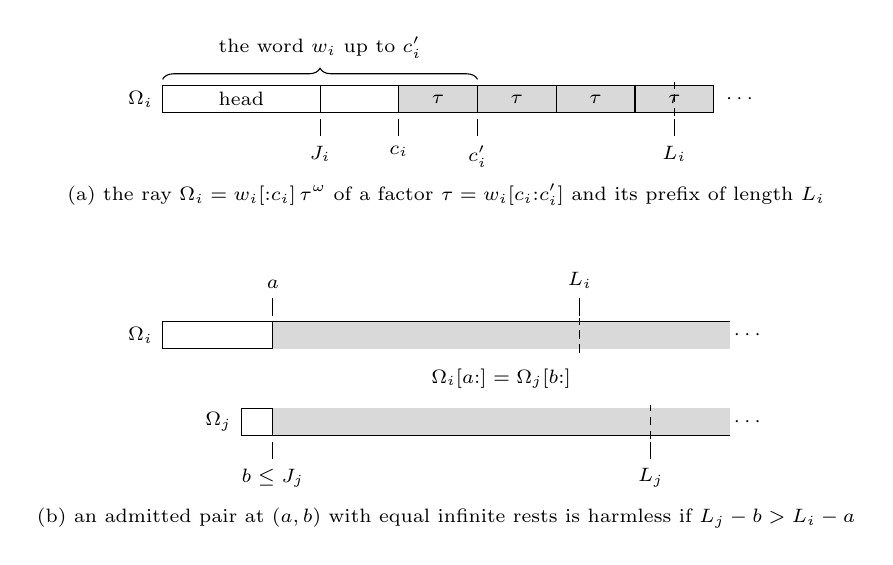
\begin{tikzpicture}[font=\scriptsize, >={Stealth[length=1.8mm]}]
\def\h{0.34}
%% (a) a ray
\begin{scope}
  \draw (0,0) rectangle (3.0,\h);
  \node at (1.0,0.5*\h) {head};
  \draw (2.0,0) -- (2.0,\h);
  \foreach \x in {3.0,4.0,5.0,6.0} {
    \draw[fill=black!15] (\x,0) rectangle (\x+1.0,\h);
    \node at (\x+0.5,0.5*\h) {$\tau$};
  }
  \node at (7.35,0.5*\h) {$\cdots$};
  \draw (2.0,-0.08) -- (2.0,-0.3) node[below] {$J_i$};
  \draw (3.0,-0.08) -- (3.0,-0.3) node[below] {$c_i$};
  \draw (4.0,-0.08) -- (4.0,-0.3) node[below] {$c_i'$};
  \draw[decorate, decoration={brace, amplitude=4pt}] (0,\h+0.08) -- (4.0,\h+0.08)
    node[midway, above=4pt] {the word $w_i$ up to $c_i'$};
  \draw (6.5,-0.08) -- (6.5,-0.3) node[below] {$L_i$};
  \draw[densely dashed] (6.5,-0.05) -- (6.5,\h+0.05);
  \node[left] at (0,0.5*\h) {$\Omega_i$};
  \node at (3.6,-1.05) {(a) the ray $\Omega_i=\wpre{w_i}{c_i}\,\tau^\omega$ of a factor
    $\tau=\wsub{w_i}{c_i}{c_i'}$ and its prefix of length $L_i$};
\end{scope}
%% (b) a constraint between two rays
\begin{scope}[yshift=-3.0cm]
  % host ray
  \draw (0,0) rectangle (7.2,\h);
  \fill[black!15] (1.4,0) rectangle (7.2,\h);
  \draw (1.4,0) -- (1.4,\h);
  \node[left] at (0,0.5*\h) {$\Omega_i$};
  \draw (1.4,\h+0.08) -- (1.4,\h+0.3) node[above] {$a$};
  \draw[densely dashed] (5.3,-0.05) -- (5.3,\h+0.05);
  \draw (5.3,\h+0.08) -- (5.3,\h+0.3) node[above] {$L_i$};
  % target ray
  \draw (1.0,-1.1) rectangle (7.2,-1.1+\h);
  \fill[black!15] (1.4,-1.1) rectangle (7.2,-1.1+\h);
  \draw (1.4,-1.1) -- (1.4,-1.1+\h);
  \node[left] at (1.0,-1.1+0.5*\h) {$\Omega_j$};
  \draw (1.4,-1.18) -- (1.4,-1.4) node[below] {$b\le J_j$};
  \draw[densely dashed] (6.2,-1.15) -- (6.2,-1.1+\h+0.05);
  \draw (6.2,-1.18) -- (6.2,-1.4) node[below] {$L_j$};
  \node at (4.3,-0.38) {$\wsuf{\Omega_i}{a}=\wsuf{\Omega_j}{b}$};
  \node at (7.45,0.5*\h) {$\cdots$};
  \node at (7.45,-1.1+0.5*\h) {$\cdots$};
  \node at (3.6,-2.15) {(b) an admitted pair at $(a,b)$ with equal infinite rests is harmless
    if $L_j-b>L_i-a$};
\end{scope}
\end{tikzpicture}
\caption{(a) A ray continues a word periodically after its first rejected
cut. (b) If the states at the cuts $a$ and $b$ are admitted and the rays
agree forever from these cuts, the prefixes of lengths $L_i$ and $L_j$ carry
this pair on the channel from $i$ to $j$ unless the rest of the target is
longer than the rest of the host. This gives the difference constraint
$L_j\ge L_i+(b-a+1)$.}
\label{fig:ray}
\end{figure}


So rays turn the unbounded problem of avoiding each other into a finite
graph condition. The remaining difficulty is to choose the rays so that
there is no positive cycle, and so that they create no comparisons with the
words that stay as they are.

\subsection{Closed Factors}\label{sec:tails-closed}

Let $x$ be the word of an eligible coordinate, with the first rejected cut
$J$, and let $t_1,\dots,t_m$ be words, the \emph{target words}: they stand
for the words of the other coordinates, whose rests may be compared with
rests of $x$. We want cuts $J\le c<c'$ of $x$ such that replacing the tail
of $x$ after $c$ by repetitions of $\tau=\wsub xc{c'}$ creates no comparison
in which this coordinate is the host and the target is one of the target
words. A comparison ends where the target word ends, so what matters at a
cut $e$ of the host is which rests of target words end there, and with which
state before them. For rests of bounded length this is finite information.

\begin{definition}[Suffix nodes and closed factors]\label{def:node}
Let $B\ge0$ be a \emph{window}. For a target word $t$, $v_B(t)$ denotes its
suffix of length $B$ if $\len t\ge B$; if $\len t<B$, there is no such word,
and we say that $v_B(t)$ has no occurrences. The \emph{suffix dictionary}
$\Dict_B$ consists of the empty word and the factors of the words $v_B(t_j)$,
or of $t_j$ itself if $\len{t_j}<B$. The \emph{suffix node} of a cut $e$ of
$x$ is the pair
\[
  \node_B(e)=\bigl(\sigma,\;q(e-\len\sigma)\bigr),
  \qquad\sigma\text{ the longest suffix of }\wpre xe\text{ in }\Dict_B,
\]
where $q(\cdot)$ is the state of the run of $x$. A factor $\wsub xc{c'}$
with $c<c'$ is \emph{closed at $B$} if $\node_B(c)=\node_B(c')$, and it is
\emph{free at $B$} if no occurrence of a word $v_B(t_j)$ ends at a cut of
$(c,c']$.
\end{definition}

\begin{example}\label{ex:nodes}
Let $t=0110$ be the only target word and $B=2$. Then $v_2(t)=10$ and
$\Dict_2=\{\eps,1,0,10\}$. In the host word $x=101100$, the longest suffix
of $\wpre x2=10$ in the dictionary is $10$, so $\node_2(2)=(10,q(0))$; at
the cut $3$ it is $1$, and $\node_2(3)=(1,q(2))$; at the cut $5$ it is again
$10$, and $\node_2(5)=(10,q(3))$. The factor $\wsub x25=110$ is closed at
$2$ if $q(0)=q(3)$. It is not free at $2$, because an occurrence of
$v_2(t)=10$ ends at the cut $5$.
\end{example}

The dictionary has at most $mB(B+1)/2+1$ words, whatever the alphabet, so
there are at most $N(mB(B+1)/2+1)$ suffix nodes. Since the dictionary is
closed under factors, the suffix node after one more letter is a function
of the suffix node before and of the letter, as in the automaton of Aho and
Corasick \cite{AhoCorasick75}. Hence along a repetition of a closed factor
the suffix nodes repeat (\cref{fig:closed-factor}).

\begin{lemma}[Pumping a closed factor]\label{lem:pump}
Let $\wsub xc{c'}$ be closed and free at $B$, with $c\ge J$, and let
$x'=\wpre xc\,\wpre{(\tau^\omega)}L$ with $\tau=\wsub xc{c'}$ and $L\ge
c'-c$. Then $x'$ is eligible with the first rejected cut $J$ and an immortal
endpoint, and for every target word $t_j$ and all cuts $b$ of $t_j$ and $a$ of
$x'$: if $\wsuf{t_j}b$ is a prefix of $\wsuf{x'}a$, then it is a prefix of
$\wsuf x{a^\circ}$ for a cut $a^\circ$ of $x$ that carries the same state as
the cut $a$ of $x'$.
\end{lemma}

%% closed-factor -- suffix nodes, a closed factor free of target occurrences.
\begin{figure}[t]
\centering
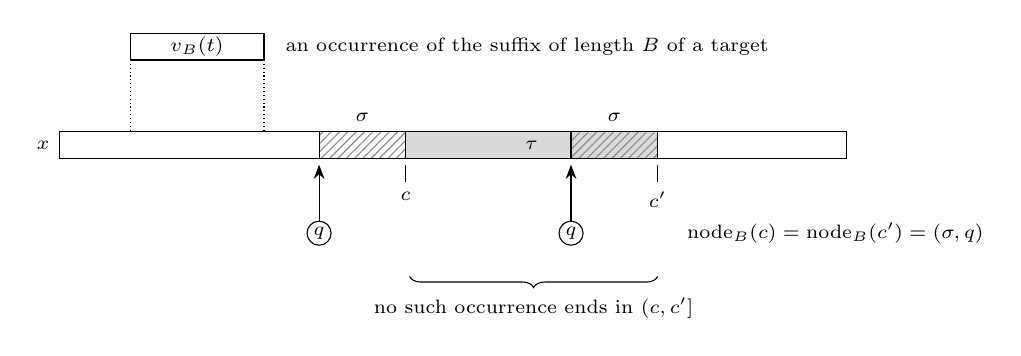
\begin{tikzpicture}[font=\scriptsize, >={Stealth[length=1.8mm]}]
\def\h{0.34}
% host word
\draw (0,0) rectangle (10.0,\h);
\node[left] at (0,0.5*\h) {$x$};
\draw[fill=black!15] (4.4,0) rectangle (7.6,\h);
\node at (6.0,0.5*\h) {$\tau$};
% suffix in dictionary at c and at c'
\draw[pattern=north east lines, pattern color=black!45] (3.3,0) rectangle (4.4,\h);
\draw[pattern=north east lines, pattern color=black!45] (6.5,0) rectangle (7.6,\h);
\node[above] at (3.85,\h) {$\sigma$};
\node[above] at (7.05,\h) {$\sigma$};
\draw (4.4,-0.08) -- (4.4,-0.3) node[below] {$c$};
\draw (7.6,-0.08) -- (7.6,-0.3) node[below] {$c'$};
\node[circle, draw, inner sep=1pt] (q1) at (3.3,-0.95) {$q$};
\node[circle, draw, inner sep=1pt] (q2) at (6.5,-0.95) {$q$};
\draw[->] (q1) -- (3.3,-0.08);
\draw[->] (q2) -- (6.5,-0.08);
\node[anchor=west] at (7.85,-0.95) {$\node_B(c)=\node_B(c')=(\sigma,q)$};
% a target suffix ending at an old cut
\draw (0.9,1.25) rectangle (2.6,1.25+\h);
\node at (1.75,1.25+0.5*\h) {$v_B(t)$};
\draw[densely dotted] (0.9,1.25) -- (0.9,\h);
\draw[densely dotted] (2.6,1.25) -- (2.6,\h);
\node[anchor=west] at (2.75,1.25+0.5*\h) {an occurrence of the suffix of length $B$ of a target};
\draw[decorate, decoration={brace, mirror, amplitude=4pt}] (4.45,-1.5) -- (7.6,-1.5)
  node[midway, below=4pt] {no such occurrence ends in $(c,c']$};
\end{tikzpicture}
\caption{A closed factor. The cuts $c<c'$ of the host word $x$ have the same
suffix node: the same longest suffix $\sigma$ in the suffix dictionary of the
targets at the window $B$, and the same state $q$ before it. If moreover no
occurrence of the suffix of length $B$ of a target ends in $(c,c']$, the
factor $\tau=\wsub xc{c'}$ can be repeated any number of times without
creating a comparison with a target (\cref{lem:pump}).}
\label{fig:closed-factor}
\end{figure}


A rest of a target word of length at most $B$ that ends at a cut of $x'$ lies in
the dictionary, so it is a suffix of the word of the suffix node, and it ends
at a cut of $x$ with the same node. A longer rest ends with $v_B(t_j)$, which
by freedom ends only at cuts up to $c$, where $x'$ and $x$ coincide.

Closed factors exist by the pigeonhole principle; the point is to find one
that is free. The occurrences of $v_B(t)$ can be avoided if they are
sparse, and they are sparse unless $t$ has a periodic suffix at the scale
of $B$. This is measured by \emph{suffix chains}: for a window $b$ with
$1\le b\le\len t$ let $\gap_t(b)$ be the distance from the end of $t$ to the
end of the previous occurrence of $v_b(t)$ in $t$, if there is one; a chain
is a sequence $b_0<b_1<\cdots$ of windows with $b_{r+1}=b_r+\gap_t(b_r)$,
and its number of \emph{steps} is the number of its members after the first.
Along a chain the suffixes $v_{b_r}(t)$ are prefixes of one another.

\begin{example}\label{ex:chain}
Let $t=ababab$. The suffix $v_1(t)=b$ also ends two letters before the end
of $t$, so $\gap_t(1)=2$ and the chain from the window $1$ continues with
$3$. The suffix $v_3(t)=bab$ again ends two letters before the end, so
$\gap_t(3)=2$, and the next window is $5$. The suffix $v_5(t)=babab$ has no
other occurrence, and the chain $1<3<5$ stops after two steps
(\cref{fig:chain}). A periodic suffix thus gives a chain whose gap is the
period, with about as many steps as the suffix has periods. In contrast,
for $t=aabbab$ the chain from the window $1$ is $1<3$: the gap of $b$ is
again $2$, but $bab$ occurs only once. A chain stops at a window whose
suffix occurs only at the end of $t$, and a long chain with small gaps
indicates a long periodic suffix.
\end{example}

%% chain -- the suffix chain of ababab from the window 1.
\begin{figure}[t]
\centering
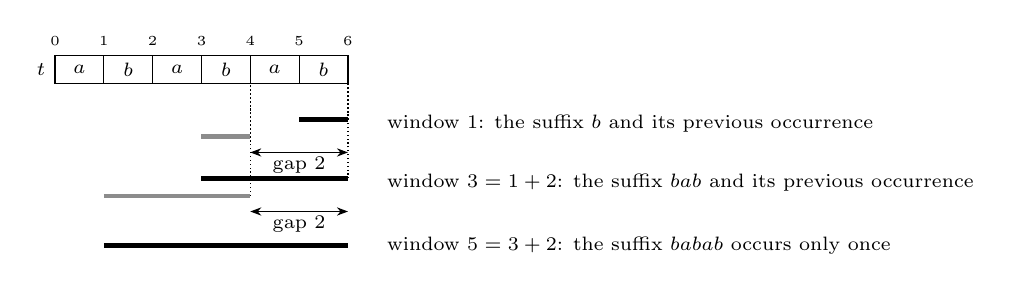
\begin{tikzpicture}[font=\scriptsize, x=0.62cm, y=1cm]
\def\h{0.36}
\foreach \c [count=\i from 0] in {a,b,a,b,a,b} {
  \draw (\i,0) rectangle (\i+1,\h);
  \node at (\i+0.5,0.5*\h) {$\c$};
}
\node[left] at (0,0.5*\h) {$t$};
\foreach \i in {0,...,6} { \node[above, font=\tiny] at (\i,\h) {$\i$}; }
%% rows: window b, suffix [6-b,6], previous occurrence [6-b-2,6-2]
\foreach \b/\y in {1/-0.45,3/-1.2} {
  \pgfmathsetmacro{\l}{6-\b}
  \draw[line width=1.6pt] (\l,\y) -- (6,\y);
  \draw[line width=1.6pt, black!45] (\l-2,\y-0.22) -- (4,\y-0.22);
  \draw[densely dotted] (6,\y) -- (6,0);
  \draw[densely dotted] (4,\y-0.22) -- (4,0);
  \draw[<->, >={Stealth[length=1.4mm]}] (4,\y-0.42) -- node[below, inner sep=1.5pt] {gap $2$} (6,\y-0.42);
}
\draw[line width=1.6pt] (1,-2.05) -- (6,-2.05);
\node[anchor=west] at (6.6,-0.5) {window $1$: the suffix $b$ and its previous occurrence};
\node[anchor=west] at (6.6,-1.25) {window $3=1+2$: the suffix $bab$ and its previous occurrence};
\node[anchor=west] at (6.6,-2.05) {window $5=3+2$: the suffix $babab$ occurs only once};
\end{tikzpicture}
\caption{The suffix chain $1<3<5$ of $t=ababab$ (\cref{ex:chain}). At each
window the suffix (black) is compared with its previous occurrence (gray);
the distance between their ends is the gap, which is added to the window.
The suffixes $b$, $bab$, $babab$ are prefixes of one another.}
\label{fig:chain}
\end{figure}


\begin{lemma}[Closed factors free of the target words]\label{lem:closed-free}
For every number $s$ there are computable functions $\Lb_m$ and $\Wb_m$,
which depend on $s$ and are nondecreasing in the window, with the following
property. Let $1\le b_0\le b$, and suppose that every suffix chain of every
target word that starts at a window of at least $b_0$ has at most $s$
steps. Then every sequence of $\Lb_m(b)$
consecutive cuts of $x$ contains cuts $c<c'$ and there is a window $B$ with
$b\le B\le\Wb_m(b)$ such that $\wsub xc{c'}$ is closed and free at $B$ and
$B<c'-c\le\Fb(B)$, where $\Fb(B)=(B+1)\,N\,(mB(B+1)/2+1)$.
\end{lemma}

The proof treats the target words one after the other. For one target word
it follows a suffix chain as long as the gaps stay below the length needed
for the remaining ones; the chain stops within $s$ steps, at a window where the
occurrences of the suffix are far apart. Either a long stretch of the given
cuts is free at this window, or the occurrences come so regularly that a
slightly larger window has no occurrence at all after the first one. The
base case is a pigeonhole on the suffix nodes of cuts that are $B+1$ apart,
which makes the closed factor longer than its window. The functions $\Lb_m$
are polynomials in the window whose degree depends on $s$ and $m$; this
matters for the complexity bound (\cref{sec:complexity}).

\subsection{Scales of Periodicity}\label{sec:tails-levels}

%% types -- the three types of coordinates at a stable scale.
\begin{figure}[t]
\centering
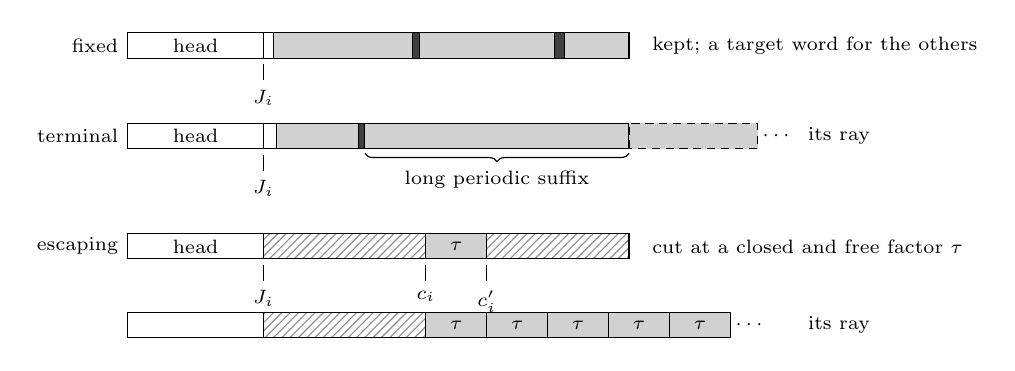
\begin{tikzpicture}[font=\scriptsize, >={Stealth[length=1.8mm]}, xscale=0.86]
\def\h{0.32}
\tikzset{pf/.style={fill=black!18}, ex/.style={fill=black!75}}
%% fixed
\begin{scope}
  \draw (0,0) rectangle (7.4,\h);
  \node at (1.0,0.5*\h) {head};
  \draw (2.0,-0.08) -- (2.0,-0.28) node[below] {$J_i$};
  \draw (2.0,0) -- (2.0,\h);
  \draw[pf] (2.15,0) rectangle (4.2,\h);
  \draw[ex] (4.2,0) rectangle (4.3,\h);
  \draw[pf] (4.3,0) rectangle (6.3,\h);
  \draw[ex] (6.3,0) rectangle (6.45,\h);
  \draw[pf] (6.45,0) rectangle (7.4,\h);
  \node[left] at (0,0.5*\h) {fixed};
  \node[anchor=west] at (7.6,0.5*\h) {kept; a target word for the others};
\end{scope}
%% terminal
\begin{scope}[yshift=-1.15cm]
  \draw (0,0) rectangle (7.4,\h);
  \node at (1.0,0.5*\h) {head};
  \draw (2.0,-0.08) -- (2.0,-0.28) node[below] {$J_i$};
  \draw (2.0,0) -- (2.0,\h);
  \draw[pf] (2.2,0) rectangle (3.4,\h);
  \draw[ex] (3.4,0) rectangle (3.5,\h);
  \draw[pf] (3.5,0) rectangle (7.4,\h);
  \draw[pf, densely dashed] (7.4,0) rectangle (9.3,\h);
  \node at (9.6,0.5*\h) {$\cdots$};
  \draw[decorate, decoration={brace, mirror, amplitude=3pt}] (3.5,-0.06) -- (7.4,-0.06)
    node[midway, below=3pt] {long periodic suffix};
  \node[left] at (0,0.5*\h) {terminal};
  \node[anchor=west] at (9.9,0.5*\h) {its ray};
\end{scope}
%% escaping
\begin{scope}[yshift=-2.55cm]
  \draw (0,0) rectangle (7.4,\h);
  \node at (1.0,0.5*\h) {head};
  \draw (2.0,-0.08) -- (2.0,-0.28) node[below] {$J_i$};
  \draw (2.0,0) -- (2.0,\h);
  \draw[pattern=north east lines, pattern color=black!45] (2.0,0) rectangle (7.4,\h);
  \draw[pf] (4.4,0) rectangle (5.3,\h);
  \node at (4.85,0.5*\h) {$\tau$};
  \draw (4.4,-0.08) -- (4.4,-0.28) node[below] {$c_i$};
  \draw (5.3,-0.08) -- (5.3,-0.28) node[below] {$c_i'$};
  \node[left] at (0,0.5*\h) {escaping};
  %% the ray
  \draw (0,-1.0) rectangle (4.4,-1.0+\h);
  \draw[pattern=north east lines, pattern color=black!45] (2.0,-1.0) rectangle (4.4,-1.0+\h);
  \draw (2.0,-1.0) -- (2.0,-1.0+\h);
  \foreach \x in {4.4,5.3,6.2,7.1,8.0} {
    \draw[pf] (\x,-1.0) rectangle (\x+0.9,-1.0+\h);
    \node at (\x+0.45,-1.0+0.5*\h) {$\tau$};
  }
  \node at (9.2,-1.0+0.5*\h) {$\cdots$};
  \node[anchor=west] at (9.9,-1.0+0.5*\h) {its ray};
  \node[anchor=west] at (7.6,0.5*\h) {cut at a closed and free factor $\tau$};
\end{scope}
\end{tikzpicture}
\caption{The three types of coordinates at a stable scale. Periodic factors
with short periods are gray, exceptional positions black, and text without
such a structure is hatched. A fixed coordinate with an immortal endpoint
has a tail of few periodic factors and no long periodic suffix; its word is
kept. A terminal coordinate ends with a long periodic suffix and is
continued by the ray of this suffix. An escaping coordinate is far from
periodic at this scale; its tail is cut at one of many closed and free
factors $\tau$ and continued by $\tau^\omega$.}
\label{fig:types}
\end{figure}


Which coordinates should be replaced by rays, and at which scale? A tail
that already consists of few periodic stretches should be kept: its word is
a harmless target word, with short suffix chains. A tail that is far from
periodic offers many closed factors with different onsets to choose from.
The two cases must be separated by a gap in scale, because the closed
factors of one word have to avoid the suffixes of the others. We therefore
measure periodicity at a sequence of \emph{scales} $l=0,1,2,\dots$, each
much coarser than the one before. Scale $l$ comes with four numbers, defined
by a recursion on $l$ in \cref{app:tails-levels} and nondecreasing in $l$:
\begin{itemize}
\item $e_l$ bounds the periods that count as short at scale $l$;
\item $T_l$ bounds the number of positions of a tail that may lie outside
  its periodic factors;
\item $Y_l$ is the length from which a periodic suffix counts as long;
\item $b_l$ is the \emph{initial window} of scale $l$, the smallest window
  at which closed factors are searched.
\end{itemize}
The recursion makes each scale dominate the previous ones: for instance
$b_{l+1}>(N+1)\,e_l$, and $Y_{l+1}$ exceeds every length that can be
assembled from $T_l$ exceptional positions and boundedly many periods
$e_{l+1}$ (inequalities (L1)--(L5) of \cref{app:tails-levels}). The number
of periodic factors that we allow is governed by the constant
\[
  \Qc=4+2(k-1)(N-1).
\]
Its value is chosen for the count in \cref{sec:tails-choice}: a coordinate that
is not almost periodic offers at least $\Qc-1$ suitable rays, and each of
the other $k-1$ coordinates can spoil at most $2(N-1)$ of them, so one
remains because $\Qc-1>2(k-1)(N-1)$.

\begin{definition}[Almost periodic tails]\label{def:cover}
An eligible coordinate $i$ has property $F_l$ if all positions of its
rejected tail, except at most $T_l$, lie in at most $\Qc+1$ factors of $w_i$
with periods at most $e_l$. It has property $K_l$ if it has $F_l$ and the
longest suffix of $w_i$ with a period of at most $e_l$ is shorter than
$Y_l$.
\end{definition}

So $F_l$ says that the tail consists of few periodic stretches, up to few
exceptional positions, and $K_l$ says in addition that the word does not
end with a long periodic stretch. For instance, for three different
letters $a,b,c$, a tail $(ab)^{r}c\,(ba)^{r'}$ has $F_l$ for every $l$, with
two factors of period $2$ and one exceptional position, whatever $r$ and
$r'$ are, and it has $K_l$ exactly when $2r'<Y_l$. In contrast, a tail
fails $F_l$ when its periodic stretches with periods up to $e_l$ are so
many and so short that any $\Qc+1$ of them leave more than $T_l$ positions
uncovered.

Both properties are inherited from a scale to the next
(\cref{lem:levels-mono}); for $K_l$ this uses the periodicity lemma of Fine
and Wilf \cite{FineWilf65}. There are $2k$ properties $F_l,K_l$ of the $k$
coordinates, each of which changes at most once as $l$ grows, so among the
scales up to $3(2k+1)$ there is a \emph{stable} scale $l\ge2$: no coordinate
changes its status with respect to $F$ between $l-1$ and $l$, or with
respect to $K$ between $l-2$ and $l-1$. At a stable scale every coordinate
is of exactly one of three types (\cref{fig:types}).
\begin{itemize}
\item \emph{Fixed}: the endpoint is mortal, or the coordinate has $K_{l-2}$.
  Its word is kept. Its suffix chains from the initial window $b_l$ of
  scale $l$ on have at most $\Qc+N$ steps (\cref{lem:chains}); for a mortal
  endpoint this follows from \cref{lem:distinct}.
\item \emph{Terminal}: the endpoint is immortal and the coordinate has
  $F_{l-1}$ but not $K_{l-1}$. Its word ends with a long suffix of period at
  most $e_{l-1}$, and it is continued by the ray of this suffix. The ray
  contains the whole word $w_i$.
\item \emph{Escaping}: the endpoint is immortal and the coordinate does not
  have $F_l$. Its tail is cut at a suitable closed factor and continued
  periodically.
\end{itemize}
The number of steps of a suffix chain of a fixed word does not grow with the
scale; this is what keeps the recursion of the numbers $e_l,T_l,Y_l,b_l$,
and with it the final bound, elementary.

\subsection{Choosing Compatible Rays}\label{sec:tails-choice}

We fix a stable scale $l$. The target words are the words of the fixed
coordinates. For a terminal
coordinate, the last $pN!$ letters of its periodic suffix, $p$ the period,
form a factor that is closed and free at a suitable window
(\cref{lem:terminal}). For an escaping coordinate $v$, \cref{lem:closed-free}
provides a closed and free factor in every stretch of $\Lb_k(b_l)$ cuts of
the tail, a \emph{candidate}. If the rays of the candidates had at most $\Qc+1$ different
onsets, the periodic stretches from these onsets would cover the tail up to
$T_l$ positions, and $v$ would have $F_l$. So there are candidates whose
rays have at least $\Qc+2$ different onsets, of which at most three lie at
or before $J_v$ (\cref{lem:candidates}); this leaves $\Qc-1$ candidate rays
with different onsets after $J_v$.

It remains to exclude positive cycles in the ray system. A constraint $i\to
j$ requires the rays to agree forever from cuts $a$ and $b\le J_j$. If the
onset of $\Omega_j$ lies after $J_j$, \cref{lem:ray-compare} aligns the
onsets, and the stretch $X_j=\wsub{\Omega_j}{J_j}{\onset(\Omega_j)}$ of the
target between its first rejected cut and its onset is copied into the host
just before the onset of the host. Following a cycle backwards from an
escaping coordinate $v$, these stretches grow strictly, so the cycle cannot
return to $v$, unless one of three \emph{forbidden overlaps} of $v$ with
the ray of another coordinate $u$ occurs (\cref{def:overlaps}). In the
first, $X_v$ is a suffix of the text of the ray of $u$ before its onset,
the onset of $u$ lies after $J_u$, and $X_u$ is not longer than $X_v$. In
the second, $X_v$ is such a suffix, the onset of $u$ lies at or before
$J_u$, and the two rays have the same periodic part. In the third, the
roles are exchanged: $X_u$ is a nonempty suffix of the text of the ray of
$v$ before its onset, and $X_v$ is not longer than $X_u$.

\begin{lemma}[Compatible candidates]\label{lem:compatible}
\begin{enumerate}
\item\label{it:compat-count} For a terminal ray or an escaping ray chosen
  earlier, of a coordinate $u\ne v$, at most $2(N-1)$ candidates of $v$ with
  pairwise different onsets after $J_v$ have a forbidden overlap with it.
\item\label{it:compat-cycle} A ray with its onset after its first rejected
  cut that has no forbidden overlap with any other ray lies on no cycle of
  the ray system.
\end{enumerate}
\end{lemma}

The count in \eqref{it:compat-count} is again an application of
\cref{lem:distinct}: different candidates with the same kind of overlap give
cuts at or before a first rejected cut that carry different states. Since
$\Qc-1>2(k-1)(N-1)$, the escaping coordinates can be treated one after the
other, each taking one of its $\Qc-1$ candidates that has no forbidden
overlap with the at most $k-1$ rays chosen before. Cycles then pass through terminal rays only, and for these the
lengths of the original words satisfy all constraints, because $W$ is a hole.
So there is no positive cycle. Solving the ray system above sufficiently
large lower bounds and applying \cref{lem:pump,lem:ray-prefixes} gives:

\begin{proposition}[Holes with periodic tails]\label{prop:run-cover}
There are computable numbers $D$ and $E_0$, depending on $k$ and $N$, such
that every structural reader with a hole has a hole in which the rejected
tail of every coordinate with an immortal endpoint is covered, up to $E_0$
positions in total, by at most $\Qc+3$ maximal periodic factors with periods
at most $D$ and lengths at least $2D$.
\end{proposition}

\subsection{Compressing the Pieces}\label{sec:tails-compression}

A \emph{piece} of period $d$ in a tuple is a maximal factor of one word that
has period $d$, length at least $2d$ and a primitive \emph{root}, its first
$d$ letters; a word is primitive if it is not a power of a shorter word.
Pieces are the runs, or maximal repetitions, of combinatorics on words
\cite{KolpakovKucherov99}; we say piece because run already means the run of
an automaton. The maximal periodic factors of \cref{prop:run-cover} are
pieces. The pieces whose roots are conjugates (rotations) of a primitive
word $\zeta$ form the \emph{class} of $\zeta$. The \emph{follower} of a
piece is the rest of its word after it. For example, the word $abababb$ has
the piece $ababab$ of period $2$, with the root $ab$ and the follower $b$,
and the piece $bb$ of period $1$, with the root $b$ and the empty follower;
in $bababa$ the whole word is a piece of the class of $ab$, with the root
$ba$.

%% compression -- an admissible deletion on two pieces of a class with comparable followers.
\begin{figure}[!b]
\centering
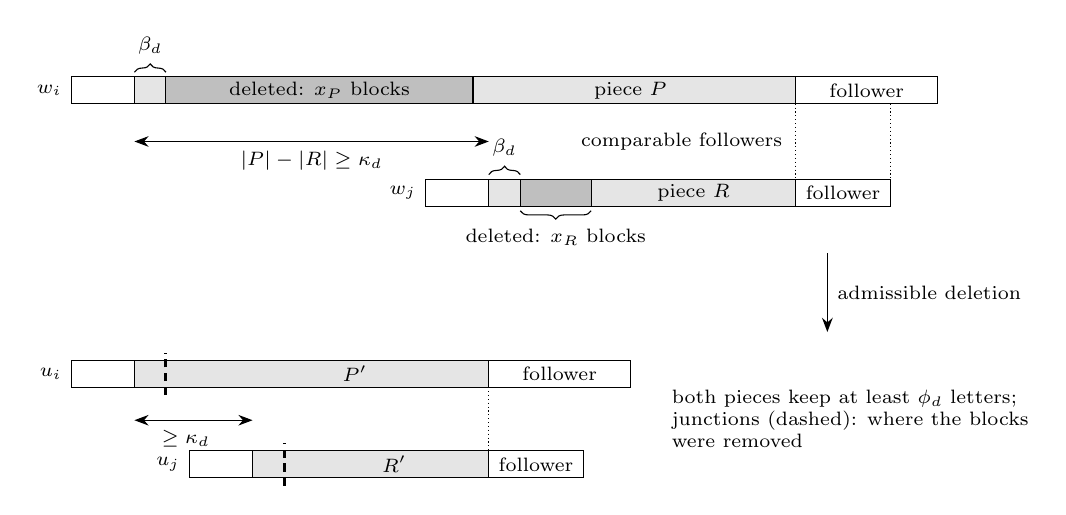
\begin{tikzpicture}[font=\scriptsize, >={Stealth[length=1.8mm]}]
\def\h{0.34}
%% before
\begin{scope}
  % word i with a long piece P = [0.8,9.2], site [1.2,5.1]
  \draw (0,0) rectangle (11.0,\h);
  \node[left] at (0,0.5*\h) {$w_i$};
  \draw[fill=black!10] (0.8,0) rectangle (9.2,\h);
  \draw[fill=black!25] (1.2,0) rectangle (5.1,\h);
  \node at (3.15,0.5*\h) {deleted: $x_P$ blocks};
  \node at (7.1,0.5*\h) {piece $P$};
  \node at (10.1,0.5*\h) {follower};
  \draw[decorate, decoration={brace, amplitude=3pt}] (0.8,\h+0.06) -- (1.2,\h+0.06)
    node[midway, above=3pt] {$\beta_d$};
  % word j with a piece R = [5.3,9.2], site [5.7,6.6], comparable follower
  \draw (4.5,-1.3) rectangle (10.4,-1.3+\h);
  \node[left] at (4.5,-1.3+0.5*\h) {$w_j$};
  \draw[fill=black!10] (5.3,-1.3) rectangle (9.2,-1.3+\h);
  \draw[fill=black!25] (5.7,-1.3) rectangle (6.6,-1.3+\h);
  \node at (7.9,-1.3+0.5*\h) {piece $R$};
  \node at (9.8,-1.3+0.5*\h) {follower};
  \draw[decorate, decoration={brace, amplitude=3pt}] (5.3,-1.3+\h+0.06) -- (5.7,-1.3+\h+0.06)
    node[midway, above=3pt] {$\beta_d$};
  \draw[decorate, decoration={brace, mirror, amplitude=3pt}] (5.7,-1.36) -- (6.6,-1.36)
    node[midway, below=3pt] {deleted: $x_R$ blocks};
  \draw[densely dotted] (9.2,0) -- (9.2,-1.3+\h);
  \draw[densely dotted] (10.4,0) -- (10.4,-1.3+\h);
  \node[anchor=east] at (9.15,-0.48) {comparable followers};
  \draw[<->] (0.8,-0.48) -- node[below] {$\len P-\len R\ge\kappa_d$} (5.3,-0.48);
\end{scope}
%% after
\begin{scope}[yshift=-3.6cm]
  % P' = [0.8,5.3], junction at 1.2
  \draw (0,0) rectangle (7.1,\h);
  \node[left] at (0,0.5*\h) {$u_i$};
  \draw[fill=black!10] (0.8,0) rectangle (5.3,\h);
  \draw[line width=1.1pt, densely dashed] (1.2,-0.1) -- (1.2,\h+0.1);
  \node at (3.6,0.5*\h) {$P'$};
  \node at (6.2,0.5*\h) {follower};
  % R' = [2.3,5.3], junction at 2.7
  \draw (1.5,-1.15) rectangle (6.5,-1.15+\h);
  \node[left] at (1.5,-1.15+0.5*\h) {$u_j$};
  \draw[fill=black!10] (2.3,-1.15) rectangle (5.3,-1.15+\h);
  \draw[line width=1.1pt, densely dashed] (2.7,-1.25) -- (2.7,-1.15+\h+0.1);
  \node at (4.1,-1.15+0.5*\h) {$R'$};
  \node at (5.9,-1.15+0.5*\h) {follower};
  \draw[densely dotted] (5.3,0) -- (5.3,-1.15+\h);
  \draw[<->] (0.8,-0.42) -- node[below, xshift=-1mm] {$\ge\kappa_d$} (2.3,-0.42);
  \node[anchor=west, align=left] at (7.5,-0.4) {both pieces keep at least $\phi_d$ letters;\\
    junctions (dashed): where the blocks\\ were removed};
\end{scope}
\draw[->, semithick] (9.6,-1.9) -- (9.6,-2.9) node[midway, right] {admissible deletion};
\end{tikzpicture}
\caption{An admissible deletion (schematic). Two pieces $P$ and $R$ of the
same class whose followers are comparable can be aligned by a comparison, so
they must be shortened consistently. Each loses a number of blocks of $m_d$
letters (darker), starting $\beta_d$ letters after its start, where the states
of the run have become periodic with period $m_d$. Here $P$ is longer than
$R$ by at least the threshold $\kappa_d$; it loses more blocks, but remains longer
by at least $\kappa_d$. Pieces whose lengths differ by less than $\kappa_d$
lose the same number of blocks.}
\label{fig:compression}
\end{figure}


Inside a piece of period $d$ the states of the run are periodic with period
$m_d=d\cdot N!$ after $\alpha_d=Nd$ letters. So a block of $m_d$ letters
can be deleted from the interior of a piece without changing the later
states. Deleting blocks from one piece only would be visible to
comparisons that align this piece with a piece of the same class in another
word, or in the same word. Two pieces can be aligned by a comparison that
continues beyond them only if their followers are comparable, which leads to
the following conditions (\cref{fig:compression}). They use three lengths:
\[
  \beta_d=\alpha_d+m_d,\qquad\kappa_d=2\beta_d+m_d,\qquad
  \phi_d=6\beta_d+2m_d.
\]
The deleted blocks begin $\beta_d$ letters after the start of a piece: this
skips the transient $\alpha_d$ of the states and one more block. The number
$\kappa_d$ is the threshold for the difference of the lengths of two pieces
with comparable followers. Pieces that differ by less are shortened alike.
A difference of at least $\kappa_d$ is kept, and it ensures that where the
shorter piece begins, the states of the longer one are already periodic, so
that it does not matter how many blocks each of them has lost. Finally,
$\phi_d$ is the length that a shortened piece keeps; it leaves room for the
$\beta_d$ letters before the deleted blocks and for $5\beta_d+2m_d$ letters
after them, so that both ends of the piece and the letters next to them are
not affected. For instance, for $N=3$ and $d=2$ we get $\alpha_d=6$,
$m_d=12$, $\beta_d=18$, $\kappa_d=48$ and $\phi_d=132$.

\begin{definition}[Admissible deletion]\label{def:admissible}
An \emph{admissible deletion} of the class of $\zeta$, with $d=\len\zeta$,
deletes $x_P$ blocks of $m_d$ letters from every piece $P$ of the class,
starting $\beta_d$ letters after the start of $P$, such that
\begin{itemize}
\item a piece that is shortened keeps at least $\phi_d$ letters;
\item two pieces with comparable followers whose lengths differ by less
  than $\kappa_d$ lose the same number of blocks;
\item if $P$ and $R$ have comparable followers and $R$ is longer than $P$
  by at least $\kappa_d$, it remains longer by at least $\kappa_d$.
\end{itemize}
\end{definition}

\begin{lemma}[Admissible deletions]\label{lem:admissible}
The result of an admissible deletion dominates the original tuple. If the
tuple is a hole, the result is a hole with the same endpoints, its first
rejected cuts are the images of the original ones, and pieces of other
classes with periods at most $d$ and lengths at least $2d$ are not affected.
\end{lemma}

The numbers $x_P$ are the solution of another system of difference
constraints, and the least solution is small unless long chains of
constraints force a piece to stay long. Such a chain is a path in the graph
that joins pieces with comparable followers. Comparability of followers is
comparability in the forest of the prefix order, and a simple path in the
comparability graph of a forest of height $h$ has at most $2^h-1$ vertices.
For the pieces that end at or before the first rejected cut of their word,
or lie in words with mortal endpoints, comparable followers begin at cuts
with different states (\cref{lem:distinct}), so their height is at most
$k(N-1)$. The other pieces end in the rejected tails of immortal
coordinates, and their number is bounded by \cref{prop:run-cover}.
Splitting a path at these pieces gives a bound that is \emph{linear} in
their number.

\begin{lemma}[The cap]\label{lem:cap}
Suppose that every set of pieces of the class that have pairwise comparable
followers and are not among $r$ exceptional pieces has at most $h$ elements.
Then there is an admissible deletion after which every piece of the class
has length at most
\[
  \phi_d+m_d+\bigl((r+1)\,2^{h}-1\bigr)(\kappa_d+m_d).
\]
\end{lemma}

Starting from the hole of \cref{prop:run-cover}, we call the at most
$k(\Qc+3)$ pieces that cover its immortal tails the \emph{designated}
pieces. We compress the class of a designated piece of the largest period,
count the positions of the shortened designated pieces of this class among
the uncovered positions, and repeat with the remaining designated pieces.
After at most $k(\Qc+3)$ passes all immortal tails are short.

\begin{theorem}[Rejected tails, with the bound]\label{thm:tails-bound}
For $k\ge1$ and $N\ge1$, let $E_0$ and $D$ be as in \cref{prop:run-cover},
let $g=k(\Qc+3)$, and define
\[
  E_{r+1}=E_r+(g-r)\,\Bigl(\phi_D+m_D+\bigl((2(g-r)+E_r+1)\,2^{k(N-1)}-1\bigr)
  (\kappa_D+m_D)\Bigr).
\]
Then \cref{thm:tails} holds with
$\TailB(k,N)=E_g\le\expo_2\bigl((k+N+20)^{2k+5}\bigr)$ for $k\ge1$ and
$N\ge1$, and with $\TailB(0,N)=0$.
\end{theorem}

The closed form is proved in \cref{app:complexity-closed}.

\section{The Decision Procedures}
\label{sec:decision}

We now assemble the decision procedures for disjunctive entailment: over
arbitrary trees, where the previous sections apply directly; over regular
trees, where the answers are the same; over finite trees, where they differ
only through satisfiability; and for the signature $\BF$, which reduces to
$\BFT$. \Cref{thm:main} then follows with \cref{prop:sentences}. Proofs
omitted here are in \cref{app:classes}.

\subsection{Arbitrary Trees}\label{sec:decision-arbitrary}

\begin{theorem}[Arbitrary trees]\label{thm:decide-arbitrary}
Disjunctive entailment between flat constraints over $\BFT$ is decidable
over $\Trees$, uniformly in the number of queries, the arity and the
variance.
\end{theorem}

\begin{proof}
Let $\Gamma$ be a constraint and $(x_1,y_1),\dots,(x_k,y_k)$ queries.
\begin{enumerate}
\item Decide whether $\Gamma$ is satisfiable over $\Trees$
  (\cref{lem:sat-decidable}). If it is not, the entailment holds.
\item Otherwise, for each of the $2^k$ mode vectors $\bar\mu$, compute the
  reader $M_{\bar\mu}$ of \cref{def:compile} and test all tuples of paths of
  total length at most $\Hole(k,N)$, where $N$ is the number of its states,
  for being holes. The entailment fails if and only if a hole is found.
  For $k=0$ there is one mode vector, the empty one, and $\Hole(0,N)=0$; the
  empty tuple is a hole, and the entailment fails, as it must for a
  satisfiable constraint.
\end{enumerate}
The second step is correct by \cref{thm:reduction,thm:small-hole}. Whether a tuple is a hole is checked directly from
\cref{def:hole}.
\end{proof}

\begin{lemma}[Satisfiability]\label{lem:sat-decidable}
It is decidable whether a flat constraint over $\BFT$ is satisfiable over
$\Trees$.
\end{lemma}

Satisfiability is in fact decidable in polynomial time
\cite{KozenPalsbergSchwartzbach94,PalsbergWandOKeefe97}. In our setting it
is the question whether the least closure is consistent and contains no
forbidden atom (\cref{sec:readers-atoms}), and for each signed variable the
paths of its atoms in the least closure form a regular language accepted by
the automaton of lower runs (\cref{app:reduction-lc}).

\subsection{Regular Trees}\label{sec:decision-regular}

\begin{theorem}[Regular trees]\label{thm:decide-regular}
For every flat constraint $\Gamma$ over $\BFT$ and all queries,
\[
  \Gamma\entails_{\TreesReg}x_1\le y_1\vee\dots\vee x_k\le y_k
  \iff
  \Gamma\entails_{\Trees}x_1\le y_1\vee\dots\vee x_k\le y_k .
\]
\end{theorem}

\begin{proof}[Proof sketch]
A regular countermodel is a countermodel, which gives the implication from
right to left. Conversely, let $\rho$ be a countermodel over $\Trees$, with
seeds $A_i$ and exclusions $B_i$ as in \cref{sec:readers-modes}. By
\cref{thm:realization} the hull of the seeds is a solution set that
contains the seeds and none of the exclusions, so the corresponding
assignment is a countermodel. For each signed variable $x^s$, the paths $w$
with $(x^s,w)$ in the hull form a regular language: those from the least
closure do, and by \cref{lem:cuts} those derived from the seed $(p_i,w_i)$
are the words $v\,\wsuf{w_i}a\,\sigma$, for a cut $a$ of $w_i$, a word $v$
with $\Dn(x^s,v)\cap\Up(p_i,\wpre{w_i}a)\ne\varnothing$ and an arbitrary
word $\sigma$. A tree whose two cones are regular languages has finitely
many subtrees, because the subtree at a position is determined by the
residuals of the two cones and the polarity of the position
(\cref{lem:regular-cones}).
\end{proof}

So the hull of the seeds, the least countermodel with the given witnesses,
is a regular tree in every component, and it is computable from a hole.

\subsection{Finite Trees}\label{sec:decision-finite}

Over finite trees a constraint can be unsatisfiable although it is
satisfiable over $\Trees$; for a unary constructor, $x\le f(x)$, $f(x)\le x$
is an example. This is
the only difference.

\begin{theorem}[Finite trees]\label{thm:decide-finite}
For every flat constraint $\Gamma$ over $\BFT$ and all queries,
$\Gamma\entails_{\TreesFin}x_1\le y_1\vee\dots\vee x_k\le y_k$ holds if and
only if $\Gamma$ is unsatisfiable over $\TreesFin$ or
$\Gamma\entails_{\Trees}x_1\le y_1\vee\dots\vee x_k\le y_k$. Satisfiability
over $\TreesFin$ is decidable, and hence so is disjunctive entailment over
$\TreesFin$.
\end{theorem}

The nontrivial direction is to turn a countermodel over $\Trees$ into a
finite one when $\Gamma$ has some finite solution. A countermodel is
described by finitely many \emph{observations}: the $k$ seeds belong to its
set of atoms and the $k$ exclusions do not. Each observation is equivalent
to a bound of a variable by a finite tree. For instance, for a covariant
constructor, $(x^{\sgp},w)\in S_\rho$ says that $\rho(x)$ lies above the
finite tree that has $f$ along the path $w$, $\Top$ at its end and $\Bot$
beside it, and $(x^{\sgp},w)\notin S_\rho$ says that $\rho(x)$ lies below the
finite tree that has $f$ along $w$ and at its end, and $\Top$ everywhere
else (\cref{lem:observations}). The theorem then follows from a pinning
property of finite solutions:

\begin{lemma}[Pinning]\label{lem:pinning}
Suppose that $\Gamma$ has a solution over $\TreesFin$ and that some solution
of $\Gamma$ over $\Trees$ satisfies finitely many bounds $g\le x$ and $x\le
g'$ of variables by finite trees. Then some solution of $\Gamma$ over
$\TreesFin$ satisfies these bounds.
\end{lemma}

Its proof (\cref{app:classes-finite}) first treats a covariant
constructor. It compiles the bounds into flat literals on fresh variables,
which only hang finite trees below or above existing variables, and shows
that they create no \emph{cycle clash}, the obstruction to finite
satisfiability of \cite{Zhao26}. With variance, it translates the
constraint into a covariant constraint on the signed variables and makes the
finite solution obtained there symmetric under the exchange of the two signs,
by a median of trees.

\subsection{The Signature \texorpdfstring{$\BF$}{\{bot, f\}}}\label{sec:decision-bf}

Let $f$ be covariant. The trees over $\BF$ are the trees over $\BFT$ without
$\Top$, with the same order, so a constraint over $\BF$ can be read over
$\BFT$; but it may then have additional solutions, in which $\Top$ occurs. A
single \emph{guard} variable excludes them.

\begin{lemma}[Guard]\label{lem:guard}
Let $f$ be covariant. If $u\le f(u,\dots,u)$, then $\Top$ occurs neither in
$u$ nor in any tree $t\le u$.
\end{lemma}

\begin{proof}
Suppose $\Top$ occurs in $u$, and let $\pi$ be a position of minimal length
with $u(\pi)=\Top$. Since $u\le f(u,\dots,u)$ and $u\ne\Top$, either
$u=\Bot$, which is impossible, or $u=f(u_1,\dots,u_n)$ with $u_i\le u$ for
every $i$. Then $\pi=i\pi'$ and $u_i(\pi')=\Top$. Let $v$ be the longest
prefix of $\pi'$ that is a position of $u$. If $v=\pi'$, then $u_i\le u$
gives $u(\pi')=\Top$; otherwise $u(v)$ is a leaf above the label $f$ of
$u_i(v)$, so $u(v)=\Top$. In both cases $\Top$ occurs in $u$ at a position
shorter than $\pi$. The same argument, applied to a position of $\Top$ in a
tree $t\le u$, shows that $\Top$ occurs in $u$.
\end{proof}

For a constraint $\Gamma$ over $\BF$ with variables $V$, let $\Gamma^{g}$ be
$\Gamma$ together with the literals $u\le f(u,\dots,u)$ and $x\le u$ for
every $x\in V$, where $u$ is a fresh variable.

\begin{theorem}[Reduction of $\BF$]\label{thm:decide-bf}
Let $f$ be covariant and $\Cls$ one of $\Trees$, $\TreesReg$, $\TreesFin$.
A constraint $\Gamma$ over $\BF$ entails $x_1\le y_1\vee\dots\vee x_k\le
y_k$ over the trees of $\Cls$ without $\Top$ if and only if $\Gamma^{g}$
entails it over $\Cls$ as a constraint over $\BFT$.
\end{theorem}

\begin{proof}
By \cref{lem:guard}, the restriction of a solution of $\Gamma^{g}$ to $V$ is
a solution of $\Gamma$ without $\Top$. Conversely, a solution of $\Gamma$ in
trees of $\Cls$ without $\Top$ extends to a solution of $\Gamma^{g}$ in
$\Cls$: over $\Trees$ and $\TreesReg$ let $u$ be the tree $\fall$ with $f$
at every path (for $n=0$, the tree $f$), which lies above every tree without
$\Top$ and satisfies $u=f(u,\dots,u)$; over $\TreesFin$ let $u$ be the
complete tree of a depth $d$ that exceeds the lengths of all positions of
the finitely many values, with $f$ at all paths shorter than $d$ and $\Bot$
at the paths of length $d$. The queries do not involve $u$, so the two
entailments have the same countermodels up to the value of $u$.
\end{proof}

The guard is needed: at arity $0$, the inequality $x\le f$ holds for both
trees $\Bot$ and $f$ over $\BF$, but it fails for $x=\Top$.

\subsection{Proof of the Main Theorem}\label{sec:decision-main}

\begin{proof}[Proof of \cref{thm:main}]
Disjunctive entailment between flat constraints over $\BFT$ is decidable
over $\Trees$ by \cref{thm:decide-arbitrary}, over $\TreesReg$ by
\cref{thm:decide-regular}, and over $\TreesFin$ by
\cref{thm:decide-finite}. Each of the three classes contains $\Bot$ and
$\Top$ and is closed under the constructor, so \cref{prop:sentences} decides
the Boolean combinations of $\Sigma_1$ and $\Pi_1$ sentences over each
class, and its second statement together with \cref{thm:decide-regular}
shows that truth over $\TreesReg$ and over $\Trees$ agree. For $\BF$ with a
covariant constructor, the trees without $\Top$ of each class contain $\Bot$
and are closed under the constructor, \cref{lem:clause} holds for terms
without $\Top$, and \cref{thm:decide-bf} decides the resulting disjunctive
entailments; regular and arbitrary trees agree again, because they agree for
the guarded constraints. All steps are uniform in the arity and the
variance.
\end{proof}

\section{Complexity}
\label{sec:complexity}

The decision procedures search for holes up to the bound of
\cref{thm:small-hole}. This section estimates the bound, in the size of the
reader and in the size of the sentence, and compares it with the known lower
bounds. Recall that $\expo_0(x)=x$ and $\expo_{h+1}(x)=2^{\expo_h(x)}$.

\subsection{An Elementary Upper Bound}\label{sec:complexity-upper}

\begin{theorem}[Elementary bounds]\label{thm:elementary}
For all $k\ge0$ and $N\ge1$,
\begin{align*}
  \FreshB(k,N)&\le\expo_2\bigl((k+N+16)^4\bigr), &
  \TailB(k,N)&\le\expo_2\bigl((k+N+20)^{2k+5}\bigr), \\
  \Hole(k,N)&\le\expo_4\bigl((k+N+20)^{2k+6}\bigr).
\end{align*}
The bounds do not depend on the size of the alphabet.
\end{theorem}

\begin{proof}
The inequalities are proved in \cref{app:complexity-closed}, by estimating
the recurrences of \cref{thm:fresh-bound,thm:tails-bound} and the
composition \eqref{eq:hole-bound}.
\end{proof}

In outline: for $\FreshB$, the recurrence $\nu_{d+1}\le 4E F^2\nu_d^2$ of
\cref{thm:fresh-bound} squares its value $kN$ times, so $\log_2\nu_{kN}$ is
at most $2^{kN}$ times a polynomial in $k$ and $N$, and $\FreshB=kX^{kN+1}$
is doubly exponential. For $\TailB$, one shows by induction on the scale
that the logarithms of all scale functions of scale $l$ are bounded by a
common value $H_l$ with $H_{l+1}\le2^{\ell}H_l$, where
$\ell=\ell(k,N)\le(k+N+10)(\Qc+N+3)^k+5$: by \cref{lem:closed-free} the search
length $\Lb_k$ is bounded by a polynomial in the window of degree
$2^{(k+N+10)(\Qc+N+3)^k}$, because the chain budget is the constant $\Qc+N$, and the
other scale functions are polynomials of bounded degree in $\Lb_k$, $N!$ and
the functions of the previous two scales. After the $3(2k+1)+1$ scales, the
logarithms of the period bound $D$ and of $E_0$ are at most
$2^{O(k\ell)}$. Each compression pass replaces $E$ by a value that is linear
in $E$, with a coefficient of the form $2^{k(N-1)}\cdot\mathrm{poly}(D,N!)$
(\cref{thm:tails-bound}), so the $k(\Qc+3)$ passes multiply the logarithm by a
factor polynomial in $k$ and $N$. Finally,
$\Hole(k,N)=\FreshB(k,k(N+\TailB(k,N)+1)+1)$ applies the bound on fresh
tuples to a table whose size is about $k\TailB(k,N)$.

The innermost argument $(k+N+20)^{2k+5}$ is a polynomial in $N$ for each
fixed $k$, but not a polynomial in $k$ and $N$ jointly. So, for each fixed
number $k$ of starts, the bounds on $\FreshB$ and $\TailB$ are doubly
exponential in $N$ and the bound on $\Hole$ is fourfold exponential in $N$.
Uniformly in $k$ and $N$, since $(k+N+20)^{2k+6}=2^{(2k+6)\log_2(k+N+20)}$,
the estimates give $\TailB(k,N)\le\expo_3(O(k\log(k+N+20)))$ and
$\Hole(k,N)\le\expo_5(O(k\log(k+N+20)))$, while $\FreshB(k,N)\le
\expo_2((k+N+16)^4)$ is doubly exponential in a polynomial in $k$ and $N$.
These are upper bounds; we do not know how far they are from the truth.

Three counts in the proof of \cref{thm:tails} keep the bound elementary;
each replaces a cruder count that would give a tower of exponentials whose
height grows with $k$ or $N$.
\begin{itemize}
\item \emph{Suffix nodes instead of windows.} A closed factor is found by a
  pigeonhole on suffix nodes (\cref{def:node}), of which there are
  polynomially many in the window $B$. A pigeonhole on the last $B$ letters
  before a cut would cost $\len\Alp^{B}$ at each of the nested uses in
  \cref{lem:closed-free}, and would make the bound depend on the alphabet.
\item \emph{A constant chain budget.} The suffix chains of a fixed word have
  at most $\Qc+N$ steps from the initial window of the scale on
  (\cref{lem:chains}). The obvious bound on the number of steps, by the
  length of the non-periodic part of the tail, grows from scale to scale,
  and the number of iterations in \cref{lem:closed-free} with it.
\item \emph{A linear cap.} In a compression pass, the simple-path bound
  $2^h$ is applied only to the pieces whose number of pairwise comparable
  members is bounded by states; the pieces in the rejected tails are counted
  linearly (\cref{lem:cap}). Applying the bound $2^h$ to all pieces would
  add one exponential in each of the $k(\Qc+3)$ passes.
\end{itemize}

\begin{corollary}[Sentences]\label{cor:complexity}
Let $\varphi$ be a Boolean combination of $\Sigma_1$ and $\Pi_1$ sentences
of size $m$. Every clause of its normal forms that is realizable over
$\Trees$ is realized by a solution whose witness paths have total length at
most $\expo_5(p(m))$ for a fixed polynomial $p$, and the truth of $\varphi$
over each of the three classes is decidable in space $\expo_5(p(m))$.
\end{corollary}

\begin{proof}
A clause has at most $m$ subterms and at most $m$ negated inequalities, so
its flat constraint has $v\le m$ variables, $v\le m+1$ with the guard of
\cref{sec:decision-bf}, and $k\le m$ queries. The readers have at most
$2^{4v}+1$ states (\cref{thm:reduction}), and
$\expo_4((m+2^{4m+4}+21)^{2m+6})\le\expo_5((4m+6)(2m+6))$, because
$m+2^{4m+4}+21\le2^{4m+6}$. The search of
\cref{thm:decide-arbitrary} enumerates the clauses, the mode vectors and the
tuples one after the other and stores one tuple at a time; the tests of
satisfiability, of finite satisfiability and of the hole conditions need
space polynomial in the size of the reader and the tuple.
\end{proof}

The bound is far from practical. It is a bound on a brute-force search, obtained from
shortening arguments that were not designed for efficiency.

\subsection{Lower Bounds}\label{sec:complexity-lower}

\begin{proposition}[Hardness]\label{prop:hardness}
For a covariant constructor of every fixed arity $n\ge2$, the $\Sigma_1$
theory over $\BFT$ is PSPACE-hard over each of the three classes of trees,
already for plain entailment.
\end{proposition}

\begin{proof}
Plain entailment is a $\Pi_1$ sentence (\cref{sec:prelim-constraints}), and
it is PSPACE-hard: for $n=2$ over infinite trees by Henglein and Rehof
\cite{HengleinRehof98}, and for every $n\ge2$ and each of the three classes
by \cite{Zhao26}, by a reduction from the universality of nondeterministic
finite automata.
\end{proof}

For the arities $0$ and $1$, to which \cref{prop:hardness} does not apply,
Boolean combinations of sentences are still NP-hard, since propositional
satisfiability reduces to them as soon as two distinct trees, such as $\Bot$
and $\Top$, are definable; for $n\ge2$ this is subsumed by the proposition.

\subparagraph*{Long witnesses.}
Shortest holes can be long. For one query and a covariant constructor of
arity $n\ge2$, there are constraints with $O(\beta)$ variables that have
finite solutions and whose shortest witness paths have length exponential in
$\beta$, over each of the three classes \cite{Zhao26}: the constraint lets
an automaton accept every word except the extensions of the record of a
binary counter. With two queries there is a second, different mechanism,
which uses the channels between the two words.

\begin{example}[Witnesses forced by the least common multiple]
\label{ex:lcm}
For $r\ge1$ moduli $p_1,\dots,p_r\ge1$ with least common multiple $L$,
there is a
structural reader with two starts and $O(p_1+\dots+p_r)$ states, over the
alphabet $\{1,2\}$, whose holes are exactly the tuples
\[
  W_t=\bigl((1^{tL}2)^r,\;1^{tL}2\bigr),\qquad t\ge1,
\]
so its shortest hole has total length $(r+1)(L+1)$. The first word passes
$r$ stages; stage $j$ counts a block of letters $1$ modulo $p_j$ and lets
the word proceed only if the block length is divisible by $p_j$. The
admitted pairs are the pairs of a state at the beginning of a block and a
state inside a block, in either order and in both words, which forces all
blocks to have the same length. For a binary covariant constructor, there is
a constraint with $O(p_1+\dots+p_r)$ variables and literals and two queries
that has finite solutions and whose countermodels, over each of the three
classes, have exactly these tuples as their tuples of witness paths; so the
same lower bound holds for the witnesses of countermodels. With the first
$r$ primes as moduli, $L=2^{\Theta(r\log r)}$ while the constraint has
$O(r^2\log r)$ variables. \Cref{app:complexity-long} gives the construction
and the proofs.
\end{example}

\subsection{The Gap}\label{sec:complexity-gap}

Between PSPACE-hardness and the upper bound of \cref{cor:complexity} there
are five exponentials. Already for plain entailment the exact complexity is
open, between PSPACE and 2-EXPSPACE \cite{Zhao26}. For disjunctive
entailment we know no witnesses longer than exponential and no hardness
result beyond PSPACE. The upper bound is unlikely to be tight: the two
shortening arguments are composed through the cover of \cref{sec:overview},
which, for a fixed number of queries, applies a doubly exponential bound to
a table of doubly exponential size, and each of the two bounds is itself obtained by pigeonhole arguments
on finite summaries rather than by a search over summaries. For plain and
for existential entailment, sharper analyses that do not enumerate words give
procedures in 2-EXPSPACE \cite{Zhao26,Zhao26E}; whether the shortening of
tuples admits a similar analysis is open (\cref{sec:future}).

\section{Mechanization}
\label{sec:mechanization}

The decision procedures and their correctness are mechanized in Lean~4
\cite{MouraUllrich21} with Mathlib \cite{Mathlib20}. The development defines
trees over $\BFT$ and over $\BF$, the order with variance, the three classes
of trees, terms, quantifier-free formulas, $\Sigma_1$ sentences and their
Boolean combinations, and it contains
\begin{itemize}
\item a decision procedure for Boolean combinations of $\Sigma_1$ and $\Pi_1$
  sentences over each class, for every arity and variance over $\BFT$ and
  for a covariant constructor over $\BF$, with the equivalence of truth over
  regular and over arbitrary trees (\cref{thm:main});
\item decision procedures for disjunctive entailment between flat
  constraints over the three classes and both signatures, and the statements
  that satisfiability and (disjunctive) entailment are the sentences of
  \cref{sec:prelim-constraints};
\item the small-hole theorem for structural readers over an arbitrary finite
  alphabet (\cref{thm:small-hole}), with the computable bound $\Hole$, and
  its closed form (\cref{thm:elementary}).
\end{itemize}
The results of
\cref{sec:sentences,sec:readers,sec:overview,sec:fresh,sec:tails,sec:decision}
and the inequalities of \cref{thm:elementary} have counterparts in the
development; \cref{app:lean} gives the correspondence and the points where
the formal statements or proofs are arranged differently. The
complexity statements of \cref{sec:complexity} other than the numerical
bound, that is, \cref{cor:complexity}, \cref{prop:hardness} and
\cref{ex:lcm}, are not mechanized.

Each decision procedure is a computable definition together with a theorem
that it returns \emph{true} exactly when its proposition holds. The
procedures have no hypotheses beyond a finite type of variables with
decidable equality: satisfiability is tested inside them, the number of
queries may be zero, and the arity may be zero. Decidability comes from
bounded searches. Classical reasoning is used in the proofs of correctness
and of the bounds, where it is harmless, and not to choose answers. The
procedures are executable in principle and useless in practice, because of
the size of the bound; they establish decidability.

The statements one has to trust are the definitions of trees and of the
order, of the syntax and truth of sentences, of the classes of trees, of
disjunctive entailment, and the statements of the main theorems, which are
collected in one file. The kernel checks everything else. The
development uses no axioms beyond the three standard ones of Lean and
Mathlib (propositional extensionality, quotient soundness and choice), no
unfinished proofs, and no native evaluation; a file of the development
checks the axioms of every public declaration and that every decision
procedure compiles to executable code. Examples show that the definitions
are not vacuous: they include the entailments of \cref{ex:unary} and
\eqref{eq:arrow-disj} together with the failure of their single disjuncts,
sentences that separate finite from regular trees, a reader compiled from an
entailment with two queries, with a hole, and a minimal fresh tuple.

The chain of shortening arguments is long, and several of its steps are of a
kind in which informal proofs are fragile: the transport of comparisons
through deletions has many boundary cases, with cuts at the ends of deleted
factors and empty rests. Both deletion arguments are therefore built on one
small library for deleting a set of positions from a word and following cuts
and runs through the deletion (\cref{app:fresh-deletion,app:compression}).

The development has about $27{,}500$ lines. It is available at
\begin{center}
\url{https://github.com/noti0na1/deci-sigma1}.
\end{center}

\section{Related Work}
\label{sec:related}

\subparagraph*{Satisfiability and entailment.}
Subtype constraints over trees were introduced for type inference with
subtyping \cite{Mitchell91,FuhMishra90}. For non-structural subtyping,
satisfiability is decidable in polynomial time over finite and infinite trees
\cite{KozenPalsbergSchwartzbach94,PalsbergWandOKeefe97}; over finite
structural trees it depends on the poset of base types
\cite{Tiuryn92,PrattTiuryn96,Frey97,NiehrenPriesnitzSu05}. Entailment was
studied for constraint simplification \cite{Pottier96,TrifonovSmith96,
Rehof97,Pottier01}. For structural subtyping it is coNP-complete over finite
trees and PSPACE-complete over infinite trees
\cite{HengleinRehof97,HengleinRehof98}. For non-structural subtyping,
Henglein and Rehof proved PSPACE-hardness \cite{HengleinRehof98}; Niehren
and Priesnitz characterized entailment by automata with comparisons between
suffixes of paths, proved PSPACE-completeness for a fragment and decided the
unary case \cite{NiehrenPriesnitz99,NiehrenPriesnitz03}; decidability, TLCA
Problem~16 \cite{Rehof96TLCA}, was proved in \cite{Zhao26}. Existential
entailment, which underlies the subsumption of constrained types
\cite{TrifonovSmith96}, is decided in \cite{Zhao26E}. The present paper uses
the leaf cones of \cite{Zhao26E} for the reduction to automata and follows
\cite{Zhao26} in reducing decidability to a bound on shortest holes; the
readers with several starts, the treatment of rejected tails and the
simultaneous shortening of tuples are new.

\subparagraph*{The first-order theory.}
Su, Aiken, Niehren, Priesnitz and Treinen proved that the first-order theory
of non-structural subtyping is undecidable, for finite and for infinite
trees, and decidable when all constructors are unary or nullary
\cite{SuAikenNiehrenPriesnitzTreinen02,SuEtAl06}. Their sentences have
several quantifier alternations; undecidability already holds for the prefix
$\exists\forall\exists$, for a binary covariant constructor with or without
$\Top$, over finite, regular and arbitrary trees \cite{Zhao26U}. For structural subtyping of
non-recursive types the full first-order theory is decidable
\cite{KuncakRinard03}. For non-structural subtyping with one binary
covariant constructor, our result places the boundary: the $\Sigma_1$ level
is decidable, the $\Sigma_3$ level is not, and the level in between is open
except for the existential entailments of \cite{Zhao26E}. For unary and
nullary constructors the whole theory is decidable. Su \cite{Su02} reduces
first-order questions to the emptiness of constrained tree automata, which
is undecidable in general; our readers are a decidable special case in which
the tests compare rests of words.

\subparagraph*{Ordering constraints over feature trees.}
For feature trees ordered by information, entailment and the existential
fragment of the first-order theory are well understood: entailment with
existential quantifiers is PSPACE-complete, and the full first-order theory
is undecidable \cite{MullerNiehrenTreinen98,MullerNiehrenTreinen01,
MullerNiehrenPodelski00}. Feature trees have an open alphabet of features,
so a countermodel can always use a fresh feature. A ranked signature offers
no fresh direction, and this is the source of the comparisons between
different witness paths in our holes.

\subparagraph*{Word equations and combinatorics on words.}
Niehren and Priesnitz observed that entailment involves word equations of a
restricted kind \cite{NiehrenPriesnitz03}. The existential theory of words
with concatenation is decidable by Makanin's algorithm
\cite{Makanin77,Plandowski04,Schulz92}, but the conditions of a hole
quantify universally over the cuts of the unknown words, and theories of
words with a quantifier alternation are undecidable \cite{Durnev95}.
Our proof uses elementary combinatorics on words:
the periodicity lemma of Fine and Wilf \cite{FineWilf65,Lothaire02}, squares
and maximal repetitions \cite{CrochemoreRytter95,KolpakovKucherov99}, and an automaton
of suffixes in the style of Aho and Corasick \cite{AhoCorasick75}. The
marker hierarchy of \cref{sec:fresh} is a parsing of several words by their
own suffixes, in the spirit of the hierarchical decompositions used for
plain entailment \cite{Zhao26}.

\subparagraph*{Other approaches to subtyping.}
Algebraic subtyping \cite{DolanMycroft17,Dolan16,ParreauxChau22} changes the
model of types so that constraints can be solved and types simplified by
automata-theoretic means, and semantic subtyping
\cite{CastagnaXu11,GesbertGenevesLayaida15} interprets types as sets, with
decidable subtyping in the presence of Boolean connectives. These systems
have union, intersection and often negation \emph{types}; our sentences have
disjunction and negation of \emph{constraints} over the classical tree model
with $\Bot$, $\Top$ and one constructor.

\section{Future Work}
\label{sec:future}

\subparagraph*{The signature $\BF$ with contravariance.}
\Cref{thm:main} covers $\BF$ only for a covariant constructor. The guard
of \cref{lem:guard} relies on covariance, and with a contravariant argument
the readers need an additional parity condition on the witness paths, under
which the rejected states are not closed under transitions. Over arbitrary
and regular trees, plain entailment in this setting, and disjunctive
entailment when all arguments are contravariant, can be decided by guarded
variants of the present method, which we do not include here; these
variants do not settle finite trees. Mixed variance with at least two
queries, including function types without $\Top$, is open.

\subparagraph*{More constructors.}
Type languages have several constructors, and base types. With several
constructors a witness path records constructors together with argument
positions, and labels can clash in more ways. It is open which comparisons
between rests of paths replace our channels, and whether a small-hole
theorem holds for the resulting automata.

\subparagraph*{The $\Sigma_2$ level.}
The $\exists\forall\exists$ fragment is undecidable for a binary covariant
constructor \cite{Zhao26U}, and the $\Sigma_1$ level is decidable. Sentences with one quantifier alternation are open in
general. Existential entailment \cite{Zhao26E} is the special case
$\forall\bar x.\,\neg\bigwedge\Gamma\vee\exists\bar z.\,\bigwedge\Gamma'$;
allowing negated constraints in $\Gamma'$, or a disjunction of existential
conclusions, combines the difficulties of that paper with those of this one.

\subparagraph*{Complexity.}
The gap between PSPACE and five exponentials should be narrowed from both
sides. On the upper side, the cover construction composes two bounds that
are doubly exponential for a fixed number of queries, and a direct argument for holes, or a search over finite
summaries of tuples in place of the enumeration of tuples, could remove
several exponentials. On the lower side, the question is whether the
channels between different words can force witnesses that are longer than
exponential, or encode computations beyond polynomial space.

\subparagraph*{Algorithms.}
The procedures of this paper are bounded searches. A practical procedure
for small numbers of queries, for instance for the simplification of
constraints under case distinctions, would need a characterization of
entailed disjunctions that avoids the enumeration, in the way the closure
rules for satisfiability avoid the enumeration of solutions.

\section{Conclusion}
\label{sec:conclusion}

We have shown that the $\Sigma_1$ theory of non-structural subtyping is
decidable for one type constructor of any arity and variance with $\Bot$ and
$\Top$, over arbitrary, regular and finite trees, and for a covariant
constructor with $\Bot$ only. Equivalently, it is decidable whether a
constraint entails a disjunction of inequalities. For a binary covariant
constructor, where the $\exists\forall\exists$ fragment is undecidable, this
locates the boundary of decidability in the quantifier hierarchy between the
first and the third level.

The proof reduces a countermodel with $k$ failed inequalities to a tuple of
$k$ words that avoids forbidden pairs of states wherever the rest of one
word is a prefix of the rest of another, and bounds the length of a shortest
such tuple. The two halves of the bound treat two different phenomena. Words
that can be continued forever must be prevented from running into each
other, which leads to periodic continuations, difference constraints between
their lengths, and the compression of their periodic stretches. After the tails are
bounded, the cover turns the hole into a fresh tuple, which is shortened by
deleting the same repeated blocks from all its words along a hierarchy of
markers. The resulting bound is elementary, and
the whole argument, from the semantics of trees to the closed form of the
bound, is checked in Lean.

\section*{Use of LLM-Based Tools}

Tools based on large language models (LLMs) assisted proof attempts, checks of
arguments, exploratory programs, and the formalization. Kernel-checked proofs
support the decision procedures and the bound on shortest holes
(\cref{sec:mechanization}). Search results were treated as evidence, not as
proofs of universal claims.


\bibliography{refs}

\appendix
\crefalias{section}{appendix}
\crefalias{subsection}{appendix}
\section{Proofs for Section~\ref{sec:readers}: The Reduction to Holes}
\label{app:reduction}

\subsection{Leaf Cones}\label{app:reduction-cones}

We use the following property of trees: for a tree $t$ and a path $w$, at
most one prefix of $w$ is a leaf of $t$, and if none is, then $w$ is a
position of $t$ labeled $f$. Indeed, by induction on its prefixes, a prefix
of $w$ is a position as long as no shorter prefix is a leaf, since a
position that is not a leaf has all its children, and a leaf has none.

\begin{proof}[Proof of \cref{thm:cones}]
\eqref{it:cones-pair} The cones are extension closed by definition, and
disjoint because a path has at most one prefix that is a leaf. Conversely,
let $L^{\sgp},L^{\sgm}$ be disjoint extension-closed sets of paths. Let $D$
be the set of paths none of whose proper prefixes lies in $L^{\sgp}\cup
L^{\sgm}$, and define $t$ on $D$ as follows: $t(w)=f$ if $w\notin
L^{\sgp}\cup L^{\sgm}$; if $w\in L^s$, then $t(w)$ is the label of a leaf of
sign $s$ at polarity $\pol(w)$, that is, $\Top$ if $s=\sgp$ and $\pol(w)=0$
or $s=\sgm$ and $\pol(w)=1$, and $\Bot$ otherwise. The set $D$ contains
$\eps$ and is closed under prefixes; a position labeled $f$ has all its
children in $D$, and a position in $L^{\sgp}\cup L^{\sgm}$ has none. So $t$
is a tree, and its leaves of sign $s$ are the elements of $L^s$ without a
proper prefix in $L^{\sgp}\cup L^{\sgm}$. A path $w$ lies in $L^s$ exactly
when its shortest prefix in $L^{\sgp}\cup L^{\sgm}$ exists and lies in
$L^s$, because both sets are extension closed and they are disjoint; hence
$\Cone st=L^s$. A tree is determined by its cones: its leaves are the
minimal elements of the union of the cones, their labels are determined by
their signs and polarities, and its other positions are the paths without a
prefix in the union.

\eqref{it:cones-order} Let $t\le u$ and $w\in\Cone{\sgp}t$, with a prefix
$v$ of $w$ that is a leaf of $t$ of sign $\sgp$. Let $v'$ be the longest
prefix of $v$ that is a position of $u$; it is a position of both trees. If
$v'=v$ and $\pol(v)=0$, then $t(v)=\Top\le u(v)$, so $u(v)=\Top$; if
$\pol(v)=1$, then $u(v)\le t(v)=\Bot$. In both cases $v$ is a leaf of $u$ of
sign $\sgp$. If $v'$ is a proper prefix of $v$, then $u(v')$ is a leaf and
$t(v')=f$; for $\pol(v')=0$ we get $f\le u(v')$, so $u(v')=\Top$, and for
$\pol(v')=1$ we get $u(v')\le f$, so $u(v')=\Bot$. Again $v'$ is a leaf of
$u$ of sign $\sgp$, and a prefix of $w$. Hence
$\Cone{\sgp}t\subseteq\Cone{\sgp}u$, and the inclusion
$\Cone{\sgm}u\subseteq\Cone{\sgm}t$ follows in the same way with the roles
of the trees and of the labels exchanged.

Conversely, assume both inclusions and let $\pi$ be a position of both
trees with $\pol(\pi)=0$; we show $t(\pi)\le u(\pi)$. If $t(\pi)=\Top$, then
$\pi\in\Cone{\sgp}t\subseteq\Cone{\sgp}u$, so a prefix of $\pi$ is a leaf of
$u$ of sign $\sgp$; since $\pi$ is a position of $u$ this prefix is $\pi$,
and $u(\pi)=\Top$. If $t(\pi)=f$ and $u(\pi)=\Bot$, then
$\pi\in\Cone{\sgm}u\subseteq\Cone{\sgm}t$, so a prefix of $\pi$ is a leaf of
$t$, contradicting $t(\pi)=f$. If $t(\pi)=\Bot$ there is nothing to show.
The case $\pol(\pi)=1$ is symmetric.

\eqref{it:cones-node} The only prefix of $\eps$ is $\eps$, which has
polarity $0$. For $t=f(t_1,\dots,t_n)$, the leaves of $t$ are the paths
$iv$ with $v$ a leaf of $t_i$, with the same label and with
$\pol(iv)=c(i)+\pol(v)$; so the sign of $iv$ in $t$ is the sign of $v$ in
$t_i$ if $i$ is covariant and the opposite sign if $i$ is contravariant.
\end{proof}

\begin{proof}[Proof of \cref{lem:clause-form}]
By \cref{thm:cones}\eqref{it:cones-pair}, $\rho\mapsto S_\rho$ is a
bijection from the assignments onto the consistent sets of atoms that are
closed under extensions. It remains to show that $\rho$ satisfies a literal
if and only if $S_\rho$ is closed under its moves, contains its facts and
contains none of its forbidden atoms. For $x\le y$ this is
\cref{thm:cones}\eqref{it:cones-order}, and for $x=\Bot$ and $x=\Top$ it is
the first statement of \eqref{it:cones-node}. Consider $f(x_1,\dots,x_n)\le
y$ and let $t=f(\rho(x_1),\dots,\rho(x_n))$. By \eqref{it:cones-node},
$\eps$ lies in no cone of $t$, and $iw\in\Cone{\sgp}t$ if and only if
$(x_i^{[i]},w)\in S_\rho$, and $iw\in\Cone{\sgm}t$ if and only if
$(\flip{x_i^{[i]}},w)\in S_\rho$. So $\Cone{\sgp}t\subseteq
\Cone{\sgp}{\rho(y)}$ says that $S_\rho$ is closed under the moves
$(x_i^{[i]},w)\to(y^{\sgp},iw)$, and $\Cone{\sgm}{\rho(y)}\subseteq
\Cone{\sgm}t$ says that $(y^{\sgm},\eps)\notin S_\rho$ and that $S_\rho$ is
closed under the moves $(y^{\sgm},iw)\to(\flip{x_i^{[i]}},w)$. The literal
$y\le f(x_1,\dots,x_n)$ is symmetric.
\end{proof}

\subsection{Derivations}\label{app:reduction-derivations}

A move changes the signed variable of an atom and replaces a prefix of
length at most one of its path by a prefix of length at most one; the set of
moves does not depend on the rest of the path. We record this as two
\emph{stack properties}, for all atoms and all paths $\sigma$:
\begin{enumerate}[label=\textup{(M\arabic*)}]
\item\label{it:M1} if $(p,w)\mv(q,w')$, then $(p,w\sigma)\mv(q,w'\sigma)$;
\item\label{it:M2} if $(p,w\sigma)\mv(q,w'\sigma)$ by a derivation in which
  every atom has a path of the form $z\sigma$, where the displayed
  occurrence of $\sigma$ is never popped, then $(p,w)\mv(q,w')$.
\end{enumerate}
In a derivation by moves, let $\ell$ be the path of an atom of minimal
length. Then every path of the derivation has the form $z\ell$ with this
occurrence of $\ell$ never popped, because a letter of the path can change
only when all letters above it have been popped. We call $\ell$ a
\emph{lowest point} of the derivation.

\begin{proof}[Proof of \cref{lem:duality}]
\eqref{it:dual} is read off \cref{tab:clauses}: the two moves of a literal
$x\le y$ are dual to each other, and so are the two moves of each
constructor literal, for every $i$ and $w$. For \eqref{it:ext-first}, the
implication from right to left holds because $(p,u)\der(p,u\sigma)$ by
extensions. For the other implication we show, by induction on the length of
a derivation of $(q,v)$ from $(p,u)$, that $(p,u\sigma)\mv(q,v)$ where
$\sigma$ consists of the letters of its extension steps in order. If the
last step is a move, this follows from the induction hypothesis. If it is an
extension $(q,v')\to(q,v'i)$, the induction hypothesis gives
$(p,u\sigma')\mv(q,v')$, and \ref{it:M1} gives $(p,u\sigma'i)\mv(q,v'i)$.
\end{proof}

\begin{proof}[Proof of \cref{lem:witness}]
By \cref{thm:cones}\eqref{it:cones-order}, $\rho(x)\not\le\rho(y)$ if and
only if some path lies in $\Cone{\sgp}{\rho(x)}\setminus\Cone{\sgp}{\rho(y)}$
or in $\Cone{\sgm}{\rho(y)}\setminus\Cone{\sgm}{\rho(x)}$.
\end{proof}

\subparagraph*{Runs.}
For a set $P$ of signed variables let $\operatorname{cl}^{\uparrow}(P)$ be
the set of $r$ with $(p,\eps)\mv(r,\eps)$ for some $p\in P$, and
$\operatorname{cl}^{\downarrow}(P)$ the set of $r$ with $(r,\eps)\mv(p,\eps)$
for some $p\in P$. Define
\begin{align*}
  \stepU(P,i)&=\operatorname{cl}^{\uparrow}\bigl(\{\,r'\mid(r,i)\to(r',\eps)
     \text{ is a move for some }r\in P\,\}\bigr),\\
  \stepD(P,i)&=\operatorname{cl}^{\downarrow}\bigl(\{\,r'\mid(r',\eps)\to(r,i)
     \text{ is a move for some }r\in P\,\}\bigr).
\end{align*}
The relation $(p,\eps)\mv(r,\eps)$ between signed variables is computable:
it is the least reflexive and transitive relation $R$ that contains the
moves between atoms with empty paths and satisfies: if $(p,\eps)\to(p',i)$
and $(r',i)\to(r,\eps)$ are moves and $p'\mathrel Rr'$, then $p\mathrel Rr$.
This follows by induction on the length of a derivation from $(p,\eps)$ to
$(r,\eps)$: either some intermediate atom has an empty path, and the
derivation splits, or it has one step, or its first step pushes a letter $i$
that its last step pops, and \ref{it:M2} applies to the part in between.

\begin{proof}[Proof of \cref{lem:runs-det}]
Let $r\in\Up(p,w)$ and let $(r,i)\to(r',\eps)$ be a move and
$(r',\eps)\mv(r'',\eps)$. By \ref{it:M1}, $(p,wi)\mv(r,i)\to(r',\eps)\mv
(r'',\eps)$, so $r''\in\Up(p,wi)$. Conversely, consider a derivation of
$(r'',\eps)$ from $(p,wi)$ and the first atom with an empty path in it. The
atom before it is $(r,j)$ for a letter $j$ and a move $(r,j)\to(r',\eps)$.
All earlier atoms have nonempty paths, so their last letter is never popped
and is $i$; hence $j=i$, and $(p,w)\mv(r,\eps)$ by \ref{it:M2}. The rest of
the derivation shows $r''\in\operatorname{cl}^{\uparrow}(\{r'\})$. This
proves $\Up(p,wi)=\stepU(\Up(p,w),i)$, and $\Up(p,\eps)=
\operatorname{cl}^{\uparrow}(\{p\})$. The statement for $\Dn$ follows in the
same way from the last atom with an empty path in a derivation of $(p,wi)$
from $(r'',\eps)$, or from the first statement by duality. Finally, by
\cref{tab:clauses} a move $(r,i)\to(r',\eps)$ exists only for $r=y^{\sgp}$
with a literal $y\le f(\dots)$ or $r=y^{\sgm}$ with a literal $f(\dots)\le
y$, and then $r\in\NegV$.
\end{proof}

Note that $\stepU(\varnothing,i)=\varnothing$, so $\Up(p,u)=\varnothing$
implies $\Up(p,uz)=\varnothing$ for every $z$. By
\cref{lem:duality}\eqref{it:dual},
\begin{equation}\label{eq:run-dual}
  \Dn(p,w)=\{\,\flip r\mid r\in\Up(\flip p,w)\,\}.
\end{equation}

\begin{proof}[Proof of \cref{lem:cuts}]
Let $a,b$ be cuts as in the statement, $r\in\Up(p,\wpre ua)\cap
\Dn(q,\wpre vb)$ and $\wsuf vb=\wsuf ua\,\sigma$. Then, by \ref{it:M1},
\[
  (p,u)\der(p,u\sigma)=(p,\wpre ua\,\wsuf vb)\mv(r,\wsuf vb)\mv
  (q,\wpre vb\,\wsuf vb)=(q,v).
\]
Conversely, let $(p,u)\der(q,v)$. By \cref{lem:duality}\eqref{it:ext-first},
$(p,u\sigma)\mv(q,v)$ for some $\sigma$. Let $\ell$ be a lowest point of
this derivation, reached at an atom $(r,\ell)$, and write $u\sigma=u'\ell$
and $v=v'\ell$. By \ref{it:M2}, $r\in\Up(p,u')\cap\Dn(q,v')$. If
$\len{u'}>\len u$, then $u'=ujz$ for a letter $j$ and a path $z$, and
$\Up(p,u')\ne\varnothing$ implies $\Up(p,uj)\ne\varnothing$, hence
$\Up(p,u)\cap\NegV\ne\varnothing$ by \cref{lem:runs-det}, contrary to the
hypothesis. So $\len{u'}\le\len u$, and $a=\len{u'}$, $b=\len{v'}$ are cuts
with $\wsuf ua\,\sigma=\ell=\wsuf vb$.

For the last statement, if $r\in\Up(p,u)\cap\NegV$ then $(p,u)\mv(r,\eps)$,
a forbidden atom. Conversely, if $(p,u\sigma)\mv(r,\eps)$ with $r\in\NegV$,
then either $\sigma=\eps$ and $r\in\Up(p,u)$, or $\Up(p,u\sigma)\ne
\varnothing$ with $\sigma\ne\eps$, which implies
$\Up(p,u)\cap\NegV\ne\varnothing$ as above.
\end{proof}

\subsection{The Least Closure and Satisfiability}\label{app:reduction-lc}

Let $R_F$ be the set of signed variables $r$ with $r\in\Up(p,\sigma)$ for a
fact $(p,\eps)$ and a path $\sigma$. By \cref{lem:runs-det} it is the least
set that contains $\Up(p,\eps)$ for every fact $(p,\eps)$ and is closed
under the maps $\stepU(\cdot,i)$ applied to its singletons; so it is
computable.

\begin{lemma}[Least closure]\label{lem:lc}
An atom $(q,v)$ lies in $\LC$ if and only if $\Dn(q,\wpre vb)\cap R_F\ne
\varnothing$ for some cut $b$ of $v$. If $\Gamma$ is satisfiable, then
$R_F=\FctV$.
\end{lemma}

\begin{proof}
$(q,v)\in\LC$ if and only if $(p,\sigma)\mv(q,v)$ for a fact $(p,\eps)$ and
a path $\sigma$, by \cref{lem:duality}\eqref{it:ext-first}. A lowest point
$\ell$ of such a derivation gives $\sigma=\sigma_1\ell$, $v=v'\ell$ and a
signed variable in $\Up(p,\sigma_1)\cap\Dn(q,v')$, as in the proof of
\cref{lem:cuts}; conversely such a variable gives a derivation with
$\sigma=\sigma_1\wsuf vb$, by \ref{it:M1}. If $\Gamma$ is satisfiable, $\LC$
contains no forbidden atom, so $\Up(p,\eps)\cap\NegV=\varnothing$ for every
fact, and $\Up(p,\sigma_1)=\varnothing$ for $\sigma_1\ne\eps$ by
\cref{lem:runs-det}; hence $R_F$ is the union of the sets $\Up(p,\eps)$ over
the facts, which is $\FctV$.
\end{proof}

\begin{proof}[Proof of \cref{lem:sat-decidable}]
By \cref{sec:readers-atoms}, $\Gamma$ is satisfiable if and only if $\LC$
contains no forbidden atom and no atom together with its opposite. By
\cref{lem:lc}, a forbidden atom $(r,\eps)$ lies in $\LC$ if and only if
$\Dn(r,\eps)$ meets $R_F$. And $\LC$ contains $(x^{\sgp},v)$ and
$(x^{\sgm},v)$ for some $v$ if and only if the product of the two automata
that compute $\Dn(x^{\sgp},\cdot)$ and $\Dn(x^{\sgm},\cdot)$
(\cref{lem:runs-det}), with one bit for each component that records whether
its state has met $R_F$, can reach a state with both bits set. Both
conditions are decidable.
\end{proof}

\subsection{Realization}\label{app:reduction-realization}

\begin{lemma}[Return]\label{lem:return}
Let $\Gamma$ be satisfiable, let $a=(p,u)$ be an atom that derives no
forbidden atom, and let $a\der b$.
\begin{enumerate}
\item\label{it:return-lc} If $\flip b\in\LC$, then $\flip a\in\LC$.
\item\label{it:return-seed} If $a'$ is an atom that derives no forbidden
  atom and $a'\der\flip b$, then $a'\der\flip a$ or $a\der\flip{a'}$.
\end{enumerate}
\end{lemma}

\begin{proof}
Let $b=(q,v)$. By \cref{lem:cuts}, whose hypothesis holds by its last
statement, there are cuts $\alpha$ of $u$ and $\beta$ of $v$, a path
$\sigma$ with $\wsuf v\beta=\wsuf u\alpha\,\sigma$, and $r\in
\Up(p,\wpre u\alpha)\cap\Dn(q,\wpre v\beta)$. By \eqref{eq:run-dual},
$\flip r\in\Up(\flip q,\wpre v\beta)\cap\Dn(\flip p,\wpre u\alpha)$, so by
\ref{it:M1}
\begin{equation}\label{eq:return}
  \flip b=(\flip q,\wpre v\beta\,\wsuf v\beta)\mv(\flip r,\wsuf u\alpha\,
  \sigma)\mv(\flip p,u\sigma).
\end{equation}
We use twice that $\Dn(\flip p,z)=\varnothing$ for every path $z$ of which
$u$ is a proper prefix: otherwise $\Up(p,z)\ne\varnothing$ by
\eqref{eq:run-dual}, and then $\Up(p,u)\cap\NegV\ne\varnothing$ as in the
proof of \cref{lem:cuts}.

\eqref{it:return-lc} Since $\LC$ is closed, \eqref{eq:return} gives
$(\flip p,u\sigma)\in\LC$. By \cref{lem:lc} some prefix $z$ of $u\sigma$ has
$\Dn(\flip p,z)\cap\FctV\ne\varnothing$. By the remark, $z$ is a prefix of
$u$, so $(\flip p,u)\in\LC$ by \cref{lem:lc}.

\eqref{it:return-seed} Let $a'=(p',u')$. By \eqref{eq:return},
$a'\der(\flip p,u\sigma)$, so by \cref{lem:cuts} there are cuts $\alpha'$ of
$u'$ and $\gamma$ of $u\sigma$ with $\wsuf{u'}{\alpha'}\pre
\wsuf{(u\sigma)}\gamma$ and $r'\in\Up(p',\wpre{u'}{\alpha'})\cap
\Dn(\flip p,\wpre{(u\sigma)}\gamma)$. By the remark, $\gamma\le\len u$. The
words $\wsuf{u'}{\alpha'}$ and $\wsuf u\gamma$ are both prefixes of
$\wsuf u\gamma\,\sigma$, so they are comparable. If
$\wsuf{u'}{\alpha'}\pre\wsuf u\gamma$, then $a'\der(\flip p,u)$ by
\cref{lem:cuts}. Otherwise $\wsuf u\gamma\pre\wsuf{u'}{\alpha'}$ and, by
\eqref{eq:run-dual}, $\flip{r'}\in\Up(p,\wpre u\gamma)\cap
\Dn(\flip{p'},\wpre{u'}{\alpha'})$, so $a\der(\flip{p'},u')$ by
\cref{lem:cuts}.
\end{proof}

\begin{proof}[Proof of \cref{thm:realization}]
Let $S$ be a solution set that contains every $A_i$ and no $B_i$. It is
closed and contains the facts, so it contains the hull. Hence no $A_i$
derives a forbidden atom, no $B_i$ lies in $\LC$ or is derived from a seed,
and since $S$ is consistent the same holds for the atoms $\flip{A_i}$. This
proves \ref{it:R1}--\ref{it:R3} and that every such solution set contains
the hull.

Conversely, assume \ref{it:R1}--\ref{it:R3}, and let $H$ be the hull. It is
closed, as a union of closed sets, and contains the facts. It contains no
forbidden atom, by \ref{it:R1} and because $\Gamma$ is satisfiable, and no
$B_i$, by \ref{it:R2} and \ref{it:R3}. Suppose $b,\flip b\in H$. They are
not both in $\LC$, which is consistent. If $A_j\der b$ and $\flip b\in\LC$,
then $\flip{A_j}\in\LC$ by \cref{lem:return}\eqref{it:return-lc},
contradicting \ref{it:R2}. If $A_j\der b$ and $A_i\der\flip b$, then
$A_i\der\flip{A_j}$ or $A_j\der\flip{A_i}$ by
\cref{lem:return}\eqref{it:return-seed}, contradicting \ref{it:R3}. So $H$
is consistent, and it is a solution set.
\end{proof}

\subsection{The Reduction}\label{app:reduction-reduction}

\begin{proof}[Proof of \cref{thm:reduction}]
There are $2^{2\len V}$ sets of signed variables, hence at most
$2^{4\len V}+1$ states. The dead state is absorbing by definition. Let
$(P,Q)$ be rejected, that is, $P\cap\NegV=\varnothing$, and let its
successor on a letter be a state $(P',Q')$. By \cref{lem:runs-det},
$P'=\varnothing$. So $(P',Q')$ is rejected, which is \ref{it:S1}, and it is
the target of no admitted pair, which is \ref{it:S2}. The functions
$\stepU,\stepD$ and the sets $\NegV$, $\FctV$ are computable, so the reader
is.

Let $W$ be a tuple of paths, with seeds $A_i=(p_i,w_i)$ and exclusions
$B_i=(p'_i,w_i)$. By \cref{lem:runs-det} and induction on $a$, the state of
coordinate $i$ at a cut $a$ is
$(\Up(p_i,\wpre{w_i}a),\Dn(p'_i,\wpre{w_i}a))$ if the pairs at all cuts up to
$a$ are states, and $\dead$ otherwise. By \eqref{eq:run-dual} and
\cref{lem:lc}, the run of coordinate $i$ never reaches $\dead$ if and only
if $B_i\notin\LC$ and $\flip{A_i}\notin\LC$. Its endpoint is rejected if and
only if $\Up(p_i,w_i)\cap\NegV=\varnothing$, that is, by \cref{lem:cuts}, if
and only if $A_i$ derives no forbidden atom. So all coordinates are
eligible exactly when \ref{it:R1} and \ref{it:R2} hold. Assume this. A pair
of $\Chan_{ij}(W)$ at cuts $a$ of $w_i$ and $b$ of $w_j$, with
$\wsuf{w_j}b\pre\wsuf{w_i}a$, is admitted if and only if
$\Up(p_j,\wpre{w_j}b)$ meets $\Dn(p'_i,\wpre{w_i}a)$ or
$\Dn(\flip{p_i},\wpre{w_i}a)$. By \cref{lem:cuts}, applied to the seed
$A_j$, such cuts exist if and only if $A_j\der B_i$ or
$A_j\der\flip{A_i}$. So no channel contains an admitted pair exactly when
\ref{it:R3} holds. By \cref{thm:realization}, $W$ is a hole if and only if
some solution set contains the seeds and none of the exclusions. The last
statement of the theorem follows with \cref{lem:clause-form,lem:witness}.
\end{proof}

\section{Proofs for Section~\ref{sec:fresh}: Fresh Tuples}
\label{app:fresh}

Throughout, $W=(w_1,\dots,w_k)$ is a fresh tuple of a table with $k$ starts
and $N$ states, and $q_l(c)$ is the state of coordinate $l$ at the cut $c$.

\subsection{Width}\label{app:fresh-width}

\begin{lemma}[Width]\label{lem:width}
\begin{enumerate}
\item\label{it:width-word} For every text $z$ and every coordinate $l$, at
  most $N-1$ cuts $b<\len{w_l}$ satisfy $\wsuf{w_l}b\pre z$.
\item\label{it:width-all} For every text $z$, the set $\operatorname{Pre}(z)$
  of the numbers $p$ with $1\le p\le\len z$ such that $\wpre zp$ is a suffix
  of some word $w_l$ has at most $k(N-1)$ elements.
\end{enumerate}
\end{lemma}

\begin{proof}
\eqref{it:width-word} The rests $\wsuf{w_l}b$ in question are prefixes of
one text, hence pairwise comparable. By \cref{lem:distinct}, the states at
their cuts are pairwise different, and they differ from the endpoint because
$w_l$ is fresh and $b<\len{w_l}$. \eqref{it:width-all} If $\wpre zp$ is a
suffix of $w_l$, then $b=\len{w_l}-p$ is a cut as in \eqref{it:width-word},
and different $p$ give different $b$ for the same $l$.
\end{proof}

\subsection{Markers}\label{app:fresh-markers}

An anchor of a text $u$ is a cut at which a marker ends that fits into $u$;
an occurrence of a marker is always a complete occurrence.

\begin{proof}[Proof of \cref{lem:markers}]
By induction on $t$ we prove \eqref{it:mk-anti} for level $t$, and
\eqref{it:mk-two}, \eqref{it:mk-nest} for the passage from $t$ to $t+1$. At
level $1$ the markers are single letters, and a letter is a factor of another
letter only if they are equal. If an occurrence of a marker lies inside an
occurrence of another marker of the same level, the first is a factor of the
second, so the texts are equal and the occurrences coincide; this is the
second statement of \eqref{it:mk-anti}. In particular, two markers of one
level that end at the same cut of a text have the same text, so ``the
longest marker ending at $e$'' in \cref{def:markers} is the only one, up to
the choice of the coordinate.

Assume \eqref{it:mk-anti} for level $t$. Let $l\in\Act_{t+1}$, $\ell=\len{w_l}$,
let $e<\ell$ be the last level-$t$ anchor of $w_l$ before its end and $\mu$ the
level-$t$ marker ending at $e$, so that $\mk{t+1}l=\wsuf{w_l}{e-\len\mu}$.
The occurrence of $\mu$ at $[e-\len\mu,e)$ does not lie inside the occurrence
of $\mk tl$ at $[\ell-\len{\mk tl},\ell)$, because the two occurrences end at
different cuts. Hence $e-\len\mu<\ell-\len{\mk tl}$, and $\mk tl$ is a proper
suffix of $\mk{t+1}l$. Now consider a level-$t$ marker $\mu'$ that ends at a
cut $e'$ of the text $\mk{t+1}l$ and fits into it. If $e'\le\len\mu$, its
occurrence lies inside that of the prefix $\mu$, so $e'=\len\mu$. If
$\len\mu<e'<\len{\mk{t+1}l}$, then $w_l$ has a level-$t$ anchor strictly
between $e$ and $\ell$, contradicting the choice of $e$. So the anchors are
$\len\mu$ and the end, which proves \eqref{it:mk-two}. For
\eqref{it:mk-nest}, a level-$(t+1)$ marker that ends at a cut of a text has
the level-$t$ marker of the same coordinate as a suffix, which ends at the
same cut.

For \eqref{it:mk-anti} at level $t+1$, let $\mk{t+1}l$ occur in $\mk{t+1}m$
at the position $o$, and let $\mu_l,\mu_m$ be the level-$t$ markers with
which they begin. The two level-$t$ anchors of the text $\mk{t+1}l$ give
level-$t$ anchors $o+\len{\mu_l}$ and $o+\len{\mk{t+1}l}$ of the text
$\mk{t+1}m$, which by \eqref{it:mk-two} are $\len{\mu_m}$ and
$\len{\mk{t+1}m}$. So the occurrence ends at the end of $\mk{t+1}m$, and
$\mu_l$ and $\mu_m$ end at the same cut of $\mk{t+1}m$; they are equal by
\eqref{it:mk-anti} at level $t$, hence $o=0$ and the two markers are equal.
\end{proof}

We also note that for $t\ge1$ a coordinate $l\notin\Act_{t+1}$ has no
level-$t$ anchor other than its end: if $l\in\Act_t$ this is the definition,
and otherwise $l$ left the hierarchy at a level $r<t$, has no level-$r$
anchor before its end, and level-$t$ anchors are level-$r$ anchors by
\cref{lem:markers}\eqref{it:mk-nest}.

\begin{proof}[Proof of \cref{lem:depth-span}]
\eqref{it:depth} We show by induction that for $l\in\Act_t$ the set
$\operatorname{Pre}(\mk tl)$ of \cref{lem:width} has at least $t$ elements;
then $t\le k(N-1)$ whenever $\Act_t\ne\varnothing$. For $t=1$ the marker is
a suffix of $w_l$. For $t+1$, the marker $\mk{t+1}l$ begins with a level-$t$
marker $\mu$ of some coordinate, whose $t$ prefixes that are suffixes of
words are prefixes of $\mk{t+1}l$ of length at most $\len\mu$, and
$\mk{t+1}l$ itself is a longer one.

\eqref{it:span} For $t=0$ the marker is a letter. Let $t\ge1$, let $\sigma$
be the level-$(t+1)$ marker with the occurrence $\wsub uab$, and let $e$ be
a level-$t$ anchor of $u$ with $a<e\le b$, with a level-$t$ marker $\mu$
ending at $e$. If $\mu$ begins at or after $a$, then $e-a$ is one of the two
anchors of the text $\sigma$. Otherwise $\wsub uae$ is a proper suffix of
$\mu$, hence a suffix of a word, and a prefix of $\sigma$; so
$e-a\in\operatorname{Pre}(\sigma)$, a set of at most $k(N-1)$ elements.
\end{proof}

\subsection{Parses}\label{app:fresh-parses}

Fix a level $t$ between $0$ and the top level. Let $z$ be a text that
occurs in a text $uz$ after the left context $u$. For $t\ge1$, a position
$p$ with $1\le p\le\len z$ is an \emph{inner anchor} of $z$ if a level-$t$
marker of length at most $p$ ends at the cut $p$ of $z$, and a
\emph{crossing anchor} in the context $u$ if a level-$t$ marker of length
greater than $p$ ends at the cut $\len u+p$ of $uz$.

\begin{lemma}[Parsing is local]\label{lem:parse-local}
Let $t\ge1$.
\begin{enumerate}
\item\label{it:pl-union} The level-$t$ anchors of $uz$ after $\len u$ are
  the cuts $\len u+p$ with $p$ an inner anchor of $z$ or a crossing anchor
  in the context $u$. The inner anchors do not depend on $u$.
\item\label{it:pl-order} Every crossing anchor is smaller than every inner
  anchor.
\item\label{it:pl-pre} Every crossing anchor lies in $\operatorname{Pre}(z)$.
\end{enumerate}
Hence the lower anchors of two occurrences of $z$, in arbitrary contexts,
agree from the first inner anchor of $z$ on, and each occurrence has at most
$k(N-1)$ lower anchors before it.
\end{lemma}

\begin{proof}
\eqref{it:pl-union} is the definition. \eqref{it:pl-order} Let a marker
$\mu$ of length greater than $p$ end at $\len u+p$ and a marker $\mu'$ of
length at most $p'$ end at $\len u+p'$, with $p'\le p$. Then the occurrence
of $\mu'$ lies inside that of $\mu$, so by
\cref{lem:markers}\eqref{it:mk-anti} they coincide, which is impossible
since $\mu'$ begins inside $z$ and $\mu$ before it.
\eqref{it:pl-pre} The prefix $\wpre zp$ is a proper suffix of the marker,
which is a suffix of a word.
\end{proof}

For $t=0$ every cut is a lower anchor, in every context.

\begin{lemma}[Texts determine traversal]\label{lem:traverse}
Let $(Z,a,b)$ be an edge at level $t$, let $i$ be a depth with
$a+k(N-1)+2\le i\le b$, and let $z$ be the text of the last $i$ lower blocks
of $Z$. If $z$ ends at an upper anchor $e$ of a word $w_l$, then the upper
occurrence of $w_l$ that ends at $e$ traverses the edge.
\end{lemma}

\begin{proof}
Let $o_1$ be an upper occurrence with parse $Z$; its last $i$ lower blocks
form an occurrence of $z$ whose $i$ lower anchors are the cuts at the depths
$i-1,\dots,0$. Let $o_2$ be the upper occurrence of $w_l$ ending at $e$, and
consider the occurrence of $z$ that ends at $e$.

We claim that $o_2$ begins at or before the first inner anchor $p_0$ of
$z$, measured in this occurrence; for $t=0$ we let $p_0=1$. Suppose an upper
anchor of $w_l$ lies at a position $r$ of $z$ with $0<r<\len z$, and let
$\sigma$ be a level-$(t+1)$ marker ending there. If $\sigma$ fits into $z$,
it also ends at the corresponding cut of $o_1$, which is then an upper
anchor strictly inside the upper block $o_1$, a contradiction; for $t=0$,
where $\sigma$ is a letter, this is the only case. So $\sigma$ begins before
$z$. By \cref{lem:markers}\eqref{it:mk-two}, the text $\sigma$ has no
level-$t$ anchor other than the end of its first level-$t$ marker and its
own end; an inner anchor of $z$ at a position $r'<r$ would be a third one,
since its marker begins after the beginning of $\sigma$ and ends before its
end. So $r\le p_0$, which proves the claim.

For $t=0$ the two parses consist of the letters of $z$. For $t\ge1$, by
\cref{lem:parse-local}, in the occurrence inside $o_1$ at most $k(N-1)$
of the $i$ lower anchors are crossing anchors, so $z$ has at least
$i-k(N-1)$ inner anchors, and in both occurrences the lower anchors from
$p_0$ on are exactly the inner anchors. By the claim, the lower blocks
between them belong to $o_2$. So the parses of $o_1$ and $o_2$ end with the
same $i-k(N-1)-1>a$ lower blocks. Since the parse of $o_1$ is $Z$, the
number $\lcsuf(Y,Z)$ for the parse $Y$ of $o_2$ is a node on the path of $Z$
greater than $a$, and no node lies strictly between $a$ and $b$; so it is at
least $b$.
\end{proof}

\subsection{Block Deletions}\label{app:fresh-deletion}

Fix a block deletion at level $t$, with the edge $(Z,a,b)$ and the depths
$i<j$. Let $z_\lambda$ be the text of the last $i$ lower blocks of $Z$,
$\lambda=\len{z_\lambda}$, and let $F$ be the text of its lower blocks at
the depths $i,\dots,j-1$, $\delta=\len F\ge1$. For a traversing upper
occurrence $o$ of a word $w_l$, between the cuts $s_o<e_o$, let $c_o$ and
$c_o'=c_o+\delta=e_o-\lambda$ be its cuts at the depths $j$ and $i$. The
\emph{site} of $o$ is the interval of positions $[c_o,c_o')$; it carries the
text $F$. The edited tuple $U=(u_1,\dots,u_k)$ is obtained by deleting all
sites.

\subparagraph*{Deleting positions.}
We use the following notation for the deletion of a set of pairwise disjoint
intervals of positions from a word $w$, with the result $u$. A cut of $w$ is
\emph{retained} if it does not lie strictly inside a deleted interval. The
\emph{cut map} $\cmap$ sends a retained cut $p$ of $w$ to the number of
retained positions before it, a cut of $u$; it is monotone, and the two ends
of a deleted interval have the same image, a \emph{junction} of $u$. Every
cut $a$ of $u$ has a greatest preimage $\gamma(a)$, which is the right end
of a deleted interval if $a$ is a junction. If no junction lies strictly
between the cuts $a<a'$ of $u$, then
\begin{equation}\label{eq:between-junctions}
  \wsub ua{a'}=\wsub w{\gamma(a)}{\gamma(a)+a'-a},
\end{equation}
and $\gamma(a)+a'-a$ is the left end of the deleted interval of $a'$ if $a'$
is a junction and $\gamma(a')$ otherwise. If the two ends of every deleted
interval carry the same state, then the state of $u$ at $\cmap(p)$ is the
state of $w$ at $p$, for every retained cut $p$.

\subparagraph*{Geometry of the sites.}
\begin{enumerate}[label=\textup{(G\arabic*)}]
\item\label{it:G1} $s_o<c_o<c_o'<e_o$, since $1\le i<j<b$ and the parse of
  $o$ has at least $b$ lower blocks. Sites of different traversing
  occurrences lie in different upper blocks. So in $u_l$ the junction of $o$
  is followed by the $\lambda$ letters $z_\lambda$ up to $\cmap(e_o)$, the
  cuts strictly between the junction and $\cmap(e_o)$ are images of cuts
  strictly inside the upper block $o$, and two junctions of one word are
  more than $\lambda$ apart.
\item\label{it:G2} A word with a traversing occurrence has a level-$t$
  anchor before its end, so it is active at level $t+1$.
\item\label{it:G3} A level-$(t+1)$ marker ends at $e_o$, and every such
  marker has length at most $\lambda$: otherwise its occurrence would
  contain the $i+1$ lower anchors at the depths $i,\dots,0$, and
  $i+1>k(N-1)+2$, contradicting \cref{lem:depth-span}. For the same reason
  no site meets the last $\len{\mk{t+1}l}$ letters of a word $w_l$ with
  $l\in\Act_{t+1}$, so $u_l$ ends with $\mk{t+1}l$.
\end{enumerate}

\subparagraph*{States.}
Let $\omega$ be the common value $\omega(l,c_o)=\omega(l,c_o')$ of the equal
labels. If $\omega>0$, the same marker of length $\omega$ ends at both cuts,
so the $\omega$ letters before $c_o$ and before $c_o'$ are equal, and the
equal states at the distance $\omega$ give
\begin{equation}\label{eq:window}
  \wsub{w_l}{c_o-x}{c_o}=\wsub{w_l}{c_o'-x}{c_o'},\qquad
  q_l(c_o-x)=q_l(c_o'-x)\qquad\text{for }0\le x\le\omega.
\end{equation}
In particular the two ends of every site carry the same state. Hence the
states of $U$ at the images of retained cuts are the states of $W$: the
endpoints agree, no new state is visited, and $U$ is fresh, because a cut
before the end of $u_l$ is the image of a retained cut before the end of
$w_l$. The tuple $U$ is strictly shorter than $W$, because the occurrence
with the parse $Z$ traverses the edge.

\begin{lemma}[Anchors are preserved]\label{lem:anchors-preserved}
For every level $r$ with $1\le r\le t+1$ and every coordinate $l$, the
level-$r$ anchors of the text $u_l$, for the markers of $W$, are exactly the
images $\cmap(e)$ of the retained cuts $e$ of $w_l$ that are level-$r$
anchors of the text $w_l$.
\end{lemma}

\begin{proof}
We delete the sites of $w_l$ one at a time, from right to left, and show
that each deletion has the stated property. The following three facts about
a site $[c,c')$ concern only the prefix $\wpre{w_l}{c'}$, which the
deletions to its right do not change.
\begin{enumerate}[label=\textup{(V\arabic*)}]
\item\label{it:V1} If $t\ge1$, a level-$t$ marker ends at $c$, because $c$
  is a lower anchor other than the end of the word.
\item\label{it:V2} For $1\le r\le t$, a level-$r$ marker ends at $c$ if and
  only if it ends at $c'$, by the equal labels.
\item\label{it:V3} No level-$(t+1)$ marker ends at $c$ or at $c'$, by
  \ref{it:G1}.
\end{enumerate}
Write the current word as $x=yFv$ with $\len y=c$, and $x'=yv$. Consider an
occurrence of a level-$r$ marker $\mu$ in $x'$. If it lies in $y$ or in $v$
it is an occurrence in $x$ ending at a retained cut with the same image,
and conversely. If it ends at the junction, it is a suffix of $y$; by
\ref{it:V2} and \ref{it:V3} this is the case if and only if $\mu$ ends at
$c$ and at $c'$ in $x$. Now let $\mu=SR$ with $S$ a nonempty suffix of $y$
and $R$ a nonempty prefix of $v$. We claim $\len S\le\omega$. Otherwise
$t\ge1$, since for $t=0$ the markers are letters, and by \ref{it:V1} a
level-$t$ marker $\mu_t$ of length at most $\omega$ ends at $c$, so its
occurrence lies inside that of $\mu$ and ends before it. If $r\le t$, the
level-$r$ marker of the coordinate of $\mu_t$ is a suffix of $\mu_t$, so a
level-$r$ marker occurs inside the occurrence of $\mu$ and ends before it,
contradicting \cref{lem:markers}\eqref{it:mk-anti}. If $r=t+1$, then by
\cref{lem:markers}\eqref{it:mk-two} $\mu_t$ is the level-$t$ marker with
which $\mu$ begins, so $S=\mu_t$ has length at most $\omega$. This proves
the claim, and by \eqref{eq:window} $S$ is a suffix of $yF$, so $\mu$ ends
at the corresponding retained cut of $x$. Conversely, let $\mu$ end at a cut
after $c'$ in $x$ and begin before $c'$, and write $\mu=SR$ with $S$ a
suffix of $yF$ and $R$ a prefix of $v$. The same argument, with the
level-$t$ marker that ends at $c'$, gives $\len S\le\omega$, so $S$ is a
suffix of $y$ and $\mu$ ends at the image of the cut in $x'$. This covers
the occurrences that begin inside the site or before it.
\end{proof}

By \ref{it:G1} and \cref{lem:anchors-preserved}, no cut strictly between a
junction of $u_l$ and the cut $\lambda$ letters after it is a level-$(t+1)$
anchor of $u_l$.

\begin{lemma}[Transfer]\label{lem:transfer}
Let $a_2$ be a cut of $u_l$ such that $\wsub{u_l}{a_2}{a_2+\lambda}=
z_\lambda$ and no junction of $u_l$ lies strictly between $a_2$ and
$a_2+\lambda$. Then $a_2$ is a junction of $u_l$.
\end{lemma}

\begin{proof}
By \eqref{eq:between-junctions}, $\wsub{w_l}{c}{c+\lambda}=z_\lambda$ for
$c=\gamma(a_2)$. By \ref{it:G3} a level-$(t+1)$ marker of length at most
$\lambda$ is a suffix of $z_\lambda$, so $c+\lambda$ is an upper anchor of
$w_l$. By \cref{lem:traverse}, which applies since $i\ge a+\Marg$, the upper
occurrence ending at $c+\lambda$ traverses the edge. Its site is
$[c-\delta,c)$, so $a_2=\cmap(c)$ is a junction.
\end{proof}

\begin{proof}[Proof of \cref{thm:block-deletion}]
It remains to show $\Chan_{hg}(U)\subseteq\Chan_{hg}(W)$ for a host $h$ and
a target $g$. Let $a',b'$ be cuts of $u_h$ and $u_g$ with
$T=\wsuf{u_g}{b'}\pre\wsuf{u_h}{a'}$, and let $\theta=\len T$. We must find
cuts of $w_h$ and $w_g$ with the same states whose rests are compared. A
\emph{host junction offset} is a number $x$ with $0<x<\theta$ such that
$a'+x$ is a junction of $u_h$, and a \emph{target junction offset} one such
that $b'+x$ is a junction of $u_g$.

\emph{Step 1: junction offsets correspond.} Let $x$ be a target junction
offset. By \ref{it:G1}, $x+\lambda\le\theta$, the target reads $z_\lambda$
from $b'+x$, and so does the host from $a'+x$. By \ref{it:G3} a
level-$(t+1)$ marker is a suffix of $z_\lambda$, so $a'+x+\lambda$ is a
level-$(t+1)$ anchor of $u_h$. If a host junction offset $y$ satisfied
$x<y<x+\lambda$, this anchor would lie strictly between a junction and the
cut $\lambda$ letters after it, which is impossible. So \cref{lem:transfer}
applies, and $x$ is a host junction offset. Symmetrically, a host junction
offset $y$ with $y+\lambda\le\theta$ is a target junction offset: the target
reads $z_\lambda$ from $b'+y$, the cut $b'+y+\lambda$ is a level-$(t+1)$
anchor of $u_g$, and no target junction offset lies strictly between $y$ and
$y+\lambda$.

\emph{Step 2: the matched case.} Suppose every host junction offset is a
target junction offset, and let $x_1<\dots<x_m$ be the junction offsets. By
\eqref{eq:between-junctions}, applied between consecutive junctions,
$\wsuf{w_g}{\gamma(b')}$ is the word obtained from $T$ by inserting $F$ at
the offsets $x_1,\dots,x_m$, and the same word is a prefix of
$\wsuf{w_h}{\gamma(a')}$. The states at $\gamma(a')$ and $\gamma(b')$ are
those of $U$ at $a'$ and $b'$. This includes the case of an empty $T$.

\emph{Step 3: the unmatched case.} Otherwise, by Step 1, there is a host
junction offset $y$ with $y+\lambda>\theta$, and it is the only host
junction offset that is not a target junction offset, by \ref{it:G1}. We
first show that the target has no junction at or after $b'$. If
$g\notin\Act_{t+1}$, the word $w_g$ has no site, by \ref{it:G2}. Let
$g\in\Act_{t+1}$ and $\sigma=\mk{t+1}g$, a suffix of $u_g$ by \ref{it:G3}.
If $\len\sigma\le\theta$, then $\sigma$ ends at the cut $a'+\theta$ of
$u_h$, a level-$(t+1)$ anchor strictly between the junction $a'+y$ and the
cut $\lambda$ letters after it, which is impossible. So $\len\sigma>\theta$,
and by \ref{it:G3} no junction of $u_g$ lies at or after $b'$. Consequently
$T=\wsuf{w_g}{\tilde b}$ for $\tilde b=\len{w_g}-\theta$, with the state of
$b'$, there is no target junction offset, and by Step 1 $y$ is the only host
junction offset.

Let $o$ be the traversing occurrence of the junction $a'+y$, with the site
$[c,c')$, and write $T=SR$ with $\len S=y$; $R$ is not empty. By
\eqref{eq:between-junctions}, $S=\wsub{w_h}{c-y}{c}$, with the state of $a'$
at the cut $c-y$, and $R\pre\wsuf{w_h}{c'}$. If $y\le\omega$, then by
\eqref{eq:window} $S=\wsub{w_h}{c'-y}{c'}$ and the state at $c'-y$ is that
at $c-y$; so $\wsuf{w_g}{\tilde b}=SR\pre\wsuf{w_h}{c'-y}$ is a comparison
of $W$ with the required states.

It remains to exclude $y>\omega$. For $t=0$, the word $w_g$ is not empty, so
$g\in\Act_1$ and $\len{\mk1g}=1\le\theta$, which was excluded above. Let
$t\ge1$. By \ref{it:V1} a level-$t$ marker $\mu$ of length at most
$\omega<y$ ends at $c$; it is a suffix of $S$, so it occurs in $w_g$, begins
at or after $\tilde b$, and ends at the cut $\tilde b+y<\len{w_g}$. So $w_g$
has a level-$t$ anchor before its end, $g\in\Act_{t+1}$, and since
$\theta<\len\sigma$ this occurrence of $\mu$ lies inside the final
occurrence of $\sigma=\mk{t+1}g$, begins after its beginning and ends before
its end. This contradicts \cref{lem:markers}\eqref{it:mk-two}.
\end{proof}

\subsection{The Bound}\label{app:fresh-bound}

\begin{lemma}[Labels are local]\label{lem:labels-local}
Let $(Z,a,b)$ be an edge at level $t$ and $d$ a depth with $1\le d\le
b-\Marg$. There are marker texts $\tau_1,\dots,\tau_t$, some possibly
undefined, and a map $g_d\colon S\to S$ such that for every traversing upper
occurrence $o$ of a word $w_l$, the label of its cut at depth $d$ is
$(\tau_1,\dots,\tau_t,g_d(q_l(c)))$, where $c$ is the cut of $o$ at depth
$b$.
\end{lemma}

\begin{proof}
Let $y_d$ be the text of the lower blocks of $Z$ at the depths
$b-1,\dots,d$; it is the text between the cuts of $o$ at the depths $b$ and
$d$. A level-$r$ marker with $1\le r\le t$ that ends at the cut at depth $d$
contains at most $k(N-1)+2$ lower anchors, by \cref{lem:depth-span} for the
levels $r-1$ and $r$, because lower anchors are level-$(r-1)$ anchors. The
cuts at the depths $d,\dots,b$ are $b-d+1>k(N-1)+2$ lower anchors, so the
marker begins at or after $c$: it is a suffix of $y_d$. So $\tau_r$ is the
level-$r$ marker that is a suffix of $y_d$, and the state before the longest
of them is obtained from $q_l(c)$ by reading a prefix of $y_d$.
\end{proof}

\begin{proof}[Proof of \cref{thm:fresh-bound}]
Let $W$ be a minimal fresh tuple. By \cref{lem:depth-span} its top level
$s$ is at most $k(N-1)$. Fix $t\le s$. There are at most $(k+1)^t$
possibilities for the texts $\tau_r$ of \cref{lem:labels-local}, since at
each level at most one of at most $k$ marker texts ends at a cut, and
$N^N$ maps $g_d$. If an edge $(Z,a,b)$ had $b-a>E$, two of the
$b-a-2\Marg+1$ depths between $a+\Marg$ and $b-\Marg$ would have the same
texts and the same map, and by \cref{lem:labels-local} they would form a
block deletion, contradicting \cref{thm:block-deletion}. So every edge has
at most $E$ lower blocks.

Let $h_t$ be the number of distinct texts of upper blocks at level $t$ and
$P_t$ the number of distinct parses. By \cref{lem:parse-local}, the parse of
an upper block with the text $z$ is determined by $z$ and its set of
crossing anchors, a subset of the set $\operatorname{Pre}(z)$ of at most
$k(N-1)$ positions; so $P_t\le F\,h_t$. The path of a parse $Z$ has at most
$P_t+2$ nodes, the first is $0$, the last is the length of $Z$, and
consecutive nodes are at most $E$ apart; so $Z$ has at most $(P_t+2)E$ lower
blocks. For $t\ge1$, every upper block of level $t-1$ is a lower block in
the parse of an upper block of level $t$, hence
\[
  h_{t-1}\le P_t\,(P_t+2)\,E\le F h_t\,(F h_t+2)\,E .
\]
At the top level the upper blocks are the nonempty words, so $h_s\le k$. By
induction $h_{s-d}\le\nu_d$, and since the $\nu_d$ are nondecreasing and
$s\le kN$, every upper block of every level has at most $X=(\nu_{kN}F+2)E$
lower blocks. Blocks of level $0$ are letters, so a block of level $t+1$ has
at most $X^{t+1}$ letters, and each word, a block of level $s+1$ if it is not
empty, has at most $X^{kN+1}$ letters. The closed form is proved in
\cref{app:complexity-closed}.

The second statement of \cref{thm:fresh} follows because a fresh dominator
of least total length of a fresh tuple is a minimal fresh tuple.
\end{proof}

\section{Proofs for Section~\ref{sec:tails}: Rejected Tails}
\label{app:tails}

Throughout, $M$ is a structural reader with $k\ge1$ starts and $N\ge2$
states, which holds for every reader with a start and a hole
(\cref{sec:tails}), $W$ is a hole, $J_i$ is the first rejected cut of coordinate $i$ and
$q_i(a)$ its state at the cut $a$. We use the periodicity lemma of Fine and
Wilf \cite{FineWilf65} in the following form: if a word of length at least
$p+p'$ has the periods $p$ and $p'$, it has the period $\gcd(p,p')$;
consequently, if a factor of length at least $p+g$ of a word with period $p$
has period $g$, the whole word has period $g$. A word has \emph{period} $p$
on an interval of positions if letters of the interval at distance $p$ are
equal. We also use the following consequence of \cref{lem:distinct}.

\begin{lemma}[Periodic stretches before the first rejected cut]
\label{lem:before-J}
Let coordinate $i$ be eligible and let $w_i$ have period $p\ge1$ on an
interval $[s,e)$ with $s\le J_i\le e$. Then $J_i-s<Np$.
\end{lemma}

\begin{proof}
Otherwise the $N+1$ cuts $s,s+p,\dots,s+Np$ are at most $J_i$, and two of
them, $a<a'$, carry the same state. The texts $\wsub{w_i}{a}{a+J_i-a'}$ and
$\wsub{w_i}{a'}{J_i}$ are equal by periodicity, so the rejected state
$q_i(J_i)$ is reached at the cut $a+J_i-a'<J_i$, a contradiction.
\end{proof}

\subsection{Rays and Difference Constraints}\label{app:tails-rays}

\begin{proof}[Proof of \cref{lem:ray-compare}]
\eqref{it:ray-fw} Let $A$ be the maximum of the two onsets. From the
position $A$ on, the word $\wsuf\Omega a$ has period $\per(\Omega)$ and
$\wsuf{\Omega'}b$ has period $\per(\Omega')$, and they agree on the
$\per(\Omega)+\per(\Omega')$ positions from $A$ on. By Fine and Wilf both
have the period $g=\gcd(\per(\Omega),\per(\Omega'))$ on this interval, hence
from $A$ on, and two words with period $g$ from $A$ on that agree on $g$
positions after $A$ agree from $A$ on. \eqref{it:ray-onset} The infinite
word $Z=\wsuf{\Omega'}b$ is ultimately periodic with the least period
$\per(\Omega')$, and the least position from which it has this period is
$\onset(\Omega')-b>0$. Since $Z=\wsuf\Omega a$, the same holds with
$\per(\Omega)$ and $\max(\onset(\Omega)-a,0)$.
\end{proof}

A system of difference constraints over a finite set $I$ is a finite set of
constraints $L_j\ge L_i+c$ with $i,j\in I$ and integers $c$; its graph has
an edge $i\to j$ of weight $c$ for each constraint.

\begin{proof}[Proof of \cref{lem:ray-prefixes}]
\eqref{it:rp-solve} Summing the constraints along a cycle shows that a
solution excludes cycles of positive weight. Conversely, if there is no such
cycle, let $L^0_j$ be the largest weight of a path that ends in $j$,
including the empty path; it is finite, attained by a path without repeated
vertices, and satisfies all constraints. So does $L^0_j+c$ for every
constant $c$, which exceeds any given lower bounds for large $c$.

\eqref{it:rp-hole} Consider an admitted pair on the channel from $i$
to $j$ of the tuple of prefixes, at cuts $a\le L_i$ and $b\le L_j$ with
$\wsub{\Omega_j}b{L_j}\pre\wsub{\Omega_i}a{L_i}$. By \ref{it:S2}, $b\le
J_j$, so the two rests agree on $L_j-J_j$ letters, and
$\wsuf{\Omega_i}a=\wsuf{\Omega_j}b$ by
\cref{lem:ray-compare}\eqref{it:ray-fw}. If $i=j$, then $a\le b$ because
$L_j-b\le L_i-a$, and the pair is a self event. If $i\ne j$, the ray system
has the constraint $L_j\ge L_i+(b-a+1)$, which contradicts $L_j-b\le L_i-a$.
\end{proof}

The ray system is equivalent to a finite system. Let $\Omega$ be one of the
rays, with onset $A$ and period $p$, and let $\varphi$ be the map on states
that reads the word $\wsub\Omega A{A+p}$; it is also the word between the
cuts $A+jp$ and $A+(j+1)p$ for every $j$. Among the $N+1$ states
$\varphi^0(q),\dots,\varphi^N(q)$, where $q$ is the state at the cut $A$, two
are equal, $\varphi^{h}(q)=\varphi^{h+c}(q)$ with $c\ge1$ and $h+c\le N$, so
$\varphi^j(q)=\varphi^{j-c}(q)$ for all $j\ge N$. Hence every cut $a\ge
A+Np$ of $\Omega$ has a cut $a^-$ with $A\le a^-<A+Np$ and $a^-\equiv a$
modulo $p$, which carries the same state and has the same infinite rest. If
the cuts $a$ and $b$ give a constraint $L_j\ge L_i+(b-a+1)$ of the ray system,
the cuts $a^-$ and $b$ give the constraint $L_j\ge L_i+(b-a^-+1)$, which
implies it. So the constraints with host cuts $a<\onset(\Omega_i)+
N\per(\Omega_i)$ imply all others; their target cuts are at most $J_j$, so
there are finitely many of them, and \cref{lem:ray-prefixes}\eqref{it:rp-solve}
applies to them.

\subsection{Closed Factors}\label{app:tails-closed}

Let $x$ be a word read from a state $q_0$, with states $q(e)$, let
$t_1,\dots,t_m$ be the target words and $B$ a window, with the dictionary $\Dict_B$
of \cref{def:node}. The dictionary is closed under factors. For a word $y$
let $\sigma(y)$ be its longest suffix in $\Dict_B$.

\begin{lemma}[Suffix nodes]\label{lem:nodes}
\begin{enumerate}
\item\label{it:nodes-step} $\sigma(yc)=\sigma(\sigma(y)c)$ for every word
  $y$ and letter $c$. Hence $\node_B(e+1)$ is a function of $\node_B(e)$ and
  the letter at the position $e$.
\item\label{it:nodes-suffix} If $\node_B(e)=\node_B(e')$ and a word
  $u\in\Dict_B$ ends at the cut $e$, then $u$ ends at $e'$ and
  $q(e-\len u)=q(e'-\len u)$. In particular $q(e)=q(e')$.
\item\label{it:nodes-count} There are at most $N(mB(B+1)/2+1)$ suffix nodes.
\end{enumerate}
\end{lemma}

\begin{proof}
\eqref{it:nodes-step} A suffix of $yc$ in the dictionary is empty or of the
form $uc$ with $u$ a suffix of $y$ and $u\in\Dict_B$, since the dictionary
is closed under factors; then $u$ is a suffix of $\sigma(y)$. The state
component of the node after the letter is obtained from the node by reading
a prefix of $\sigma(y)c$. \eqref{it:nodes-suffix} $u$ is a suffix of the
word $\sigma$ of the common node $(\sigma,q)$, and the state before $u$ is
obtained from $q$ by reading $\sigma$ without its suffix $u$.
\eqref{it:nodes-count} A word of length at most $B$ has at most $B(B+1)/2$
nonempty factors.
\end{proof}

\begin{proof}[Proof of \cref{lem:pump}]
Let $h=c'-c$. By \cref{lem:nodes}\eqref{it:nodes-step} and
$\node_B(c)=\node_B(c')$, the suffix nodes of $x'$ are periodic with period
$h$ from the cut $c$ on. So every cut $e$ of $x'$ has a cut $e^\circ\le c'$
of $x$ with the same suffix node, with $e^\circ=e$ if $e\le c$ and
$c<e^\circ\le c'$ otherwise; in particular the states of $x'$ are states of
$x$ at cuts in $[J,c']$ from $J$ on, and they are periodic from $c$ on. So
$x'$ is eligible with the same first rejected cut, by \ref{it:S1}, and its
endpoint lies on a cycle of states other than $\dead$.

Let $u=\wsuf{t_j}b$ be a prefix of $\wsuf{x'}a$, and let $e=a+\len u$ be
the cut of $x'$ at which this occurrence of $u$ ends. If $\len u\le B$,
then $u\in\Dict_B$, and by \cref{lem:nodes}\eqref{it:nodes-suffix} $u$ ends
at the cut $e^\circ$ of $x$, with the same state before it; so
$a^\circ=e^\circ-\len u$ is as required. If $\len u>B$, then $v_B(t_j)$ is a
suffix of $u$ and ends at $e$ in $x'$, hence at $e^\circ$ in $x$, by the
same lemma. Since the factor is free, $e^\circ\le c$, so $e\le c$ and the
occurrence of $u$ lies in the common prefix $\wpre xc$ of $x$ and $x'$.
\end{proof}

\subparagraph*{Suffix chains.}
For a word $t$ and a window $b$ with $1\le b\le\len t$, let $\gap_t(b)$ be
the least $h\ge1$ such that $v_b(t)$ ends at the cut $\len t-h$ of $t$, if
there is one. A \emph{suffix chain} of $t$ is a sequence $b_0<b_1<\dots<b_r$
of windows with $b_{u+1}=b_u+\gap_t(b_u)$; it has $r$ \emph{steps} and
$r+1$ \emph{members}.
\begin{enumerate}[label=\textup{(C\arabic*)}]
\item\label{it:C1} If $b\le b'$ and $\gap_t(b')$ is defined, then
  $\gap_t(b)\le\gap_t(b')$: an occurrence of the longer suffix ends with an
  occurrence of the shorter one.
\item\label{it:C2} If $h=\gap_t(b)$, then $v_b(t)\pre v_{b+h}(t)$. So along
  a chain the rest of $t$ after the cut $\len t-b_{u'}$ has the rest after
  $\len t-b_u$ as a prefix, for $u<u'$.
\item\label{it:C3} Let $g$ be a nondecreasing function, $G(b)=b+g(b)$,
  $b_0\ge1$, and suppose every chain of $t$ that starts at a window of at
  least $b_0$ has at most $s$ steps. Then for every $b\ge b_0$ there is a
  window $\hat b$ with $b\le\hat b\le G^{s}(b)$, the $s$-fold iterate, such
  that $\gap_t(\hat b)$ is undefined or greater than $g(\hat b)$: follow the
  chain from $b$ as long as the gap is at most $g$. If $b>\len t$, then
  $\hat b=b$.
\item\label{it:C4} If $v_{b+g}(t)$ ends at a cut $e$ of a word and $v_b(t)$
  ends at a cut $e'$ of it with $e-g\le e'<e$, then $\gap_t(b)\le e-e'$:
  both occurrences lie inside the occurrence of $v_{b+g}(t)$.
\end{enumerate}

Let $\Fb(B)=(B+1)\,N\,(mB(B+1)/2+1)$, and for a number $s$ define
\begin{align*}
  \Lb_0(b)&=\Fb(b)+1, & \Wb_0(b)&=b,\\
  \Lb_{r+1}(b)&=2\Lb_r(b^*)+\Lb_r\bigl(b^*+\Lb_r(b^*)\bigr)+2, &
  \Wb_{r+1}(b)&=\Wb_r\bigl(b^*+\Lb_r(b^*)\bigr),
\end{align*}
where $b^*=G_r^{s}(b)$ is the $s$-fold iterate of $G_r(b)=b+\Lb_r(b)$. All
these functions are nondecreasing in $b$, and $\Wb_r(b)\ge b$.

\begin{proof}[Proof of \cref{lem:closed-free}]
We prove, by induction on $r\le m$: if the chains of the target words
$t_1,\dots,t_r$ that start at a window of at least $b_0$ have at most $s$
steps and $b\ge b_0\ge1$, then among any $\Lb_r(b)$ consecutive cuts of $x$
there are cuts $c<c'$, and there is a window $B$ with $b\le B\le\Wb_r(b)$,
such that $\node_B(c)=\node_B(c')$, no occurrence of $v_B(t_u)$ with $u\le r$
ends in $(c,c']$, and $B<c'-c\le\Fb(B)$. The dictionary is always that of
all $m$ target words.

For $r=0$ let $B=b$ and let $\nu=N(mb(b+1)/2+1)$ bound the number of suffix
nodes. Among the $\nu+1$ cuts $u,u+(b+1),\dots,u+\nu(b+1)$, which lie within
$\Fb(b)+1$ consecutive cuts, two have the same node; their distance is a
positive multiple of $b+1$ and at most $\nu(b+1)=\Fb(b)$.

For the step from $r$ to $r+1$, let $t=t_{r+1}$. By \ref{it:C3} with
$g=\Lb_r$ there is a window $\hat b$ with $b\le\hat b\le b^*$ such that
$\gap_t(\hat b)$ is undefined or greater than $\Lb_r(\hat b)$. Let $I$ be
the given set of $\Lb_{r+1}(b)$ consecutive cuts and $O$ the set of cuts of
$I$ at which $v_{\hat b}(t)$ ends.

If $I$ contains $\Lb_r(\hat b)$ consecutive cuts outside $O$, the induction
hypothesis for the window $\hat b$ gives $c<c'$ among them and a window
$B\ge\hat b$. No occurrence of $v_B(t)$ ends in $(c,c']$, because it would
end with an occurrence of $v_{\hat b}(t)$, and $B\le\Wb_r(\hat b)\le
\Wb_{r+1}(b)$.

Otherwise every $\Lb_r(\hat b)$ consecutive cuts of $I$ contain an element
of $O$. Let $e_0$ be the first element of $O$; it is among the first
$\Lb_r(\hat b)$ cuts of $I$. Let $b^+=\hat b+\Lb_r(\hat b)$. No occurrence
of $v_{b^+}(t)$ ends at a cut $e>e_0$ of $I$: such a cut belongs to $O$, the
largest element $e'$ of $O$ below $e$ satisfies $e-e'\le\Lb_r(\hat b)$, and
\ref{it:C4} gives $\gap_t(\hat b)\le\Lb_r(\hat b)$, a contradiction. The
cuts of $I$ after $e_0$ number at least $\Lb_{r+1}(b)-\Lb_r(b^*)\ge
\Lb_r(b^+)$, since $b^+\le b^*+\Lb_r(b^*)$. The induction hypothesis for the
window $b^+$, applied to these cuts, gives $c<c'$ and $B$ with $b^+\le
B\le\Wb_r(b^+)\le\Wb_{r+1}(b)$, and no occurrence of $v_B(t)$ ends in
$(c,c']$.
\end{proof}

\subsection{The Scale Functions}\label{app:tails-levels}

Let $\Qc=4+2(k-1)(N-1)$ and $s=\Qc+N$, and let $\Fb$, $\Lb_k$, $\Wb_k$ be the
functions of \cref{app:tails-closed} for $m=k$ and this $s$. Put
$e_{-1}=1$, $X_{-1}=X_{-2}=0$, $Y_{-1}=T_{-1}=0$, and for $l\ge0$
\begin{align*}
  b_l&=(N+1)\,e_{l-1}+(\Qc+2)(X_{l-2}+1), \qquad
  T'_l=\Lb_k(b_l),\qquad B_l=\Wb_k(b_l),\\
  e_l&=\max\bigl(\Fb(B_l),\,e_{l-1}\bigr), \qquad
  T_l=(\Qc+2)(3T'_l+3),\\
  Y_l&=1+(X_{l-1}+N+2)\,e_lN!+Ne_l+3(\Qc+3)e_l+T_{l-1}+Y_{l-1}, \\
  X_l&=(\Qc+2)(1+2e_l)+T_l+Y_l+N .
\end{align*}
As in \cref{sec:tails-levels}, $b_l$ is the \emph{initial window} of scale
$l$, $e_l$ bounds periods, $T_l$ uncovered positions and $Y_l$ periodic
suffixes; moreover $T'_l$ is the length of the stretches in which closed
factors are searched, $B_l$ bounds their windows, and $X_l$ bounds the
members of suffix chains. These functions are defined for all $k\ge1$ and $N\ge1$. They
are nondecreasing in $l$, and they satisfy the following inequalities:
\begin{enumerate}[label=\textup{(L\arabic*)}]
\item\label{it:L1} $b_{l+1}>(N+1)e_l$ and $b_{l+2}\ge(\Qc+2)(X_l+1)$;
\item\label{it:L2} $\Fb(B_l)\le e_l<T'_l$;
\item\label{it:L3} $Y_{l+1}>Ne_{l+1}+T_l+2(\Qc+1)e_{l+1}$;
\item\label{it:L4} $Y_l\ge1+(X_{l-1}+N)\,e_lN!+2e_lN!+Ne_l$;
\item\label{it:L5} $X_l\ge2(\Qc+1)e_l+T_l+Y_l+N$.
\end{enumerate}
All but \ref{it:L2} are immediate from the definitions. For \ref{it:L2},
induction on $r$ gives $\Fb(\Wb_r(b))<\Lb_r(b)$: for $r=0$ this is
$\Fb(b)<\Fb(b)+1$, and $\Wb_{r+1}(b)=\Wb_r(y)$ with $y=b^*+\Lb_r(b^*)$, where
$\Fb(\Wb_r(y))<\Lb_r(y)\le\Lb_{r+1}(b)$. Moreover $e_{l-1}<b_l\le B_l<
\Fb(B_l)$, so $e_l=\Fb(B_l)<\Lb_k(b_l)=T'_l$.

\begin{lemma}[Monotone scales]\label{lem:levels-mono}
For an eligible coordinate, $F_l$ implies $F_{l+1}$ and $K_l$ implies
$K_{l+1}$.
\end{lemma}

\begin{proof}
The first statement holds because $e_l$ and $T_l$ are nondecreasing. Assume
$K_l$ for the word $w$ with the first rejected cut $J$, and suppose $w$ has
a suffix of length at least $Y_{l+1}$ with a period $p\le e_{l+1}$, on the
interval $[s,\len w)$. By \cref{lem:before-J} fewer than $Ne_{l+1}$ of its
positions lie before $J$. Of the others at most $T_l$ are not covered by the
at most $\Qc+1$ factors of property $F_l$, so by \ref{it:L3} one of
these factors, with a period $g\le e_l$, meets the suffix in an interval of
more than $2e_{l+1}\ge p+g$ positions. By Fine and Wilf the suffix has
period $g\le e_l$, and its length is at least $Y_{l+1}\ge Y_l$, contradicting
$K_l$.
\end{proof}

\begin{lemma}[Chains of fixed words]\label{lem:chains}
Let coordinate $i$ be eligible.
\begin{enumerate}
\item\label{it:chains-mortal} If its endpoint is mortal, every suffix chain
  of $w_i$ has at most $N-1$ members.
\item\label{it:chains-K} If it has $K_m$, every suffix chain of $w_i$ has at
  most $X_m+N$ members.
\item\label{it:chains-window} If it has $K_m$, every suffix chain of $w_i$
  that starts at a window of at least $(\Qc+2)(X_m+1)$ has at most $\Qc+N$
  steps.
\end{enumerate}
Consequently, at a stable scale $l$, the suffix chains of the word of a
fixed coordinate that start at a window of at least $b_l$ have at most
$\Qc+N$ steps, and all its suffix chains have at most $X_{l-2}+N$ steps.
\end{lemma}

\begin{proof}
Let $w=w_i$ and $J=J_i$. By \ref{it:C2} the members $b_u$ of a
chain give cuts $\len w-b_u$ at which comparable rests begin.
\eqref{it:chains-mortal} follows from \cref{lem:distinct}: the states at
these cuts are pairwise different and differ from the endpoint.

\eqref{it:chains-K} We count the members by their cuts $c=\len w-b_u$. At most
$N-1$ are at most $J$, by \cref{lem:distinct}\eqref{it:distinct-head}, at most $T_m$ are uncovered positions of the tail, and at most $Y_m$ are
among the last $Y_m$ positions. Finally consider one of the factors of property $F_m$, with a period
$g\le e_m$, and extend it to a maximal interval $[s,e)$ of period $g$. If
$e=\len w$, all its positions are among the last $Y_m$, by $K_m$. Otherwise the letter at
$e$ differs from the letter at $e-g$. If two members had cuts $c_1<c_2\le
e-g$ in this interval, the rest after $c_2$ would be a prefix of the rest
after $c_1$, and comparing the positions $e-c_2$ and $e-c_2-g$ of the two
rests would give $w[e]=w[e-g]$. So at most one member has its cut in
$[s,e-g]$, and at most $g$ in $(e-g,e)$. With \ref{it:L5} the total is at
most $X_m+N$.

\eqref{it:chains-window} Let $b_0$ be the first member of the chain,
$U=v_{b_0}(w)$, and $P=\Qc+1$. By \ref{it:C2}, every member $b_u$ gives an
occurrence of $U$ in $w$ that begins at the cut $\len w-b_u$. At most $N-1$ of
them begin at or before $J$, by \cref{lem:distinct}. We show that at most
$P$ occurrences of $U$ begin in the tail; then the chain has at most
$P+N-1$ members. This is clear if $\len w-J<b_0$. Otherwise the last $b_0$
positions lie in the tail. Let $R=Y_m+T_m+2e_mP+1$; by \ref{it:L5},
$b_0\ge1+T_m+PR$, so one of the factors of property $F_m$, with a period $p\le e_m$,
meets the last $b_0$ positions in an interval $[a,e)$ of more than $R$
positions. Extend this interval to the right, keeping the period $p$, up to
the first position $d$ with $w[d]\ne w[d-p]$, or to the end of $w$. It does
not reach the end: otherwise $w$ would have a suffix of period $p\le e_m$
and length more than $R>Y_m$, contrary to $K_m$. So $d<\len w$, and in the
coordinates of $U$, with $\iota=a-(\len w-b_0)$ and $\beta=d-(\len w-b_0)$, the
interval $[\iota,\beta)$ has more than $R$ positions and period $p$, and the
letters at $\beta$ and $\beta-p$ differ, a \emph{break}.
Consider an occurrence of $U$ that begins at a cut $c\ge J$. Of the $R$
positions before its break $c+\beta$, at most $T_m$ are uncovered, so one
of the factors of property $F_m$, say $f$, contains more than $2e_m$ of them. By Fine and
Wilf $f$ has period $p$, so $f$ does not contain the break: it ends at or
before $c+\beta$. We charge the occurrence to $f$. If a later occurrence, at
$c'>c$, were charged to the same factor, then more than $2e_m\ge p$ of the
$R$ positions before $c'+\beta$ would lie before $c+\beta$, so the
positions $c+\beta$ and $c+\beta-p$ would both lie in the interval of period
$p$ of the later occurrence, contradicting the break. So the occurrences
that begin in the tail are charged to different factors.

The last statement follows from \eqref{it:chains-mortal}, from
\eqref{it:chains-K} and \eqref{it:chains-window} for $m=l-2$, and from
\ref{it:L1}.
\end{proof}

\subsection{Terminal Rays and Candidates}\label{app:tails-candidates}

A ray $\Omega$ \emph{agrees with a word $w$ up to $E$} if $E\le\len w$ and
$\wpre\Omega E=\wpre wE$. For cuts $J\le c<c'$ of $w$, the ray
$\wpre wc\,\tau^\omega$ of the factor $\tau=\wsub wc{c'}$ agrees with $w$ up
to $c'$, its onset is at most $c$ and its period at most $c'-c$. If a ray
agrees with $w_i$ up to $E$, its states at the cuts up to $E$ are the states
$q_i$.

\begin{lemma}[Terminal rays]\label{lem:terminal}
Let coordinate $i$ be eligible, and let $w=w_i$ have a suffix of length at
least $Y_m$ with a period $p\le e_m$. Let $h=pN!$, $c'=\len w$ and
$c=c'-h$. Then $J_i\le c$, and there is a window $B$ such that
$\wsub wc{c'}$ is closed at $B$ for every dictionary of words of length at
most $B$, $w$ has period $p$ on $[c-B,c')$, and no occurrence of $v_B(t)$
ends in $(c,c']$ for any word $t$ whose suffix chains have at most
$X_{m-1}+N$ steps.
\end{lemma}

\begin{proof}
Let $[s,c')$ be the suffix of period $p$ and $B=1+(X_{m-1}+N)h+h$. By
\ref{it:L4}, $s+Np\le c-B$, so $J_i<c-B$ by \cref{lem:before-J}. On a word
of period $p$ the states at the cuts that are at least $Np$ after its
beginning are periodic with period $pN!$: reading $p$ letters is a map on
the states whose $N$th iterate lands on a cycle, of a length dividing $N!$.
So $q_i(c-B)=q_i(c'-B)$, and the $B$ letters before $c$ and before $c'$ are
equal, since $p$ divides $h$. Hence the state and the longest suffix in any
dictionary of words of length at most $B$ are the same at $c$ and $c'$.

Let $t$ be a word whose chains have at most $X_{m-1}+N$ steps. By
\ref{it:C3} with the constant function $g=h$ there is a window $\hat b\le
1+(X_{m-1}+N)h$ such that $\gap_t(\hat b)$ is undefined or greater than $h$.
Suppose $v_B(t)$ ends at a cut $e\in(c,c']$. The word $w$ has period $h$ on
$[c-B,c')$, and $B\ge\hat b+h$, so $v_{\hat b}(t)$ ends at $e$ and at $e-h$,
both inside this occurrence of $v_B(t)$. By \ref{it:C4},
$\gap_t(\hat b)\le h$, a contradiction.
\end{proof}

\begin{lemma}[Candidates]\label{lem:candidates}
Let $l\ge1$, let $v$ be an eligible coordinate without $F_l$, and let the
target words be at most $k$ words whose suffix chains from the window $b_l$ on
have at most $\Qc+N$ steps. Then there are cuts $J_v\le c_r<c'_r$ of $w_v$ and
windows $B_r\ge b_l$, for $r$ in a finite set, such that
\begin{enumerate}
\item\label{it:cand-closed} $\wsub{w_v}{c_r}{c'_r}$ is closed and free at
  $B_r$, and $B_r<c'_r-c_r\le e_l$;
\item\label{it:cand-many} the rays $\Omega^r=\wpre{w_v}{c_r}\tau_r^\omega$
  of these factors have at least $\Qc-1$ pairwise different onsets greater
  than $J_v$;
\item\label{it:cand-cover} for each of them, all positions of
  $[J_v,c_r)$ except at most $(\Qc+3)(3T'_l+3)$ lie in at most $\Qc+2$ factors
  of $w_v$ with periods at most $e_l$.
\end{enumerate}
\end{lemma}

\begin{proof}
Let $w=w_v$ and $J=J_v$, and divide the cuts from $J$ on into
segments of $T'_l$ consecutive cuts. By \cref{lem:closed-free}, applied
with $m=k$ after adding empty words to the target words if there are fewer than
$k$, and by \ref{it:L2}, every complete segment $r$ contains cuts
$c_r<c'_r$ with \eqref{it:cand-closed}. The ray $\Omega^r$ agrees with $w$ up to $c'_r$ and
has a period of at most $e_l$, so $w$ has this period on the interval
$[\onset(\Omega^r),c'_r)$, which contains the position $c_r$ of segment $r$.

For a set $\mathcal R$ of segments, the intervals
$[\onset(\Omega^r),c'_r)$, $r\in\mathcal R$, with the same onset are
contained in the longest of them. If the rays of the segments below some
segment $r_0$ have at most $g$ different onsets, we thus obtain at most $g$
factors with periods at most $e_l$ that contain a position of each of these
segments. A maximal interval of positions of $[J,c_{r_0})$ outside these
factors contains no complete segment below $r_0$, so it has fewer than
$3T'_l$ positions, and there are at most $g+1$ such intervals. For
$g=\Qc+1$ and all segments, with the incomplete last segment, this would give
$F_l$, by the definition of $T_l$. So the rays have at least $\Qc+2$ different
onsets. Let $r_0$ be the first segment such that the segments up to $r_0$
show $\Qc+2$ different onsets, and choose one segment for each of these
onsets; for these, \eqref{it:cand-cover} holds by the same count with
$g=\Qc+2$.

At most three of the $\Qc+2$ onsets are at most $J$. Indeed, let two of the
chosen rays have onsets at most $J$ and $c'_r\ge J+2e_l$. Both agree with
$w$ on $[J,J+2e_l)$, an interval after both onsets of at least the sum of
the two periods, so they are equal by
\cref{lem:ray-compare}\eqref{it:ray-fw}, and have the same onset. And
$c'_r<J+2e_l<J+2T'_l$ holds for the first two segments only.
\end{proof}

\subsection{Forbidden Overlaps}\label{app:tails-overlaps}

For a ray $\Omega_u$ of a coordinate $u$ write $A_u=\onset(\Omega_u)$,
$\Pi_u=\wsuf{\Omega_u}{A_u}$ for its periodic part, and
$X_u=\wsub{\Omega_u}{J_u}{A_u}$ for the \emph{stretch} between the first
rejected cut and the onset, the empty word if $A_u\le J_u$.

\begin{definition}[Forbidden overlaps]\label{def:overlaps}
Let $\Omega_v$ and $\Omega_u$ be rays of coordinates $v\ne u$ with
$J_v<A_v$. The ray $\Omega_v$ has a \emph{forbidden overlap} with
$\Omega_u$ if one of the following holds.
\begin{enumerate}[label=\textup{(O\arabic*)}]
\item\label{it:O1} $J_u<A_u$, $X_v$ is a suffix of $\wpre{\Omega_u}{A_u}$,
  and $\len{X_u}\le\len{X_v}$.
\item\label{it:O2} $A_u\le J_u$, $X_v$ is a suffix of
  $\wpre{\Omega_u}{A_u}$, and $\Pi_v=\Pi_u$.
\item\label{it:O3} $X_u$ is not empty and is a suffix of
  $\wpre{\Omega_v}{A_v}$, and $\len{X_v}\le\len{X_u}$.
\end{enumerate}
\end{definition}

If both onsets lie after the first rejected cuts, \ref{it:O2} does not
apply and \ref{it:O1} for $(v,u)$ is \ref{it:O3} for $(u,v)$; so the
relation ``no forbidden overlap'' is symmetric for such rays.

\begin{proof}[Proof of \cref{lem:compatible}]
\eqref{it:compat-cycle} Consider a constraint $h\to x$ of the ray system,
from cuts $a$ and $b\le J_x$ with $\wsuf{\Omega_h}a=\wsuf{\Omega_x}b$, and
suppose $J_x<A_x$. By \cref{lem:ray-compare}\eqref{it:ray-onset},
$A_h-a=A_x-b>0$. Hence $\wsub{\Omega_x}b{A_x}=\wsub{\Omega_h}a{A_h}$, the
stretch $X_x$ is a suffix of $\wpre{\Omega_h}{A_h}$, and $\Pi_h=\Pi_x$.

Let $v$ be as in the statement and suppose it lies on a cycle. We follow the
cycle backwards from $v$ and show that every vertex $x$ on the way satisfies
$J_x<A_x$, $\Pi_x=\Pi_v$, $X_v$ is a suffix of $X_x$, and $x=v$ or
$\len{X_v}<\len{X_x}$. This holds for $x=v$. Let $h\to x$ be the edge of the
cycle into such an $x$. By the first paragraph, $X_x$, and with it $X_v$, is
a suffix of $\wpre{\Omega_h}{A_h}$, and $\Pi_h=\Pi_v$. If $h=v$, then $x\ne
v$, and $X_x$ is a nonempty suffix of $\wpre{\Omega_v}{A_v}$ that is longer
than $X_v$: this is \ref{it:O3}. If $h\ne v$ and $A_h\le J_h$, we have
\ref{it:O2}. If $J_h<A_h$ and $\len{X_h}\le\len{X_v}$, we have \ref{it:O1}.
All three are excluded, so $h\ne v$, $J_h<A_h$ and $\len{X_v}<\len{X_h}$;
and since $X_v$ and $X_h$ are both suffixes of $\wpre{\Omega_h}{A_h}$, the
first is a suffix of the second. So the invariant passes to $h$ with $h\ne
v$, and the cycle never returns to $v$.

\eqref{it:compat-count} Let $\Omega^r$, $r\in\mathcal R$, be candidates of
$v$ with pairwise different onsets $A^r>J_v$, each agreeing with $w_v$ up to
its cut $c'_r$, so that the stretches $X^r=\wsub{w_v}{J_v}{A^r}$ are
prefixes of one another, of different lengths. Let $\Omega_u$ agree with
$w_u$ up to some cut $E_u\ge\max(A_u,J_u)$.

For \ref{it:O1}, each $r$ with this overlap gives the cut
$a_r=A_u-\len{X^r}\le J_u$ of $w_u$, at which $X^r$ begins. If two of them,
$a_{r'}<a_r$, carried the same state, the texts of $w_u$ after them would
agree up to $J_u$, because $X^r$ is a prefix of $X^{r'}$ and $J_u-a_r\le
\len{X^r}$, and the rejected state would be reached before $J_u$. So at most
$N-1$ candidates have the overlap \ref{it:O1}. For \ref{it:O3}, the word
$Y=X_u$ ends at $A^r$ in $w_v$ and begins at a cut $A^r-\len Y\le J_v$; two
such cuts with the same state are followed by the same text $Y$, which
reaches beyond $J_v$, with the same contradiction.

For \ref{it:O2} we use in addition that each candidate agrees with $w_v$ on
at least $(N+1)\nu$ letters from its onset, where $\nu=\per(\Omega_u)$; this
holds by \cref{lem:candidates}\eqref{it:cand-closed} and \ref{it:L1} when
$\nu\le e_{l-1}$. Let $f=J_u-A_u$; by \cref{lem:before-J}, $f<N\nu$. The
overlap gives the cut $a_r=A_u-\len{X^r}\le A_u$ of $w_u$, followed by
$X^r$ and then by $\Pi_u$ up to $J_u$. Let $a_{r'}<a_r$ be two such cuts;
then $X^{r'}=X^rZ$ with $Z=\wsub{w_v}{A^r}{A^{r'}}$. The word $w_v$ has
period $\nu$ on $[A^r,A^r+(N+1)\nu)$ and reads $\Pi_u$ there. If
$\len Z\le N\nu$, the ray $\Omega^{r'}$, whose periodic part $\Pi_u$ begins
at $A^{r'}$ and which agrees with $w_v$ beyond $A^{r'}+\nu$, would have
period $\nu$ from $A^r$ on, so its onset would be at most $A^r<A^{r'}$. So
$\len Z>N\nu>f$, and $Z$ begins with the first $f$ letters of $\Pi_u$. Hence
the texts of $w_u$ after $a_{r'}$ and after $a_r$ agree on
$\len{X^r}+f=J_u-a_r$ letters, and equal states at the two cuts would give a
rejected state before $J_u$. So at most $N-1$ candidates have the overlap
\ref{it:O2}. Since \ref{it:O1} and \ref{it:O2} exclude each other for a
fixed $u$, at most $2(N-1)$ candidates have a forbidden overlap with
$\Omega_u$.
\end{proof}

\subsection{Holes with Periodic Tails}\label{app:tails-runcover}

\begin{proof}[Proof of \cref{prop:run-cover}]
Let $W$ be a hole and $l$ a stable scale, $2\le l\le3(2k+1)$, with the
fixed, terminal and escaping coordinates of \cref{sec:tails-levels}. The
target words are the words of the fixed coordinates; by \cref{lem:chains} their
suffix chains have at most $X_{l-2}+N$ steps, and at most $\Qc+N$ steps from
the window $b_l$ on.

\emph{Terminal rays.} A terminal coordinate $i$ has $F_{l-1}$ and not
$K_{l-1}$, so $w_i$ has a suffix of length at least $Y_{l-1}$ with a period
$p\le e_{l-1}$. \Cref{lem:terminal} for $m=l-1$ gives the factor
$\tau_i=\wsub{w_i}{c_i}{\len{w_i}}$, closed and free at a window with
respect to the target words, and the ray $\Omega_i=\wpre{w_i}{c_i}\tau_i^\omega$,
which has period $p$ from $c_i-B$ on. It agrees with $w_i$ up to
$\len{w_i}$, and its period is at most $e_{l-1}$.

\emph{Escaping rays.} We treat the escaping coordinates in some order. Let
$v$ be the next one and $\mathcal U$ the set of terminal coordinates and of
escaping coordinates treated before, at most $k-1$ coordinates.
\Cref{lem:candidates} gives $\Qc-1$ candidates of $v$ with different onsets
after $J_v$. Each ray of $\mathcal U$ with its onset at or before its first
rejected cut is terminal and has a period of at most $e_{l-1}$, so
\cref{lem:compatible}\eqref{it:compat-count} applies: each ray of
$\mathcal U$ excludes at most $2(N-1)$ candidates, and since
$\Qc-1>2(k-1)(N-1)$ some candidate of $v$ has no forbidden overlap with any
ray of $\mathcal U$. We take its ray as $\Omega_v$. By the symmetry noted
after \cref{def:overlaps}, in the end every escaping ray has no forbidden
overlap with any other ray.

\emph{The ray system.} By \cref{lem:compatible}\eqref{it:compat-cycle}, no
cycle of the ray system contains an escaping coordinate. For two terminal
coordinates $i\ne j$, consider a constraint from cuts $a$ and $b\le J_j$.
The rays contain the words $w_i$ and $w_j$ as prefixes. If
$\len{w_j}-b\le\len{w_i}-a$, then $\wsuf{w_j}b\pre\wsuf{w_i}a$, and the
admitted pair lies on a channel of $W$, with the original states; this is
impossible. So the lengths of the original words satisfy all constraints
between terminal rays, and there is no cycle of positive weight. No ray has
a self event: for a terminal ray, a self event at $a\le b\le J_i$ restricts
to the comparison $\wsuf{w_i}b\pre\wsuf{w_i}a$ of $W$ with an admitted pair;
for an escaping ray with $a<b$, the equality
$\wsuf{\Omega_v}a=\wsuf{\Omega_v}b$ makes the ray periodic from $a\le J_v$
on, contradicting $J_v<\onset(\Omega_v)$, and for $a=b$ the pair lies on the
channel of $W$ from $v$ to $v$.

\emph{The new hole.} By \cref{lem:ray-prefixes}\eqref{it:rp-solve} there are
lengths $L_i$, for the terminal and escaping coordinates, that satisfy the
ray system, exceed the bound of \cref{lem:ray-prefixes}\eqref{it:rp-hole},
and satisfy $L_i\ge c'_i$ and $L_i>J_i+\len{w_j}$ for every fixed $j$. Let
$W^*$ consist of the prefixes $\wpre{\Omega_i}{L_i}$ and of the unchanged
words of the fixed coordinates. Every coordinate is eligible with the same
first rejected cut, by \cref{lem:pump}, and the new endpoints are immortal.
No channel of $W^*$ contains an admitted pair: between two fixed coordinates
nothing has changed; between two ray coordinates this is
\cref{lem:ray-prefixes}\eqref{it:rp-hole}; if the host is a ray and the
target is fixed, the pair is a pair of $W$ by \cref{lem:pump}; and if the
host is fixed and the target a ray, the target cut is at most $J_j$ by
\ref{it:S2}, and the rest of the target is longer than the host word. So $W^*$ is
a hole.

\emph{The periodic factors.} In $W^*$ a coordinate with an immortal endpoint is a
ray coordinate, or it is fixed with $K_{l-2}$. In the second case its tail is
covered by at most $\Qc+1$ factors with periods at most $e_{l-2}$ up to
$T_{l-2}$ positions. For a terminal coordinate the same holds at scale
$l-1$ for the positions of $w_i$, and the rest of the new word lies in one
further factor of period $p$. For an escaping coordinate,
\cref{lem:candidates}\eqref{it:cand-cover} covers the tail before $c_v$, and
the rest lies in one further factor. So every immortal tail is covered by
at most $\Qc+3$ factors with periods at most $D=e_{3(2k+1)}$ up to
$T_{3(2k+1)}+(\Qc+3)(3T'_{3(2k+1)}+3)$ positions. A factor of period $p\le D$
and length at least $2D$ lies in a maximal periodic factor whose period is the
least period of the factor, a divisor of $p$ by Fine and Wilf; the positions
of shorter factors, at most $2D$ for each, are added to the uncovered ones.
This gives the proposition with
\[
  E_0=k\bigl(T_{3(2k+1)}+(\Qc+3)(3T'_{3(2k+1)}+3)+2(\Qc+3)D\bigr).\qedhere
\]
\end{proof}

\section{Proofs for Section~\ref{sec:tails-compression}: Compressing the Pieces}
\label{app:compression}

We keep the conventions of \cref{app:tails}; in particular $k\ge1$ and
$N\ge2$. As in \cref{def:hole}, a \emph{comparison} of a tuple is a pair of
cuts of a host word and a target word such that the rest of the target is a
prefix of the rest of the host. A word
is \emph{primitive} if it is not a power of a shorter word, and two words
are \emph{conjugate} if one is a rotation of the other.

\subsection{Pieces}\label{app:compression-pieces}

Let $W$ be a tuple. A \emph{piece} of period $d$ is an interval $[s,e)$ of
positions of a word $w_l$ with $e-s\ge2d$ on which $w_l$ has period $d$,
whose first $d$ letters form a primitive word, its \emph{root}, and which is
maximal: $s=0$ or $w_l[s-1]\ne w_l[s-1+d]$, and $e=\len{w_l}$ or
$w_l[e]\ne w_l[e-d]$. Every factor of length at least $2p$ with period $p$
lies in a piece whose period is the least period of the factor, a divisor of
$p$.
\begin{enumerate}[label=\textup{(P\arabic*)}]
\item\label{it:P1} Two different pieces of period $d$ in one word overlap in
  fewer than $d$ positions, and their ends are more than $d$ apart: an
  overlap of $d$ positions would make the union an interval of period $d$.
\item\label{it:P2} Two pieces of one word with periods $d'\le d$ and roots
  that are not conjugate overlap in fewer than $d+d'$ positions: otherwise,
  by Fine and Wilf, the overlap has the period $\gcd(d,d')$, which is $d$
  and $d'$ because the roots are primitive, and the roots are conjugate.
\item\label{it:P3} Let $\alpha_d=Nd$ and $m_d=d\cdot N!$. Inside a piece
  $[s,e)$ of period $d$, $q_l(s+o+m_d)=q_l(s+o)$ whenever $\alpha_d\le o$ and
  $o+m_d\le e-s$. Indeed, reading the $d$ letters at the offsets
  $o',\dots,o'+d-1$ is the same map on states for all offsets $o'\equiv o$
  modulo $d$; its $N$th iterate lands on a cycle, whose length divides $N!$.
\end{enumerate}
Fix a primitive word $\zeta$, $d=\len\zeta$, and write
$\alpha,m,\beta,\kappa,\phi$ for $\alpha_d,m_d,\beta_d,\kappa_d,\phi_d$; so
$\beta=\alpha+m\ge4d$, $\kappa=2\beta+m$ and $\phi=6\beta+2m$. Let
$\mathcal C$ be the class of $\zeta$. For $P\in\mathcal C$ we write
$s_P,e_P$ for its ends and $L_P=e_P-s_P$.

\subsection{Admissible Deletions}\label{app:compression-admissible}

Let $(x_P)_{P\in\mathcal C}$ be an admissible deletion
(\cref{def:admissible}). The \emph{site} of $P$ is the interval
$[s_P+\beta,\,s_P+\beta+m\,x_P)$, and $U=(u_1,\dots,u_k)$ is the tuple
obtained by deleting all sites. We use the notation $\cmap_l$, $\gamma$ and
the facts on the deletion of positions from \cref{app:fresh-deletion},
writing $\cmap_l$ for the cut map of the word $w_l$; a \emph{junction} is
the image of a nonempty site. Put $L'_P=L_P-m\,x_P$.
\begin{enumerate}[label=\textup{(A\arabic*)}]
\item\label{it:A1} A nonempty site lies inside its piece, at least
  $\beta$ positions after its start and at least $5\beta+2m$ before its end.
  By \ref{it:P1}, sites of different pieces of one word are disjoint and not
  adjacent, and a position of a site lies in no other piece of the class.
\item\label{it:A2} By \ref{it:P3}, the two ends of a site carry the same
  state. So the state of $u_l$ at $\cmap_l(p)$ is the state of $w_l$ at $p$
  for every retained cut $p$; endpoints are preserved and no new state is
  visited.
\item\label{it:A3} For $P\in\mathcal C$ in the word $w_l$, the interval
  $P'=[\cmap_l(s_P),\cmap_l(e_P))$ is a piece of $U$ of the class
  $\mathcal C$, with the root of $P$ and the length $L'_P$; at an offset
  $o\le L'_P$ it carries the state that $P$ carries at the offset $o$, and
  at $o<L'_P$ the same letter. The map $P\mapsto P'$ is a bijection from
  $\mathcal C$ onto the pieces of $U$ of the class of $\zeta$.
\item\label{it:A4} If $o\le L_P$ and $o'\le L'_P$ are offsets with $o=o'$,
  or with $o,o'\ge\alpha$ and $o\equiv o'$ modulo $m$, then $P$ at $o$ and
  $P'$ at $o'$ carry the same state, by \ref{it:A3} and \ref{it:P3}.
\end{enumerate}
For \ref{it:A3}: the deleted block has a length divisible by $d$, so $P'$
has period $d$ and the stated letters; the states follow from \ref{it:A2}
and \ref{it:P3}; and the breaks at both ends of $P$ survive, because the
site is at least $\beta\ge2d$ away from them. Conversely, let $R'$ be a
piece of $U$ of this class. If a junction, of a piece $P$, lies in $R'$ or
at one of its ends, then $R'$ and $P'$ overlap in at least $d$ positions,
because $R'$ has at least $2d$ positions and $P'$ extends by $2d$ positions
on both sides of its junction; so $R'=P'$ by \ref{it:P1}. Otherwise $R'$ and
its two breaks consist of original text, so $R'$ is the image of a piece of
$W$ of the class, which is not shortened.

A cut $c'$ of $u_l$ is \emph{clean for $\theta$} if no shortened piece $P$ of
$w_l$ with $\cmap_l(s_P)\le c'$ has its junction strictly between $c'$ and
$c'+\theta$. For every $P\in\mathcal C$ and every $\theta$, the cut $\cmap_l(e_P)-d$
is clean for $\theta$, and its greatest preimage is $e_P-d$: a piece $Q'$ that
begins at or before this cut and has its junction after it contains the
last $d$ positions of $P'$, by \ref{it:A1}, so $Q'=P'$ by \ref{it:P1}, but
the junction of $P'$ lies before the cut.

Two words $y,y'$ \emph{agree on $\theta$ positions from the cuts $c,c'$} if
$y[c+x]=y'[c'+x]$ for all $x<\theta$, these positions being defined.

\begin{lemma}[Copying pieces]\label{lem:copy}
Let $u_h$ and $u_g$ agree on $\theta$ positions from the cuts $a'$ and $b'$, and
let $R'$ be a piece of $U$ of the class $\mathcal C$ in $u_h$, between the
cuts $s'$ and $e'$.
\begin{enumerate}
\item\label{it:copy-start} If $a'<s'$ and $s'+2d\le a'+\theta$, then $u_g$ has a
  piece $P'$ of the class that begins at $b'+(s'-a')$, with the same root.
\item\label{it:copy-stretch} If $s'\le a'$ and $a'+\ell\le e'$ for some
  $\ell$ with $2d<\ell\le \theta$, then $u_g$ has a piece $P'$ of the class that
  contains the positions from $b'$ to $b'+\ell$.
\item\label{it:copy-end} In both cases, if $e'<a'+\theta$ then $P'$ ends at
  $b'+(e'-a')$, and otherwise $P'$ contains all positions from its
  beginning to $b'+\theta$.
\end{enumerate}
The same holds with the roles of $u_h$ and $u_g$ exchanged.
\end{lemma}

\begin{proof}
The copy in $u_g$ of the part of $R'$ inside the agreement is a factor of
length at least $2d$ with period $d$ and a primitive conjugate root, so it
lies in a piece of the class. A break of $R'$ whose two letters lie in the
agreement is copied, which determines the corresponding end of $P'$.
\end{proof}

\begin{lemma}[Clean cuts]\label{lem:clean}
Let $T=\wsuf{u_g}{b'}\pre\wsuf{u_h}{a'}$ and $\theta=\len T$. If $b'$ is clean
for $\theta$ in $u_g$ and $a'$ is clean for $\theta$ in $u_h$, then
$\wsuf{w_g}{\gamma(b')}\pre\wsuf{w_h}{\gamma(a')}$.
\end{lemma}

\begin{proof}
By induction on $\theta$. If no junction lies strictly between $a'$ and $a'+\theta$ in
$u_h$ or strictly between $b'$ and $b'+\theta$ in $u_g$, both texts are original,
by \eqref{eq:between-junctions}. Otherwise consider the shortened pieces
whose junctions lie strictly inside one of the two windows. By cleanness
their images begin after $a'$, respectively $b'$; let $r>0$ be the least
distance of such a beginning from the beginning of its window. By
\cref{lem:copy}\eqref{it:copy-start}, applied in one of the two directions,
there are pieces $R'$ in $u_h$ beginning at $a'+r$ and $P'$ in $u_g$
beginning at $b'+r$, with the same root; they are images of pieces $R$ and
$P$ of $\mathcal C$. By the choice of $r$ and by cleanness, no junction lies
strictly between $a'$ and $a'+r$ or at $a'+r$, and likewise in $u_g$; so
\begin{equation}\label{eq:clean-prefix}
  \wsub{w_h}{\gamma(a')}{s_R}=\wsub{u_h}{a'}{a'+r}=\wsub{u_g}{b'}{b'+r}=
  \wsub{w_g}{\gamma(b')}{s_P}.
\end{equation}
By \cref{lem:copy}\eqref{it:copy-end} there are two cases.

\emph{Both pieces end inside the comparison}, at the same distance, so
$L'_P=L'_R$ and $\wsuf{u_g}{\cmap_g(e_P)-d}\pre\wsuf{u_h}{\cmap_h(e_R)-d}$,
a comparison of length less than $\theta$ between clean cuts. By the induction
hypothesis, $\wsuf{w_g}{e_P-d}\pre\wsuf{w_h}{e_R-d}$. In particular the
followers of $P$ and $R$ are comparable. If $P$ and $R$ differed in length
by at least $\kappa$, so would $P'$ and $R'$; so their lengths differ by
less than $\kappa$, $x_P=x_R$ and $L_P=L_R$. Two pieces with the same root
and the same length carry the same text, so
$\wsuf{w_g}{s_P}\pre\wsuf{w_h}{s_R}$.

\emph{$P'$ ends at the end of $u_g$, and $L'_P\le L'_R$.} Then $P$ ends at
the end of $w_g$ and has the empty follower, which is comparable with that
of $R$. If the lengths differ by less than $\kappa$, then $x_P=x_R$;
otherwise the longer piece remains the longer one. In both cases $L_P\le
L_R$, and $\wsuf{w_g}{s_P}$, a word of period $d$ with the root of $R$, is a
prefix of $\wsuf{w_h}{s_R}$.

In both cases the claim follows with \eqref{eq:clean-prefix}.
\end{proof}

\begin{lemma}[Comparisons inside pieces]\label{lem:inside}
Let $P,R\in\mathcal C$ lie in the words $w_g$ and $w_h$, and let
$b'=\cmap_g(s_P)+p_T$ and $a'=\cmap_h(s_R)+p_S$ with $p_T+d\le L'_P$ and
$p_S+d\le L'_R$. Suppose $\wsuf{u_g}{b'}\pre\wsuf{u_h}{a'}$ and
$L'_P-p_T\le L'_R-p_S$, and that $P'$ ends at the end of $u_g$ or
$L'_P-p_T=L'_R-p_S$. Then there are offsets $o_T\le L_P$ and $o_S\le L_R$
such that $\wsuf{w_g}{s_P+o_T}\pre\wsuf{w_h}{s_R+o_S}$ and the states of $W$
at these two cuts are the states of $U$ at $b'$ and $a'$.
\end{lemma}

\begin{proof}
We first show that the followers of $P$ and $R$ are comparable, and that
$\wsuf{w_g}{e_P}\pre\wsuf{w_h}{e_R}$ if $P'$ does not end its word. In that
case $L'_P-p_T=L'_R-p_S$, and shifting the given comparison yields
$\wsuf{u_g}{\cmap_g(e_P)-d}\pre\wsuf{u_h}{\cmap_h(e_R)-d}$ between clean
cuts; \cref{lem:clean} gives $\wsuf{w_g}{e_P-d}\pre\wsuf{w_h}{e_R-d}$. If
$P'$ ends its word, so does $P$, and its follower is empty.

It suffices to find offsets $o_T,o_S$ that are related to $p_T,p_S$ as in
\ref{it:A4} and satisfy $L_P-o_T\le L_R-o_S$, with equality if $P$ does not
end its word. Indeed, the states are then as required; the letters of
$w_g$ from $s_P+o_T$ and of $w_h$ from $s_R+o_S$ agree on $d$ positions,
because they are the letters of $u_g$ from $b'$ and of $u_h$ from $a'$, by
\ref{it:A3} and since $m$ is a multiple of $d$; so by periodicity they
agree up to the end of $P$, and beyond it the followers are compared.

If the lengths of $P$ and $R$ differ by less than $\kappa$, then
$x_P=x_R$, and $o_T=p_T$, $o_S=p_S$ work, since both lengths change by the
same amount. Otherwise the lengths differ by at least $\kappa$, before and
after the deletion and in the same direction, and $\kappa\ge\beta+m\ge
\alpha$.

Suppose $L'_P-p_T=L'_R-p_S$. If $R$ is the longer piece, then
$p_S=p_T+L'_R-L'_P\ge\kappa$; let $o_T=p_T$ and $o_S=p_T+L_R-L_P\ge\kappa$,
which differs from $p_S$ by $m(x_R-x_P)$. If $P$ is the longer piece, let
$o_S=p_S$ and $o_T=p_S+L_P-L_R$, symmetrically.

Suppose $P'$ ends its word and $L'_P-p_T\le L'_R-p_S$. If $P$ is the longer
piece, then $p_T\ge p_S+\kappa\ge\beta$; let $o_T=p_T+m\,x_P$ and
$o_S=p_S$, so that $L_P-o_T=L'_P-p_T\le L'_R-p_S\le L_R-o_S$. If $R$ is the
longer piece, let $o_T=p_T$, and let $o_S=p_S$ if $p_S<\alpha+m$ and
otherwise the number in $[\alpha,\alpha+m)$ that is congruent to $p_S$
modulo $m$. Then $L_R-o_S>L_R-\alpha-m\ge L_P\ge L_P-o_T$.
\end{proof}

\begin{proof}[Proof of \cref{lem:admissible}]
\emph{Domination.} Endpoints and visited states are treated in
\ref{it:A2}. Let $T=\wsuf{u_g}{b'}\pre\wsuf{u_h}{a'}$ be a comparison of
$U$, $\theta=\len T$. We show that the pair of states at $a'$ and $b'$ lies in
$\Chan_{hg}(W)$.

\emph{Case 1: $b'$ is not clean for $\theta$.} Then $b'$ lies in the image $P'$
of a shortened piece, at an offset $p_T<\beta$, and $P'$ continues for more
than $5\beta$ positions after $b'$, inside $T$. By
\cref{lem:copy}\eqref{it:copy-stretch} and \eqref{it:copy-end}, from $u_g$
to $u_h$, $a'$ lies in a piece $R'$ of the class at an offset $p_S$, and
either both pieces end inside the comparison, at the same distance, or $P'$
ends at the end of $u_g$ and $L'_P-p_T\le L'_R-p_S$.
\Cref{lem:inside} applies.

\emph{Case 2: $b'$ and $a'$ are clean for $\theta$.} \Cref{lem:clean} applies,
with the states of \ref{it:A2}.

\emph{Case 3: $b'$ is clean for $\theta$ and $a'$ is not.} Then $a'$ lies in the
image $R'$ of a shortened piece, at an offset $p_S<\beta$, with the junction
of $R'$ strictly inside the comparison. If the comparison continues beyond
the end of $R'$, then by \cref{lem:copy} $b'$ lies in a piece $P'$ of the
class that ends at the same distance, and \cref{lem:inside} applies. So let
$\theta\le L'_R-p_S$. If $\theta>2d$, then by \cref{lem:copy} $T$ lies in a piece $P'$
of the class that ends at the end of $u_g$, and \cref{lem:inside} applies
again. If $\theta\le2d<\beta$, no junction lies strictly inside the window of the
target, since by cleanness it would belong to a piece that begins inside the
window; so $T=\wsuf{w_g}{\gamma(b')}$, and $T$ is read in $w_h$ at the offset
$p_S$ of $R$, with the same state, by \ref{it:A3}.

\emph{First rejected cuts.} Let $W$ be a hole. By \ref{it:A2} and
\cref{lem:hole-dominates}, $U$ is a hole with the same endpoints. The
states of $u_l$ are those of $w_l$ at retained cuts, in the same order, and
the states of $w_l$ are rejected exactly from $J_l$ on; so the first
rejected cut of $u_l$ is $\cmap_l(J_l)$, the image of $J_l$ or of the right
end of the site that contains $J_l$.

\emph{Other classes.} Let $R$ be a piece with a period $d'\le d$, a root
that is not conjugate to $\zeta$, and a length of at least $2d\ge d+d'$. If
a position of a site of $P\in\mathcal C$ lay in $R$ or next to it, then by
\ref{it:A1} and $\beta\ge4d$ the pieces $P$ and $R$ would overlap in at
least $2d$ positions, contradicting \ref{it:P2}. So $R$ and the letters
next to it are not affected, and its image is a piece of $U$ with the same
period, root and length.
\end{proof}

\subsection{The Cap}\label{app:compression-cap}

\begin{lemma}[Simple paths]\label{lem:simple-path}
Let $P_1,\dots,P_v$ be pairwise different pieces of $\mathcal C$ such that
consecutive ones have comparable followers. Suppose that all but at most
$r$ of them belong to a set $\mathcal H$, and that every subset of
$\mathcal H$ with pairwise comparable followers has at most $h$ elements.
Then $v\le(r+1)\,2^h-1$.
\end{lemma}

\begin{proof}
Removing the pieces outside $\mathcal H$ leaves at most $r+1$ paths of
pieces of $\mathcal H$. We show that such a path has at most $2^h-1$
vertices, by induction on $h$. Order its pieces by the prefix order of
their followers, with ties broken by an arbitrary linear order; this is a
partial order in which the elements below any element form a chain, and
consecutive pieces of the path are comparable. So the path has a least
element, which is comparable with all its pieces. Removing it leaves at
most two paths, in each of which pairwise comparable sets have at most
$h-1$ elements, since the least element can be added to them. Hence the
path has at most $1+2(2^{h-1}-1)$ vertices.
\end{proof}

\begin{proof}[Proof of \cref{lem:cap}]
We determine integers $z_P\le0$ and put $x_P=-z_P$. Consider the following
difference constraints, for all pieces $P,Q\in\mathcal C$ with comparable
followers:
\begin{itemize}
\item $z_P\ge z_Q$ and $z_Q\ge z_P$, if the lengths differ by less than
  $\kappa$;
\item $z_Q\ge z_P-\lfloor(L_Q-L_P-\kappa)/m\rfloor$, if $L_P+\kappa\le
  L_Q$;
\end{itemize}
together with the lower bounds $z_P\ge\underline z_P$, where
$\underline z_P=-\lfloor(L_P-\phi)/m\rfloor$ if $L_P\ge\phi$ and
$\underline z_P=0$ otherwise. The zero vector satisfies all of them. A
vector $z\le0$ that satisfies them gives an admissible deletion: a
shortened piece keeps at least $\phi$ letters by the lower bound, and the
second kind of constraint says $L_Q+mz_Q\ge L_P+mz_P+\kappa$.

Let $z$ be the vector whose component $z_P$ is the largest value of
$\underline z_{Q}+c$ over all pieces $Q$ and all paths from $Q$ to $P$ in
the graph of the constraints, $c$ being the weight of the path. Since the
zero vector is a solution, the graph has no cycle of positive weight, so
the maximum exists and is attained by a path without repeated vertices; and
$z$ is a solution with $\underline z\le z\le0$, the least one. Fix $P$ and
such a path $Q=P_1,\dots,P_v=P$. By maximality, $z_{P_1}=\underline
z_{P_1}$ and every constraint along the path is an equality for $z$.

Consider the retained lengths $L'_{P_u}=L_{P_u}+mz_{P_u}$. First,
$L'_{P_1}<\phi+m$. Along a constraint of the first kind the retained length
changes by less than $\kappa$. Along a constraint of the second kind, from
$P_u$ to $P_{u+1}$, equality gives $L'_{P_{u+1}}<L'_{P_u}+\kappa+m$. So
$L'_P<\phi+m+(v-1)(\kappa+m)$. The pieces of the path are pairwise different
and consecutive ones have comparable followers, so $v\le(r+1)2^h-1$ by
\cref{lem:simple-path}, with $\mathcal H$ the set of the pieces that are
not exceptional.
\end{proof}

\subsection{The Passes}\label{app:compression-passes}

A \emph{tail decomposition} of a hole $U$ with the parameters $(\eta,D,E)$
is a set of at most $\eta$ pieces of $U$, the \emph{designated pieces}, with
periods at most $D$ and lengths at least $2D$, such that at most $E$
positions of the rejected tails of the coordinates with immortal endpoints
lie in no designated piece; these are the \emph{uncovered} positions.

\begin{lemma}[One pass]\label{lem:pass}
A hole with a tail decomposition with the parameters $(\eta,D,E)$,
$\eta\ge1$, has a dominating hole with a tail decomposition with the
parameters $(\eta-1,D,E')$, where
\[
  E'=E+\eta\,\Bigl(\phi_D+m_D+\bigl((2\eta+E+1)\,2^{k(N-1)}-1\bigr)
  (\kappa_D+m_D)\Bigr).
\]
\end{lemma}

\begin{proof}
Let $d$ be the largest period of a designated piece, $\zeta$ its root and
$\mathcal C$ the class of $\zeta$. Let $\mathcal H$ consist of the pieces of
$\mathcal C$ that lie in a word with a mortal endpoint or end at or before
the first rejected cut of their word. If two pieces of $\mathcal H$ in one
word, ending at $e<e'$, have comparable followers, then the rest after $e'$
is a prefix of the rest after $e$, so the states at $e$ and $e'$ differ by
\cref{lem:distinct}. Hence a subset of $\mathcal H$ with pairwise
comparable followers has at most $k(N-1)$ elements.

The other pieces of $\mathcal C$ lie in words $u_l$ with immortal endpoints
and end after $J_l$; we claim that there are at most $2\eta+E$ of them. The
last position of such a piece $P$ lies in the tail. Either it is one of the
$E$ uncovered positions, or it lies in a designated piece $R$. In the second
case $P=R$, or $P$ ends in the first $d$ positions of $R$ by \ref{it:P1},
if $R\in\mathcal C$, or $P$ begins before $R$ and ends in the first $2d$
positions of $R$ by \ref{it:P2}, if $R\notin\mathcal C$. Since the ends of
different pieces of $\mathcal C$ in one word are more than $d$ apart, each
designated piece accounts for at most two pieces.

By \cref{lem:cap} there is an admissible deletion after which every piece
of $\mathcal C$ has at most $\phi_d+m_d+((2\eta+E+1)2^{k(N-1)}-1)(\kappa_d+
m_d)$ letters, and this is at most the corresponding value for $D$. By
\cref{lem:admissible} the result $U'$ is a hole that dominates $U$, its
tails consist of the images of the retained positions of the tails of $U$,
and the designated pieces outside $\mathcal C$ are pieces of $U'$ with the
same periods and lengths. We keep these as designated pieces; there are at
most $\eta-1$ of them. A position of a tail of $U'$ that lies in none of them
is the image of an uncovered position of $U$ or lies in the image of one of
the at most $\eta$ designated pieces of $\mathcal C$.
\end{proof}

\begin{proof}[Proof of \cref{thm:tails-bound,thm:tails}]
By \cref{prop:run-cover} a reader with a hole has a hole with a tail
decomposition with the parameters $(g,D,E_0)$, $g=k(\Qc+3)$: a maximal
periodic factor with a period of at most $D$ and a length of at least $2D$
is a piece. Applying \cref{lem:pass} as long as there are designated pieces,
at most $g$ times, gives a hole in which
all positions of the rejected tails of the coordinates with immortal
endpoints are uncovered, and their number is at most $E_g$, because the
sequence $E_r$ is nondecreasing and its recurrence is that of
\cref{lem:pass} with $\eta=g-r$. The closed form is proved in
\cref{app:complexity-closed}, and $\TailB(0,N)=0$ by \cref{sec:tails}.
\end{proof}

\section{Proofs for Section~\ref{sec:decision}: Regular and Finite Trees}
\label{app:classes}

\subsection{Regular Trees}\label{app:classes-regular}

\begin{lemma}[Regular cones]\label{lem:regular-cones}
A tree whose two cones are regular languages has finitely many subtrees.
\end{lemma}

\begin{proof}
Let $\pi$ be a position of $t$ and $t'$ the subtree at $\pi$. The leaves of
$t'$ are the paths $v$ with $\pi v$ a leaf of $t$, with the same label and
with $\pol(\pi v)=\pol(\pi)+\pol(v)$. So $\Cone s{t'}$ is the residual
$\{v\mid\pi v\in\Cone st\}$ if $\pol(\pi)=0$, and the residual of
$\Cone{\flip s}t$ if $\pol(\pi)=1$. A regular language has finitely many
residuals, and a tree is determined by its cones
(\cref{thm:cones}\eqref{it:cones-pair}).
\end{proof}

\begin{proof}[Proof of \cref{thm:decide-regular}]
It remains to complete the sketch in \cref{sec:decision-regular} with the
regularity of the cones of the hull. For a signed variable $x^s$, the paths
$v$ with $(x^s,v)\in\LC$ are those with a prefix $v'$ such that
$\Dn(x^s,v')$ meets $\FctV$ (\cref{lem:lc}), a regular language by
\cref{lem:runs-det}. A seed $A_i=(p_i,w_i)$ satisfies \ref{it:R1}, so by
\cref{lem:cuts} the paths $v$ with $A_i\der(x^s,v)$ are the words
$v'\,\wsuf{w_i}a\,\sigma$ with $a$ a cut of $w_i$, $\Dn(x^s,v')\cap
\Up(p_i,\wpre{w_i}a)\ne\varnothing$ and $\sigma$ arbitrary; for each of the
finitely many cuts $a$ this is a regular language. By
\cref{lem:regular-cones} the assignment of the hull consists of regular
trees.
\end{proof}

\subsection{Finite Trees}\label{app:classes-finite}

\begin{lemma}[Observations as bounds]\label{lem:observations}
For every path $w$ there are finite trees $g^{\sgp}_w,g^{\sgm}_w,
\hat g^{\sgp}_w,\hat g^{\sgm}_w$ such that for every tree $t$:
\begin{align*}
  w\in\Cone{\sgp}t&\iff g^{\sgp}_w\le t, & w\notin\Cone{\sgp}t&\iff t\le\hat g^{\sgp}_w,\\
  w\in\Cone{\sgm}t&\iff t\le g^{\sgm}_w, & w\notin\Cone{\sgm}t&\iff\hat g^{\sgm}_w\le t .
\end{align*}
\end{lemma}

\begin{proof}
We define the trees by their cones (\cref{thm:cones}). Let $E_w$ be the set
of paths $wv$, and $O_w$ the set of paths that are neither prefixes of $w$
nor in $E_w$; both are extension closed and they are disjoint. Let
$g^{\sgp}_w$ have the cones $(E_w,O_w)$, as cones of the signs $\sgp$ and
$\sgm$, and $g^{\sgm}_w$ the cones $(O_w,E_w)$. Their positions are the
prefixes of $w$ and the paths $ui$ with $u$ a proper prefix of $w$, so they
are finite. If $w\in\Cone{\sgp}t$, then $E_w\subseteq\Cone{\sgp}t$, and
$\Cone{\sgm}t$ contains neither a prefix of $w$, since it is extension
closed and disjoint from $\Cone{\sgp}t$, nor an element of $E_w$; so
$\Cone{\sgm}t\subseteq O_w$ and $g^{\sgp}_w\le t$ by
\cref{thm:cones}\eqref{it:cones-order}. The converse is clear, and
$g^{\sgm}_w$ is symmetric. Let $\hat g^{\sgp}_w$ have the cones
$(N_w,\varnothing)$, where $N_w$ is the set of paths that are not prefixes
of $w$, and $\hat g^{\sgm}_w$ the cones $(\varnothing,N_w)$; their positions
are the prefixes of $w$ and their children. Then $t\le\hat g^{\sgp}_w$ if
and only if no prefix of $w$ lies in $\Cone{\sgp}t$, that is, if and only
if $w\notin\Cone{\sgp}t$.
\end{proof}

The proof of \cref{lem:pinning} has three steps. We first prove it for a
covariant constructor, from a characterization of finite satisfiability
proved in \cite{Zhao26}. We then introduce medians of trees, and treat
variance through a translation into a covariant constraint on the signed
variables, whose finite solutions are made symmetric by medians.

\subparagraph*{Finite satisfiability of covariant constraints.}
In this paragraph and the next, $f$ is covariant. The constraints of
\cite{Zhao26} have no variable inequalities: their literals have the forms
$f(\bar a)\le u$, $u\le f(\bar b)$, $u=\Bot$ and $u=\Top$. For such a
constraint $\chi$, the \emph{closure} $D_\chi$ is the least reflexive and
transitive relation on its variables such that $D_\chi(a_i,b_i)$ for every
$i\in\Dir$ whenever $f(\bar a)\le u$ and $v\le f(\bar b)$ are literals of
$\chi$ with $D_\chi(u,v)$. For a path $\pi$, the \emph{lower} and
\emph{upper path relations} $L_\pi$ and $U_\pi$ are defined by recursion on
$\pi$: $L_\eps(a,b)$ and $U_\eps(a,b)$ hold if $D_\chi(a,b)$, and
\begin{align*}
  L_{i\pi}(a,b)&\iff\text{some literal $f(\bar z)\le c$ of $\chi$ has
    $D_\chi(c,b)$ and $L_\pi(a,z_i)$},\\
  U_{i\pi}(a,b)&\iff\text{some literal $c\le f(\bar z)$ of $\chi$ has
    $D_\chi(a,c)$ and $U_\pi(z_i,b)$}.
\end{align*}
In every solution, $D_\chi(a,b)$ forces the value of $a$ below that of $b$,
$L_\pi(a,b)$ forces the subtree of $b$ at $\pi$, if it exists, above the
value of $a$, and $U_\pi(a,b)$ forces the subtree of $a$ at $\pi$, if it
exists, below the value of $b$. A \emph{cycle clash} of $\chi$ is a nonempty
path $\pi$ together with variables $a$ and $b$ such that $L_\pi(a,a)$,
$D_\chi(a,b)$ and $U_\pi(b,b)$; it excludes finite solutions.

\begin{theorem}[{\cite[Theorems ``Least shape and satisfiability'' and
``Covariant finite satisfiability'']{Zhao26}}]\label{thm:cycle-clash}
Let $f$ be covariant. A constraint without variable inequalities has a
solution over $\TreesFin$ if and only if it has a solution over $\Trees$ and
no cycle clash.
\end{theorem}

\subparagraph*{Covariant pinning.}
A bound $g\le x$ or $x\le g$ of a variable by a finite tree $g$ is
\emph{compiled} into flat literals on fresh variables, by recursion on $g$.
For $g\le x$: nothing if $g=\Bot$; the literal $x=\Top$ if $g=\Top$; and if
$g=f(g_1,\dots,g_n)$, the literal $f(z_1,\dots,z_n)\le x$ with fresh
variables $z_i$, together with the compiled bounds $g_i\le z_i$. For $x\le
g$: nothing if $g=\Top$; the literal $x=\Bot$ if $g=\Bot$; and if
$g=f(g_1,\dots,g_n)$, the literal $x\le f(z_1,\dots,z_n)$ with fresh
variables $z_i$, together with the compiled bounds $z_i\le g_i$. By the
rules \eqref{eq:order-rules}, every solution of the compiled literals
satisfies the bound, and every assignment that satisfies the bound extends
to a solution of the compiled literals, with the subtrees of $g$ as the
values of the fresh variables.

\begin{lemma}[Covariant pinning]\label{lem:pinning-cov}
\Cref{lem:pinning} holds for a covariant constructor.
\end{lemma}

\begin{proof}
For $n=0$ every tree is finite. Let $n\ge1$. We first remove the variable
inequalities: replace every literal $u\le v$ of $\Gamma$ by the two literals
$f(u,u,\dots,u)\le y$ and $y\le f(v,u,\dots,u)$, with a fresh variable $y$
for each literal. A solution of the two literals satisfies $u\le v$, by
\eqref{eq:order-rules} at the first argument, and an assignment with $u\le v$
extends to one by $y=f(u,\dots,u)$, which is finite if the value of $u$ is.
So the new constraint satisfies the hypotheses of the lemma, and the
restriction of a finite solution of it that satisfies the bounds is a finite
solution of $\Gamma$ that satisfies them. We may therefore assume that
$\Gamma$ has no variable inequalities.

Compile every bound with its own fresh variables, and let $\Delta$ be the
compiled literals. The solution over $\Trees$ that satisfies the bounds
extends to a solution of $\Gamma\cup\Delta$, and the restriction of a
solution of $\Gamma\cup\Delta$ to the variables of $\Gamma$ solves $\Gamma$
and satisfies the bounds. By \cref{thm:cycle-clash} it suffices to show that
$\Gamma\cup\Delta$ has no cycle clash. We write $D$, $L_\pi$ and $U_\pi$ for
its closure and path relations, and $D_\Gamma$, $L^\Gamma_\pi$ and
$U^\Gamma_\pi$ for those of $\Gamma$.

The variables of $\Gamma$ are \emph{old}. A fresh variable is a
\emph{source} if it comes from the compilation of a bound $g\le x$, and a
\emph{sink} if it comes from a bound $x\le g$. Its \emph{rank} is its depth
in the recursion, $1$ for the variables $z_i$ of the first literal of the
compilation; old variables have rank $0$. Every lower constructor literal
$f(\bar z)\le y$ of $\Delta$ has an old variable or a source $y$ and sources
$z_i$ whose rank is that of $y$ plus one; every upper constructor literal
$y\le f(\bar z)$ of $\Delta$ has an old variable or a sink $y$ and sinks
$z_i$ whose rank is that of $y$ plus one. No source occurs in $\Gamma$ or in
an upper constructor literal, and no sink occurs in $\Gamma$ or in a lower
constructor literal. Constant literals enter neither the closure nor the
path relations.
\begin{enumerate}[label=(\alph*)]
\item\label{it:rk-closure} \emph{If $D(a,b)$ and $b$ is a source, then
  $a=b$; if $D(a,b)$ and $a$ is a sink, then $a=b$.} By induction on the
  derivation of $D(a,b)$: reflexivity is clear, a transitivity step follows
  from the induction hypothesis applied twice, and a decomposition step
  derives $D(a_i,b_i)$ from literals $f(\bar a)\le u$ and $v\le f(\bar b)$,
  so $b_i$, a child of an upper constructor literal, is not a source, and
  $a_i$, a child of a lower one, is not a sink.
\item\label{it:rk-old} \emph{If $D(a,b)$ with $a$ and $b$ old, then
  $D_\Gamma(a,b)$.} By induction on the derivation. In a transitivity step
  from $D(a,c)$ and $D(c,b)$, the variable $c$ is old: if it were a source,
  then $a=c$ by \ref{it:rk-closure}, and if it were a sink, then $c=b$. In a
  decomposition step from $f(\bar a)\le u$, $D(u,v)$ and $v\le f(\bar b)$
  with old $a_i$ and $b_i$, the two literals belong to $\Gamma$, because the
  children of the literals of $\Delta$ are fresh; so $u$ and $v$ are old.
\item\label{it:rk-paths} \emph{If $L_\pi(a,b)$ and $b$ is a source, then
  $a$ is a source whose rank is at least that of $b$ plus $\len\pi$; if
  $U_\pi(a,b)$ and $a$ is a sink, then $b$ is a sink whose rank is at least
  that of $a$ plus $\len\pi$.} By induction on $\pi$. For $\pi=\eps$ this is
  \ref{it:rk-closure}. If $L_{i\pi}(a,b)$ by a literal $f(\bar z)\le c$ with
  $D(c,b)$ and $L_\pi(a,z_i)$, then $c=b$ by \ref{it:rk-closure}, so the
  literal belongs to $\Delta$, and $z_i$ is a source whose rank is that of
  $b$ plus one; apply the induction hypothesis to $L_\pi(a,z_i)$. The
  statement for $U$ is symmetric.
\item\label{it:rk-reflect} \emph{If $L_\pi(a,b)$ with $a$ and $b$ old, then
  $L^\Gamma_\pi(a,b)$, and similarly for $U$.} By induction on $\pi$. For
  $\pi=\eps$ this is \ref{it:rk-old}. If $L_{i\pi}(a,b)$ by a literal
  $f(\bar z)\le c$ with $D(c,b)$ and $L_\pi(a,z_i)$, the literal does not
  belong to $\Delta$: otherwise $z_i$ would be a source, and so would $a$,
  by \ref{it:rk-paths}. So it belongs to $\Gamma$, the variables $c$ and
  $z_i$ are old, and \ref{it:rk-old} and the induction hypothesis apply. If
  $U_{i\pi}(a,b)$ by a literal $c\le f(\bar z)$ with $D(a,c)$ and
  $U_\pi(z_i,b)$, a literal of $\Delta$ would make $z_i$ a sink, and $b$ a
  sink by \ref{it:rk-paths}.
\end{enumerate}
Now let a nonempty path $\pi$ and variables $a$ and $b$ form a cycle clash
of $\Gamma\cup\Delta$. By \ref{it:rk-paths}, $L_\pi(a,a)$ excludes that $a$
is a source, and $U_\pi(b,b)$ that $b$ is a sink, since the rank would
increase strictly. If $a$ were a sink, $D(a,b)$ would give $b=a$ by
\ref{it:rk-closure}, a sink; if $b$ were a source, it would give $a=b$, a
source. So $a$ and $b$ are old, and by \ref{it:rk-old} and
\ref{it:rk-reflect} they form a cycle clash of $\Gamma$. This contradicts
\cref{thm:cycle-clash}, because $\Gamma$ has a finite solution.
\end{proof}

\subparagraph*{Medians.}
From now on the variance is arbitrary again. We also use the covariant order
on the same trees, written $\le_0$: the order of \cref{def:order} for the
variance with $c(i)=0$ for every $i$. Its cones are the set $C^{\sgp}_0(t)$
of the paths along which $t$ reaches $\Top$ and the set $C^{\sgm}_0(t)$ of
those along which it reaches $\Bot$, and \cref{thm:cones} applies to it.
The \emph{dual} $t^*$ of a tree $t$ exchanges $\Bot$ and $\Top$ at every
leaf. It exchanges the two covariant cones, so $s\le_0t$ if and only if
$t^*\le_0s^*$, and $f(t_1,\dots,t_n)^*=f(t_1^*,\dots,t_n^*)$. A tree is
finite if and only if, for some $d$, every path of length $d$ has a prefix
that is a leaf: the paths without such a prefix are the positions labeled
$f$, and they are closed under prefixes.

For trees $t_1,t_2,t_3$, the \emph{median} $\operatorname{med}(t_1,t_2,t_3)$
is the tree whose covariant cone of each sign $s$ consists of the paths that
belong to $C^s_0(t_j)$ for at least two of the three indices $j$. These two
sets of paths are extension closed, and they are disjoint, since a path in
both would lie in both cones of one of the trees; so the median is well
defined by \cref{thm:cones}\eqref{it:cones-pair}.

\begin{lemma}[Medians]\label{lem:median}
For all trees:
\begin{enumerate}
\item\label{it:med-sym} the median is symmetric in its arguments, and
  $\operatorname{med}(t,t,u)=t$;
\item\label{it:med-mono} if $t_j\le_0u_j$ for $j=1,2,3$, then
  $\operatorname{med}(t_1,t_2,t_3)\le_0\operatorname{med}(u_1,u_2,u_3)$;
\item\label{it:med-f} $\operatorname{med}(f(\bar a),f(\bar b),f(\bar c))=
  f\bigl(\operatorname{med}(a_1,b_1,c_1),\dots,
  \operatorname{med}(a_n,b_n,c_n)\bigr)$;
\item\label{it:med-dual} $\operatorname{med}(t_1^*,t_2^*,t_3^*)=
  \operatorname{med}(t_1,t_2,t_3)^*$;
\item\label{it:med-fin} if $t_1$, $t_2$ and $t_3$ are finite, so is their
  median.
\end{enumerate}
Consequently, the componentwise median of three solutions of a constraint in
the covariant order is a solution, and if two assignments satisfy a bound
$g\le_0x$ or $x\le_0g$, then so does their median with any third
assignment.
\end{lemma}

\begin{proof}
\eqref{it:med-sym} is clear. \eqref{it:med-mono} and \eqref{it:med-dual}
follow from \cref{thm:cones}\eqref{it:cones-order}: inclusions between the
cones of the arguments give inclusions between the majorities, and duality
exchanges the two cones. For \eqref{it:med-f}, the empty path lies in no
cone of the three arguments, hence in no cone of the median, which is
therefore a constructor tree, and by \cref{thm:cones}\eqref{it:cones-node}
its $i$th subtree has the majority cones of $a_i$, $b_i$ and $c_i$. For
\eqref{it:med-fin}, let $d$ exceed the lengths of all positions of the three
trees. Every path of length $d$ lies in a cone of each $t_j$; two of these
three cones have the same sign, so the path lies in a cone of the median.
For the consequences, a literal $x\le y$ is preserved by \eqref{it:med-mono},
the constructor literals by \eqref{it:med-f} and \eqref{it:med-mono}, and the
literals $x=\Bot$ and $x=\Top$ by \eqref{it:med-sym}. If $g\le_0\rho_1(x)$
and $g\le_0\rho_2(x)$, then $g=\operatorname{med}(g,g,\rho_3(x))\le_0
\operatorname{med}(\rho_1(x),\rho_2(x),\rho_3(x))$ by \eqref{it:med-sym} and
\eqref{it:med-mono}, and symmetrically for upper bounds.
\end{proof}

\subparagraph*{Variance.}
For a tree $t$, let $\eta(t)$ be the tree with the same domain obtained by
exchanging $\Bot$ and $\Top$ at the leaves of polarity $1$. Then $\eta$ is an
involution, $\eta(\Bot)=\Bot$, $\eta(\Top)=\Top$, and
\begin{equation}\label{eq:normalize}
\begin{gathered}
  s\le t\iff\eta(s)\le_0\eta(t),\\
  \eta(f(t_1,\dots,t_n))=f(t'_1,\dots,t'_n),\quad\text{where }
  t'_i=\begin{cases}\eta(t_i)&\text{if $i$ is covariant},\\
  \eta(t_i)^*&\text{if $i$ is contravariant}.\end{cases}
\end{gathered}
\end{equation}
The first statement holds because $\eta(s)$ and $\eta(t)$ have the common
paths of $s$ and $t$, and at the paths of polarity $1$, where
\cref{def:order} compares the labels in the reverse direction, exchanging
$\Bot$ and $\Top$ reverses the order $\Bot<f<\Top$. The second holds
because the path $i\pi$ has the polarity $c(i)+\pol(\pi)$. The covariant
cones of $\eta(t)$ are the cones of $t$.

The \emph{signed translation} $\Gamma^\pm$ of $\Gamma$ is the constraint
over the signed variables $\SV$, read in the order $\le_0$, with the
following two literals for each literal of $\Gamma$, where $x^{[i]}$ is the
signed variable of \cref{sec:readers-atoms}:
\begin{center}\small\setlength{\tabcolsep}{3pt}
\begin{tabular}{@{}lll@{}}
\toprule
Literal of $\Gamma$ & \multicolumn{2}{l}{Literals of $\Gamma^\pm$} \\
\midrule
$x\le y$ & $x^{\sgp}\le y^{\sgp}$ & $y^{\sgm}\le x^{\sgm}$\\
$f(\bar x)\le y$ & $f(x_1^{[1]},\dots,x_n^{[n]})\le y^{\sgp}$ &
  $y^{\sgm}\le f(\flip{x_1^{[1]}},\dots,\flip{x_n^{[n]}})$\\
$y\le f(\bar x)$ & $y^{\sgp}\le f(x_1^{[1]},\dots,x_n^{[n]})$ &
  $f(\flip{x_1^{[1]}},\dots,\flip{x_n^{[n]}})\le y^{\sgm}$\\
$x=\Bot$ & $x^{\sgp}=\Bot$ & $x^{\sgm}=\Top$\\
$x=\Top$ & $x^{\sgp}=\Top$ & $x^{\sgm}=\Bot$\\
\bottomrule
\end{tabular}
\end{center}
An assignment $\rho$ of $V$ gives the assignment $\rho^\pm$ of $\SV$ with
$\rho^\pm(x^{\sgp})=\eta(\rho(x))$ and $\rho^\pm(x^{\sgm})=
\eta(\rho(x))^*$; so $\rho^\pm(x^{[i]})$ is the tree $t'_i$ of
\eqref{eq:normalize} for $t_i=\rho(x)$. For an assignment $A$ of $\SV$, the
assignment $\tilde A$ is defined by $\tilde A(x^s)=A(x^{\flip s})^*$, and $A$
is \emph{coherent} if $\tilde A=A$.

\begin{lemma}[Signed translation]\label{lem:signed-translation}
Let $\rho$ be an assignment of $V$ and $A$ one of $\SV$.
\begin{enumerate}
\item\label{it:sg-norm} $\rho$ solves $\Gamma$ if and only if $\rho^\pm$
  solves $\Gamma^\pm$; $\rho^\pm$ is coherent, and finite if $\rho$ is.
\item\label{it:sg-dual} $\tilde{\tilde A}=A$, and if $A$ solves $\Gamma^\pm$,
  so does $\tilde A$.
\item\label{it:sg-decode} If $A$ is coherent, then $A=\rho^\pm$ for the
  assignment $\rho(x)=\eta(A(x^{\sgp}))$.
\item\label{it:sg-pins} Let the \emph{pins} of a bound $g\le x$ be
  $\eta(g)\le_0x^{\sgp}$ and $x^{\sgm}\le_0\eta(g)^*$, and those of a bound
  $x\le g$ be $x^{\sgp}\le_0\eta(g)$ and $\eta(g)^*\le_0x^{\sgm}$. Then
  $\rho$ satisfies a bound if and only if $\rho^\pm$ satisfies its pins, and
  $A$ satisfies the pins of a bound if and only if $\tilde A$ does.
\end{enumerate}
\end{lemma}

\begin{proof}
\eqref{it:sg-norm} By \eqref{eq:normalize},
\[
  \rho(y)\le f(\rho(x_1),\dots,\rho(x_n))\iff
  \rho^\pm(y^{\sgp})\le_0f(\rho^\pm(x_1^{[1]}),\dots,\rho^\pm(x_n^{[n]})),
\]
which is the first translated literal. Since duality reverses $\le_0$ and commutes with $f$, and
$\rho^\pm(r)^*=\rho^\pm(\flip r)$, this is equivalent to the second
translated literal. The other literals are similar, and coherence and
finiteness are clear. \eqref{it:sg-dual} The first statement holds because
duality is an involution. The map $A\mapsto\tilde A$ exchanges the two
literals of each row of the table: for instance, $\tilde A$ satisfies
$y^{\sgp}\le_0f(x_1^{[1]},\dots,x_n^{[n]})$ if and only if
$A(y^{\sgm})^*\le_0f(A(\flip{x_1^{[1]}})^*,\dots,A(\flip{x_n^{[n]}})^*)$,
that is, if and only if $A$ satisfies $f(\flip{x_1^{[1]}},\dots,
\flip{x_n^{[n]}})\le_0y^{\sgm}$. \eqref{it:sg-decode} $\rho^\pm(x^{\sgp})=
\eta(\eta(A(x^{\sgp})))=A(x^{\sgp})$, and $\rho^\pm(x^{\sgm})=
A(x^{\sgp})^*=\tilde A(x^{\sgm})=A(x^{\sgm})$. \eqref{it:sg-pins} By
\eqref{eq:normalize}, $g\le\rho(x)$ if and only if $\eta(g)\le_0
\rho^\pm(x^{\sgp})$, and by duality if and only if $\rho^\pm(x^{\sgm})\le_0
\eta(g)^*$; similarly for $x\le g$. Finally, $\tilde A$ satisfies
$\eta(g)\le_0x^{\sgp}$ if and only if $A$ satisfies $x^{\sgm}\le_0
\eta(g)^*$, and conversely, and similarly for the pins of $x\le g$.
\end{proof}

\begin{proof}[Proof of \cref{lem:pinning}]
Let $\delta$ be a finite solution of $\Gamma$ and $\rho$ a solution over
$\Trees$ that satisfies the bounds. By \cref{lem:signed-translation},
$\delta^\pm$ is a finite coherent solution of $\Gamma^\pm$, and $\rho^\pm$ is
a solution of $\Gamma^\pm$ that satisfies all pins, which are bounds by the
finite trees $\eta(g)$ and $\eta(g)^*$. By \cref{lem:pinning-cov}, applied
to $\Gamma^\pm$ in the covariant order, some finite solution $A$ of
$\Gamma^\pm$ satisfies all pins, and by \cref{lem:signed-translation} so
does the finite solution $\tilde A$. Let $B(r)=\operatorname{med}(A(r),
\tilde A(r),\delta^\pm(r))$ for every signed variable $r$. By
\cref{lem:median}, $B$ is a finite solution of $\Gamma^\pm$ that satisfies
all pins, and it is coherent:
\[
  \tilde B(x^s)=\operatorname{med}\bigl(A(x^{\flip s}),\tilde A(x^{\flip
  s}),\delta^\pm(x^{\flip s})\bigr)^*
  =\operatorname{med}\bigl(\tilde A(x^s),A(x^s),\delta^\pm(x^s)\bigr)
  =B(x^s),
\]
by \cref{lem:median}\eqref{it:med-dual}, $\tilde{\tilde A}=A$, the
coherence of $\delta^\pm$ and the symmetry of the median. By
\cref{lem:signed-translation}\eqref{it:sg-decode}, $B=\rho'^\pm$ for an
assignment $\rho'$ of $V$, which is finite because $\eta$ preserves domains,
solves $\Gamma$ by \cref{lem:signed-translation}\eqref{it:sg-norm}, and
satisfies the bounds by \cref{lem:signed-translation}\eqref{it:sg-pins}.
\end{proof}

\begin{proof}[Proof of \cref{thm:decide-finite}]
If $\Gamma$ has no finite solution, the entailment over $\TreesFin$ holds
vacuously, and if the entailment holds over $\Trees$ it holds over
$\TreesFin$. Conversely, let $\Gamma$ have a finite solution and a
countermodel $\rho$ over $\Trees$. By \cref{lem:witness} there are modes and
paths such that $S_\rho$ contains the seeds $A_i$ and none of the exclusions
$B_i$. By \cref{lem:observations} these $2k$ conditions are bounds of
variables by finite trees, which $\rho$ satisfies. By \cref{lem:pinning}
some finite solution $\rho'$ of $\Gamma$ satisfies them, and by
\cref{lem:witness} it is a countermodel.

It remains to decide finite satisfiability. For $n=0$ every tree is finite,
and finite satisfiability is satisfiability. For $n\ge1$, replace every
literal $u\le v$ by $f(\bar a)\le y$ and $y\le f(\bar b)$, with a fresh
variable $y$, where $a_j=b_j=u$ for $j\ne1$, and $(a_1,b_1)=(u,v)$ if the
first argument is covariant and $(a_1,b_1)=(v,u)$ if it is contravariant.
By \eqref{eq:order-rules}, the two literals imply $f(\bar a)\le f(\bar b)$
and hence $u\le v$, and an assignment with $u\le v$ extends to them by
$y=f(\bar a)$. So the new constraint, which has no variable inequalities,
has a finite solution if and only if $\Gamma$ has one. For constraints
without variable inequalities, finite satisfiability is decided in
\cite[Lemma ``Finite signed correspondence'' and Theorem ``Covariant finite
satisfiability'']{Zhao26}, for every variance, by finite tests on the
closure of a signed translation.
\end{proof}

\section{Proofs for Section~\ref{sec:complexity}: Complexity}
\label{app:complexity}

\subsection{The Closed Forms of the Bounds}\label{app:complexity-closed}

We prove \cref{thm:elementary}, which contains the closed forms of
\cref{thm:fresh-bound,thm:tails-bound}. All numbers are natural numbers,
and $\expo_h$ is as in \cref{sec:complexity}. We use the following
inequalities, for all $x$, $a$, $b$, $c$ and $h\ge1$:
\begin{enumerate}[label=\textup{(X\arabic*)}]
\item\label{it:X1} $x+1\le2^x$, and $N!\le N^N\le2^{N^2}$;
\item\label{it:X2} $2^a+2^b\le2^{a+b+1}$;
\item\label{it:X3} $\expo_h(a)+\expo_h(b)\le\expo_h(a+b+1)$ and
  $\expo_h(a)\cdot\expo_h(b)\le\expo_h(a+b+1)$;
\item\label{it:X4} $\expo_2(a)^c\le\expo_2(a+c)$.
\end{enumerate}
\ref{it:X2} holds because both summands are at most $2^{a+b}$. For
\ref{it:X3}, the sum is at most $2\expo_h(a+b)\le\expo_h(a+b+1)$, because
$\expo_{h-1}(a+b+1)\ge\expo_{h-1}(a+b)+1$; the product is
$2^{\expo_{h-1}(a)+\expo_{h-1}(b)}$, which is $2^{a+b}$ for $h=1$ and at
most $2^{\expo_{h-1}(a+b+1)}$ for $h\ge2$, by the inequality for sums at the
height $h-1$. For \ref{it:X4}, $\expo_2(a)^c=2^{c2^a}\le2^{2^c2^a}$.

\subparagraph*{Fresh tuples.}
Since $\FreshB(0,N)=0$, let $k\ge1$; then $\Marg\le3kN+5$ and
$F=2^{k(N-1)}\le2^{kN}$. Put $a=k(kN+1)+N^2+7kN+k+12$ and $a'=4a+4$. First,
$E\le2^a$ and $F\le2^a$: by \ref{it:X1}, $(k+1)^{kN+1}N^N\le
2^{k(kN+1)}2^{N^2}$, and $2\Marg+1\le6kN+11\le2^{6kN+11}$, so $E\le
2^{k(kN+1)+N^2+6kN+12}$ by \ref{it:X2}. Second, $\nu_d\le2^{a'3^d}$ for
every $d$. Indeed $\nu_0=k+1\le2^k$, and if $\nu_d\le2^x$, then
$\nu_dF\le2^{x+a}$, $\nu_dF+2\le2^{x+a+2}$ and
\[
  \nu_{d+1}=\nu_d+\nu_dF(\nu_dF+2)E\le2^x+2^{2x+3a+2}\le2^{2x+3a+3},
\]
which is at most $2^{a'3^{d+1}}$ for $x=a'3^d$, because $3a+3\le a'$. Third,
for $d=kN$, $X=(\nu_dF+2)E\le2^{a'3^d+a+2}\cdot2^a\le2^{2a'3^d}$. Finally,
with $3^d\le2^{2d}$, \ref{it:X1} and \ref{it:X2},
\[
  \FreshB(k,N)=kX^{d+1}\le2^{k+2a'3^d(d+1)}\le2^{2^k+2^{a'+3d+1}}
  \le\expo_2(k+a'+3d+2),
\]
and $k+a'+3d+2=4k^2N+4N^2+31kN+9k+54\le(k+N+16)^4$.

\subparagraph*{Search lengths.}
For the tails let $k\ge1$ and $N\ge1$, since $\TailB(0,N)=0$. Let $\Qc$,
$s=\Qc+N$, $\Fb$, $\Lb_r$ and $\Wb_r$ be as in
\cref{app:tails-closed,app:tails-levels}, for $m=k$ target words, and put
$C_r=2^{(k+N+10)(s+3)^r}$ for $r\le k$. We show: \emph{if $b+2\le2^t$, then
$\Lb_r(b)+b+2\le2^{C_rt}$.} Then $t\ge1$. For $r=0$, $b+1\le2^t$ and
$kb(b+1)/2+1\le(k+1)2^{2t}$, so $\Fb(b)\le2^t\cdot2^N\cdot2^k2^{2t}$ and
\[
  \Lb_0(b)+b+2=\Fb(b)+1+b+2\le3\cdot2^{3t+k+N}\le2^{(k+N+5)t}\le2^{C_0t}.
\]
For the step from $r$ to $r+1$, let $C=C_r$ and $G(b)=b+\Lb_r(b)$. By
induction on $j$, $G^j(b)+2\le2^{C^jt}$: apply the statement for $r$ to
$G^{j}(b)$ and $C^jt$. So $x=G^s(b)$, the window $b^*$ of the recursion,
satisfies $x+2\le2^{C^st}$; then $\Lb_r(x)+x+2\le2^{C^{s+1}t}$, and
$y=x+\Lb_r(x)$ satisfies $\Lb_r(y)\le2^{C^{s+2}t}$. Since $b\le x$, we have
$2\Lb_r(x)+b+4\le2(\Lb_r(x)+x+2)\le2^{C^{s+2}t}$, and
\[
  \Lb_{r+1}(b)+b+2=2\Lb_r(x)+\Lb_r(y)+b+4\le2^{C^{s+2}t+1}\le
  2^{C^{s+3}t}=2^{C_{r+1}t}.
\]

\subparagraph*{Scales.}
For $l\ge-1$, the \emph{values} of scale $l$ are the five numbers $e_l$,
$X_l$, $X_{l-1}$, $Y_l$ and $T_l$; those of scale $-1$ are $1,0,0,0,0$, and
by \cref{app:tails-levels} the values of scale $l-1$ determine those of
scale $l$. Let $V=(k+N+10)(s+3)^k+5$, so that $2^V=32\,C_k$. We show:
\emph{if $H\ge k+N+\Qc+N^2+20$ and the values of scale $l-1$ are at most
$2^H$, then the values of scale $l$ are at most $2^{2^VH}$.} First,
\[
  b_l+2=(N+1)e_{l-1}+(\Qc+2)(X_{l-2}+1)+2\le2^H2^H+2^H(2^H+1)+2\le2^{2H+2}
  \le2^{4H},
\]
so $T'_l=\Lb_k(b_l)\le Z$ for $Z=2^{4C_kH}$, by the bound on search
lengths. The values of scale $l-1$, $N$, $\Qc$ and $N!\le2^{N^2}$ are at most
$2^H\le Z$, and $e_l<T'_l\le Z$ by \ref{it:L2}. By the definitions,
\begin{align*}
  T_l&\le(Z+2)(3Z+3), \qquad
  Y_l\le1+(2Z+2)Z^2+Z^2+3(Z+3)Z+2Z,\\
  X_l&\le(Z+2)(2Z+1)+T_l+Y_l+Z\le2Z^3+11Z^2+26Z+9\le64Z^3 .
\end{align*}
Since $T_l,Y_l\le X_l$ and $e_l,X_{l-1}\le Z$, all values of scale $l$ are at
most $64Z^3=2^{12C_kH+6}\le2^{32C_kH}=2^{2^VH}$.

Let $A=k+N+\Qc+N^2+kN+k(\Qc+3)+20$. The values of scale $-1$ are at most $2^A$,
so by induction on $l$, applying the last statement with $H=2^{Vl}A\ge A$,
the values of scale $l$ are at most $2^{2^{V(l+1)}A}$. Let $\ell=3(2k+1)$
and $H=2^{A+V(\ell+1)}$. Since $2^{V(\ell+1)}A\le H$, the values of scale
$\ell$, the period bound $D=e_\ell$, and $T'_\ell\le T_\ell$ are at most
$2^H$.

\subparagraph*{Rejected tails.}
Let $Z=2^H$. Since $k$ and $\Qc+3$ are at most $A\le H\le Z$, the number $E_0$
of \cref{app:tails-runcover} satisfies
\[
  E_0=k\bigl(T_\ell+(\Qc+3)(3T'_\ell+3)+2(\Qc+3)D\bigr)
  \le Z\bigl(Z+Z(3Z+3)+2Z^2\bigr)\le9Z^3\le2^{8H}.
\]
For the passes of \cref{thm:tails-bound} let $F=2^{k(N-1)}$,
$\sigma=F(\kappa_D+m_D)$ and $c_n=\phi_D+m_D+((2n+1)F-1)(\kappa_D+m_D)$, so
that the recurrence reads $E_{r+1}=E_r+(g-r)(c_{g-r}+\sigma E_r)$, and
$c_n\le c_g$ for $n\le g$. Since $D\ge e_{-1}=1$ and $g\ge1$, we have
$g\sigma\ge1$, and induction on $r\le g$ gives
\[
  E_{r+1}+gc_g\le E_r+gc_g+g\sigma E_r+gc_g\le(1+g\sigma)(E_r+gc_g),
\]
so $\TailB(k,N)=E_g\le(1+g\sigma)^g(E_0+gc_g)$.
Let $G=8H$. The numbers $N$, $N!$, $F$, $D$, $g$ and $E_0$ are at most
$2^G$, because $N^2$, $kN$ and $g$ are at most $A$. With $\alpha_D=ND$ and
$m_D=D\cdot N!$ at most $2^{2G}$, we get $\kappa_D+m_D=2\alpha_D+4m_D\le
2^{2G+3}\le2^{5G}$ and $\phi_D+m_D=6\alpha_D+9m_D\le2^{2G+4}\le2^{6G}$, hence
$\sigma\le2^{6G}$, $2g+1\le2^{3G}$, $c_g\le\phi_D+m_D+(2g+1)\sigma\le
2^{10G}$, $1+g\sigma\le2^{8G}$ and $E_0+gc_g\le2^{12G}$. Therefore
\[
  \TailB(k,N)\le2^{8Gg+12G}\le2^{16(g+1)G}=2^{128(g+1)H}\le
  2^{2^{g+7}H}=\expo_2\bigl(A+V(\ell+1)+g+7\bigr).
\]
Finally let $R=k+N+20$. Then $\Qc\le4+2kN$, so $s+3\le R^2$ and $\Qc\le R^2$;
hence $A+g+7=k+N+\Qc+N^2+kN+2k(\Qc+3)+27\le R^4$,
$V\le(k+N+15)(s+3)^k\le R^{2k+1}$ and $\ell+1=6k+4\le R^2$. So
$A+V(\ell+1)+g+7\le R^4+R^{2k+3}\le R^{2k+5}$, and
$\TailB(k,N)\le\expo_2((k+N+20)^{2k+5})$.

\subparagraph*{Small holes.}
$\Hole(0,N)=\FreshB(0,1)=0$. Let $k\ge1$, $p=(k+N+20)^{2k+5}$ and
$N'=k(N+\TailB(k,N)+1)+1$, so that $\Hole(k,N)=\FreshB(k,N')$. Since
$\TailB(k,N)\le\expo_2(p)$ and $x\le\expo_2(x)$, \ref{it:X3} gives
$N+\TailB(k,N)+1\le\expo_2(N)+\expo_2(p)+\expo_2(0)\le\expo_2(N+p+2)$, then
$k(N+\TailB(k,N)+1)\le\expo_2(k+N+p+3)$, and
\[
  k+N'+16\le\expo_2(k)+\expo_2(k+N+p+3)+\expo_2(16)\le\expo_2(2k+N+p+21).
\]
By the bound on fresh tuples and \ref{it:X4},
\[
  \Hole(k,N)\le\expo_2\bigl((k+N'+16)^4\bigr)\le
  \expo_2\bigl(\expo_2(2k+N+p+25)\bigr)=\expo_4(2k+N+p+25),
\]
and $2k+N+25\le2R\le2p$, so $2k+N+p+25\le3p\le Rp=(k+N+20)^{2k+6}$. This
proves \cref{thm:elementary}.

\subsection{Long Witnesses}\label{app:complexity-long}

This subsection gives the construction behind \cref{ex:lcm}. Let $f$ be
binary and covariant, so the alphabet of the readers is $\Dir=\{1,2\}$.

\subparagraph*{From stopping readers to constraints.}
A \emph{stopping reader} is a structural reader over $\{1,2\}$; let $S_0$
be the set of its states other than $\dead$ (it contains the starts). It has a set
$S_1\subseteq S_0$ of \emph{final} states, such that $\delta(q,c)=\dead$ for
every $q\in S_1$ and every letter $c$, the rejected states are the final
states, and $\Adm\subseteq S_0\times S_0$. Conditions \ref{it:S1} and
\ref{it:S2} hold vacuously. On a run that never reaches $\dead$, a final
state can only occur at the last cut. Write $\Adm$ as a union of
\emph{rectangles} $A_1\times B_1,\dots,A_u\times B_u$, for instance of
single pairs. The constraint $\Gamma_R$ of a stopping reader $R$ with $k$
starts has the variables $x_q$ and $y_q$ for $q\in S_0$, a variable $b$ and
variables $z_1,\dots,z_u$; we write $x_\dead=y_\dead=b$. Its literals are
\begin{align*}
 & b=\Bot, \\
 & x_q\le f(x_{\delta(q,1)},x_{\delta(q,2)}) && \text{for }q\in S_0,\\
 & f(y_{\delta(q,1)},y_{\delta(q,2)})\le y_q && \text{for }q\in S_0\setminus S_1,\\
 & x_p\le z_h\ \text{ and }\ z_h\le y_q && \text{for }p\in A_h,\ q\in B_h,
   \ 1\le h\le u,
\end{align*}
and the queries are $(x_{s_i},y_{s_i})$ for the starts $s_i$. The
\emph{witness tuples} of a countermodel $\rho$ are the tuples $W$ of paths
such that, for some vector of modes, $S_\rho$ contains the seeds and none of
the exclusions of the queries along $W$ (\cref{sec:readers-modes}).

\begin{lemma}[Stopping readers]\label{lem:stopping}
The constraint $\Gamma_R$ has a finite solution. For each of the classes
$\Trees$, $\TreesReg$ and $\TreesFin$, the witness tuples of the
countermodels of $\Gamma_R$ and its queries in the class are exactly the
holes of $R$.
\end{lemma}

\begin{proof}
All $x_q$, $z_h$ and $b$ equal to $\Bot$ and all $y_q$ equal to $\Top$ is a
finite solution. Since $f$ is covariant, \cref{tab:clauses} gives the
following moves, where $q\in S_0$, $i\in\{1,2\}$ and $w$ is a path:
\begin{itemize}
\item $(x_q^{\sgp},iw)\to(x_{\delta(q,i)}^{\sgp},w)$ and
  $(x_{\delta(q,i)}^{\sgm},w)\to(x_q^{\sgm},iw)$;
\item for $q\notin S_1$: $(y_{\delta(q,i)}^{\sgp},w)\to(y_q^{\sgp},iw)$ and
  $(y_q^{\sgm},iw)\to(y_{\delta(q,i)}^{\sgm},w)$;
\item for $p\in A_h$ and $q\in B_h$: $(x_p^{\sgp},w)\to(z_h^{\sgp},w)\to
  (y_q^{\sgp},w)$ and $(y_q^{\sgm},w)\to(z_h^{\sgm},w)\to(x_p^{\sgm},w)$.
\end{itemize}
The only fact is $(b^{\sgm},\eps)$, and $\NegV$ consists of the $x_q^{\sgp}$
for $q\in S_0$ and the $y_q^{\sgm}$ for $q\in S_0\setminus S_1$. On the
negative signed variables the moves have a simple structure: from a
variable $y_q^{\sgm}$ they pop a letter, to a $y^{\sgm}$ or to $b^{\sgm}$, or
pass to a $z_h^{\sgm}$ without changing the path; from a $z_h^{\sgm}$ they
pass to an $x_p^{\sgm}$; and from an $x_q^{\sgm}$ or $b^{\sgm}$ they push a
letter. So along a derivation by moves the negative variables are first of
the form $y^{\sgm}$, while letters are popped, and then of the forms
$z^{\sgm}$, $x^{\sgm}$ and $b^{\sgm}$, while letters are pushed. In
particular $\FctV=\{b^{\sgm}\}$. For $q\in S_0$ let
\begin{align*}
  P_q&=\{y_q^{\sgm}\}\cup\{z_h^{\sgm}\mid q\in B_h\}\cup
    \{x_p^{\sgm}\mid(p,q)\in\Adm\},\\
  Q_q&=\{x_q^{\sgm}\}\cup\{z_h^{\sgm}\mid q\in A_h\}\cup
    \{y_r^{\sgm}\mid(q,r)\in\Adm\}.
\end{align*}

\emph{Claim.} Let $s\in S_0$, let $v$ be a path and $q(0),\dots,q(\len v)$
the run of $R$ on $v$ from $s$. If no $q(a)$ is $\dead$, then
$\Up(y_s^{\sgm},v)=P_{q(\len v)}$ and $\Dn(x_s^{\sgm},v)=Q_{q(\len v)}$. If
$q(\len v)=\dead$ and no earlier $q(a)$ is $\dead$, then
$\Dn(x_s^{\sgm},v)=\{b^{\sgm}\}$. Indeed, a derivation by moves from
$(y_s^{\sgm},v)$ to an atom with the empty path pops the letters of $v$ one
by one, through the atoms $(y_{q(a)}^{\sgm},\wsuf va)$, which is possible
because $q(a)\notin S_1$ for $a<\len v$, and leaves the variables $y^{\sgm}$
only at the empty path, since afterwards only pushes follow; at the empty
path it can pass from $y_{q(\len v)}^{\sgm}$ to the $z_h^{\sgm}$ with
$q(\len v)\in B_h$ and then to the $x_p^{\sgm}$ with $p\in A_h$. A derivation
from an atom with the empty path to $(x_s^{\sgm},v)$ pops nothing, so it
consists of moves at the empty path followed by pushes. Read backwards, the
pushes follow the run: the atom before $(x_{q(a)}^{\sgm},\wsuf va)$ is
$(x_{q(a+1)}^{\sgm},\wsuf v{a+1})$. If the run avoids $\dead$, they start at
$(x_{q(\len v)}^{\sgm},\eps)$, which can be reached at the empty path from
the $z_h^{\sgm}$ with $q(\len v)\in A_h$ and from the $y_r^{\sgm}$ with
$r\in B_h$. If $q(\len v)=\dead$, they start at $(b^{\sgm},\eps)$, which is
reached by moves only from atoms with a nonempty path.

\emph{Bottom modes.} Let all modes be $\Bot$, so that the seeds are
$(y_{s_i}^{\sgm},w_i)$ and the exclusions $(x_{s_i}^{\sgm},w_i)$. By
\cref{lem:runs-det} and the claim, coordinate $i$ of the reader
$M_{\bar\mu}$ of \cref{def:compile} is in the state
$\varphi(q)=(P_q,Q_q)$ at every cut at which the run of $R$ on $w_i$ is in
the state $q\ne\dead$, since $b^{\sgm}\notin Q_q$ and $P_q$ has no positive
variables; and it is dead at the first cut at which the run of $R$ reaches
$\dead$, because $b^{\sgm}\in\FctV$. Moreover $\varphi(q)$ is rejected if
and only if $P_q\cap\NegV=\varnothing$, that is, if and only if $q\in S_1$.
And $(\varphi(h),\varphi(t))$ is admitted if and only if $P_t\cap(Q_h\cup
\flip{P_h})\ne\varnothing$; since $\flip{P_h}$ has only positive variables,
this means $P_t\cap Q_h\ne\varnothing$, which holds if and only if
$(h,t)\in\Adm$: through $y_t^{\sgm}\in Q_h$, through $x_h^{\sgm}\in P_t$, or
through a $z_g^{\sgm}$ with $h\in A_g$ and $t\in B_g$. So the holes of
$M_{\bar\mu}$ are exactly the holes of $R$.

\emph{Other modes.} Let $\mu_i=\Top$, with the seed $(x_{s_i}^{\sgp},w_i)$.
From $(x_q^{\sgp},iw)$ there is a move to $(x_{\delta(q,i)}^{\sgp},w)$. If the
run of $R$ on $w_i$ never reaches $\dead$, these moves lead from the seed to
$(x_q^{\sgp},\eps)$ for its endpoint $q\in S_0$, so the upper set at the
endpoint meets $\NegV$, and the endpoint of coordinate $i$ is not rejected.
If the run reaches $\dead$ first at the cut $a$, they lead from
$(x_{s_i}^{\sgp},\wpre{w_i}a)$ to $(b^{\sgp},\eps)$, so the upper set at the
cut $a$ contains $b^{\sgp}$, its opposite is the fact $b^{\sgm}$, and the
coordinate is dead at the cut $a$ or earlier. In both cases coordinate $i$
is not eligible, and $M_{\bar\mu}$ has no hole.

By \cref{thm:reduction}, the witness tuples of the countermodels over
$\Trees$ are therefore the holes of $R$. A countermodel over $\TreesReg$ or
$\TreesFin$ is one over $\Trees$. Conversely, for a hole of $R$ there is a
countermodel over $\Trees$ with this witness tuple; its $2k$ observations are
bounds by finite trees (\cref{lem:observations}), and since $\Gamma_R$ has a
finite solution, \cref{lem:pinning} gives a finite solution that satisfies
them, a finite countermodel with the same witness tuple.
\end{proof}

The constraint $\Gamma_R$ has $2\len{S_0}+1+u$ variables and at most
$2\len{S_0}+1+\sum_h(\len{A_h}+\len{B_h})$ literals.

\subparagraph*{The modular reader.}
Let $r\ge1$ and $p_1,\dots,p_r\ge1$, with least common multiple $L$. The
first component has \emph{boundary} states $b_1,\dots,b_r$, \emph{cycle}
states $c_{j,z}$ for $1\le j\le r$ and $0\le z<p_j$, and a final state
$\mathsf f_1$, with the transitions
\[
  \begin{aligned}
  \delta(b_j,1)&=c_{j,1\bmod p_j}, &
  \delta(c_{j,z},1)&=c_{j,(z+1)\bmod p_j},\\
  \delta(b_j,2)&=b_1, &
  \delta(c_{j,z},2)&=
  \begin{cases}
    b_{j+1}&\text{if }z=0\text{ and }j<r,\\
    \mathsf f_1&\text{if }z=0\text{ and }j=r,\\
    b_1&\text{if }z\ne0.
  \end{cases}
  \end{aligned}
\]
So after $e\ge1$ letters $1$ from $b_j$ the state is $c_{j,e\bmod p_j}$. The
second component is a disjoint copy of this construction for the single
modulus $1$, with the boundary state $b'_1$, the cycle state $c'_{1,0}$ and
the final state $\mathsf f_2$. The reader $R_{\mathrm{mod}}$ has the states of both
components and $\dead$, the starts $b_1$ and $b'_1$, the final states $\mathsf f_1$
and $\mathsf f_2$, whose transitions lead to $\dead$, and
\[
  \Adm=(\mathrm{Bnd}\times\mathrm{Cyc})\cup(\mathrm{Cyc}\times\mathrm{Bnd}),
\]
where $\mathrm{Bnd}$ and $\mathrm{Cyc}$ are the sets of all boundary and of
all cycle states of both components. It is a stopping reader with
$r+p_1+\dots+p_r+5$ states, and $\Adm$ consists of two rectangles.

\begin{lemma}[The modular reader]\label{lem:modular}
The holes of $R_{\mathrm{mod}}$ are exactly the tuples
$W_t=((1^{tL}2)^r,1^{tL}2)$ with $t\ge1$.
\end{lemma}

\begin{proof}
Let $(w_1,w_2)$ be a hole. The run of $w_1$ avoids $\dead$ and ends in the
final state $\mathsf f_1$, which can only occur at the last cut and is entered only
by the letter $2$ from $c_{r,0}$. Write $w_1=1^{a_1}2\,1^{a_2}2\cdots
1^{a_h}2$ with $h\ge1$ and $a_j\ge0$. Every letter $2$ before the last one
leads to a boundary state, so the cuts at the beginnings of the blocks
$1^{a_j}2$ carry boundary states, and the cuts inside a block after at
least one letter $1$ carry cycle states. The last block has $\ell=a_h\ge1$,
because its letter $2$ is read in a cycle state.

All blocks have the length of the last one. If $a_j<\ell$ for some $j<h$,
the cut at the beginning of block $j$ carries a boundary state and its rest
begins with $1^{a_j}2$, and the cut of the last block after $\ell-a_j\ge1$
letters $1$ carries a cycle state and has the rest $1^{a_j}2$; this gives a
pair of $\mathrm{Bnd}\times\mathrm{Cyc}$ on the channel from $1$ to $1$, also
for $a_j=0$. If $a_j>\ell$, the cut of block $j$ after $a_j-\ell\ge1$
letters $1$ carries a cycle state and its rest begins with $1^\ell2$, and the
beginning of the last block carries a boundary state and has the rest
$1^\ell2$; this gives a pair of $\mathrm{Cyc}\times\mathrm{Bnd}$. Both are
excluded, so $a_j=\ell$ for all $j$.

A block $1^\ell2$ leads from $b_j$ to $b_{j+1}$, or to $\mathsf f_1$ for $j=r$, if
$p_j$ divides $\ell$, and back to $b_1$ otherwise. If some $p_j$ does not
divide $\ell$ and $j_0$ is the least such index, the blocks lead from $b_1$
through $b_2,\dots,b_{j_0}$ and back to $b_1$, so the run never reaches
$\mathsf f_1$. Hence every $p_j$ divides $\ell$, every block advances one stage, and
since $\mathsf f_1$ occurs only at the last cut, $h=r$: $w_1=(1^\ell2)^r$ and $L$
divides $\ell$. In the same way $w_2=1^{\ell'}2$ with $\ell'\ge1$.

If $\ell<\ell'$, the cut $0$ of $w_1$ carries the boundary state $b_1$ and
its rest begins with $1^\ell2$, and the cut of $w_2$ after $\ell'-\ell$
letters $1$ carries the cycle state $c'_{1,0}$ and has the rest $1^\ell2$:
a pair of $\mathrm{Bnd}\times\mathrm{Cyc}$ on the channel from $1$ to $2$. If
$\ell>\ell'$, the cut of $w_1$ after $\ell-\ell'$ letters $1$ carries a cycle
state and its rest begins with $1^{\ell'}2$, and the cut $0$ of $w_2$
carries $b'_1$ and has the rest $1^{\ell'}2$: a pair of
$\mathrm{Cyc}\times\mathrm{Bnd}$. So $\ell=\ell'$, and $\ell=tL$ with $t\ge1$.

Conversely, in $W_t$ both runs avoid $\dead$ and end in final states. A cut
at the beginning of a block carries a boundary state, and its rest begins
with $1^{tL}2$; a cut inside a block after $d$ letters $1$, $1\le d\le tL$,
carries a cycle state, and its rest begins with $1^{tL-d}2$; the last cuts
carry final states. An admitted pair needs a target in a boundary or a cycle
state, whose rest begins with $1^{e'}2$, and a host in the other kind of
state, whose rest begins with $1^e2$, with $e\ne e'$. Then the two rests
differ at the position $\min(e,e')$, so the rest of the target is not a
prefix of the rest of the host. So $W_t$ is a hole.
\end{proof}

So the shortest hole of $R_{\mathrm{mod}}$ has total length $(r+1)(L+1)$.
By \cref{lem:stopping}, the constraint $\Gamma_{R_{\mathrm{mod}}}$, with two
variables $z_1$ and $z_2$ for the two rectangles, has
$2(r+p_1+\dots+p_r+4)+3$ variables and $O(p_1+\dots+p_r)$ literals, has
finite solutions, and the witness tuples of its countermodels over each of
the three classes are exactly the tuples $W_t$. This proves the claims of
\cref{ex:lcm}; with the first $r$ primes as moduli, the sum of the moduli is
$\Theta(r^2\log r)$ and $L$, their product, is $2^{\Theta(r\log r)}$, by the
prime number theorem.

\section{The Lean Development}
\label{app:lean}

The development is a Lean~4 library over Mathlib, with the root namespace
\lean{DeciSigma1}; all names below are relative to it. \Cref{tab:lean-layout}
lists its parts, \cref{tab:lean-defs,tab:lean-thms} relate the definitions
and results of the paper to declarations, and \cref{app:lean-differences}
lists the differences between the two presentations.

{\small
\begin{longtable}{@{}>{\raggedright\arraybackslash}p{0.22\linewidth}>{\raggedright\arraybackslash}p{0.74\linewidth}@{}}
\caption{The parts of the development.}\label{tab:lean-layout}\\
\toprule
Part & Contents \\
\midrule
\endfirsthead
\toprule
Part & Contents \\
\midrule
\endhead
\bottomrule
\endfoot
\lean{Main.lean} & the public statements, with a map of the proof \\*
\lean{Encodings.lean} & satisfiability and entailment as sentences \\*
\lean{Semantics} & trees over both signatures, the order with variance, finite and regular trees \\*
\lean{Constraints} & flat literals, closure, the signed translation, compiled bounds by finite trees \\*
\lean{Satisfiability} & satisfiability and finite satisfiability \\*
\lean{Automata} & runs of transition functions, the run automata of constraints \\*
\lean{Words} & periods, primitive words, rays, deletion of positions, suffix chains \\*
\lean{Arithmetic} & difference constraints, simple paths, maximal repetitions, iterated exponentials \\*
\lean{Readers} & tables, structural readers, holes, domination \\*
\lean{Holes} & the small-hole theorem: \lean{Fresh}, \lean{Periodic}, \lean{Tail}, and the bounds \\*
\lean{Full} & the reduction to holes over $\BFT$, regular and finite countermodels, deciders \\*
\lean{Entailment} & the signature $\BF$ and its reduction by a guard \\*
\lean{Logic} & sentences, normal forms, the decision procedure for sentences \\*
\lean{Examples}, \lean{Audit.lean} & examples; the check of axioms and of computability \\
\end{longtable}}

{\small
\begin{longtable}{@{}>{\raggedright\arraybackslash}p{0.30\linewidth}>{\raggedright\arraybackslash\footnotesize}p{0.66\linewidth}@{}}
\caption{Definitions.}\label{tab:lean-defs}\\
\toprule
Paper & \small Lean \\
\midrule
\endfirsthead
\toprule
Paper & \small Lean \\
\midrule
\endhead
\bottomrule
\endfoot
trees, the order (\cref{def:trees,def:order}) & \lean{Semantics.Tree}, \lean{Semantics.Tree.Le}, \lean{Semantics.polarity} \\
trees over $\BF$ & \lean{Semantics.PrefixSet}, \lean{Semantics.IsRegularTree}, \lean{Semantics.IsFiniteTree} \\
classes of trees & \lean{Full.Logic.TreeClass}, \lean{Full.Models.RegularTop}, \lean{Full.Models.FiniteTop} \\
sentences (\cref{sec:prelim-sentences}) & \lean{Logic.QuantifierFreeFormula}, \lean{Logic.Sigma1}, \lean{Full.Logic.BooleanSentence}, \lean{HoldsIn} \\
flat constraints, entailment (\cref{def:flat,def:disj}) & \lean{Constraints.LitT}, \lean{Constraints.SatT}, \lean{Full.DisjEntailsIn}, \lean{Full.HasCountermodelIn} \\
cones, atoms, rules (\cref{def:cones,tab:clauses}) & \lean{Full.Closure.leaf}, \lean{Config}, \lean{Move}, \lean{Clause}, \lean{Fact}, \lean{Neg}, \lean{IsSolution}, \lean{leastClosure} \\
seeds, exclusions (\cref{sec:readers-modes}) & \lean{Full.seed}, \lean{Full.exclusion} \\
runs (\cref{def:runs}) & \lean{Automata.upperRun}, \lean{Automata.lowerRun}, \lean{upperStep}, \lean{lowerStep} \\
readers, channels, holes (\cref{def:reader,def:hole}) & \lean{Readers.StructuralReader}, \lean{Readers.Table.channel}, \lean{StructuralReader.Eligible}, \lean{IsHole}, \lean{firstRejection} \\
the reader of a mode (\cref{def:compile}) & \lean{Full.Reduction.compile} \\
domination, fresh, immortal (\cref{def:domination,def:fresh,def:immortal}) & \lean{Readers.Dominates}, \lean{FreshDominates}, \lean{IsMinimalFresh}, \lean{StructuralReader.Immortal} \\
the cover (\cref{def:cover-hole}) & \lean{Holes.cover}, \lean{Holes.coverProjection} \\
markers, anchors (\cref{def:markers}) & \lean{Holes.Fresh.level}, \lean{marker}, \lean{active}, \lean{contextAnchors}, \lean{anchors}, \lean{topLevel} \\
parses, trie, block deletion (\cref{def:trie,def:block-deletion}) & \lean{upperOccurrences}, \lean{upperParse}, \lean{trieNodes}, \lean{Edge}, \lean{Edge.TraversedBy}, \lean{label}, \lean{deletionMargin}, \lean{BlockDeletion} \\
rays, ray system (\cref{def:ray,def:ray-system}) & \lean{Words.Ray}, \lean{Ray.onset}, \lean{Ray.period}, \lean{Holes.Tail.raySystem} \\
suffix nodes, closed factors (\cref{def:node}) & \lean{suffixDictionary}, \lean{suffixNode}, \lean{NodeClosedAt}, \lean{NoSuffixOccurrenceEndsBetween}, \lean{pumpFactor} \\
suffix chains & \lean{Words.suffixReturnGap}, \lean{Words.SuffixChain}, \lean{ChainBoundFrom} \\
scales (\cref{def:cover,app:tails-levels}) & \lean{LevelBounds}, \lean{levelStep}, \lean{levelBounds}, \lean{CoordinateCover}, \lean{LevelCoverProperty} \\
forbidden overlaps (\cref{def:overlaps}) & \lean{PrefixOverlap}, \lean{PeriodicTailOverlap}, \lean{ReversePrefixOverlap} \\
pieces, admissible deletions (\cref{def:admissible}) & \lean{Holes.Periodic.Piece}, \lean{FollowerEdge}, \lean{AdmissibleDeletion}, \lean{editedTuple} \\
deletion of positions & \lean{Words.deletePositions}, \lean{retainedCount}, \lean{greatestPreimage} \\
\end{longtable}}

{\small
\begin{longtable}{@{}>{\raggedright\arraybackslash}p{0.30\linewidth}>{\raggedright\arraybackslash\footnotesize}p{0.66\linewidth}@{}}
\caption{Results.}\label{tab:lean-thms}\\
\toprule
Paper & \small Lean \\
\midrule
\endfirsthead
\toprule
Paper & \small Lean \\
\midrule
\endhead
\bottomrule
\endfoot
\cref{thm:main} & \lean{decideBooleanSentence}, \lean{decideBooleanSentence_correct}, \lean{booleanSentence_regular_iff}, \lean{decideBooleanSentenceTopFree}, \lean{booleanSentenceTopFree_regular_iff} \\
\cref{lem:clause,prop:sentences} & \lean{Logic.QuantifierFreeFormula.holds_iff_dnf}, \lean{Logic.ConjunctiveClause.realizable_iff_not_disjEntailsIn}, \lean{Logic.decideBooleanSentence}, \lean{Logic.BooleanSentence.holdsIn_iff_of_disjEntailsIn_iff} \\
the table of \cref{sec:prelim-constraints} & \lean{Full.Logic.holdsIn_satisfiabilitySentence_iff}, \lean{Full.Logic.holdsIn_entailmentSentence_iff} \\
\cref{ex:unary}, \eqref{eq:arrow-disj} & \lean{Examples}: \lean{unary_comparable}, \lean{not_unary_comparable_single}, \lean{binary_not_comparable}, \lean{arrow_least}, \lean{not_arrow_least_single} \\
\cref{thm:cones,lem:clause-form} & \lean{Full.Closure.treeLe_iff_leaf}, \lean{leaf_decode}, \lean{sat_iff_isSolution}, \lean{sat_iff_leastClosure} \\
\cref{lem:duality,lem:witness} & \lean{Full.Closure.moves_dual}, \lean{Full.failures_iff_exists_leaf_witnesses} \\
\cref{thm:realization} & \lean{Full.Reduction.SeedConsistency}, \lean{hasCountermodelIn_iff_exists_seedConsistency}, \lean{seedConsistency_iff_terminalRootConditions} \\
\cref{lem:runs-det,lem:cuts}, \cref{lem:lc} & \lean{Automata.lowest_point}, \lean{Full.Reduction.reach_iff_event}, \lean{Full.Closure.leastClosure_membership} \\
\cref{thm:reduction} & \lean{Full.Reduction.hole_iff_terminalRootConditions}, \lean{not_disjEntails_iff_hole} \\
\cref{lem:hole-dominates,lem:distinct} & \lean{StructuralReader.IsHole.of_dominates}, \lean{runPrefix_ne_of_mortal}, \lean{runPrefix_ne_of_le_firstRejection} \\
\cref{lem:cover,thm:small-hole} & \lean{Holes.cover_fresh}, \lean{cover_project_of_dom}, \lean{Holes.exists_small_hole}, \lean{smallHoleBound}, \lean{Holes.decideHole} \\
\cref{thm:fresh,thm:fresh-bound} & \lean{Holes.Fresh.totalLength_le_freshTupleBound}, \lean{exists_freshDominates_totalLength_le}, \lean{freshTupleBound_le_double_exp2} \\
\cref{lem:markers,lem:depth-span}, \cref{lem:width} & \lean{marker_eq_of_infix}, \lean{marker_occurrences_eq_of_nested}, \lean{contextAnchors_marker_succ}, \lean{topLevel_le}, \lean{card_anchors_Ioc_marker_le}, \lean{card_prefixOccurrenceCuts_le} \\
\cref{lem:parse-local,lem:traverse} & \lean{relativeAnchors_eq}, \lean{BlockDeletion.traversedBy_of_text_eq} \\
\cref{thm:block-deletion} & \lean{contextAnchors_apply}, \lean{BlockDeletion.transfer}, \lean{BlockDeletion.channel}, \lean{BlockDeletion.freshDominates} \\
\cref{lem:labels-local} & \lean{label_local}, \lean{exists_blockDeletion} \\
\cref{thm:tails,thm:tails-bound} & \lean{Holes.Tail.exists_hole_rejectedTailLength_le}, \lean{tailLengthBound}, \lean{tailLengthBound_le_double_exp2} \\
\cref{lem:ray-prefixes} & \lean{ray_prefix_hole}, \lean{Arithmetic.DifferenceSystem.exists_long_solution} \\
\cref{lem:pump,lem:closed-free} & \lean{comparison_of_pumpFactor}, \lean{pumpFactor_eligible}, \lean{exists_closed_factor_free_of_suffix_occurrences}, \lean{Words.chain_stop_from} \\
\cref{lem:levels-mono,lem:chains} & \lean{levelCoverProperty_succ}, \lean{exists_stable_level}, \lean{levelCoverProperty_chainBound}, \lean{levelCoverProperty_chainBoundFrom}, \lean{Words.chainBound_mortal} \\
\cref{lem:terminal,lem:candidates} & \lean{exists_terminal_ray}, \lean{exists_many_rayCandidates}, \lean{exists_compatible_rayCandidate} \\
\cref{lem:compatible} & \lean{card_prefixOverlap_le}, \lean{card_periodicTailOverlap_le}, \lean{card_reversePrefixOverlap_le}, \lean{not_mem_closed_walk_of_noForbiddenRayOverlap} \\
\cref{prop:run-cover} & \lean{exists_rayFamily}, \lean{exists_hole_with_run_cover} \\
\cref{lem:admissible} & \lean{Holes.Periodic.editedTuple_dominates}, \lean{editedTuple_firstRejection}, \lean{exists_preserved_piece_of_nonconjugate_root} \\
\cref{lem:cap}, \cref{lem:simple-path,lem:pass} & \lean{cap_exists}, \lean{simplePath_le_pow_split}, \lean{Arithmetic.simplePath_le_pow_prefix}, \lean{exists_hole_compressed_step} \\
\cref{thm:elementary} & \lean{smallHoleBound_le} \\
\cref{thm:decide-arbitrary,lem:sat-decidable} & \lean{decideDisjEntails}, \lean{Full.Closure.decideSat} \\
\cref{thm:decide-regular} & \lean{Full.Reduction.disjEntails_regular_iff}, \lean{SeedConsistency.regular_realizes}, \lean{Full.Closure.regular_of_leaf} \\
\cref{thm:decide-finite,lem:pinning} & \lean{Full.Reduction.disjEntails_finite_iff}, \lean{Full.Models.finiteBoundPinning}, \lean{observation_bound}, \lean{Constraints.Ranked.Extension.satFin_iff} \\
\cref{lem:guard,thm:decide-bf} & \lean{Semantics.Tree.isTopFree_of_le_of_le_node}, \lean{Entailment.disjEntailsIn_iff_guarded} and its variants for regular and finite trees \\
\end{longtable}}

\subsection{Differences between the Paper and the Development}
\label{app:lean-differences}

The paper and the development follow the same route. They differ in the
following points of representation and arrangement.

\begin{enumerate}
\item \emph{Representation.} Argument positions are numbered from $0$, the
  variance is a Boolean function with \emph{true} for contravariant
  positions, and the signs $\sgp,\sgm$ are the Booleans \emph{false} and
  \emph{true}. Constraints are lists of literals over an arbitrary finite
  type of variables with decidable equality. The alphabet and the state set
  of a reader are arbitrary finite types, and the rejected states and
  admitted pairs are Boolean functions.
\item \emph{Runs.} The development defines the upper and lower runs for
  covariant constraints and applies them to the \emph{signed translation} of
  a constraint with variance, a covariant constraint on two copies of each
  variable; the paper defines them directly on atoms. The reader of a mode
  tests rejection against the set of signed variables from which a variable
  of $\NegV$ is reachable by moves that keep the path empty, which is
  equivalent on upper runs because they are closed under such moves.
\item \emph{Realization.} The development states \cref{thm:realization}
  with a condition for each seed (no forbidden atom, the opposite not in the
  least closure, no derivation of its own opposite) and conditions for pairs
  of different seeds, and proves the equivalence with the form used by the
  readers; the paper states the second form directly.
\item \emph{Labels.} A block deletion requires equal labels in every
  traversing occurrence, as in \cref{def:block-deletion}; the pigeonhole
  uses the pair of the marker texts and the map $g_d$ of
  \cref{lem:labels-local} as a joint label.
\item \emph{Closed factors.} Closed factors for escaping coordinates are
  found among cuts that are $B+1$ apart, which makes the factor longer than
  its window and yields the hypothesis of the count for the overlap
  \ref{it:O2}. An alternative is to add to the suffix node, for each
  terminal ray, the longest suffix of the text that is a factor of the
  periodic part of the ray, with a capped length; the development and the
  paper use the spaced cuts.
\item \emph{Chains.} The chain budget of a fixed word is a bound on the
  number of members of a suffix chain that starts at a long window
  (\cref{lem:chains}). An alternative bounds the number of maximal stretches
  of a chain with a constant gap and the length of each stretch; counting
  members is simpler and gives the same form of the recursion.
\item \emph{State periods.} The development uses the period $d\cdot N!$ of
  the states inside a piece of period $d$, as the paper does; the least
  common multiple of $1,\dots,N$ in place of $N!$ would also do.
\item \emph{Scale functions.} The development packages the inequalities
  \ref{it:L1}--\ref{it:L5}, and a few monotonicity statements, in a
  structure, proves the tail bound from the structure, and then
  instantiates it with the recursion of \cref{app:tails-levels}.
\item \emph{Finite trees.} \Cref{lem:pinning} is proved in the development
  as in \cref{app:classes-finite}: bounds by finite trees are compiled into
  one-sided constructor literals on fresh variables, such an extension
  creates no cycle clash, and a finite solution of the signed translation is
  made symmetric under the exchange of the two copies by a median. The
  development proves the characterization of finite satisfiability by cycle
  clashes itself, for constraints with variable inequalities, whose closure
  contains these inequalities; the paper cites it from \cite{Zhao26}, where
  it is stated without variable inequalities, and removes them first.
\item \emph{Degenerate cases.} The development covers arity $0$, the case
  of no queries, empty words and readers with a single state without
  separate treatment, with truncated subtraction in the numerical
  definitions; the paper treats $k=0$ separately (\cref{sec:tails}) and
  assumes $k\ge1$ and $N\ge2$ in \cref{app:tails,app:compression}, which
  holds for every reader with at least one start and a hole.
\item \emph{Complexity.} The development proves the numerical bound of
  \cref{thm:elementary}. It does not contain \cref{cor:complexity},
  \cref{prop:hardness} or the construction of \cref{app:complexity-long}.
\end{enumerate}

\section{Notation}
\label{app:notation}

\Cref{tab:notation} lists the notation of the paper in the order of its
introduction. A few letters are used with different meanings in different
sections, mostly with different decorations: $\sigma$ is a path or a word,
$\mk tl$ a marker (\cref{sec:fresh}); $\tau_r(l,c)$ is a marker text
(\cref{sec:fresh}) and $\tau$ the repeated factor of a ray
(\cref{sec:tails}); $\Dn$ is a lower run, $\Dict_B$ a dictionary and $D$ a
bound on periods; $E$ bounds the length of an edge (\cref{sec:fresh}), and
$E_0,E_r$ count uncovered positions (\cref{sec:tails}); $J_i$ is a first
rejected cut and $\FreshB$ the fresh-tuple bound; $\Marg$ is the margin of
block deletions and $m_d$ the period of the states in a piece. Without a
change of decoration, $\Cls$ is a class of trees and, in
\cref{app:compression}, the class of the pieces with a given root, and $F$
is the number $2^{k(N-1)}$ of \cref{sec:fresh-bound} and, in
\cref{app:fresh-deletion}, the deleted text.

{\small
\begin{longtable}{@{}>{\raggedright\arraybackslash}p{0.24\linewidth}>{\raggedright\arraybackslash}p{0.49\linewidth}>{\raggedright\arraybackslash}p{0.20\linewidth}@{}}
\caption{Notation.}\label{tab:notation}\\
\toprule
Symbol & Meaning & Introduced in \\
\midrule
\endfirsthead
\toprule
Symbol & Meaning & Introduced in \\
\midrule
\endhead
\bottomrule
\endfoot
\multicolumn{3}{@{}l}{\emph{Words, trees and sentences}}\\
$\len w$, $\wpre wa$, $\wsuf wa$, $\wsub wab$ & length; prefix up to the cut $a$; rest after $a$; factor between two cuts & \cref{sec:prelim-words} \\
$u\pre v$ & $u$ is a prefix of $v$ & \cref{sec:prelim-words} \\
$n$, $\Dir$, $c$, $\pol$ & arity, argument positions, variance, polarity of a path & \cref{sec:prelim-trees} \\
$\Trees$, $\TreesReg$, $\TreesFin$, $\Cls$ & all, regular, finite trees; a class of trees & \cref{sec:prelim-trees} \\
$\fall$ & the tree with $f$ at every path & \cref{sec:prelim-trees} \\
$\Gamma$, $V$, $\rho$ & constraint, its variables, an assignment & \cref{def:flat} \\
$(x_i,y_i)$, $k$ & queries and their number & \cref{def:disj} \\
$\Gamma\entails_{\Cls}\dots$ & disjunctive entailment over $\Cls$ & \cref{def:disj} \\
$\Gamma_K$ & flat constraint of a clause $K$ & \cref{sec:sent-flat} \\
\addlinespace
\multicolumn{3}{@{}l}{\emph{The reduction to holes}}\\
$\Cone st$, $\flip s$ & cone of sign $s$ of the tree $t$; opposite sign & \cref{def:cones} \\
$\SV$, $x^s$, $(p,w)$ & signed variables; an atom & \cref{sec:readers-atoms} \\
$x^{[i]}$ & $x^{\sgp}$ for a covariant, $x^{\sgm}$ for a contravariant position $i$ & \cref{sec:readers-atoms} \\
$S_\rho$ & set of atoms of an assignment & \cref{sec:readers-atoms} \\
$a\to b$, $a\der b$, $a\mv b$ & move or extension; derivation by rules; derivation by moves & \cref{sec:readers-atoms} \\
$\LC$, $\NegV$, $\FctV$ & least closure; signed variables with a forbidden atom; signed variables reached from facts & \cref{sec:readers-atoms}, \eqref{eq:neg-fct} \\
$\mu_i$, $\bar\mu$ & mode of a query, vector of modes & \cref{lem:witness} \\
$A_i=(p_i,w_i)$, $B_i=(p'_i,w_i)$ & seed and exclusion of query $i$ & \eqref{eq:seeds} \\
$\Up(p,w)$, $\Dn(p,w)$, $\stepU$, $\stepD$ & upper and lower run, their transition functions & \cref{def:runs,lem:runs-det} \\
$\Alp$, $S$, $\delta$, $s_i$, $\dead$, $\Rej$, $\Adm$, $N$ & alphabet, states, transitions, starts, dead state, rejected states, admitted pairs and size of a reader & \cref{def:reader} \\
$W=(w_1,\dots,w_k)$, $\tot W$ & tuple of words, its total length & \cref{sec:readers-def} \\
$q_i(a)$ & state of coordinate $i$ at the cut $a$ & \cref{sec:readers-def} \\
$\Chan_{ij}(W)$ & channel from the host $i$ to the target $j$ & \cref{def:hole} \\
$J_i$ & first rejected cut of coordinate $i$ & \cref{sec:readers-def} \\
$M_{\bar\mu}$, $(P,Q)$ & reader of a mode vector; its states & \cref{def:compile} \\
\addlinespace
\multicolumn{3}{@{}l}{\emph{Small holes}}\\
$\Vis_i(W)$, $U\dominates W$ & visited states; domination & \cref{def:domination} \\
$\Hole$, $\TailB$, $\FreshB$ & bounds on holes, rejected tails, fresh tuples & \cref{thm:small-hole,thm:tails,thm:fresh} \\
$\cov M$, $(i,s)$, $(i,m)$, $o$, $\proj$ & cover of a hole, its states, its projection & \cref{def:cover-hole} \\
$\ell_i$, $L$ & length of a tracked tail and its bound & \cref{sec:overview-cover} \\
$\expo_h$ & iterated exponential & \cref{sec:intro} \\
\addlinespace
\multicolumn{3}{@{}l}{\emph{Fresh tuples}}\\
$\mk tl$, $\Act_t$ & marker of level $t$ of coordinate $l$; active coordinates & \cref{def:markers} \\
$\lcsuf(Z,Y)$, $(Z,a,b)$ & common suffix of two parses, in lower blocks; an edge & \cref{def:trie} \\
$\tau_r(l,c)$, $\omega(l,c)$, $\lab(l,c)$ & marker text, longest marker length and label of a cut & \cref{sec:fresh-deletion} \\
$\Marg$ & margin of block deletions & \cref{sec:fresh-deletion} \\
$E$, $F$, $\nu_d$, $X$ & bounds on edges, on parses per text, on texts, on lower blocks per upper block & \cref{sec:fresh-bound} \\
$\cmap$, $\gamma$ & image of a retained cut; greatest preimage of a cut & \cref{app:fresh-deletion} \\
\addlinespace
\multicolumn{3}{@{}l}{\emph{Rejected tails}}\\
$\Omega$, $\per(\Omega)$, $\onset(\Omega)$, $L_i$ & ray, its period and onset; length of a prefix & \cref{def:ray} \\
$t_1,\dots,t_m$, $B$, $v_B(t)$ & target words; a window; suffix of length $B$ & \cref{def:node} \\
$\Dict_B$, $\node_B(e)$ & suffix dictionary; suffix node of a cut & \cref{def:node} \\
$\gap_t(b)$ & gap of the window $b$ in a suffix chain of $t$ & \cref{sec:tails-closed} \\
$\Lb_m$, $\Wb_m$, $\Fb$ & search length, window bound, bound on closed factors & \cref{lem:closed-free} \\
$e_l$, $T_l$, $Y_l$, $b_l$ & numbers of scale $l$: periods, exceptional positions, long suffixes, initial window & \cref{sec:tails-levels} \\
$T'_l$, $B_l$, $X_l$ & search stretch, window bound and chain bound of scale $l$ & \cref{app:tails-levels} \\
$\Qc$ & $4+2(k-1)(N-1)$; $\Qc+1$ periodic factors are allowed & \cref{sec:tails-levels} \\
$F_l$, $K_l$ & almost periodic tail; and no long periodic suffix & \cref{def:cover} \\
$X_u$, $A_u$, $\Pi_u$ & stretch, onset and periodic part of the ray of $u$ & \cref{sec:tails-choice}, \cref{app:tails-overlaps} \\
$d$, $\zeta$, $\alpha_d$, $m_d$ & period and root of a piece; transient and period of its states & \cref{sec:tails-compression} \\
$\beta_d$, $\kappa_d$, $\phi_d$, $x_P$ & offset of the deleted blocks, length threshold, retained length; number of deleted blocks & \cref{sec:tails-compression}, \cref{def:admissible} \\
$D$, $E_0$, $E_r$, $g$ & bound on periods; uncovered positions; number of passes & \cref{prop:run-cover,thm:tails-bound} \\
\addlinespace
\multicolumn{3}{@{}l}{\emph{Decision procedures}}\\
$\Gamma^{g}$ & a constraint over $\BF$ with the guard variable $u$ & \cref{sec:decision-bf} \\
\end{longtable}}

\end{document}
